% Tell RStudio that weaving is to be done with the knitr package
% !Rnw weave = knitr

%\documentclass[10pt,krantz2]{krantz}
\documentclass[10pt]{report}\usepackage[]{graphicx}\usepackage[]{color}
%% maxwidth is the original width if it is less than linewidth
%% otherwise use linewidth (to make sure the graphics do not exceed the margin)
\makeatletter
\def\maxwidth{ %
  \ifdim\Gin@nat@width>\linewidth
    \linewidth
  \else
    \Gin@nat@width
  \fi
}
\makeatother

\definecolor{fgcolor}{rgb}{0.345, 0.345, 0.345}
\newcommand{\hlnum}[1]{\textcolor[rgb]{0.686,0.059,0.569}{#1}}%
\newcommand{\hlstr}[1]{\textcolor[rgb]{0.192,0.494,0.8}{#1}}%
\newcommand{\hlcom}[1]{\textcolor[rgb]{0.678,0.584,0.686}{\textit{#1}}}%
\newcommand{\hlopt}[1]{\textcolor[rgb]{0,0,0}{#1}}%
\newcommand{\hlstd}[1]{\textcolor[rgb]{0.345,0.345,0.345}{#1}}%
\newcommand{\hlkwa}[1]{\textcolor[rgb]{0.161,0.373,0.58}{\textbf{#1}}}%
\newcommand{\hlkwb}[1]{\textcolor[rgb]{0.69,0.353,0.396}{#1}}%
\newcommand{\hlkwc}[1]{\textcolor[rgb]{0.333,0.667,0.333}{#1}}%
\newcommand{\hlkwd}[1]{\textcolor[rgb]{0.737,0.353,0.396}{\textbf{#1}}}%

\usepackage{framed}
\makeatletter
\newenvironment{kframe}{%
 \def\at@end@of@kframe{}%
 \ifinner\ifhmode%
  \def\at@end@of@kframe{\end{minipage}}%
  \begin{minipage}{\columnwidth}%
 \fi\fi%
 \def\FrameCommand##1{\hskip\@totalleftmargin \hskip-\fboxsep
 \colorbox{shadecolor}{##1}\hskip-\fboxsep
     % There is no \\@totalrightmargin, so:
     \hskip-\linewidth \hskip-\@totalleftmargin \hskip\columnwidth}%
 \MakeFramed {\advance\hsize-\width
   \@totalleftmargin\z@ \linewidth\hsize
   \@setminipage}}%
 {\par\unskip\endMakeFramed%
 \at@end@of@kframe}
\makeatother

\definecolor{shadecolor}{rgb}{.97, .97, .97}
\definecolor{messagecolor}{rgb}{0, 0, 0}
\definecolor{warningcolor}{rgb}{1, 0, 1}
\definecolor{errorcolor}{rgb}{1, 0, 0}
\newenvironment{knitrout}{}{} % an empty environment to be redefined in TeX

\usepackage{alltt}

\usepackage{array}            %% nicer arrays and tables
\usepackage{times}            %% PS Times, rather than CM fonts
\usepackage[T1]{fontenc}      %% for non-alpha chars in \tt
\usepackage{sfheaders}        %% Chap/Sec headers in Helvetica
\usepackage{graphicx}         %% well, its about graphics
\usepackage{alltt}            %% for source listings
\usepackage{mdwlist}          %% Compressed list environments: itemize*, description*, etc.
\usepackage{comment}          %% Stuff commented out
\usepackage{verbatim}   % for the comment environment, must be after \usepackage{comment}
\usepackage{ifthen}
\usepackage{xspace}           %% Smart spacing after tex macros
\usepackage[obeyspaces]{url}  %% URLs and pathnames
\usepackage{bm}               %% for bold math symbols (via \vec{}, \mat{})
\usepackage[cmyk,x11names]{xcolor}     %% extended color models; load before tikz
% colored tables
\usepackage{colortbl}         %% used ub Ch 01
\usepackage{multirow}
\usepackage{amssymb}
\usepackage[tc]{titlepic}     %% Used for the cover illustration

% set page geometry
\usepackage[margin=1in]{geometry}

\usepackage[comma]{natbib}
\renewcommand{\bibname}{References}
\bibliographystyle{abbrvnat-apa-nourl-etal}    % now set etal in roman, not italics

% My local LaTeX commands, environments, etc.
\newcommand{\showanswers}{TRUE}  % comment this line if you don't want to show answers
%%%%%%%%%%%%%%%%%%%%%%%%%%%%%%%%%%%%%%%%%%%%%
% Environment for answers, shown if \showanswers is defined
%\newcommand{\showanswers}{TRUE}  % comment this line if you don't want to show answers


\newcommand{\answername}{Answer}
\newcommand{\answerstart}[1]{\noindent\emph{#1}:}
\newcommand{\answerfont}{\sffamily}
\newenvironment{answer}[1][\answername]%
  {%  start of environment
      \ifthenelse{\isundefined{\showanswers}}%
              {\expandafter\comment}%
              {\answerstart{#1}\answerfont}%
  }%
  {%  end of environment
      \ifthenelse{\isundefined{\showanswers}}%
              {\expandafter\endcomment}%
              {}%
  }

% Shorter form, not using \answerstart
\newenvironment{ans}%
  {%  start of environment
      \ifthenelse{\isundefined{\showanswers}}%
              {\expandafter\comment}%
              {\newline\answerfont}%
  }%
  {%  end of environment
      \ifthenelse{\isundefined{\showanswers}}%
              {\expandafter\endcomment}%
              {}%
  }


% General LaTeX commands for VCDR

%  Math commands
\newcommand{\bvec}[1]{\ensuremath{\mathbf{#1}}}
\renewcommand{\vec}[1]{\ensuremath{\bm{#1}}}
%\newcommand{\mat}[1]{\ensuremath{\mathbf{#1}}}
\newcommand{\mat}[1]{\ensuremath{\bm{#1}}}               % matrix (bold)
\newcommand{\trans}{\ensuremath{^\mathsf{T}}}            % transpose
\newcommand*{\degree}[1]{\ensuremath{{#1}^{\circ}}}
\newcommand{\diag}[1]{\ensuremath{\mathrm{diag}\, #1}}
\def\binom#1#2{{#1 \choose #2}}%
\newcommand*{\comma}{\:\: ,}%                      punct after displaymath
\newcommand*{\period}{\:\: .}
\newcommand*{\given}{\ensuremath{\, | \,}}
\newcommand*{\implies}{\ensuremath{\Longrightarrow}}

\newcommand*{\rank}[1]{\ensuremath{\mathrm{rank} (\mat{#1})}}
\newcommand*{\dev}[1]{(#1 - \bar{#1})}
\newcommand*{\inv}[1]{\ensuremath{\mat{#1}^{-1}}}
\newcommand*{\half}[1]{\ensuremath{\mat{#1}^{1/2}}}
\newcommand*{\nvec}[2]{\ensuremath{{#1}_{1}, {#1}_{2},\ldots,{#1}_{#2}}}
\newcommand*{\E}{\mathcal{E}}
\newcommand*{\V}{\mathcal{V}}
\newcommand{\iid}{\stackrel{iid}{\sim}}

\newcommand{\blacksquare}{\rule{1.4ex}{1.4ex}}

% Coefficient with error underneath
\newcommand{\cwe}[2]{% 
  \mathord{\mathop{#1}\limits_{(#2)}}%
}
\newcommand{\sizedmat}[2]{%
  \mathord{\mathop{\mat{#1}}\limits_{(#2)}}%
}

%%%%%%%%%%%%%%%%%%%%%%%%%%%%%%%%%%%%%%%%%%%%%%%%%%%%%%
% mathematical functions
%%%%%%%%%%%%%%%%%%%%%%%%%%%%%%%%%%%%%%%%%%%%%%%%%%%%%%

\makeatletter
\def\logit{\mathop{\operator@font logit}}
\def\Bin{\mathop{\operator@font Bin}}
\def\Pois{\mathop{\operator@font Pois}}
\def\NBin{\mathop{\operator@font NBin}}
\def\Geom{\mathop{\operator@font Geom}}
\def\sign{\mathop{\operator@font sign}}
\def\Vec{\mathop{\operator@font vec}}

%\newcommand{\min}{\operatornamewithlimits{min}}
%\newcommand{\max}{\operatornamewithlimits{max}}
%\newcommand{\argmin}{\operatornamewithlimits{arg\,min}}
%\newcommand{\argmax}{\operatornamewithlimits{arg\,max}}
% the *ed form allows limits above/below, the non*ed form prints these beside the operator
%\DeclareMathOperator*{\argmin}{arg\,min}

%\newcommand{\Xvec}{X_1,X_2, \ldots, X_n }
% should add an argument for n
\newcommand{\sumi}[2]{\sum_{#1=1}^#2}

\def\ignorespacesafterend{\global\@ignoretrue}
\newenvironment{equation*}
	{\begin{displaymath}}%
%	{\end{displaymath}}%
	{\end{displaymath}\ignorespacesafterend}%
%
% Donald Arseneau recommends:
%\newenvironment{equation*}{\displaymath}{\enddisplaymath}%

%%%%%%%%%%%%%%%%%%%%%%%%%%%%%%%%%%%%%%%%%%%%%%%%%%%%%%
%% common abbreviations
%%%%%%%%%%%%%%%%%%%%%%%%%%%%%%%%%%%%%%%%%%%%%%%%%%%%%%

\newcommand*{\hires}{high-resolution}
\newcommand*{\etal}{\emph{et al.}}
\newcommand*{\loglin}{loglinear\xspace}
\newcommand*{\Loglin}{Loglinear\xspace}
\newcommand*{\ctab}{contingency table\xspace}
\newcommand*{\ctabs}{contingency tables\xspace}
\newcommand*{\mway}{multiway\xspace}
\newcommand*{\LR}{likelihood-ratio\xspace}
\newcommand*{\CA}{Correspondence analysis\xspace}
\newcommand*{\ca}{correspondence analysis\xspace}
\newcommand*{\nway}{\emph{n}-way\xspace}
\newcommand*{\GSQ}{\ensuremath{G^2}\xspace}
\newcommand*{\chisq}{\ensuremath{\chi^2}\xspace}
\newcommand*{\scat}{scatterplot\xspace}
\newcommand*{\scats}{scatterplots\xspace}
\newcommand*{\scatmat}{\scat{} matrix\xspace}
\newcommand*{\df}{degrees of freedom\xspace}
\newcommand*{\Dset}{data set\xspace}
\newcommand*{\Dsets}{data set\xspace}

%% notation for loglinear models [AB][C] -- now use \mathrm{}
\newcommand*{\llmterm}[1]{\ensuremath{[}#1\ensuremath{]}}
%\newcommand*{\llmterm}[1]{\ensuremath{[}\ensuremath{\mathrm{#1}\ensuremath{]}}
%\newcommand*{\llmterm}[1]{\ensuremath{[\mathrm{#1}]}
\newcommand*{\llmtwo}[2]{\llmterm{#1} \llmterm{#2}}
\newcommand*{\llmthree}[3]{\llmterm{#1} \llmterm{#2} \llmterm{#3}}
\newcommand*{\llmfour}[4]{\llmterm{#1} \llmterm{#2} \llmterm{#3} \llmterm{#4}}

%% \LLM{A,B,C} --> [A] [B] [C] for loglin models
\DeclareRobustCommand*{\LLM}[1]{%
%\def\LLM#1{%
	\@for\@term:=#1\do{%
	\llmterm{\@term}%
	}
}
\makeatother

% deprecated, but maybe used somewhere
\newcommand*{\boldital}[1]{\textit{\textbf{#1}}}

%%%%%%%%%%%%%%%%%%%%%%%%%%%%%%%%%%%%%%%%%%%%%%%%%%%%%%%%%%%%%%%%%%
% precept -- something to stand out in the text
%   could use a box or something else
%%%%%%%%%%%%%%%%%%%%%%%%%%%%%%%%%%%%%%%%%%%%%%%%%%%%%%%%%%%%%%%%%%

\newcommand{\precept}[1]{%
\begin{quote}
\centering
\textbf{#1}
\end{quote}
}


%%%%%%%%%%%%%%%%%%%%%%%%%%%%%%%%%%%%%%%%%%%%%%%%%%%%%%%%%%%%%%%%%%
% \glossterm -- used for terms that should be highlighted in the
% text and index, and which might go into a glossary (but only 
% if glosstex is run)
% The original definition did not allow for such terms at the beginning
% of a sentence.
%\newcommand{\glossterm}[1]{\textit{\textbf{#1}}\glosstex{#1}}

% Simple variant, just for formatting; can also use \marginpar{}
% and glossterm
\newcommand{\term}[1]{\textit{\textbf{#1}}\index{#1}}

%\glossterm[print-form]{gloss-form}
\makeatletter
\def\glossterm{\@dblarg\@glossterm}
\def\@glossterm[#1]#2{\textit{\textbf{#1}}\glosstex{#2}\index{#2|textbf}}
\makeatother

% Author's notes -- to disappear in production
\newcommand{\aunote}[1]{\marginpar{\footnotesize\textbf{Au:} #1}}

% Dummy command for changes
%\newenvironment{changebar}{}{}%
%\newcommand{\changebar}[1]{#1}

%%%%%%%%%%%%%%%%%%%%%%%%%%%%%%%%%%%%%%%%%%%%%%%%%%%%%%%%%%%%%%%%%%%%%%
% Commands to simplify cross-references
%%%%%%%%%%%%%%%%%%%%%%%%%%%%%%%%%%%%%%%%%%%%%%%%%%%%%%%%%%%%%%%%%%%%%%

\newcommand*{\eqref}[1]{Eqn.~(\ref{#1})}
\newcommand*{\exref}[1]{Example~\ref{#1}}
\newcommand*{\chref}[1]{Chapter~\ref{#1}}
\newcommand*{\secref}[1]{Section~\ref{#1}}
\newcommand*{\figref}[1]{Figure~\ref{#1}}
\newcommand*{\tabref}[1]{Table~\ref{#1}}
\newcommand*{\outref}[1]{Output~\ref{#1}}
\newcommand*{\datref}[1]{Appendix~\ref{#1}}
%\newcommand*{\macref}[1]{Appendix~\ref{#1}}
\newcommand*{\appref}[1]{Appendix~\ref{#1}}

% Reference a range of refs
\newcommand*{\chrange}[2]{Chapters~\ref{#1}--\ref{#2}}
\newcommand*{\figrange}[2]{Figures~\ref{#1}--\ref{#2}}
\newcommand*{\tabrange}[2]{Tables~\ref{#1}--\ref{#2}}
%
% Reference a list of figs, examples, etc., not necessarily sequential
\newcommand{\figrefs}[1]{\dorefs{#1}{Figures}}
\newcommand{\tabrefs}[1]{\dorefs{#1}{Tables}}
\newcommand{\exrefs}[1]{\dorefs{#1}{Examples}}
\makeatletter
\newcommand{\dorefs}[2]{%
  \let\@dummy\@empty
  #2~%
  \@for\@term:=#1\do{%
    \@dummy
    \edef\@dummy{\ref{\@term}, }}%
  \expandafter\format@last\@dummy}
\def\format@last#1, {and #1}
\makeatother


%%%%%%%%%%%%%%%%%%%%%%%%%%%%%%%%%%%%%%%%%%%%%%%%%%%%%%%%%%%%%%%%%%%%%%%%%%%
% multiline headers in tables 
% use as: Variable & DF & \multilineC{Parameter \\ Estimate} & ...
%%%%%%%%%%%%%%%%%%%%%%%%%%%%%%%%%%%%%%%%%%%%%%%%%%%%%%%%%%%%%%%%%%%%%%%%%%%

\newcommand{\multilineR}[1]{\begin{tabular}[b]{@{}r@{}}#1\end{tabular}} 
\newcommand{\multilineL}[1]{\begin{tabular}[b]{@{}l@{}}#1\end{tabular}} 
\newcommand{\multilineC}[1]{\begin{tabular}[b]{@{}c@{}}#1\end{tabular}} 

%% table stuff, another way
% to make it easier to use & \brk{this\\or\\that} & in \tabular

\newcommand{\brk}[2][l]{%
   \begin{tabular}{@{}#1@{}}#2%
   \end{tabular}%
}

%%%%%%%%%%%%%%%%%%%%%%%%%%%%%%%%%%%%%%%%%%%%%%%%%%%%%%%%%%%%%%%%%%%%%%%%%%%%
% colored tables
%%%%%%%%%%%%%%%%%%%%%%%%%%%%%%%%%%%%%%%%%%%%%%%%%%%%%%%%%%%%%%%%%%%%%%%%%%%%
% requires:
%\usepackage{xcolor,colortbl}  %% used ub Ch 01

%\newcommand{\tableheader}{\rowcolor[gray]{.85}}
\newcommand{\tableheader}{\rowcolor[HTML]{FFFFC7}} % light yellow background

\newcommand{\cell}[2]{\multicolumn{1}%
   {>{\columncolor{#1}}r}{#2}}

\newcommand{\C}{Chapter\xspace}

\newcommand{\chapterprelude}[1]{%
\textsf{#1}
\newline
\rule{\textwidth}{0.4pt}
}


%\renewcommand{\S}{Section }

%%%%%%%%%%%%%%%%%%%%%%%%%%%%%%%%%%%%%%%%%%%%%%%%%%%%%%%%%%%%%%%
% R terminology

% writing about R stuff; these can be modified to add indexing, etc.
\newcommand{\var}[1]{\texttt{#1}}

% Data sets -- print and index
%\newcommand{\data}[1]{\texttt{#1}}
\newcommand*{\data}[1]{\textit{\texttt{#1}}\ixd{#1}}

\newcommand{\class}[1]{\textsf{"#1"}}

% may need a more robust version of \code to handle special chars
% this doesn't quite handle it.
% Added \sloppy to avoid \hbox too wide problems
\makeatletter
\newcommand\code{\bgroup\@makeother\_\@makeother\~\@makeother\$\@codex}
\def\@codex#1{{\sloppy\normalfont\ttfamily\hyphenchar\font=-1 #1}\egroup}
\makeatother
%\newcommand{\code}[1]{\texttt{#1}}

% R functions: use \code{} and also \index{}
\newcommand{\func}[1]{\code{#1()}\ixfunc{#1}}

\let\proglang=\textsf
\newcommand{\R}{\proglang{R}\xspace}

% should redefine \pkg to also cite the package, but this requires
% an extra, optional argument, unless it is assured that the package
% name is the bibtex key; also: add indexing
%\newcommand{\pkg}[1]{{\normalfont\fontseries{b}\selectfont #1}}
%\newcommand{\pkg}[1]{\textsf{#1}\ixp{#1}}

% reference and \cite a package, but only on first use
\def\pkg#1{\textsf{#1}\ixp{#1}~\citex{#1}\xspace}
\def\citex#1{\expandafter\ifx\csname cit:#1\endcsname\relax
      \expandafter\gdef\csname cit:#1\endcsname{}%
      \citep{#1}%
   \else
      \nocite{#1}%
   \fi
}

\newcommand{\Rpackage}[1]{\pkg{#1} package}

% R base packages all have the same reference -- shouldn't be cited
\newcommand{\basepkg}[1]{\textsf{#1}\ixp{#1}}



\newcommand{\help}[1]{\code{help(#1)}}     % reference R help

\newcommand*{\VCDR}{\emph{VCDR} }
\newcommand*{\argument}[1]{\texttt{#1} argument}
%\newcommand*{\sasprog}[1]{\texttt{#1} program\ixp{#1}}
%\newcommand*{\default}[1]{\texttt{[}Default: \url{#1}\texttt{]}}

%%%%%%%%%%%%%%%%%%%%%%%%%%%%%%%%%%%%%%%%%%%%%%%%%%%%%%%%%%%%%%%%%%%%%%%
% Index generation
% Indexentry for a word/phrase (Word inserted into the text)
%%%%%%%%%%%%%%%%%%%%%%%%%%%%%%%%%%%%%%%%%%%%%%%%%%%%%%%%%%%%%%%%%%%%%%%
\newcommand{\IX}[1]{\index{#1}#1}
\newcommand{\ix}[1]{\index{#1}}
\newcommand{\ixmain}[1]{\index{#1|textbf}}

%\newcommand{\ixm}[1]{%
%   \index{#1@\texttt{#1} macro}%
%   \index{macros!#1@\texttt{#1}}%
%	}

% R functions
\newcommand{\ixfunc}[1]{%
  \index{#1@\texttt{#1()}}%
%  \index{functions!#1@\texttt{#1}}%
 }

% R packages:  indexed under both package name and packages!
\newcommand{\ixp}[1]{%
   \index{#1@\textsf{#1} package}%
   \index{package!#1@\textsf{#1}}%
	}


% data sets: 
\newcommand{\ixd}[1]{%
        \index{data sets!#1}}

% Examples Index
\newcommand{\ixe}[1]{\index[xmp]{#1}}
\newcommand{\ixeon}[1]{\ixe{#1|(}}      % when not automatically done by Example
\newcommand{\ixeoff}[1]{\ixe{#1|)}}

\newcommand{\ixon}[1]{\index{#1|(}}
\newcommand{\ixoff}[1]{\index{#1|)}}


%\newcommand*\seealso[2]{\emph{\alsoname} #1}
% and then:
%\index{foo|seealso{bar}}
% If \alsoname isn't defined, you would have to add:
%\newcommand{\alsoname}{see also}

% This puts the argument in italics in the text, in boldface in the
% index, and if you give an optional argument, that goes in the index,
% so you can write:

%\define{gnat}
%\define[animals|gnats]{gnat}

\makeatletter
\newcommand{\define}{\@ifnextchar[\@dfna\@dfnb}
\def\@dfna[#1]#2{\textit{#2}\index{#1|textbf}}
\def\@dfnb#1{\@dfna[#1]{#1}}
\makeatother

%%%%%%%%%%%%%%%%%%%%%%%%%%%%%%%%%%%%%%%%%%%%%%%%%%%%%%%%%%%%%%%%%%%%%%%%%%%
% Some convenience macros for figures --- not used here
% because knitr seems to do things reasonably well without them.

% Define the current fig directory
\newcommand{\figdir}{ch\thechapter/fig/}
% Redefine the current fig directory
\newcommand{\newfigdir}[1]{\renewcommand{\figdir}{#1/fig/}}

% Command to collect graphics file info - ignored for now, but used
% whereever I abbreviate the graphics file 
% from {chX/fig/figure.eps} to {figure}
\newcommand{\graphicsfile}[2]{\relax}

%% \SASfig{file}{include_opts}{label}{caption}
%  This command is no longer used -- all figures use \includegraphics directly

%\newcommand{\SASfig}[4]{%
%  \centering%
%  \includegraphics[#2]{#1}\graphicsfile{\figdir#1}{}%
%  \caption{#4}\label{fig:#3}%
%  }

%% \fig{file}{include_opts}{shortcaption}[extended caption]
%  label is fig:file
\makeatletter
  \newcommand{\fig}[3]{\@ifnextchar[%]
    {\@extr@fig{#1}{#2}{#3}}%
    {\@norm@fig{#1}{#2}{#3}}%
  }
  \def\@extr@fig#1#2#3[#4]{%
    \begin{figure}[htb]%
    \centering%
    \includegraphics[#2]{\figdir#1}%
    \caption[#3]{#3. #4}\label{fig:#1}%
    \end{figure}%
    }
  \newcommand{\@norm@fig}[3]{%
    \begin{figure}[htb]%
    \centering%
    \includegraphics[#2]{\figdir#1}%
    \caption{#3}\label{fig:#1}%
    \end{figure}%
    }


%%%%%%%%%%%%%%%%%%%%%%%%%%%%%%%%%%%%%%%%%%%%%%%%%%%%%%%%%%%%%%%%%%%%%%%%%%
% Specialized kinds of lists
%%%%%%%%%%%%%%%%%%%%%%%%%%%%%%%%%%%%%%%%%%%%%%%%%%%%%%%%%%%%%%%%%%%%%%%%%%


% APA Seriations: ONE level of seriation only.
%  \begin{seriate} \item ... \end{seriate}
%           within a paragraph or sentence

\newcounter{APAenum}
\def\seriate{\@bsphack\begingroup%
   \setcounter{APAenum}{0}%
   \def\item{\addtocounter{APAenum}{1}(\alph{APAenum})\space}%
   \ignorespaces}
\def\endseriate{\endgroup\@esphack}

\makeatother

% definition lists for programs or arguments, with suitable indenting

\newenvironment{proglist}%
 {\begin{list}{}{%
    \settowidth{\labelwidth}{\texttt{PROGRAMSxx}}
         \setlength{\leftmargin}{\labelwidth}
         \addtolength{\leftmargin}{\labelsep}
         \setlength{\parsep}{0.2ex plus0.2ex minus0.2ex}
         \setlength{\itemsep}{0pt}
         \renewcommand{\makelabel}[1]{\texttt{##1\hfill}}}}
 {\end{list}}


%%%%%%%%%%%%%%%%%%%%%%%%%%%%%%%%%%%%%%%%%%%%%%%%%%%%%%%%%%%%%%%%%%%%%%%
% Numbered examples that can be referenced
%%%%%%%%%%%%%%%%%%%%%%%%%%%%%%%%%%%%%%%%%%%%%%%%%%%%%%%%%%%%%%%%%%%%%%%
%
% \newcounter{example}[chapter]
% \renewcommand{\theexample}{\thechapter.\arabic{example}}
% \newenvironment{Example}[2][\theexample]{%
%   \refstepcounter{example}%
%   \label{ex:#1}%
%   \def\theexamplename{#2}%
%   \begin{trivlist}%
%   \item[%
%   % \hskip-\labelsep % idiosyncrasy that needs learning
%     \textbf{\textsc{Example \theexample}:}] %
% 	\textbf{#2}\par
%   \ixe{#2|(}%
%   }{%
% 	\expandafter\ixe\expandafter{\theexamplename|)}%   magic from Bernd
%   \hfill$\triangle$
% %  The triangle used to mark the end of examples can be replaced by any
% %  other character, ... e.g.,
% %  \hfill\blacksquare
% %	\ding{110}% filled black square (using pifont package)
%   \end{trivlist}%
% }
%%%%%%%%%%%%%%%%%%%%%%%%%%%%%%%%%%%%%%%%%%%%%%%%%%%%%%%%%%%%%%%%%%%%%%%
% Numbered examples that can be referenced and produce index entries
%%%%%%%%%%%%%%%%%%%%%%%%%%%%%%%%%%%%%%%%%%%%%%%%%%%%%%%%%%%%%%%%%%%%%%%
%
\usepackage{xparse}

  \newcounter{example}[chapter]
	\renewcommand{\theexample}{\thechapter.\arabic{example}}
	\NewDocumentEnvironment{Example}{+O{\theexample}+m+o}{%
	  \refstepcounter{example}%
	  \label{ex:#1}%
	  \def\theexamplename{#2}%
	  \begin{trivlist}%
	  \item[%
	  % \hskip-\labelsep % idiosyncrasy that needs learning
	    \textbf{\textsc{Example \theexample}:}] %
	    \IfValueTF{#3}{%
	    \textbf{#2 -- #3}\par
	      \index[xmp]{#2!#3|(}
	    }{%
	    \textbf{#2}\par
	      \index[xmp]{#2|(}
	    }}{%
	    \IfValueTF{#3}{%
	      \index[xmp]{#2!#3|)}
	    }{%
	      \index[xmp]{#2|)}
	    }
	    \hfill$\triangle$
	  \end{trivlist}%
	}

%%%%%%%%%%%%%%%%%%%%%%%%%%%%%%%%%%%%%%%%%%%%%%%%%%%%%%%%%%%%%%%%%%
% Define new list type for exercises
% from: http://tex.stackexchange.com/questions/196199/exercise-list-using-enumitem-how-control-indentation-and-labeling-of-sublists
% by: Daniel Wunderlich
%%%%%%%%%%%%%%%%%%%%%%%%%%%%%%%%%%%%%%%%%%%%%%%%%%%%%%%%%%%%%%%%%%
%
\usepackage{enumitem}      % this should be loaded in book.Rnw
%
\newlist{Exercises}{enumerate}{2}
% set list style parameters
\setlist[Exercises]{%
  label=\textbf{Exercise \thechapter.\arabic*}~,  % Label: Exercise Chapter.exercise
  ref=\thechapter.\arabic*, % References: Chapter.exercise (important!)
  align=left,               % Left align labels
  labelindent=0pt,          % No space betw. margin of list and label
  leftmargin=0pt,           % No space betw. margin of list and following lines
  itemindent=!,             % Indention of item computed automatically
  itemsep=3pt,
}

\newcommand{\exercise}{%
  \item\label{lab:\arabic{chapter}.\arabic{Exercisesi}}%      % Append label to item
  \setlist[enumerate, 1]{label=(\alph*),itemsep=0pt}          % Label for subexercises, but only within an exercise
}

% references to exercises
\newcommand{\labref}[1]{Exercise~\ref{#1}}

%%%%%%%%%%%%%%%%%%%%%%%%%%%%%%%%%%%%%%%%%%%%%%%%%%%%%%%%%%%%%%%%%%%%
%  Author notes, etc

\newcommand{\TODO}[1]{\noindent{\color{red}\textbf{TODO}: #1}}
\newcommand{\DONE}[1]{\noindent{\color{blue}\textbf{Done}: #1}}
% convert these to ignore the supplied text when no longer needed
%\newcommand{\TODO}[1]{\relax}
%\newcommand{\DONE}[1]{\relax}



%% Latex notes, p 73
\newlength{\boxedparwidth}
\setlength{\boxedparwidth}{.92\textwidth}
\newenvironment{boxedtext}%
        {\begin{center}%
         \begin{tabular}{|@{\hspace{.15in}}c@{\hspace{.15in}}|}
         \hline \\ begin{minipage}[t]{\boxedparwidth}
         }
         {\end{minipage} \\ \\ \hline \end{tabular} \end{center}}




%%%%%%%%%%%%%%%%%%%%%%%%%%%%%%%%%%%%%%%%%%%%%%%%%%%%%%%%%%%%%%%%%%%%%%
% Symbols for hard or difficult sections and problems

% -- tried using \dbend, a la TeXbook, but it doesn't look right
% \usepackage{manfnt}
% \newcommand{\hard}{\marginpar{\dbend}}
% \newcommand{\veryhard}{\marginpar{\dbend \dbend}}

\newcommand{\hard}{$^\star$\xspace}
\newcommand{\veryhard}{$^{\star\star}$\xspace}

% need these for exercises
% see http://tex.stackexchange.com/questions/223505/marking-hard-exercises-in-a-book-with-enumitem
\newcommand{\exhard}{\hspace*{-\labelsep}\hard}
\newcommand{\exveryhard}{\hspace*{-\labelsep}\veryhard}


\endinput


% redefine knitr theme
%% knit_theme$get("default")

% 	\definecolor{fgcolor}{rgb}{0.345, 0.345, 0.345}
% 	\newcommand{\hlnum}[1]{\textcolor[rgb]{0.686,0.059,0.569}{#1}}%                numbers
% 	\newcommand{\hlstr}[1]{\textcolor[rgb]{0.192,0.494,0.8}{#1}}%                  strings
% 	\newcommand{\hlcom}[1]{\textcolor[rgb]{0.678,0.584,0.686}{\textit{#1}}}%       comments
% 	\newcommand{\hlopt}[1]{\textcolor[rgb]{0,0,0}{#1}}%                            operators
% 	\newcommand{\hlstd}[1]{\textcolor[rgb]{0.345,0.345,0.345}{#1}}%                everything else
% 	\newcommand{\hlkwa}[1]{\textcolor[rgb]{0.161,0.373,0.58}{\textbf{#1}}}%        keywords
% 	\newcommand{\hlkwb}[1]{\textcolor[rgb]{0.69,0.353,0.396}{#1}}%                 assignment
% 	\newcommand{\hlkwc}[1]{\textcolor[rgb]{0.333,0.667,0.333}{#1}}%                function args
% 	\newcommand{\hlkwd}[1]{\textcolor[rgb]{0.737,0.353,0.396}{\textbf{#1}}}%       function calls

% % modified: function calls in blue
% %	\definecolor{fgcolor}{rgb}{0.200, 0.200, 0.200}  % 50/255 -- darker
% %	\definecolor{fgcolor}{rgb}{0.345, 0.345, 0.345}  % 88/255
%  \definecolor{fgcolor}{rgb}{0, 0, 0}
% 	\renewcommand{\hlnum}[1]{\textcolor[rgb]{0.686,0.059,0.569}{#1}}%                numbers
% %	\renewcommand{\hlstr}[1]{\textcolor[rgb]{0.192,0.494,0.8}{#1}}%                  strings
%   \renewcommand{\hlstr}[1]{\textcolor[rgb]{1,0.078,0.576}{#1}}%
% 	\renewcommand{\hlcom}[1]{\textcolor[rgb]{0.678,0.584,0.686}{\textit{#1}}}%       comments
% 	\renewcommand{\hlopt}[1]{\textcolor[rgb]{0,0,0}{#1}}%                            operators
% %	\renewcommand{\hlstd}[1]{\textcolor[rgb]{0.345,0.345,0.345}{#1}}%                everything else
% 	\renewcommand{\hlstd}[1]{\textcolor[rgb]{0.000, 0.000, 0.000}{#1}}%              everything else -- darker
% 	\renewcommand{\hlkwa}[1]{\textcolor[rgb]{0.161,0.373,0.58}{\textbf{#1}}}%        keywords
% 	\renewcommand{\hlkwb}[1]{\textcolor[rgb]{0.69,0.353,0.396}{#1}}%                 assignment
% %	\renewcommand{\hlkwc}[1]{\textcolor[rgb]{0.333,0.667,0.333}{#1}}%                function args
%   \renewcommand{\hlkwc}[1]{\textcolor[rgb]{0.200,0.400,0.200}{#1}}%                function args
% 	\renewcommand{\hlkwd}[1]{\textcolor[rgb]{0, 0, 1}{\textbf{#1}}}%                 function calls

% % redefine knitr theme -- now using some xcolor specs, and making some elements more visible in B/W
%  \definecolor{fgcolor}{rgb}{0, 0, 0}
% 	\renewcommand{\hlnum}[1]{\textcolor[rgb]{0.686,0.059,0.569}{#1}}%           numbers
%   \renewcommand{\hlstr}[1]{\textcolor{red!70!black}{#1}}%                     strings
% 	\renewcommand{\hlcom}[1]{\textcolor{brown!60!black}{\textit{#1}}}%          comments
% 	\renewcommand{\hlopt}[1]{\textcolor{black}{#1}}%                            operators
% 	\renewcommand{\hlstd}[1]{\textcolor{black}{#1}}%                            other
% 	\renewcommand{\hlkwa}[1]{\textcolor[rgb]{0.161,0.373,0.58}{\textbf{#1}}}%   keywords
% 	\renewcommand{\hlkwb}[1]{\textcolor[rgb]{0.69,0.353,0.396}{#1}}%            assignment
%   \renewcommand{\hlkwc}[1]{\textcolor{teal!70!black}{#1}}%                    func_args
% 	\renewcommand{\hlkwd}[1]{\textcolor{blue}{\textbf{#1}}}%                    func_calls

% redefine knitr theme -- now using Pere's solution, including x11names and lmtt & pcr ttfamily fonts
 \definecolor{fgcolor}{rgb}{0, 0, 0}
	\renewcommand{\hlnum}[1]{\textcolor{white!30!black}{\fontfamily{lmtt}\selectfont{#1}}}%                 numbers
  \renewcommand{\hlstr}[1]{\textcolor{Red4}{\fontfamily{pcr}\selectfont{#1}}}%                            strings
	\renewcommand{\hlcom}[1]{\textcolor{SkyBlue4}{\textit{#1}}}%                                            comments
	\renewcommand{\hlopt}[1]{\textcolor{black}{#1}}%                                                        operators
	\renewcommand{\hlstd}[1]{\textcolor{black}{#1}}%                                                        everything else
	\renewcommand{\hlkwa}[1]{\textcolor{SlateBlue4}{\fontfamily{lmtt}\selectfont\bfseries{#1}}}%            keywords
	\renewcommand{\hlkwb}[1]{\textcolor{black}{\fontfamily{pcr}\selectfont{#1}}}%                           assignment
  \renewcommand{\hlkwc}[1]{\textcolor{DarkOliveGreen3!60!black}{\fontfamily{lmtt}\selectfont{#1}}}%       function args
	\renewcommand{\hlkwd}[1]{\textcolor{PaleGreen4!60!black}{\fontfamily{lmtt}\selectfont\bfseries{#1}}}%   function calls

% Reduce the line spacing in knitr output
\renewenvironment{knitrout}{\small\renewcommand{\baselinestretch}{.85}}{} % an empty environment to be redefined in TeX

%%%%%%%%%%%%%%%%%%%%%%%%%%%%%%%%%%%%%%%%%%%%%%%%
% Access external references for book
\usepackage{xr}
\externaldocument{book}
%%%%%%%%%%%%%%%%%%%%%%%%%%%%%%%%%%%%%%%%%%%%%%%%

%% Avoid starting each "chapter on new double page
% \usepackage{etoolbox}
% \makeatletter
% \patchcmd{\chapter}{\if@openright\cleardoublepage\else\clearpage\fi}{}{}{}
% \makeatother

\usepackage{titlesec}
\titleclass{\chapter}{straight}
\titleformat{\chapter}[block]  %   [display]
  {\normalfont\Large\bfseries\sffamily}{\chaptertitlename\ \thechapter}{20pt}{\Large}
\titlespacing*{\chapter} {0pt}{20pt}{20pt}

%% Shut up some overfull hboxes
\hfuzz=15pt

%%%%%%%%%%%%%%%%%%%%%%%%%%%%%%%%%%%%%%%%%%%%%%%%%%%%%%%%%%%
% Customizations for this run
%%%%%%%%%%%%%%%%%%%%%%%%%%%%%%%%%%%%%%%%%%%%%%%%%%%%%%%%%%%



  \colorlet{sectcol}{black}       % section/subsection titles
  \colorlet{partcol2}{gray!20}    % used in \tableheader

%%%%  end{preamble}   %%%%%

\title{\sffamily Discrete Data Analysis with R: \\ Solutions and Hints to Exercises}
\date{\today}
\vspace{1cm}
\titlepic{%
 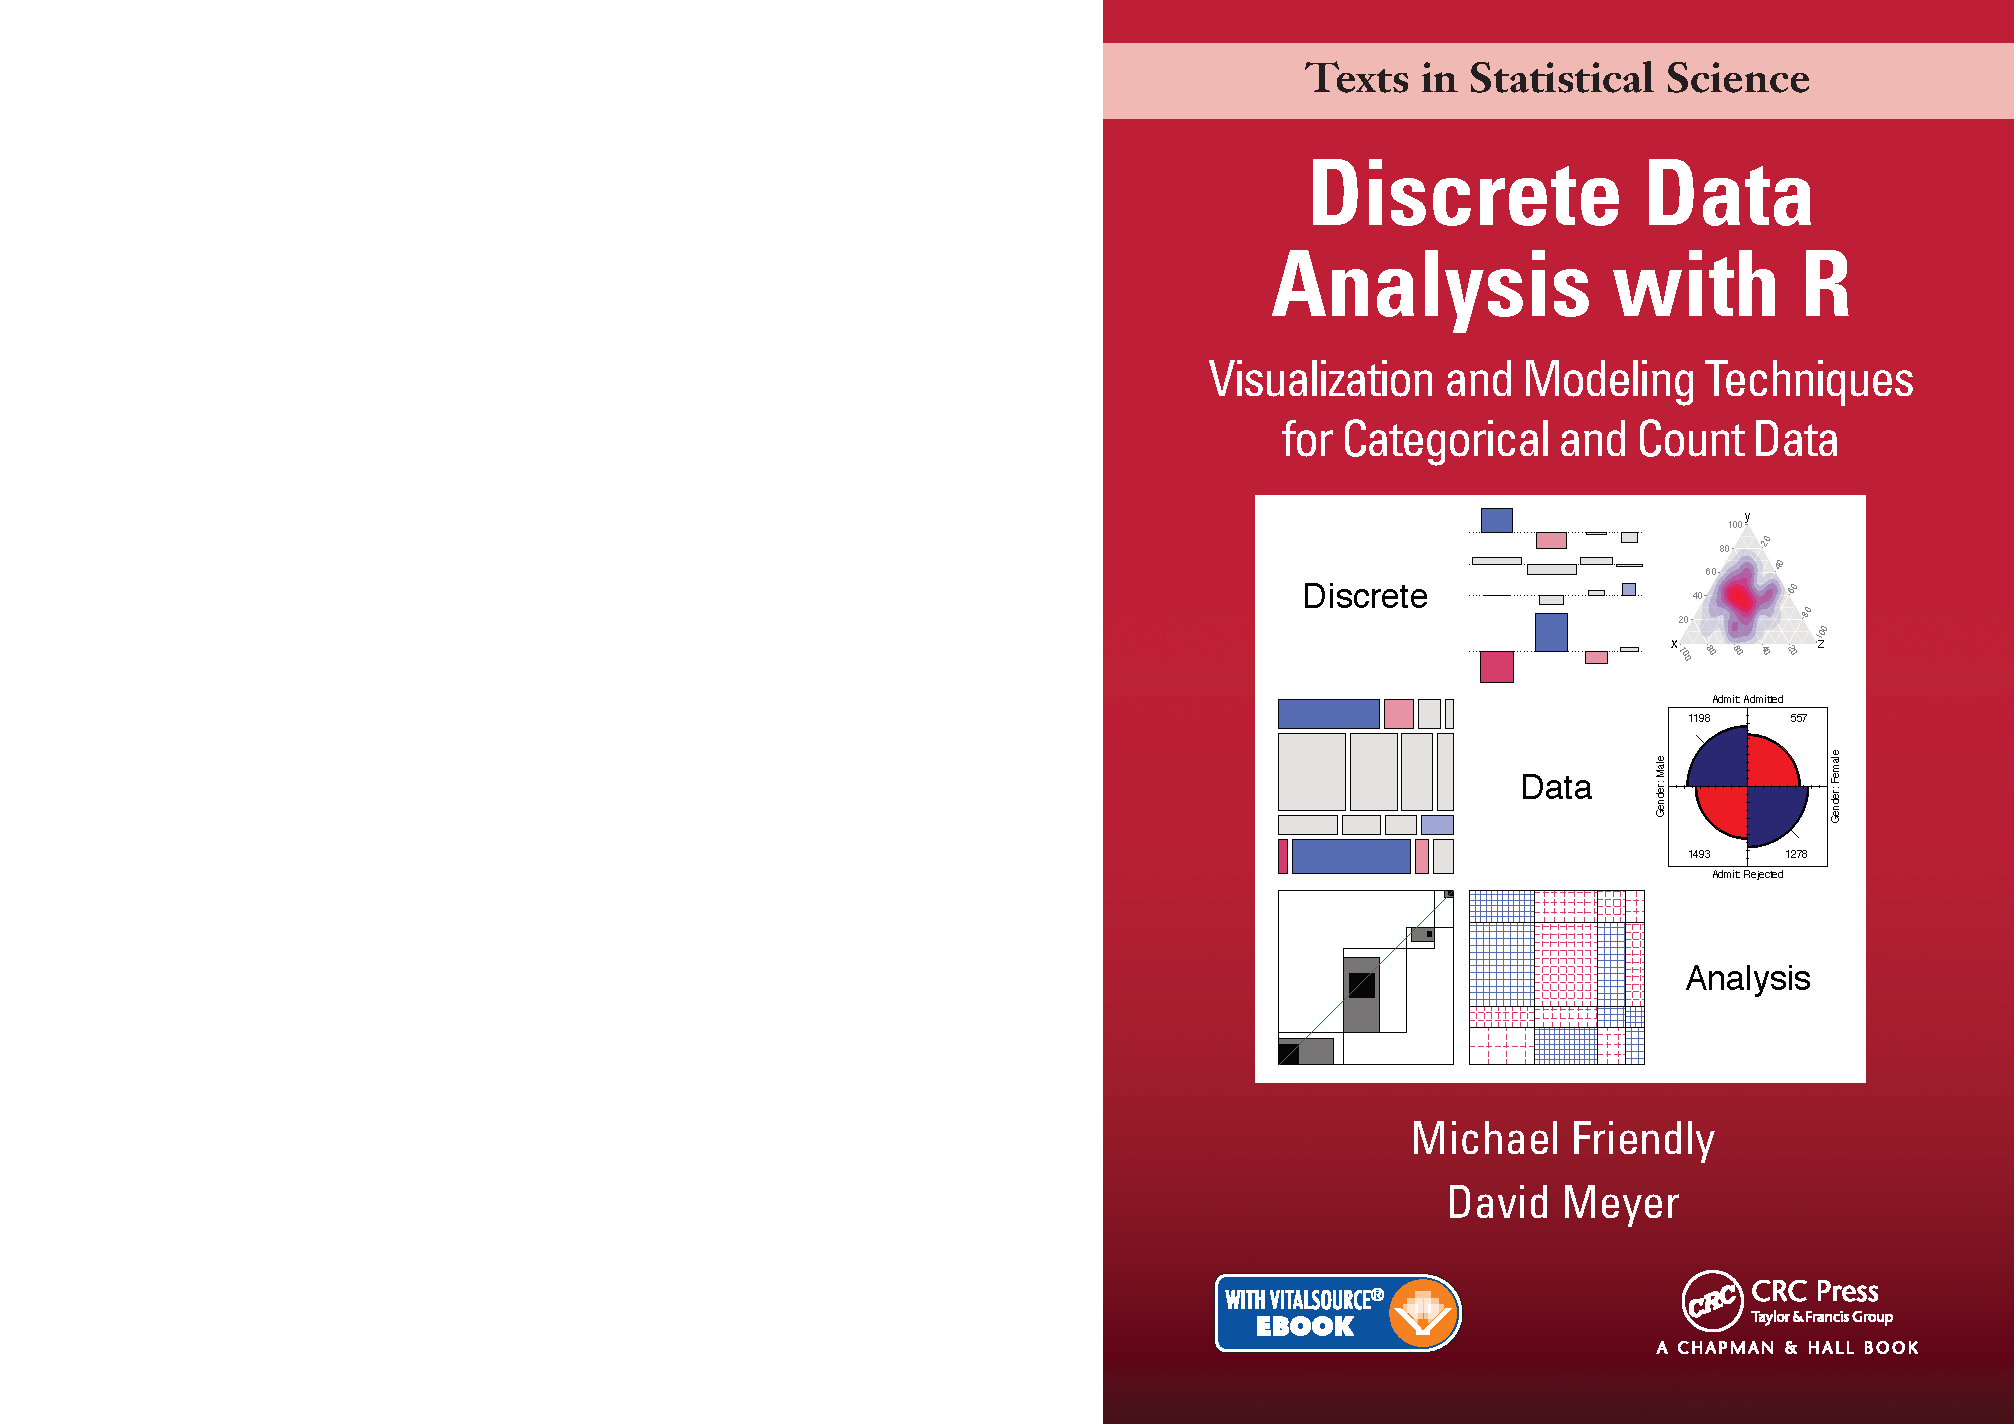
\includegraphics[width=.5\textwidth]{ChapmanHall/K25797_cover-only} 
}

\setcounter{tocdepth}{1}
\IfFileExists{upquote.sty}{\usepackage{upquote}}{}
\begin{document}

\maketitle




\chapter*{\emph{Discrete Data Analysis with R}: \\ Solutions and Hints to Exercises}

{
\renewcommand{\baselinestretch}{.5}\normalsize
\sffamily\small
\tableofcontents
}

\vspace{3em}

\section*{This document}
This document is intended as an aid to instructors who wish to use
\emph{Discrete Data Analysis with R} in a course.  It contains the text
of the \textbf{Exercises} sections from all chapters, together with 
some solutions or hints for the various problems.  Answers and commentary are indicated
with the $\bigstar$ symbol, and \textsf{with text in this font}.

All \R code for the book, and other materials are available on the web site,
\url{http://ddar.datavis.ca}.

\clearpage
\chapter{Introduction}\label{ch:intro}
\begin{ans}
These questions are all conceptual, or based on judgment.  No individual solutions are provided.
In general, students should come up with some interesting examples related to the questions
and explain why they consider them to be good or bad graphic or tabular displays.

Some other sources that students might consult are:
\begin{itemize*}
  \item The Gallery of Data Visualization, \url{http://datavis.ca/gallery/}. A categorized
  collection of some of the best and worst of statistical graphics.
  \item Junk Charts, \url{http://junkcharts.typepad.com/}, a blog by Kaiser Fung.  There
  is also a list of related blogs on graphics and data visualization at
  \url{http://junkcharts.typepad.com/junk_charts/other-graphics-blogs.html}.
  \item Flowing Data, \url{http://flowingdata.com/}, by Nathan Yau. An eclectic
  collection of examples and blog posts encomposing a wide range from information visualization
  to statistical graphics.
\end{itemize*}
\end{ans}

%\section{Lab exercises}\label{sec:ch01-exercises}

\begin{Exercises}

 \exercise A web page, ``The top ten worst graphs, '' \url{http://www.biostat.wisc.edu/~kbroman/topten_worstgraphs/} by Karl Broman lists his picks for the worst graphs (and a table) that have appeared in the
 statistical and scientific literature.  Each entry links to graph(s) and a brief discussion of
 what is wrong and how it could be improved. 
 \begin{enumerate*}
   \item Examine a number of recent issues of a scientific or statistical journal in which you
   have some interest.  Find one or more examples of a graph or table that is a particularly
   bad use of display material to summarize and communicate research findings. Write a
   few sentences indicating how or why the display fails and how it could be improved.
   \item Do the same task for some popular magazine or newspaper that uses data displays
   to supplement the text for some story. Again, write a few sentences describing why the
   display is bad and how it could be improved.
 \end{enumerate*}
 
 \exercise As in the previous exercise, examine the recent literature in recent issues of some
 journal of interest to you.  Find one or more examples of a graph or table that you feel
 does a \emph{good} of summarizing and communicating research findings.
 \begin{enumerate*}
   \item Write a few sentences describing why you chose these displays.
   \item Now take the role of a tough journal reviewer.  Are there any features of the
   display that could be modified to make them more effective?
 \end{enumerate*}
 
 \exercise Infographics are another form of visual displays, quite different from the
 data graphics featured in this book, but often based on some data or analysis.
 Do a Google image search for the topic ``Global warming'' to see a rich
 collection.
 \begin{enumerate*}
   \item Find and study one or two that attempt some visual explanation of causes
   and/or effects of global warming.  Describe the main message in a sentence or
   two.
   \item What visual and graphic features are used in these to convey the message?
 \end{enumerate*}

 \exercise The Wikipedia web page \url{en.wikipedia.org/wiki/Portal:Global_warming}
   gives a few data-based graphics on the topic of global warming.  
   Read the text and study the graphs.  
   \begin{enumerate*}
	   \item Write a short figure title for each that would announce the conclusion
	   to be drawn in a presentation graphic.  
	   \item Write a figure caption for each that 
	   would explain what is shown and the important graphical details for a reader to
	   understand.
   \end{enumerate*}

\end{Exercises}


%' <<exercises01, child="ch01/exercises.Rnw", purl=FALSE>>=
%' @

\chapter{Working with Categorical Data}\label{ch:working}

\begin{Exercises}

\exercise The packages \pkg{vcd} and \pkg{vcdExtra} contain many data sets with some
examples of analysis and graphical display.  The goal of this exercise is to
familiarize yourself with these resources.

You can get a brief summary of
these using the function \func{datasets} from \pkg{vcdExtra}.  Use the following to get a list of
these with some characteristics and titles.
\begin{knitrout}\footnotesize
\definecolor{shadecolor}{rgb}{0.941, 0.941, 0.941}\color{fgcolor}\begin{kframe}
\begin{alltt}
\hlstd{> }\hlstd{ds} \hlkwb{<-} \hlkwd{datasets}\hlstd{(}\hlkwc{package} \hlstd{=} \hlkwd{c}\hlstd{(}\hlstr{"vcd"}\hlstd{,} \hlstr{"vcdExtra"}\hlstd{))}
\hlstd{> }\hlkwd{str}\hlstd{(ds,} \hlkwc{vec.len} \hlstd{=} \hlnum{2}\hlstd{)}
\end{alltt}
\begin{verbatim}
'data.frame':	75 obs. of  5 variables:
 $ Package: chr  "vcd" "vcd" ...
 $ Item   : chr  "Arthritis" "Baseball" ...
 $ class  : chr  "data.frame" "data.frame" ...
 $ dim    : chr  "84x5" "322x25" ...
 $ Title  : chr  "Arthritis Treatment Data" "Baseball Data" ...
\end{verbatim}
\end{kframe}
\end{knitrout}
  \begin{enumerate*}
    \item How many data sets are there altogether?  How many are there in each package?
    \begin{ans}
    \func{nrow} gives the number of rows in a data frame. \func{table} for a single variable gives the frequencies for each level.
\begin{knitrout}\footnotesize
\definecolor{shadecolor}{rgb}{0.941, 0.941, 0.941}\color{fgcolor}\begin{kframe}
\begin{alltt}
\hlstd{> }\hlstd{ds} \hlkwb{<-} \hlkwd{datasets}\hlstd{(}\hlkwc{package}\hlstd{=}\hlkwd{c}\hlstd{(}\hlstr{"vcd"}\hlstd{,} \hlstr{"vcdExtra"}\hlstd{))}
\hlstd{> }\hlkwd{nrow}\hlstd{(ds)}
\end{alltt}
\begin{verbatim}
[1] 75
\end{verbatim}
\begin{alltt}
\hlstd{> }\hlkwd{table}\hlstd{(ds}\hlopt{$}\hlstd{Package)}
\end{alltt}
\begin{verbatim}

     vcd vcdExtra 
      33       42 
\end{verbatim}
\end{kframe}
\end{knitrout}
    \end{ans}
    
    
    \item Make a tabular display of the frequencies by \code{Package} and \code{class}.
    \begin{ans}
    Use \func{table}, but now for \code{Package} and \code{class}.
\begin{knitrout}\footnotesize
\definecolor{shadecolor}{rgb}{0.941, 0.941, 0.941}\color{fgcolor}\begin{kframe}
\begin{alltt}
\hlstd{> }\hlkwd{table}\hlstd{(ds}\hlopt{$}\hlstd{Package, ds}\hlopt{$}\hlstd{class)}
\end{alltt}
\begin{verbatim}
          
           array data.frame matrix table
  vcd          1         17      0    15
  vcdExtra     3         23      1    15
\end{verbatim}
\end{kframe}
\end{knitrout}
    \end{ans}
    
    
    \item Choose one or two data sets from this list, and examine their help files
    (e.g., \code{help(Arthritis)} or \code{?Arthritis}).  You can use, e.g.,
    \code{example(Arthritis)} to run the \R code for a given example.
    \begin{ans}
    Run the following types of commands:
\begin{knitrout}\footnotesize
\definecolor{shadecolor}{rgb}{0.941, 0.941, 0.941}\color{fgcolor}\begin{kframe}
\begin{alltt}
\hlstd{> }\hlopt{?}\hlstd{Arthritis}          \hlcom{# Help Files}
\hlstd{> }\hlopt{?}\hlstd{Baseball}           \hlcom{# Help Files}
\hlstd{> }\hlkwd{example}\hlstd{(Arthritis)}  \hlcom{# Example Syntax/Analysis}
\hlstd{> }\hlkwd{example}\hlstd{(Baseball)}   \hlcom{# Example Syntax/Analysis}
\end{alltt}
\end{kframe}
\end{knitrout}
    \end{ans}
    
    
  \end{enumerate*}

\exercise For each of the following data sets in the \Rpackage{vcdExtra}, identify which are response variable(s)
and which are explanatory. For factor variables, which are unordered (nominal) and which
should be treated as ordered? Write a sentence or two describing substantitive questions of interest for analysis
of the data. (\emph{Hint}: use 
\code{data(foo, package="vcdExtra")} to load, and \code{str(foo)}, 
  \code{help(foo)} to examine data set \code{foo}.)
  \begin{enumerate*}
    \item Abortion opinion data: \data{Abortion}
    \begin{ans}
      \texttt{Support\_Abortion} is the response, \texttt{Sex} and \texttt{Status} are binary, nominal explanatory variables. 
      From \texttt{help(Abortion)},
      How does support for abortion depend on sex and status?
\begin{knitrout}\footnotesize
\definecolor{shadecolor}{rgb}{0.941, 0.941, 0.941}\color{fgcolor}\begin{kframe}
\begin{alltt}
\hlstd{> }\hlkwd{data}\hlstd{(Abortion,} \hlkwc{package}\hlstd{=}\hlstr{"vcdExtra"}\hlstd{)}
\hlstd{> }\hlkwd{str}\hlstd{(Abortion)}
\end{alltt}
\begin{verbatim}
 table [1:2, 1:2, 1:2] 171 152 138 167 79 148 112 133
 - attr(*, "dimnames")=List of 3
  ..$ Sex             : chr [1:2] "Female" "Male"
  ..$ Status          : chr [1:2] "Lo" "Hi"
  ..$ Support_Abortion: chr [1:2] "Yes" "No"
\end{verbatim}
\end{kframe}
\end{knitrout}
    \end{ans}
        
    \item Caesarian Births: \data{Caesar}
    \begin{ans}
      \texttt{Infection} is the response, \texttt{Risk}, \texttt{Antibiotics} and \texttt{Planned} are binary, nominal explanatory
      variables. 
\begin{knitrout}\footnotesize
\definecolor{shadecolor}{rgb}{0.941, 0.941, 0.941}\color{fgcolor}\begin{kframe}
\begin{alltt}
\hlstd{> }\hlkwd{data}\hlstd{(Caesar,} \hlkwc{package}\hlstd{=}\hlstr{"vcdExtra"}\hlstd{)}
\hlstd{> }\hlkwd{str}\hlstd{(Caesar)}
\end{alltt}
\begin{verbatim}
 table [1:3, 1:2, 1:2, 1:2] 0 1 17 0 1 1 11 17 30 4 ...
 - attr(*, "dimnames")=List of 4
  ..$ Infection  : chr [1:3] "Type 1" "Type 2" "None"
  ..$ Risk       : chr [1:2] "Yes" "No"
  ..$ Antibiotics: chr [1:2] "Yes" "No"
  ..$ Planned    : chr [1:2] "Yes" "No"
\end{verbatim}
\end{kframe}
\end{knitrout}
    \end{ans}
        
    \item Dayton Survey: \data{DaytonSurvey}
    \begin{ans}
      In \texttt{DaytonSurvey}, the variables \texttt{cigarette}, \texttt{alcohol}, and \texttt{marijuana} can all be treated as
      response variables.
      \texttt{sex} and \texttt{race} are potential explanatory variables. Potentially interesting questions are how
      each of the responses depend on \texttt{sex} and \texttt{race}, and how they vary jointly.
\begin{knitrout}\footnotesize
\definecolor{shadecolor}{rgb}{0.941, 0.941, 0.941}\color{fgcolor}\begin{kframe}
\begin{alltt}
\hlstd{> }\hlkwd{data}\hlstd{(DaytonSurvey,} \hlkwc{package}\hlstd{=}\hlstr{"vcdExtra"}\hlstd{)}
\hlstd{> }\hlkwd{str}\hlstd{(DaytonSurvey)}
\end{alltt}
\end{kframe}
\end{knitrout}
    \end{ans}
        
    \item Minnesota High School Graduates: \data{Hoyt}
    \begin{ans}
      \texttt{Status} is the response, \texttt{Rank}, \texttt{Occupation}, and \texttt{Sex} are explanatory variables. 
      Both \texttt{Rank} and \texttt{Occupation} are ordinal. How does \texttt{Status} vary with \texttt{Rank}, \texttt{Occupation}, and \texttt{Sex}?
\begin{knitrout}\footnotesize
\definecolor{shadecolor}{rgb}{0.941, 0.941, 0.941}\color{fgcolor}\begin{kframe}
\begin{alltt}
\hlstd{> }\hlkwd{data}\hlstd{(Hoyt,} \hlkwc{package}\hlstd{=}\hlstr{"vcdExtra"}\hlstd{)}
\hlstd{> }\hlkwd{str}\hlstd{(Hoyt)}
\end{alltt}
\end{kframe}
\end{knitrout}
    \end{ans}    
    
  \end{enumerate*}

\exercise The data set \data{UCBAdmissions} is a 3-way table of frequencies
classified by \var{Admit}, \var{Gender}, and \var{Dept}.
  \begin{enumerate*}
    \item Find the total number of cases contained in this table.
    \begin{ans}
      For a \texttt{table} object, just use \texttt{sum()}
\begin{knitrout}\footnotesize
\definecolor{shadecolor}{rgb}{0.941, 0.941, 0.941}\color{fgcolor}\begin{kframe}
\begin{alltt}
\hlstd{> }\hlkwd{data}\hlstd{(UCBAdmissions)}
\hlstd{> }\hlkwd{sum}\hlstd{(UCBAdmissions)}
\end{alltt}
\begin{verbatim}
[1] 4526
\end{verbatim}
\end{kframe}
\end{knitrout}
    \end{ans}
        
    \item For each department, find the total number of applicants.
    \begin{ans}
      Use \code{margin.table(UCBAdmissions, 3)} to find the marginal total for the third dimension (\code{dept}).
\begin{knitrout}\footnotesize
\definecolor{shadecolor}{rgb}{0.941, 0.941, 0.941}\color{fgcolor}\begin{kframe}
\begin{alltt}
\hlstd{> }\hlkwd{margin.table}\hlstd{(UCBAdmissions,} \hlnum{3}\hlstd{)}
\end{alltt}
\begin{verbatim}
Dept
  A   B   C   D   E   F 
933 585 918 792 584 714 
\end{verbatim}
\end{kframe}
\end{knitrout}

    \end{ans}
        
    \item For each department, find the overall proportion of applicants who were admitted.
    \begin{ans}
\begin{knitrout}\footnotesize
\definecolor{shadecolor}{rgb}{0.941, 0.941, 0.941}\color{fgcolor}\begin{kframe}
\begin{alltt}
\hlstd{> }\hlstd{ucb.df} \hlkwb{<-} \hlkwd{as.data.frame}\hlstd{(UCBAdmissions)}
\hlstd{> }\hlstd{abd} \hlkwb{<-} \hlkwd{xtabs}\hlstd{(Freq} \hlopt{~} \hlstd{Dept} \hlopt{+} \hlstd{Admit,} \hlkwc{data}\hlstd{=ucb.df)}
\hlstd{> }\hlkwd{prop.table}\hlstd{(abd,} \hlnum{1}\hlstd{)}
\end{alltt}
\begin{verbatim}
    Admit
Dept Admitted Rejected
   A 0.644159 0.355841
   B 0.632479 0.367521
   C 0.350763 0.649237
   D 0.339646 0.660354
   E 0.251712 0.748288
   F 0.064426 0.935574
\end{verbatim}
\end{kframe}
\end{knitrout}
    \end{ans}
        
    \item Construct a tabular display of department (rows) and gender (columns), showing
    the proportion of applicants in each cell who were admitted
    relative to the total applicants in that cell.
    \begin{ans}
    \end{ans}
        
  \end{enumerate*}
% \begin{answer}
% 	\begin{enumerate*}
% 		\item Use \code{sum(UCBAdmissions)}.
% 		\item Use \code{margin.table(UCBAdmissions, 3)} to find the marginal total for the third dimension (\code{dept}).
% 		\item
% 	\end{enumerate*}
% \end{answer}

\exercise The data set \data{DanishWelfare} in \pkg{vcd} 
gives a 4-way, $3 \times 4 \times 3 \times 5$ 
table as a data frame in
frequency form, containing the variable \var{Freq} and four factors,
\var{Alcohol},
\var{Income},
\var{Status}, and
\var{Urban}.  The variable \var{Alcohol} can be considered as the
response variable, and the others as possible predictors.

  \begin{enumerate*}
    \item Find the total number of cases represented in this table.
    \begin{ans}
      This is a data set in the form of a frequency data.frame, so sum the \texttt{Freq} variable
\begin{knitrout}\footnotesize
\definecolor{shadecolor}{rgb}{0.941, 0.941, 0.941}\color{fgcolor}\begin{kframe}
\begin{alltt}
\hlstd{> }\hlkwd{data}\hlstd{(}\hlstr{"DanishWelfare"}\hlstd{,} \hlkwc{package}\hlstd{=}\hlstr{"vcd"}\hlstd{)}
\hlstd{> }\hlkwd{sum}\hlstd{(DanishWelfare}\hlopt{$}\hlstd{Freq)}
\end{alltt}
\begin{verbatim}
[1] 5144
\end{verbatim}
\end{kframe}
\end{knitrout}
    \end{ans}
        
    \item In this form, the variables \var{Alcohol} and \var{Income}
    should arguably be considered \emph{ordered} factors.  Change them
    to make them ordered.
    \begin{ans}
      Use \texttt{ordered()} or \texttt{as.ordered()} on the factor variable.  \texttt{str()} will then show them as 
      \texttt{Ord.factor}.
\begin{knitrout}\footnotesize
\definecolor{shadecolor}{rgb}{0.941, 0.941, 0.941}\color{fgcolor}\begin{kframe}
\begin{alltt}
\hlstd{> }\hlkwd{levels}\hlstd{(DanishWelfare}\hlopt{$}\hlstd{Alcohol)}
\end{alltt}
\begin{verbatim}
[1] "<1"  "1-2" ">2" 
\end{verbatim}
\begin{alltt}
\hlstd{> }\hlstd{DanishWelfare}\hlopt{$}\hlstd{Alcohol} \hlkwb{<-} \hlkwd{as.ordered}\hlstd{(DanishWelfare}\hlopt{$}\hlstd{Alcohol)}
\hlstd{> }\hlstd{DanishWelfare}\hlopt{$}\hlstd{Income} \hlkwb{<-} \hlkwd{as.ordered}\hlstd{(DanishWelfare}\hlopt{$}\hlstd{Income)}
\hlstd{> }\hlkwd{str}\hlstd{(DanishWelfare)}
\end{alltt}
\begin{verbatim}
'data.frame':	180 obs. of  5 variables:
 $ Freq   : num  1 4 1 8 6 14 8 41 100 175 ...
 $ Alcohol: Ord.factor w/ 3 levels "<1"<"1-2"<">2": 1 1 1 1 1 1 1 1 1 1 ...
 $ Income : Ord.factor w/ 4 levels "0-50"<"50-100"<..: 1 1 1 1 1 1 1 1 1 1 ...
 $ Status : Factor w/ 3 levels "Widow","Married",..: 1 1 1 1 1 2 2 2 2 2 ...
 $ Urban  : Factor w/ 5 levels "Copenhagen","SubCopenhagen",..: 1 2 3 4 5 1 2 3 4 5 ...
\end{verbatim}
\end{kframe}
\end{knitrout}
    \end{ans}
        
    \item Convert this data frame to table form, \code{DanishWelfare.tab},
    a 4-way array containing the
    frequencies with appropriate variable names and level names.
    \begin{ans}
      Use \texttt{xtabs()} with \texttt{Freq} as the response.
      
\begin{knitrout}\footnotesize
\definecolor{shadecolor}{rgb}{0.941, 0.941, 0.941}\color{fgcolor}\begin{kframe}
\begin{alltt}
\hlstd{> }\hlstd{DanishWelfare.tab} \hlkwb{<-}\hlkwd{xtabs}\hlstd{(Freq} \hlopt{~} \hlstd{.,} \hlkwc{data} \hlstd{= DanishWelfare)}
\hlstd{> }\hlkwd{str}\hlstd{(DanishWelfare.tab)}
\end{alltt}
\begin{verbatim}
 xtabs [1:3, 1:4, 1:3, 1:5] 1 3 2 8 1 3 2 5 2 42 ...
 - attr(*, "dimnames")=List of 4
  ..$ Alcohol: chr [1:3] "<1" "1-2" ">2"
  ..$ Income : chr [1:4] "0-50" "50-100" "100-150" ">150"
  ..$ Status : chr [1:3] "Widow" "Married" "Unmarried"
  ..$ Urban  : chr [1:5] "Copenhagen" "SubCopenhagen" "LargeCity" "City" ...
 - attr(*, "class")= chr [1:2] "xtabs" "table"
 - attr(*, "call")= language xtabs(formula = Freq ~ ., data = DanishWelfare)
\end{verbatim}
\end{kframe}
\end{knitrout}
    \end{ans}
    
    \item The variable \var{Urban} has 5 categories.  Find the total frequencies
    in each of these.  How would you collapse the table to have only
    two categories, \code{City}, \code{Non-city}?
    \begin{ans}
      \texttt{margin.table()} handles the first part; \texttt{collapse.table()} is designed for the second part. 
      It is arguable whether
      \texttt{SubCopenhagen} should be considered City or NonCity.
\begin{knitrout}\footnotesize
\definecolor{shadecolor}{rgb}{0.941, 0.941, 0.941}\color{fgcolor}\begin{kframe}
\begin{alltt}
\hlstd{> }\hlkwd{margin.table}\hlstd{(DanishWelfare.tab,} \hlnum{4}\hlstd{)}
\end{alltt}
\begin{verbatim}
Urban
   Copenhagen SubCopenhagen     LargeCity          City       Country 
          552           614           594          1765          1619 
\end{verbatim}
\begin{alltt}
\hlstd{> }\hlstd{DW2} \hlkwb{<-} \hlstd{vcdExtra}\hlopt{::}\hlkwd{collapse.table}\hlstd{(DanishWelfare.tab,}
\hlstd{+ }                                \hlkwc{Urban}\hlstd{=}\hlkwd{c}\hlstd{(}\hlstr{"City"}\hlstd{,}\hlstr{"NonCity"}\hlstd{,}\hlstr{"City"}\hlstd{,}\hlstr{"City"}\hlstd{,}\hlstr{"NonCity"}\hlstd{))}
\hlstd{> }\hlkwd{head}\hlstd{(}\hlkwd{ftable}\hlstd{(DW2))}
\end{alltt}
\begin{verbatim}
                                                         
                                 "Urban" "City" "NonCity"
 "Alcohol" "Income"  "Status"                            
 "<1"      "0-50"    "Widow"                 10        10
                     "Married"              155       183
                     "Unmarried"             14        10
           "50-100"  "Widow"                 29         7
                     "Married"              338       306
                     "Unmarried"             36        32
\end{verbatim}
\end{kframe}
\end{knitrout}
    \end{ans}
    
    \item Use \func{structable} or \func{ftable} to produce a pleasing
    flattened display of the frequencies in the 4-way table.  Choose the
    variables used as row and column variables to make it easier to compare
    levels of \var{Alcohol} across the other factors.
    \begin{ans}
    \end{ans}
    
  \end{enumerate*}

\exercise The data set \data{UKSoccer} in \pkg{vcd} gives the distributions of
number of goals scored by the 20 teams in the  1995/96 season of the
Premier League of the UK Football Association.
\begin{knitrout}\footnotesize
\definecolor{shadecolor}{rgb}{0.941, 0.941, 0.941}\color{fgcolor}\begin{kframe}
\begin{alltt}
\hlstd{> }\hlkwd{data}\hlstd{(}\hlstr{"UKSoccer"}\hlstd{,} \hlkwc{package} \hlstd{=} \hlstr{"vcd"}\hlstd{)}
\hlstd{> }\hlkwd{ftable}\hlstd{(UKSoccer)}
\end{alltt}
\begin{verbatim}
     Away  0  1  2  3  4
Home                    
0         27 29 10  8  2
1         59 53 14 12  4
2         28 32 14 12  4
3         19 14  7  4  1
4          7  8 10  2  0
\end{verbatim}
\end{kframe}
\end{knitrout}
This two-way table classifies all $20 \times 19 = 380$ games by the joint
outcome (Home, Away), the number of goals scored by the \code{Home} and
\code{Away} teams.
The value \code{4} in this table actually represents 4 or more goals.

  \begin{enumerate*}
    \item Verify that the total number of games represented in this table is 380.
    \begin{ans}
\begin{knitrout}\footnotesize
\definecolor{shadecolor}{rgb}{0.941, 0.941, 0.941}\color{fgcolor}\begin{kframe}
\begin{alltt}
\hlstd{> }\hlkwd{data}\hlstd{(}\hlstr{"UKSoccer"}\hlstd{,} \hlkwc{package}\hlstd{=}\hlstr{"vcd"}\hlstd{)}
\hlstd{> }\hlkwd{sum}\hlstd{(UKSoccer)}
\end{alltt}
\begin{verbatim}
[1] 380
\end{verbatim}
\begin{alltt}
\hlstd{> }\hlkwd{margin.table}\hlstd{(UKSoccer)}
\end{alltt}
\begin{verbatim}
[1] 380
\end{verbatim}
\end{kframe}
\end{knitrout}
    \end{ans}
    
    \item Find the marginal total of the number of goals scored by each of
    the home and away teams.
    \begin{ans}
      Use \texttt{margin.table()} for each dimension:
\begin{knitrout}\footnotesize
\definecolor{shadecolor}{rgb}{0.941, 0.941, 0.941}\color{fgcolor}\begin{kframe}
\begin{alltt}
\hlstd{> }\hlkwd{margin.table}\hlstd{(UKSoccer,} \hlnum{1}\hlstd{)}
\end{alltt}
\begin{verbatim}
Home
  0   1   2   3   4 
 76 142  90  45  27 
\end{verbatim}
\begin{alltt}
\hlstd{> }\hlkwd{margin.table}\hlstd{(UKSoccer,} \hlnum{2}\hlstd{)}
\end{alltt}
\begin{verbatim}
Away
  0   1   2   3   4 
140 136  55  38  11 
\end{verbatim}
\end{kframe}
\end{knitrout}
    \end{ans}
    
    \item Express each of the marginal totals as proportions.
    \begin{ans}
      Use \texttt{prop.table()} on the result of \texttt{margin.table()} for each dimension:
\begin{knitrout}\footnotesize
\definecolor{shadecolor}{rgb}{0.941, 0.941, 0.941}\color{fgcolor}\begin{kframe}
\begin{alltt}
\hlstd{> }\hlkwd{prop.table}\hlstd{(}\hlkwd{margin.table}\hlstd{(UKSoccer,} \hlnum{1}\hlstd{))}
\end{alltt}
\begin{verbatim}
Home
       0        1        2        3        4 
0.200000 0.373684 0.236842 0.118421 0.071053 
\end{verbatim}
\begin{alltt}
\hlstd{> }\hlkwd{prop.table}\hlstd{(}\hlkwd{margin.table}\hlstd{(UKSoccer,} \hlnum{2}\hlstd{))}
\end{alltt}
\begin{verbatim}
Away
       0        1        2        3        4 
0.368421 0.357895 0.144737 0.100000 0.028947 
\end{verbatim}
\end{kframe}
\end{knitrout}
    \end{ans}
    
    \item Comment on the distribution of the numbers of home-team and away-team
    goals.  Is there any evidence that home teams score more goals on average?
    \begin{ans}
      You could find the mean number of goals, weighted by their marginal frequencies.
      On average, home teams score about 0.4 more goals.
\begin{knitrout}\footnotesize
\definecolor{shadecolor}{rgb}{0.941, 0.941, 0.941}\color{fgcolor}\begin{kframe}
\begin{alltt}
\hlstd{> }\hlkwd{weighted.mean}\hlstd{(}\hlnum{0}\hlopt{:}\hlnum{4}\hlstd{,} \hlkwc{w}\hlstd{=}\hlkwd{margin.table}\hlstd{(UKSoccer,}\hlnum{1}\hlstd{))}
\end{alltt}
\begin{verbatim}
[1] 1.4868
\end{verbatim}
\begin{alltt}
\hlstd{> }\hlkwd{weighted.mean}\hlstd{(}\hlnum{0}\hlopt{:}\hlnum{4}\hlstd{,} \hlkwc{w}\hlstd{=}\hlkwd{margin.table}\hlstd{(UKSoccer,}\hlnum{2}\hlstd{))}
\end{alltt}
\begin{verbatim}
[1] 1.0632
\end{verbatim}
\end{kframe}
\end{knitrout}
      Graphically, you could also compare the marginal frequencies in a mosaic plot, or use \texttt{agreementplot()}.
\begin{knitrout}\footnotesize
\definecolor{shadecolor}{rgb}{0.941, 0.941, 0.941}\color{fgcolor}\begin{kframe}
\begin{alltt}
\hlstd{> }\hlstd{margins} \hlkwb{<-} \hlkwd{rbind}\hlstd{(}\hlkwc{home}\hlstd{=}\hlkwd{margin.table}\hlstd{(UKSoccer,}\hlnum{1}\hlstd{),}
\hlstd{+ }                 \hlkwc{away}\hlstd{=}\hlkwd{margin.table}\hlstd{(UKSoccer,}\hlnum{2}\hlstd{))}
\hlstd{> }\hlkwd{names}\hlstd{(}\hlkwd{dimnames}\hlstd{(margins))} \hlkwb{<-} \hlkwd{c}\hlstd{(}\hlstr{"Team"}\hlstd{,} \hlstr{"Goals"}\hlstd{)}
\hlstd{> }\hlstd{margins}
\end{alltt}
\begin{verbatim}
      Goals
Team     0   1  2  3  4
  home  76 142 90 45 27
  away 140 136 55 38 11
\end{verbatim}
\begin{alltt}
\hlstd{> }\hlkwd{mosaic}\hlstd{(margins,} \hlkwc{shade}\hlstd{=}\hlnum{TRUE}\hlstd{)}
\end{alltt}
\end{kframe}

\centerline{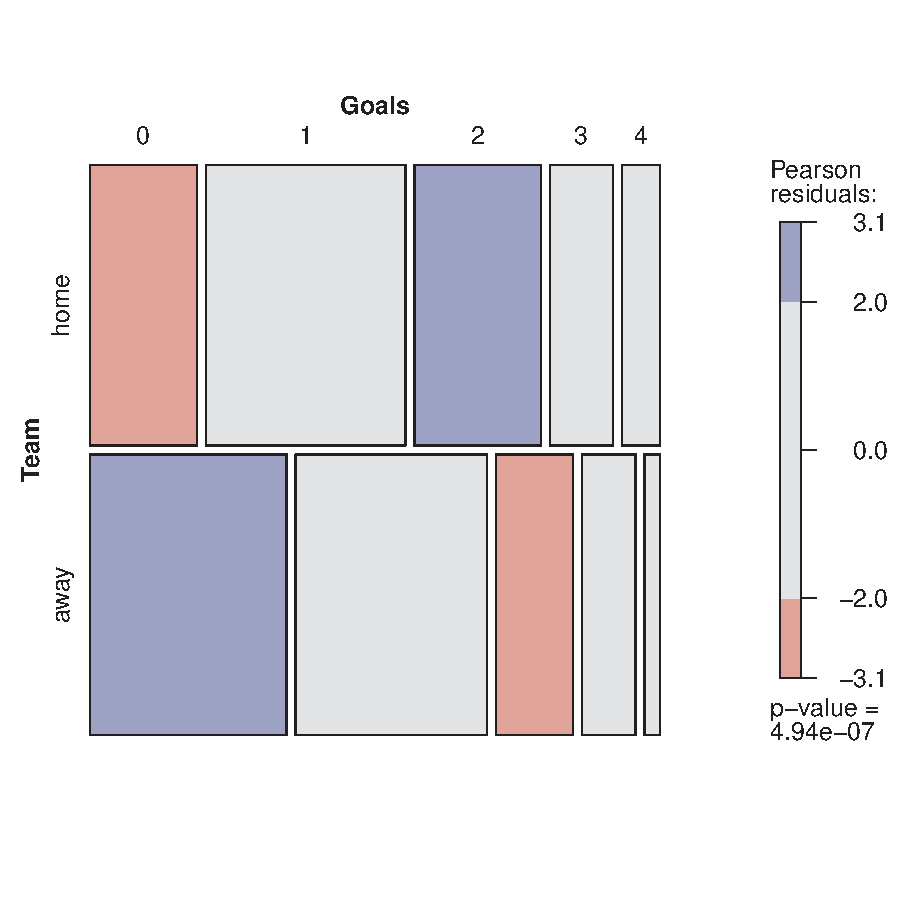
\includegraphics[width=.5\textwidth]{soln/fig/ex2_5d-mosaic-1} }



\end{knitrout}
    \end{ans}
    

  \end{enumerate*}

\exercise The one-way frequency table \data{Saxony} in \pkg{vcd} records the frequencies
of families with 0, 1, 2, $\dots$ 12 male children, among 6115 families with 12
children.  This data set is used extensively in \chref{ch:discrete}.
\begin{knitrout}\footnotesize
\definecolor{shadecolor}{rgb}{0.941, 0.941, 0.941}\color{fgcolor}\begin{kframe}
\begin{alltt}
\hlstd{> }\hlkwd{data}\hlstd{(}\hlstr{"Saxony"}\hlstd{,} \hlkwc{package} \hlstd{=} \hlstr{"vcd"}\hlstd{)}
\hlstd{> }\hlstd{Saxony}
\end{alltt}
\begin{verbatim}
nMales
   0    1    2    3    4    5    6    7    8    9   10   11   12 
   3   24  104  286  670 1033 1343 1112  829  478  181   45    7 
\end{verbatim}
\end{kframe}
\end{knitrout}
Another data set, \data{Geissler}, in the \Rpackage{vcdExtra}, gives the complete
tabulation of all combinations of \code{boys} and \code{girls} in families with
a given total number of children (\code{size}).  The task here is to create an
equivalent table, \code{Saxony12} from the \data{Geissler} data.
\begin{knitrout}\footnotesize
\definecolor{shadecolor}{rgb}{0.941, 0.941, 0.941}\color{fgcolor}\begin{kframe}
\begin{alltt}
\hlstd{> }\hlkwd{data}\hlstd{(}\hlstr{"Geissler"}\hlstd{,} \hlkwc{package} \hlstd{=} \hlstr{"vcdExtra"}\hlstd{)}
\hlstd{> }\hlkwd{str}\hlstd{(Geissler)}
\end{alltt}
\begin{verbatim}
'data.frame':	90 obs. of  4 variables:
 $ boys : int  0 0 0 0 0 0 0 0 0 0 ...
 $ girls: num  1 2 3 4 5 6 7 8 9 10 ...
 $ size : num  1 2 3 4 5 6 7 8 9 10 ...
 $ Freq : int  108719 42860 17395 7004 2839 1096 436 161 66 30 ...
\end{verbatim}
\end{kframe}
\end{knitrout}
  \begin{enumerate*}
    \item Use \func{subset} to create a data frame, \code{sax12} containing
    the \data{Geissler} observations in families with \code{size==12}.
    \begin{ans}
\begin{knitrout}\footnotesize
\definecolor{shadecolor}{rgb}{0.941, 0.941, 0.941}\color{fgcolor}\begin{kframe}
\begin{alltt}
\hlstd{> }\hlkwd{data}\hlstd{(}\hlstr{"Saxony"}\hlstd{,} \hlkwc{package}\hlstd{=}\hlstr{"vcd"}\hlstd{)}
\hlstd{> }\hlkwd{data}\hlstd{(}\hlstr{"Geissler"}\hlstd{,} \hlkwc{package}\hlstd{=}\hlstr{"vcdExtra"}\hlstd{)}
\hlstd{> }\hlstd{sax12} \hlkwb{<-} \hlkwd{subset}\hlstd{(Geissler, size}\hlopt{==}\hlnum{12}\hlstd{)}
\hlstd{> }\hlstd{sax12}
\end{alltt}
\begin{verbatim}
   boys girls size Freq
12    0    12   12    3
24    1    11   12   24
35    2    10   12  104
45    3     9   12  286
54    4     8   12  670
62    5     7   12 1033
69    6     6   12 1343
75    7     5   12 1112
80    8     4   12  829
84    9     3   12  478
87   10     2   12  181
89   11     1   12   45
90   12     0   12    7
\end{verbatim}
\end{kframe}
\end{knitrout}
    \end{ans}
    
    \item Select the columns for \code{boys} and \code{Freq}.
    \begin{ans}
\begin{knitrout}\footnotesize
\definecolor{shadecolor}{rgb}{0.941, 0.941, 0.941}\color{fgcolor}\begin{kframe}
\begin{alltt}
\hlstd{> }\hlstd{sax12} \hlkwb{<-} \hlkwd{subset}\hlstd{(sax12,} \hlkwc{select}\hlstd{=}\hlkwd{c}\hlstd{(}\hlstr{"boys"}\hlstd{,}\hlstr{"Freq"}\hlstd{))}
\end{alltt}
\end{kframe}
\end{knitrout}
    \end{ans}
    
    \item Use \func{xtabs} with a formula, \verb|Freq ~ boys|, to create the
    one-way table.
    \begin{ans}
\begin{knitrout}\footnotesize
\definecolor{shadecolor}{rgb}{0.941, 0.941, 0.941}\color{fgcolor}\begin{kframe}
\begin{alltt}
\hlstd{> }\hlstd{Saxony12}\hlkwb{<-}\hlkwd{xtabs}\hlstd{(Freq}\hlopt{~}\hlstd{boys,} \hlkwc{data}\hlstd{=sax12)}
\hlstd{> }\hlstd{Saxony12}
\end{alltt}
\begin{verbatim}
boys
   0    1    2    3    4    5    6    7    8    9   10   11   12 
   3   24  104  286  670 1033 1343 1112  829  478  181   45    7 
\end{verbatim}
\end{kframe}
\end{knitrout}
    \end{ans}
    
    \item Do the same steps again to create a one-way table, \code{Saxony11},
    containing similar frequencies for families of \code{size==11}.
    \begin{ans}
\begin{knitrout}\footnotesize
\definecolor{shadecolor}{rgb}{0.941, 0.941, 0.941}\color{fgcolor}\begin{kframe}
\begin{alltt}
\hlstd{> }\hlstd{sax11} \hlkwb{<-} \hlkwd{subset}\hlstd{(Geissler, size}\hlopt{==}\hlnum{11}\hlstd{,} \hlkwc{select} \hlstd{=} \hlkwd{c}\hlstd{(}\hlstr{"boys"}\hlstd{,}\hlstr{"Freq"}\hlstd{))}
\hlstd{> }\hlstd{Saxony11} \hlkwb{<-} \hlkwd{xtabs}\hlstd{(Freq}\hlopt{~}\hlstd{boys,} \hlkwc{data}\hlstd{=sax11)}
\hlstd{> }\hlstd{Saxony11}
\end{alltt}
\begin{verbatim}
boys
   0    1    2    3    4    5    6    7    8    9   10   11 
   8   72  275  837 1540 2161 2310 1801 1077  492   93   24 
\end{verbatim}
\end{kframe}
\end{knitrout}
    \end{ans}
    
  \end{enumerate*}

\exercise\exhard \emph{Interactive coding of table factors}:  Some statistical and graphical
methods for \ctabs are implemented only for two-way tables, but can be extended
to 3+-way tables by recoding the factors to interactive combinations along the
rows and/or columns, in a way similar to what \func{ftable} and \func{structable}
do for printed displays.

For the \data{UCBAdmissions} data, produce a two-way table object, \code{UCB.tab2},
that has the combinations of \var{Admit} and \var{Gender} as the rows, and
\var{Dept} as its columns, to look like the result below:
\begin{verbatim}
                 Dept
Admit:Gender        A   B   C   D   E   F
  Admitted:Female  89  17 202 131  94  24
  Admitted:Male   512 353 120 138  53  22
  Rejected:Female  19   8 391 244 299 317
  Rejected:Male   313 207 205 279 138 351
\end{verbatim}
%\emph{Hint}: convert to a data frame, manipulate the factors, then convert back to a table.
  \begin{enumerate*}
    % \begin{sloppypar}
    \item Try this the long way:  convert \data{UCBAdmissions} to a data frame (\func{as.data.frame}),
    manipulate the factors (e.g., \func{interaction}), then convert back to
a table (\func{as.data.frame}).
    % \end{sloppypar}
    \begin{ans}
\begin{knitrout}\footnotesize
\definecolor{shadecolor}{rgb}{0.941, 0.941, 0.941}\color{fgcolor}\begin{kframe}
\begin{alltt}
\hlstd{> }\hlstd{ucb.df}\hlopt{$}\hlstd{AG} \hlkwb{<-} \hlkwd{with}\hlstd{(ucb.df,} \hlkwd{interaction}\hlstd{(Admit, Gender,} \hlkwc{sep}\hlstd{=}\hlstr{":"}\hlstd{))}
\hlstd{> }\hlstd{ucb} \hlkwb{<-} \hlkwd{subset}\hlstd{(ucb.df,} \hlkwc{select} \hlstd{=} \hlkwd{c}\hlstd{(}\hlstr{"Dept"}\hlstd{,} \hlstr{"AG"}\hlstd{,} \hlstr{"Freq"}\hlstd{))}
\hlstd{> }\hlstd{ucb.tab2} \hlkwb{<-} \hlkwd{xtabs}\hlstd{(Freq} \hlopt{~} \hlstd{AG} \hlopt{+} \hlstd{Dept,} \hlkwc{data}\hlstd{=ucb)}
\hlstd{> }\hlstd{ucb.tab2}
\end{alltt}
\begin{verbatim}
                 Dept
AG                  A   B   C   D   E   F
  Admitted:Male   512 353 120 138  53  22
  Rejected:Male   313 207 205 279 138 351
  Admitted:Female  89  17 202 131  94  24
  Rejected:Female  19   8 391 244 299 317
\end{verbatim}
\end{kframe}
\end{knitrout}
    \end{ans}
    
    \item Try this the short way:  both \func{ftable} and \func{structable} have \func{as.matrix}
    methods that convert their result to a matrix.
    \begin{ans}
\begin{knitrout}\footnotesize
\definecolor{shadecolor}{rgb}{0.941, 0.941, 0.941}\color{fgcolor}\begin{kframe}
\begin{alltt}
\hlstd{> }\hlstd{ucb.tab2} \hlkwb{<-} \hlkwd{as.matrix}\hlstd{(}\hlkwd{structable}\hlstd{(Dept} \hlopt{~} \hlstd{Admit} \hlopt{+} \hlstd{Gender,} \hlkwc{data} \hlstd{= UCBAdmissions))}
\hlstd{> }\hlstd{ucb.tab2}
\end{alltt}
\begin{verbatim}
                 Dept
Admit_Gender        A   B   C   D   E   F
  Admitted_Male   512 353 120 138  53  22
  Admitted_Female  89  17 202 131  94  24
  Rejected_Male   313 207 205 279 138 351
  Rejected_Female  19   8 391 244 299 317
\end{verbatim}
\end{kframe}
\end{knitrout}
    \end{ans}
    
  \end{enumerate*}

\exercise The data set \data{VisualAcuity} in \pkg{vcd} gives a $4 \times 4 \times 2$
table as a frequency data frame.
\begin{knitrout}\footnotesize
\definecolor{shadecolor}{rgb}{0.941, 0.941, 0.941}\color{fgcolor}\begin{kframe}
\begin{alltt}
\hlstd{> }\hlkwd{data}\hlstd{(}\hlstr{"VisualAcuity"}\hlstd{,} \hlkwc{package} \hlstd{=} \hlstr{"vcd"}\hlstd{)}
\hlstd{> }\hlkwd{str}\hlstd{(VisualAcuity)}
\end{alltt}
\begin{verbatim}
'data.frame':	32 obs. of  4 variables:
 $ Freq  : num  1520 234 117 36 266 ...
 $ right : Factor w/ 4 levels "1","2","3","4": 1 2 3 4 1 2 3 4 1 2 ...
 $ left  : Factor w/ 4 levels "1","2","3","4": 1 1 1 1 2 2 2 2 3 3 ...
 $ gender: Factor w/ 2 levels "male","female": 2 2 2 2 2 2 2 2 2 2 ...
\end{verbatim}
\end{kframe}
\end{knitrout}
  \begin{enumerate*}
    \item From this, use \func{xtabs} to create two $4\times 4$ frequency tables, one for
each gender.
    \begin{ans}
\begin{knitrout}\footnotesize
\definecolor{shadecolor}{rgb}{0.941, 0.941, 0.941}\color{fgcolor}\begin{kframe}
\begin{alltt}
\hlstd{> }\hlkwd{data}\hlstd{(}\hlstr{"VisualAcuity"}\hlstd{,} \hlkwc{package}\hlstd{=}\hlstr{"vcd"}\hlstd{)}
\hlstd{> }\hlstd{va.tabm} \hlkwb{<-} \hlkwd{xtabs}\hlstd{(Freq} \hlopt{~} \hlstd{right}\hlopt{+}\hlstd{left,} \hlkwc{data} \hlstd{= VisualAcuity,} \hlkwc{subset}\hlstd{=gender}\hlopt{==}\hlstr{"male"}\hlstd{)}
\hlstd{> }\hlstd{va.tabm}
\end{alltt}
\begin{verbatim}
     left
right   1   2   3   4
    1 821 112  85  35
    2 116 494 145  27
    3  72 151 583  87
    4  43  34 106 331
\end{verbatim}
\begin{alltt}
\hlstd{> }\hlstd{va.tabf} \hlkwb{<-} \hlkwd{xtabs}\hlstd{(Freq} \hlopt{~} \hlstd{right}\hlopt{+}\hlstd{left,} \hlkwc{data} \hlstd{= VisualAcuity,} \hlkwc{subset}\hlstd{=gender}\hlopt{==}\hlstr{"female"}\hlstd{)}
\hlstd{> }\hlcom{# or, subset after}
\hlstd{> }\hlstd{va.tab} \hlkwb{<-} \hlkwd{xtabs}\hlstd{(Freq} \hlopt{~} \hlstd{.,} \hlkwc{data} \hlstd{= VisualAcuity)}
\hlstd{> }\hlstd{va.tabm} \hlkwb{<-} \hlstd{va.tab[,,}\hlstr{"male"}\hlstd{]}
\hlstd{> }\hlstd{va.tabf} \hlkwb{<-} \hlstd{va.tab[,,}\hlstr{"female"}\hlstd{]}
\end{alltt}
\end{kframe}
\end{knitrout}
    \end{ans}

    \item Use \func{structable} to create a nicely organized tabular display.
    \begin{ans}
\begin{knitrout}\footnotesize
\definecolor{shadecolor}{rgb}{0.941, 0.941, 0.941}\color{fgcolor}\begin{kframe}
\begin{alltt}
\hlstd{> }\hlkwd{structable}\hlstd{(right} \hlopt{~} \hlstd{left} \hlopt{+} \hlstd{gender,} \hlkwc{data} \hlstd{= va.tab)}
\end{alltt}
\begin{verbatim}
            right    1    2    3    4
left gender                          
1    male          821  116   72   43
     female       1520  234  117   36
2    male          112  494  151   34
     female        266 1512  362   82
3    male           85  145  583  106
     female        124  432 1772  179
4    male           35   27   87  331
     female         66   78  205  492
\end{verbatim}
\end{kframe}
\end{knitrout}
    \end{ans}
    
    \item Use \func{xtable} to create a \LaTeX\ or HTML table.
    \begin{ans}
\begin{knitrout}\footnotesize
\definecolor{shadecolor}{rgb}{0.941, 0.941, 0.941}\color{fgcolor}\begin{kframe}
\begin{alltt}
\hlstd{> }\hlkwd{library}\hlstd{(xtable)}
\hlstd{> }\hlstd{va.xtab} \hlkwb{<-} \hlkwd{xtable}\hlstd{(va.tabm)}
\hlstd{> }\hlkwd{print}\hlstd{(va.xtab,} \hlkwc{type}\hlstd{=}\hlstr{"html"}\hlstd{)}
\end{alltt}
\end{kframe}
\end{knitrout}
    \end{ans}
    
  \end{enumerate*}

\end{Exercises}


\clearpage
\chapter{Fitting and Graphing Discrete Distributions}\label{ch:discrete}

\begin{Exercises}
  \exercise The \data{Arbuthnot} data in \pkg{HistData} (\exref{ex:arbuthnot1}) also
   contains the variable
   \code{Ratio}, giving the ratio of male to female births.
	  \begin{enumerate*}
	    \item Make a plot of \code{Ratio} over \code{Year}, similar to \figref{fig:arbuthnot1}.
	    What features stand out?  Which plot do you prefer to display the tendency for
	    more male births?
	    \begin{ans}
\begin{knitrout}\footnotesize
\definecolor{shadecolor}{rgb}{0.941, 0.941, 0.941}\color{fgcolor}\begin{kframe}
\begin{alltt}
\hlstd{> }\hlkwd{library}\hlstd{(HistData)}
\hlstd{> }\hlkwd{data}\hlstd{(Arbuthnot,} \hlkwc{package} \hlstd{=}\hlstr{"HistData"}\hlstd{)}
\hlstd{> }
\hlstd{> }   \hlcom{# plot of Ratio by Year}
\hlstd{> }\hlkwd{par}\hlstd{(}\hlkwc{mar}\hlstd{=}\hlkwd{c}\hlstd{(}\hlnum{5}\hlstd{,}\hlnum{4}\hlstd{,}\hlnum{1}\hlstd{,}\hlnum{1}\hlstd{)}\hlopt{+}\hlnum{.1}\hlstd{)}
\hlstd{> }\hlkwd{with}\hlstd{(Arbuthnot, \{}
\hlstd{+ }  \hlkwd{plot}\hlstd{(Year, Ratio,} \hlkwc{type}\hlstd{=}\hlstr{'b'}\hlstd{,} \hlkwc{ylim}\hlstd{=}\hlkwd{c}\hlstd{(}\hlnum{.95}\hlstd{,} \hlnum{1.2}\hlstd{),}
\hlstd{+ }       \hlkwc{ylab}\hlstd{=}\hlstr{"Birth Ratio (Male/Female)"}\hlstd{)}
\hlstd{+ }  \hlkwd{abline}\hlstd{(}\hlkwc{h}\hlstd{=}\hlnum{1}\hlstd{,} \hlkwc{col}\hlstd{=}\hlstr{"green"}\hlstd{,} \hlkwc{lwd}\hlstd{=}\hlnum{1}\hlstd{)}
\hlstd{+ }  \hlkwd{abline}\hlstd{(}\hlkwc{h}\hlstd{=}\hlkwd{mean}\hlstd{(Ratio),} \hlkwc{col}\hlstd{=}\hlstr{"red"}\hlstd{)}
\hlstd{+ }  \hlkwd{text}\hlstd{(}\hlkwc{x}\hlstd{=}\hlnum{1660}\hlstd{,} \hlkwc{y}\hlstd{=}\hlnum{1}\hlstd{,} \hlstr{"Equal M/F ratio"}\hlstd{,} \hlkwc{pos}\hlstd{=}\hlnum{1}\hlstd{,} \hlkwc{col}\hlstd{=}\hlstr{"green3"}\hlstd{)}
\hlstd{+ }  \hlstd{Arb.smooth} \hlkwb{<-} \hlkwd{loess.smooth}\hlstd{(Year,Ratio)}
\hlstd{+ }  \hlkwd{lines}\hlstd{(Arb.smooth}\hlopt{$}\hlstd{x, Arb.smooth}\hlopt{$}\hlstd{y,} \hlkwc{col}\hlstd{=}\hlstr{"blue"}\hlstd{,} \hlkwc{lwd}\hlstd{=}\hlnum{2}\hlstd{)}
\hlstd{+ }\hlstd{\})}
\end{alltt}
\end{kframe}

\centerline{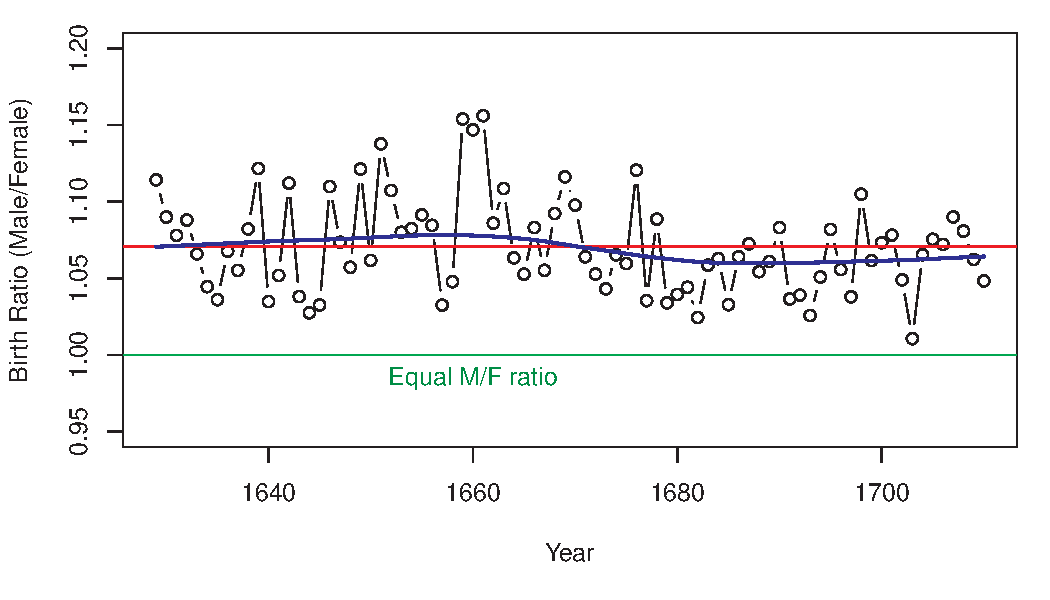
\includegraphics[width=.75\textwidth]{soln/fig/ex3_1a-1} }



\end{knitrout}
			The plot is similar to Figure 3.1 in the text. If it is easier to think in terms of probability of a male birth,
			plotting that directly may be preferable.
	    \end{ans}
	    
	    \item Plot the total number of christenings, \code{Males + Females} or \code{Total}
	    (in 000s) over time.
	    What unusual features do you see?
	    \begin{ans}
\begin{knitrout}\footnotesize
\definecolor{shadecolor}{rgb}{0.941, 0.941, 0.941}\color{fgcolor}\begin{kframe}
\begin{alltt}
\hlstd{> }   \hlcom{# total number of Christenings}
\hlstd{> }\hlkwd{with}\hlstd{(Arbuthnot, \{}
\hlstd{+ }  \hlstd{Total}\hlkwb{=} \hlstd{Males} \hlopt{+} \hlstd{Females}
\hlstd{+ }  \hlkwd{plot}\hlstd{(Year, Total,} \hlkwc{type}\hlstd{=}\hlstr{'b'}\hlstd{,} \hlkwc{ylab}\hlstd{=}\hlstr{"Total Christenings (Male + Female)"}\hlstd{)}
\hlstd{+ }  \hlstd{Arb.smooth} \hlkwb{<-} \hlkwd{loess.smooth}\hlstd{(Year,Total)}
\hlstd{+ }  \hlkwd{lines}\hlstd{(Arb.smooth}\hlopt{$}\hlstd{x, Arb.smooth}\hlopt{$}\hlstd{y,} \hlkwc{col}\hlstd{=}\hlstr{"blue"}\hlstd{,} \hlkwc{lwd}\hlstd{=}\hlnum{2}\hlstd{)}
\hlstd{+ }\hlstd{\})}
\end{alltt}
\end{kframe}

\centerline{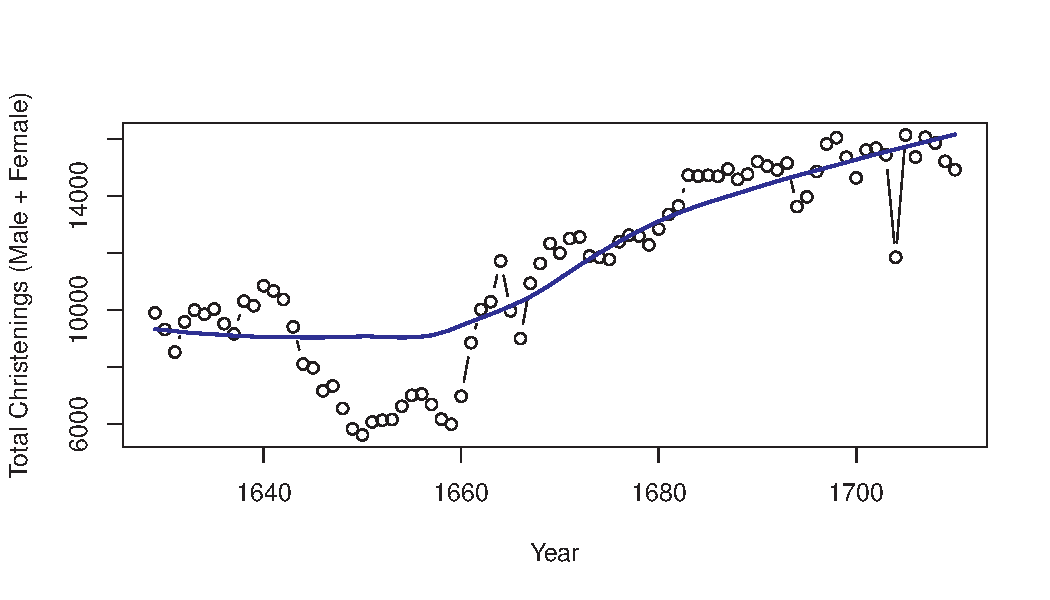
\includegraphics[width=.75\textwidth]{soln/fig/ex3_1b-1} }



\end{knitrout}
			
			There was a large decline in births between 1640--1660, corresponding to years of plague in England.
	    \end{ans}
	    
	  \end{enumerate*}

  \exercise Use the graphical methods illustrated in \secref{sec:discrete-distrib}
  to plot a collection of geometric distributions for $p = 0.2, 0.4, 0.6, 0.8$,
  over a range of values of $k = 0, 1, \dots 10$.
  \begin{enumerate}
    \item With \func{xyplot}, try the different plot formats using points
    connected with lines, as in \figref{fig:dbinom2-plot2}, or using points
    and lines down to the origin, as in the panels of \figref{fig:dpois-xyplot1}.
    \begin{ans}
\begin{knitrout}\footnotesize
\definecolor{shadecolor}{rgb}{0.941, 0.941, 0.941}\color{fgcolor}\begin{kframe}
\begin{alltt}
\hlstd{> }\hlstd{KL} \hlkwb{<-} \hlkwd{expand.grid}\hlstd{(}\hlkwc{k} \hlstd{=} \hlnum{0} \hlopt{:} \hlnum{10}\hlstd{,} \hlkwc{p} \hlstd{=} \hlkwd{c}\hlstd{(}\hlnum{0.2}\hlstd{,} \hlnum{0.4}\hlstd{,} \hlnum{0.6}\hlstd{,} \hlnum{0.8}\hlstd{))}
\hlstd{> }\hlstd{geom_df} \hlkwb{<-} \hlkwd{data.frame}\hlstd{(KL,} \hlkwc{prob} \hlstd{=} \hlkwd{dgeom}\hlstd{(KL}\hlopt{$}\hlstd{k, KL}\hlopt{$}\hlstd{p))}
\hlstd{> }\hlstd{geom_df}\hlopt{$}\hlstd{p} \hlkwb{=} \hlkwd{factor}\hlstd{(geom_df}\hlopt{$}\hlstd{p)}
\hlstd{> }
\hlstd{> }\hlkwd{library}\hlstd{(lattice)}
\hlstd{> }\hlstd{mycol}\hlkwb{<-}\hlkwd{palette}\hlstd{()[}\hlnum{2}\hlopt{:}\hlnum{5}\hlstd{]}
\hlstd{> }\hlkwd{xyplot}\hlstd{(prob} \hlopt{~} \hlstd{k} \hlopt{|} \hlstd{p ,} \hlkwc{data} \hlstd{= geom_df,} \hlkwc{type} \hlstd{=} \hlkwd{c}\hlstd{(}\hlstr{"b"}\hlstd{),}
\hlstd{+ }       \hlkwc{pch} \hlstd{=} \hlnum{16}\hlstd{,} \hlkwc{lwd} \hlstd{=} \hlnum{4}\hlstd{,} \hlkwc{cex} \hlstd{=} \hlnum{1.25}\hlstd{,}
\hlstd{+ }       \hlkwc{xlab} \hlstd{=} \hlkwd{list}\hlstd{(}\hlstr{"Number of events (k)"}\hlstd{,} \hlkwc{cex} \hlstd{=} \hlnum{1.25}\hlstd{),} \hlkwc{layout} \hlstd{=} \hlkwd{c}\hlstd{(}\hlnum{2}\hlstd{,}\hlnum{2}\hlstd{),}
\hlstd{+ }       \hlkwc{ylab} \hlstd{=} \hlkwd{list}\hlstd{(}\hlstr{"Probability"}\hlstd{,} \hlkwc{cex} \hlstd{=} \hlnum{1.25}\hlstd{))}
\hlstd{> }\hlkwd{xyplot}\hlstd{(prob} \hlopt{~} \hlstd{k} \hlopt{|} \hlstd{p ,} \hlkwc{data} \hlstd{= geom_df,} \hlkwc{type} \hlstd{=} \hlkwd{c}\hlstd{(}\hlstr{"h"}\hlstd{,} \hlstr{"p"}\hlstd{),}
\hlstd{+ }       \hlkwc{pch} \hlstd{=} \hlnum{16}\hlstd{,} \hlkwc{lwd} \hlstd{=} \hlnum{4}\hlstd{,} \hlkwc{cex} \hlstd{=} \hlnum{1.25}\hlstd{,}
\hlstd{+ }       \hlkwc{xlab} \hlstd{=} \hlkwd{list}\hlstd{(}\hlstr{"Number of events (k)"}\hlstd{,} \hlkwc{cex} \hlstd{=} \hlnum{1.25}\hlstd{),} \hlkwc{layout} \hlstd{=} \hlkwd{c}\hlstd{(}\hlnum{2}\hlstd{,}\hlnum{2}\hlstd{),}
\hlstd{+ }       \hlkwc{ylab} \hlstd{=} \hlkwd{list}\hlstd{(}\hlstr{"Probability"}\hlstd{,} \hlkwc{cex} \hlstd{=} \hlnum{1.25}\hlstd{))}
\end{alltt}
\end{kframe}

\centerline{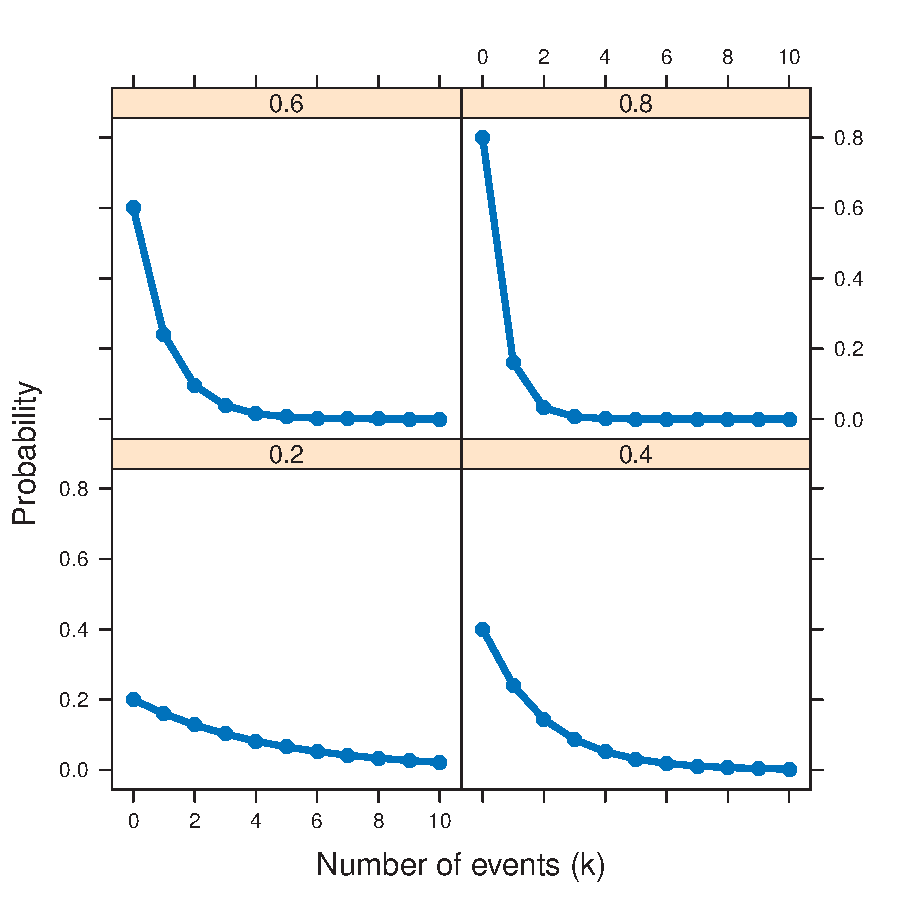
\includegraphics[width=.49\textwidth]{soln/fig/ex3_2a-1} 
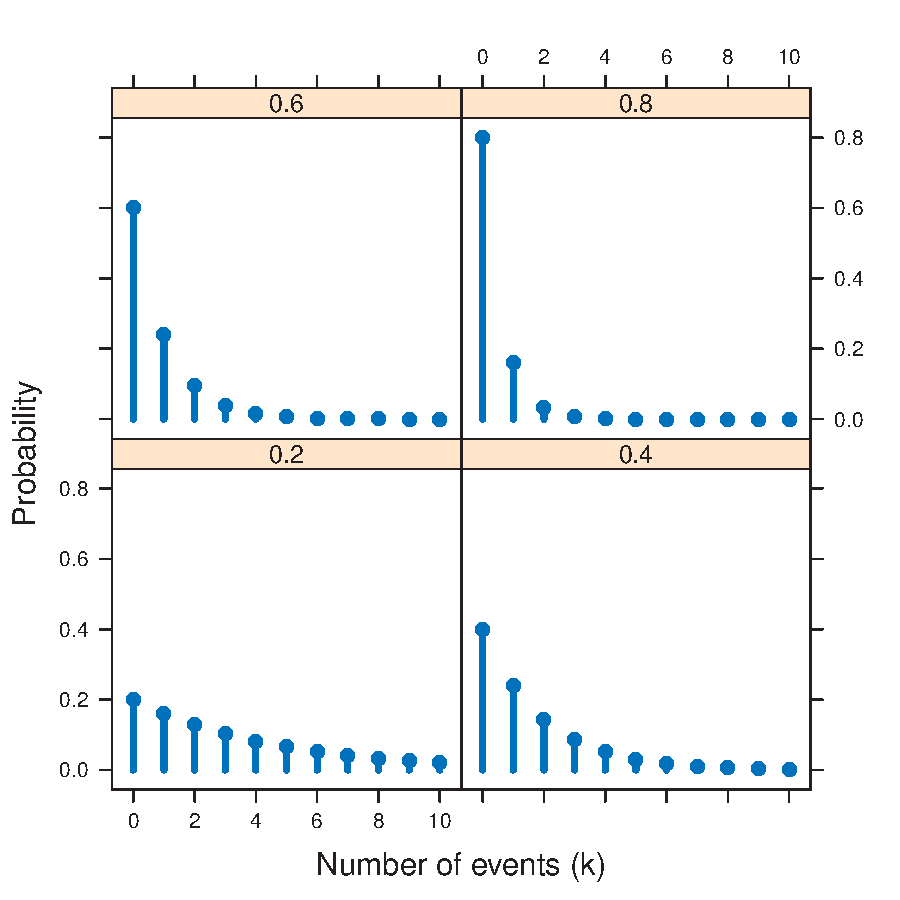
\includegraphics[width=.49\textwidth]{soln/fig/ex3_2a-2} }



\end{knitrout}
    \end{ans}
    
    \item Also with \func{xyplot}, produce one version of a multi-line plot
    in a single panel that you think shows well how these distributions change
    with the probability $p$ of success.
    \begin{ans}
\begin{knitrout}\footnotesize
\definecolor{shadecolor}{rgb}{0.941, 0.941, 0.941}\color{fgcolor}\begin{kframe}
\begin{alltt}
\hlstd{> }\hlstd{geomplt}\hlkwb{<-}\hlkwd{xyplot}\hlstd{(prob} \hlopt{~} \hlstd{k ,} \hlkwc{data} \hlstd{= geom_df,} \hlkwc{groups} \hlstd{= p,}
\hlstd{+ }                \hlkwc{type} \hlstd{=} \hlkwd{c}\hlstd{(}\hlstr{"b"}\hlstd{),} \hlkwc{pch} \hlstd{=} \hlnum{16}\hlstd{,} \hlkwc{lwd} \hlstd{=} \hlnum{4}\hlstd{,} \hlkwc{cex} \hlstd{=} \hlnum{1.25}\hlstd{,} \hlkwc{col} \hlstd{= mycol,}
\hlstd{+ }                \hlkwc{xlab} \hlstd{=} \hlkwd{list}\hlstd{(}\hlstr{"Number of events (k)"}\hlstd{,} \hlkwc{cex} \hlstd{=} \hlnum{1.25}\hlstd{),}
\hlstd{+ }                \hlkwc{ylab} \hlstd{=} \hlkwd{list}\hlstd{(}\hlstr{"Probability"}\hlstd{,} \hlkwc{cex} \hlstd{=} \hlnum{1.25}\hlstd{))}
\hlstd{> }\hlkwd{library}\hlstd{(directlabels)}
\hlstd{> }\hlkwd{direct.label}\hlstd{(geomplt,} \hlkwd{list}\hlstd{(}\hlstr{"top.points"}\hlstd{,} \hlkwc{cex} \hlstd{=} \hlnum{1.25}\hlstd{,} \hlkwd{dl.trans}\hlstd{(}\hlkwc{y} \hlstd{= y} \hlopt{+} \hlnum{0.1}\hlstd{)))}
\end{alltt}
\end{kframe}

\centerline{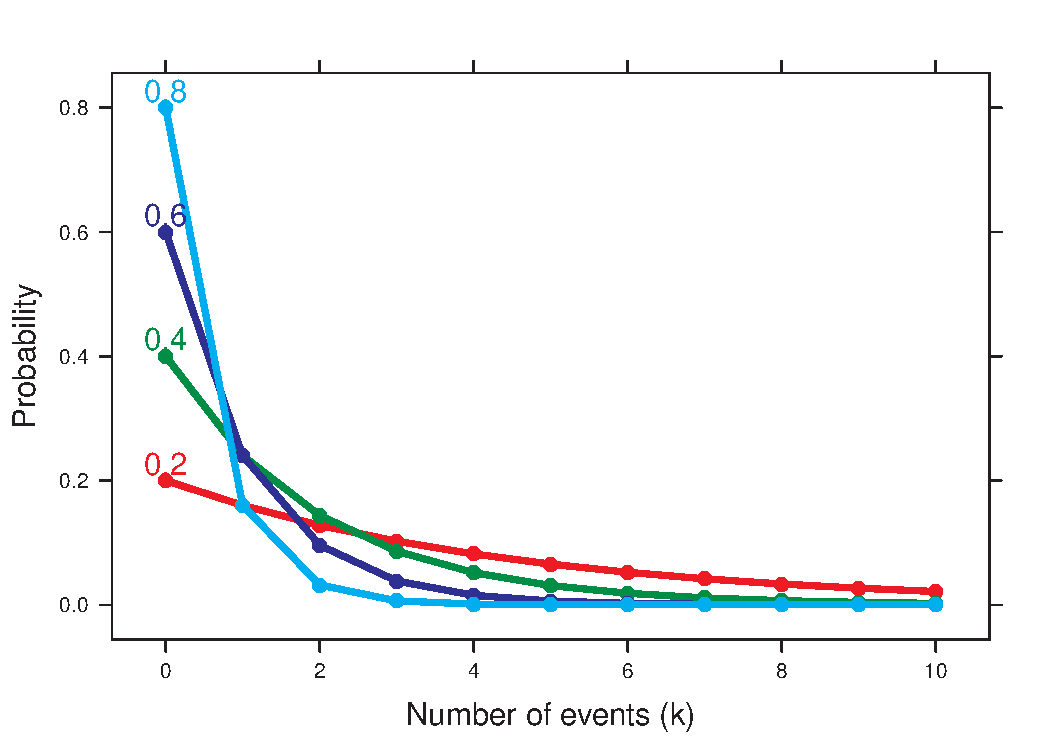
\includegraphics[width=.5\textwidth]{soln/fig/ex3_2b-1} }



\end{knitrout}
    \end{ans}
    
    \item Do the same in a multi-panel version, conditional on $p$.
    \begin{ans}
\begin{knitrout}\footnotesize
\definecolor{shadecolor}{rgb}{0.941, 0.941, 0.941}\color{fgcolor}\begin{kframe}
\begin{alltt}
\hlstd{> }\hlkwd{xyplot}\hlstd{(prob} \hlopt{~} \hlstd{k} \hlopt{|} \hlstd{p ,} \hlkwc{data} \hlstd{= geom_df,} \hlkwc{type} \hlstd{=} \hlkwd{c}\hlstd{(}\hlstr{"b"}\hlstd{),}
\hlstd{+ }       \hlkwc{pch} \hlstd{=} \hlnum{16}\hlstd{,} \hlkwc{lwd} \hlstd{=} \hlnum{4}\hlstd{,} \hlkwc{cex} \hlstd{=} \hlnum{1.25}\hlstd{,}
\hlstd{+ }       \hlkwc{xlab} \hlstd{=} \hlkwd{list}\hlstd{(}\hlstr{"Number of events (k)"}\hlstd{,} \hlkwc{cex} \hlstd{=} \hlnum{1.1}\hlstd{),} \hlkwc{layout} \hlstd{=} \hlkwd{c}\hlstd{(}\hlnum{4}\hlstd{,}\hlnum{1}\hlstd{),}
\hlstd{+ }       \hlkwc{ylab} \hlstd{=} \hlkwd{list}\hlstd{(}\hlstr{"Probability"}\hlstd{,} \hlkwc{cex} \hlstd{=} \hlnum{1.25}\hlstd{))}
\end{alltt}
\end{kframe}

\centerline{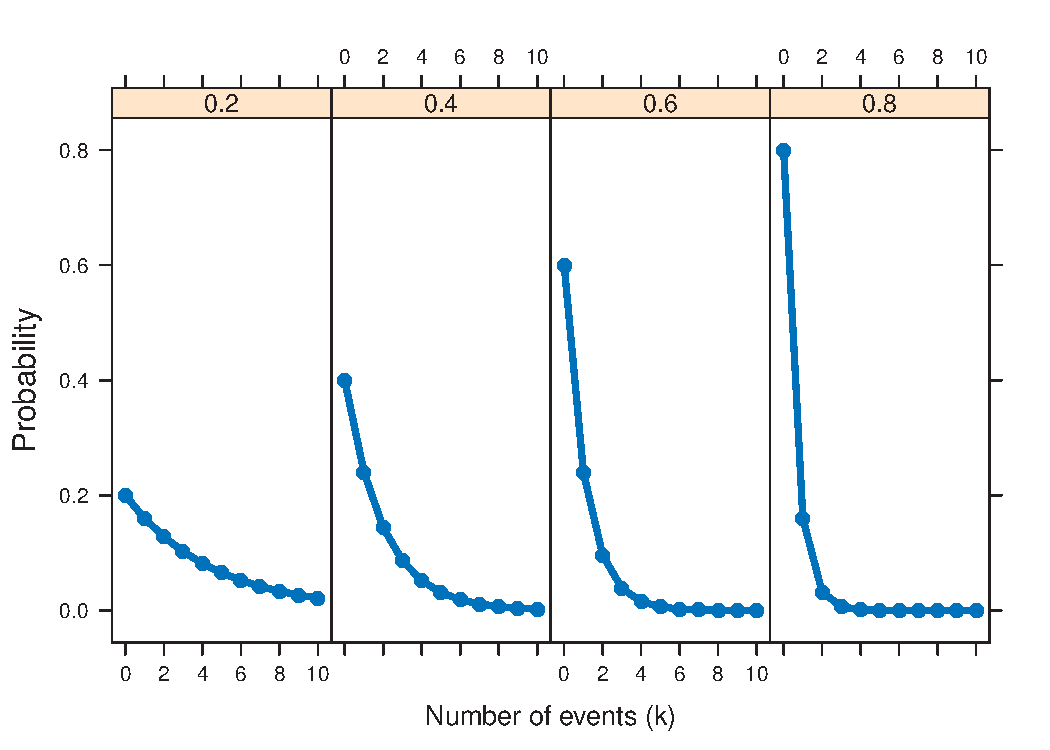
\includegraphics[width=.75\textwidth]{soln/fig/ex3_2c-1} }



\end{knitrout}
    \end{ans}
    
  \end{enumerate}

  \exercise Use the data set \data{WomenQueue} to:
  \begin{enumerate*}
    \item Produce plots analogous to those
  shown in \secref{sec:discrete-intro} (some sort of bar graph of frequencies).
    \begin{ans}
\begin{knitrout}\footnotesize
\definecolor{shadecolor}{rgb}{0.941, 0.941, 0.941}\color{fgcolor}\begin{kframe}
\begin{alltt}
\hlstd{> }\hlkwd{data}\hlstd{(}\hlstr{"WomenQueue"}\hlstd{,} \hlkwc{package} \hlstd{=} \hlstr{"vcd"}\hlstd{)}
\hlstd{> }\hlkwd{barplot}\hlstd{(WomenQueue,} \hlkwc{xlab}\hlstd{=}\hlstr{"Number of Women in queues of 10"}\hlstd{,} \hlkwc{ylab}\hlstd{=} \hlstr{"Frequency"}\hlstd{)}
\end{alltt}
\end{kframe}

\centerline{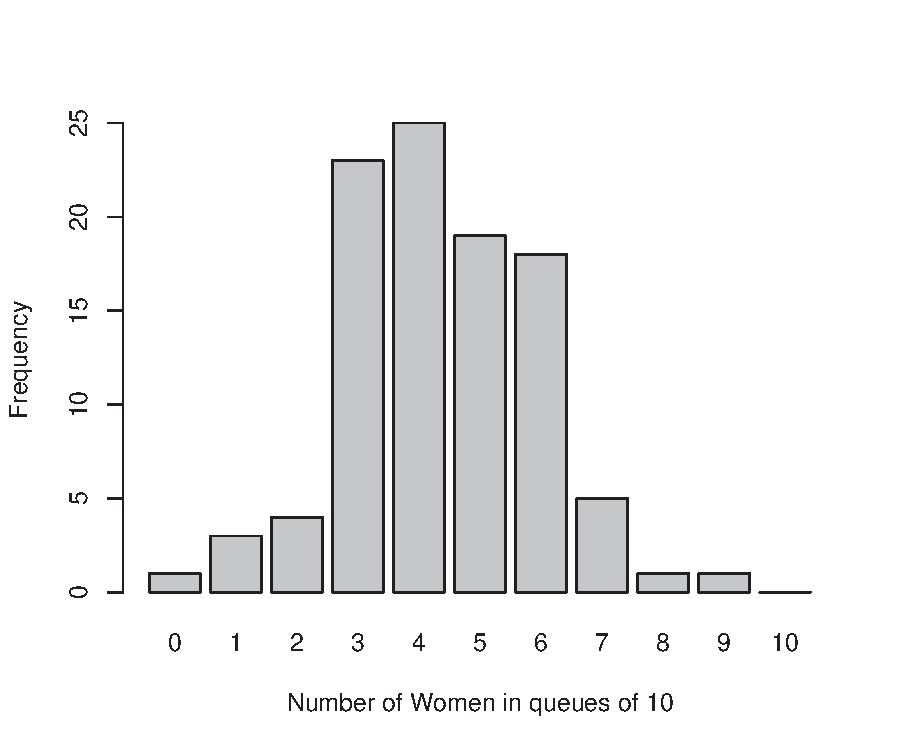
\includegraphics[width=.5\textwidth]{soln/fig/ex3_3a-1} }



\end{knitrout}
    \end{ans}

    \item Check for goodness-of-fit to the binomial distribution using the
    \func{goodfit} methods described in \secref{sec:fitplot}.
    \begin{ans}
    Note that with \texttt{goodfit()}, you should specify $n=10$ for the binomial distribution as the \texttt{size} parameter.
\begin{knitrout}\footnotesize
\definecolor{shadecolor}{rgb}{0.941, 0.941, 0.941}\color{fgcolor}\begin{kframe}
\begin{alltt}
\hlstd{> }\hlkwd{library}\hlstd{(vcd)}
\hlstd{> }\hlstd{gf.women} \hlkwb{<-} \hlkwd{goodfit}\hlstd{(WomenQueue,} \hlkwc{type} \hlstd{=} \hlstr{"binomial"}\hlstd{,} \hlkwc{par}\hlstd{=}\hlkwd{list}\hlstd{(}\hlkwc{size}\hlstd{=}\hlnum{10}\hlstd{))}
\hlstd{> }\hlkwd{summary}\hlstd{(gf.women)}
\end{alltt}
\begin{verbatim}

	 Goodness-of-fit test for binomial distribution

                   X^2 df P(> X^2)
Likelihood Ratio 8.651  8  0.37259
\end{verbatim}
\end{kframe}
\end{knitrout}
    \end{ans}
    
    \item Make a reasonable plot showing departure from the binomial distribution.
    \begin{ans}
The simplest plot is the hanging rootogram.  An alternative plot is a "binomialness" plot produced by \texttt{distplot()}.
\begin{knitrout}\footnotesize
\definecolor{shadecolor}{rgb}{0.941, 0.941, 0.941}\color{fgcolor}\begin{kframe}
\begin{alltt}
\hlstd{> }\hlkwd{plot}\hlstd{(gf.women,} \hlkwc{xlab} \hlstd{=} \hlstr{"Queue Length"}\hlstd{)}
\hlstd{> }\hlkwd{distplot}\hlstd{(WomenQueue,} \hlkwc{type} \hlstd{=} \hlstr{"binomial"}\hlstd{,} \hlkwc{size}\hlstd{=}\hlnum{10}\hlstd{,} \hlkwc{xlab} \hlstd{=} \hlstr{"Queue Length"}\hlstd{)}
\end{alltt}
\end{kframe}

\centerline{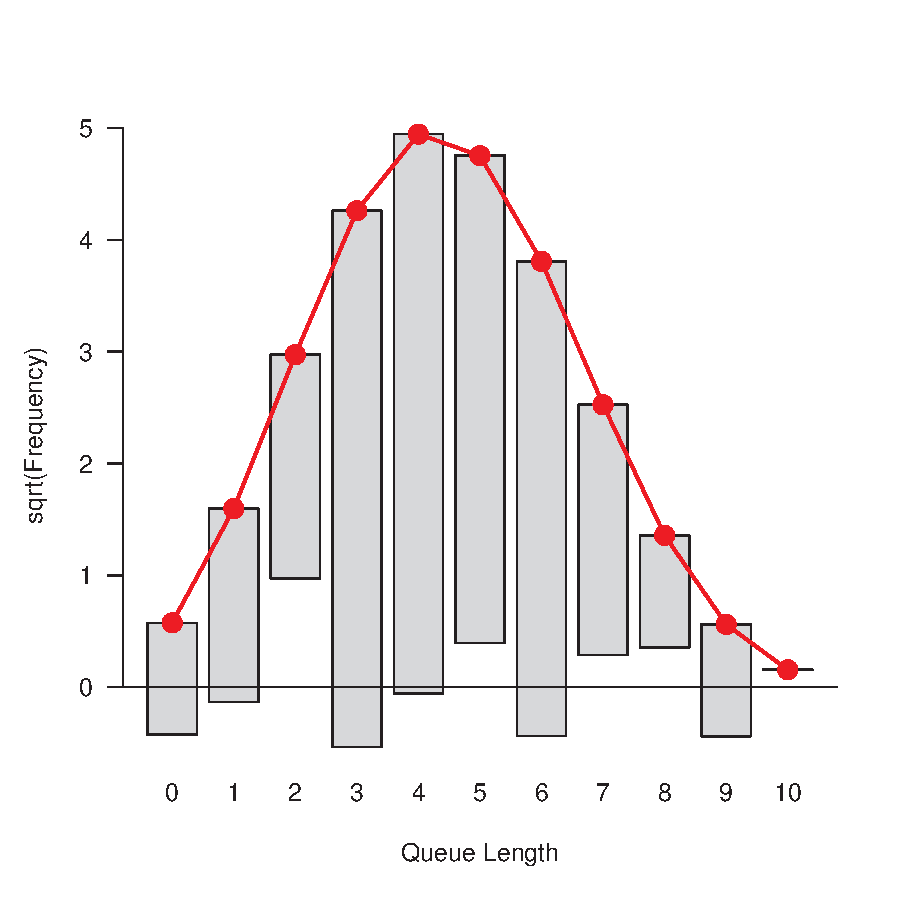
\includegraphics[width=.49\textwidth]{soln/fig/ex3_3c-1} 
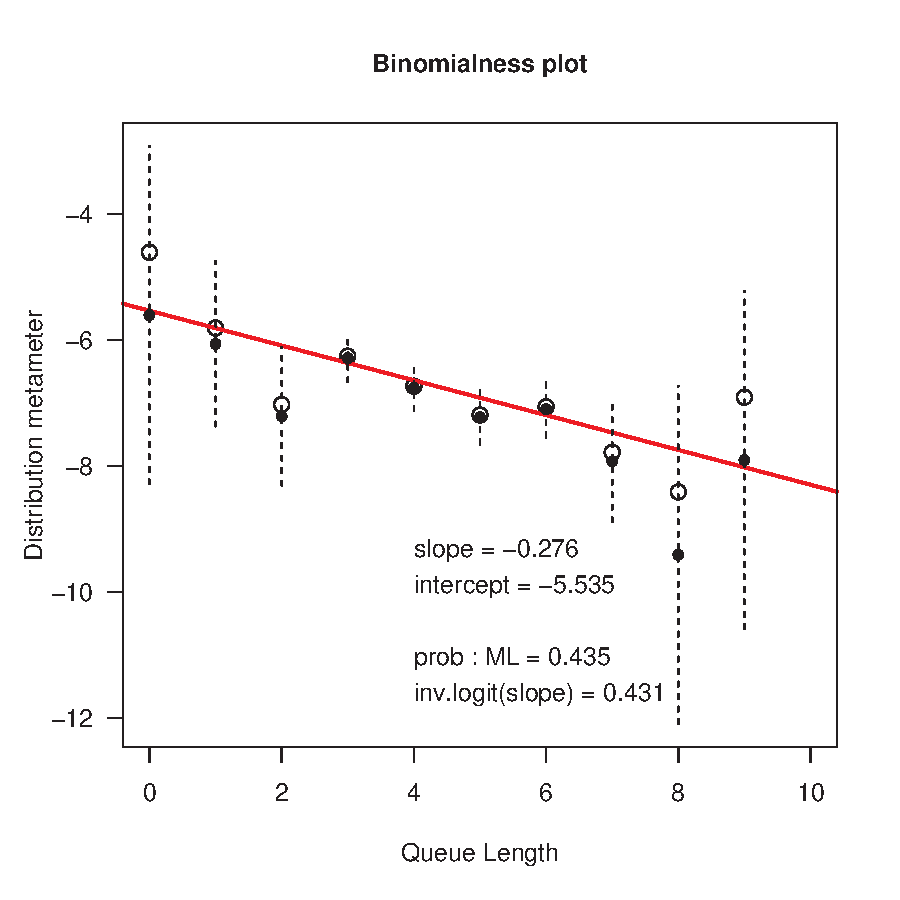
\includegraphics[width=.49\textwidth]{soln/fig/ex3_3c-2} }



\end{knitrout}
    \end{ans}
    
    \item Suggest some reasons why the number of women in queues of length 10
    might depart from a binomial distribution, $\Bin(n=10, p=1/2)$.
    \begin{ans}
    \begin{itemize*}
      \item Perhaps women (or men) are more prevalent in these queues, so $p \ne 1/2$.
      \item People often join lines in groups, so the observations are unlikely to be independent.
    \end{itemize*}
    \end{ans}
    
  \end{enumerate*}

  \exercise Continue \exref{ex:saxfit} on the distribution of male children in families
  in Saxony by fitting a binomial distribution, $\Bin(n=12, p=\frac12)$, specifying
  equal probability for boys and girls. [\emph{Hint}:  you need to specify both \code{size} and
  \code{prob} values for \func{goodfit}.]
  \begin{enumerate*}
    \item Carry out the GOF test for this fixed binomial distribution.
    What is the ratio of $\chi^2 / df$? What do you conclude?
    \begin{ans}
    Note that you need to specify both $n$ and $p$ as fixed parameters here.
\begin{knitrout}\footnotesize
\definecolor{shadecolor}{rgb}{0.941, 0.941, 0.941}\color{fgcolor}\begin{kframe}
\begin{alltt}
\hlstd{> }\hlstd{Saxony_gf} \hlkwb{<-}\hlkwd{goodfit}\hlstd{(Saxony,} \hlkwc{type} \hlstd{=} \hlstr{"binomial"}\hlstd{,} \hlkwc{par}\hlstd{=}\hlkwd{list}\hlstd{(}\hlkwc{size}\hlstd{=}\hlnum{12}\hlstd{,} \hlkwc{prob}\hlstd{=}\hlnum{.5}\hlstd{))}
\hlstd{> }\hlstd{ss} \hlkwb{<-}\hlkwd{summary}\hlstd{(Saxony_gf)}
\end{alltt}
\begin{verbatim}

	 Goodness-of-fit test for binomial distribution

                    X^2 df   P(> X^2)
Pearson          249.20 12 2.0133e-46
Likelihood Ratio 205.41 12 2.4936e-37
\end{verbatim}
\begin{alltt}
\hlstd{> }  \hlcom{#The ratio of Chi-square/df}
\hlstd{> }\hlstd{ss[,}\hlstr{"X^2"}\hlstd{]} \hlopt{/} \hlstd{ss[,}\hlstr{"df"}\hlstd{]}
\end{alltt}
\begin{verbatim}
         Pearson Likelihood Ratio 
          20.766           17.117 
\end{verbatim}
\end{kframe}
\end{knitrout}
    The binomial model fits very badly.
    \end{ans}
    
    \item Test the additional lack of fit for the model $\Bin(n=12, p=\frac12)$
    compared to the model $\Bin(n=12, p=\hat{p})$ where $\hat{p}$ is estimated
    from the data.
    \begin{ans}
\begin{knitrout}\footnotesize
\definecolor{shadecolor}{rgb}{0.941, 0.941, 0.941}\color{fgcolor}\begin{kframe}
\begin{alltt}
\hlstd{> }\hlstd{Saxony_gf2} \hlkwb{<-} \hlkwd{goodfit}\hlstd{(Saxony,} \hlkwc{type} \hlstd{=} \hlstr{"binomial"}\hlstd{,} \hlkwc{par}\hlstd{=}\hlkwd{list}\hlstd{(}\hlkwc{size}\hlstd{=}\hlnum{12}\hlstd{))}
\hlstd{> }\hlkwd{summary}\hlstd{(Saxony_gf2)}
\end{alltt}
\begin{verbatim}

	 Goodness-of-fit test for binomial distribution

                    X^2 df   P(> X^2)
Likelihood Ratio 97.007 11 6.9782e-16
\end{verbatim}
\end{kframe}
\end{knitrout}
    This fits much better, but still not a good fit. 
    \end{ans}
    
    \item Use the \func{plot.gootfit} method to visualize these two models.
    \begin{ans}
\begin{knitrout}\footnotesize
\definecolor{shadecolor}{rgb}{0.941, 0.941, 0.941}\color{fgcolor}\begin{kframe}
\begin{alltt}
\hlstd{> }\hlkwd{plot}\hlstd{(Saxony_gf,} \hlkwc{main} \hlstd{=} \hlstr{"Fit for p=0.5"}\hlstd{,} \hlkwc{xlab} \hlstd{=} \hlstr{"Number of Male Children (Out of 12)"}\hlstd{)}
\hlstd{> }\hlkwd{plot}\hlstd{(Saxony_gf2,} \hlkwc{main} \hlstd{=} \hlstr{"Fit for p=phat"}\hlstd{,} \hlkwc{xlab} \hlstd{=} \hlstr{"Number of Male Children (Out of 12)"}\hlstd{)}
\end{alltt}
\end{kframe}

\centerline{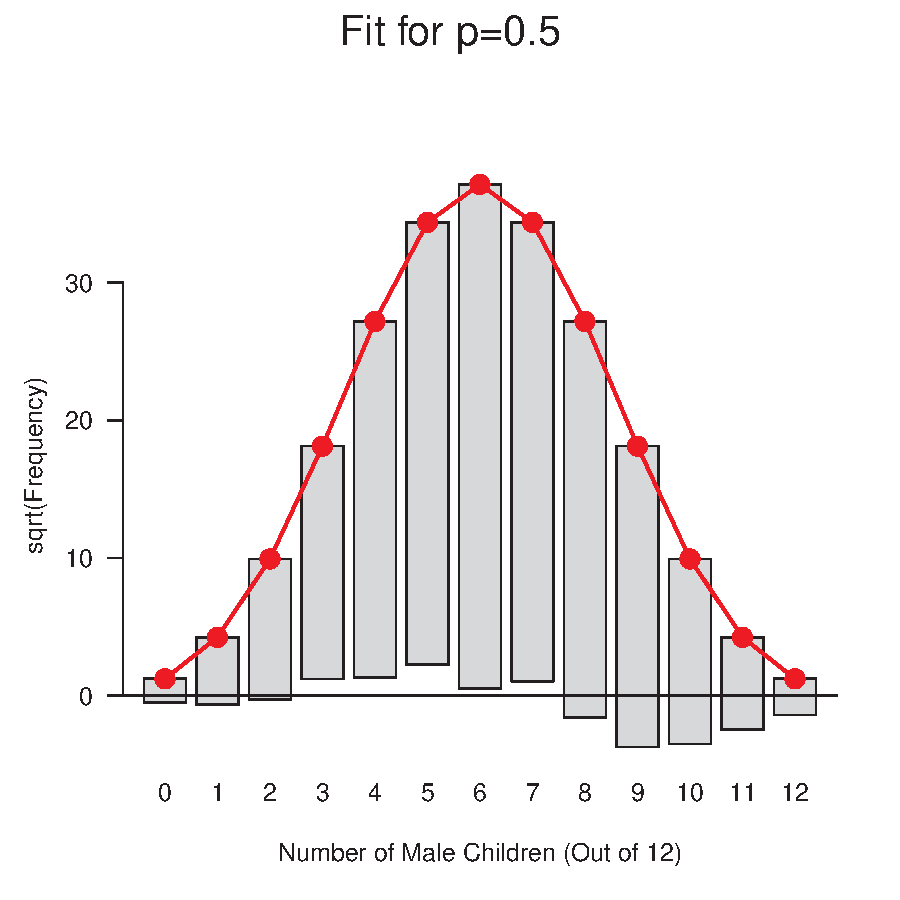
\includegraphics[width=.49\textwidth]{soln/fig/ex3_4c-1} 
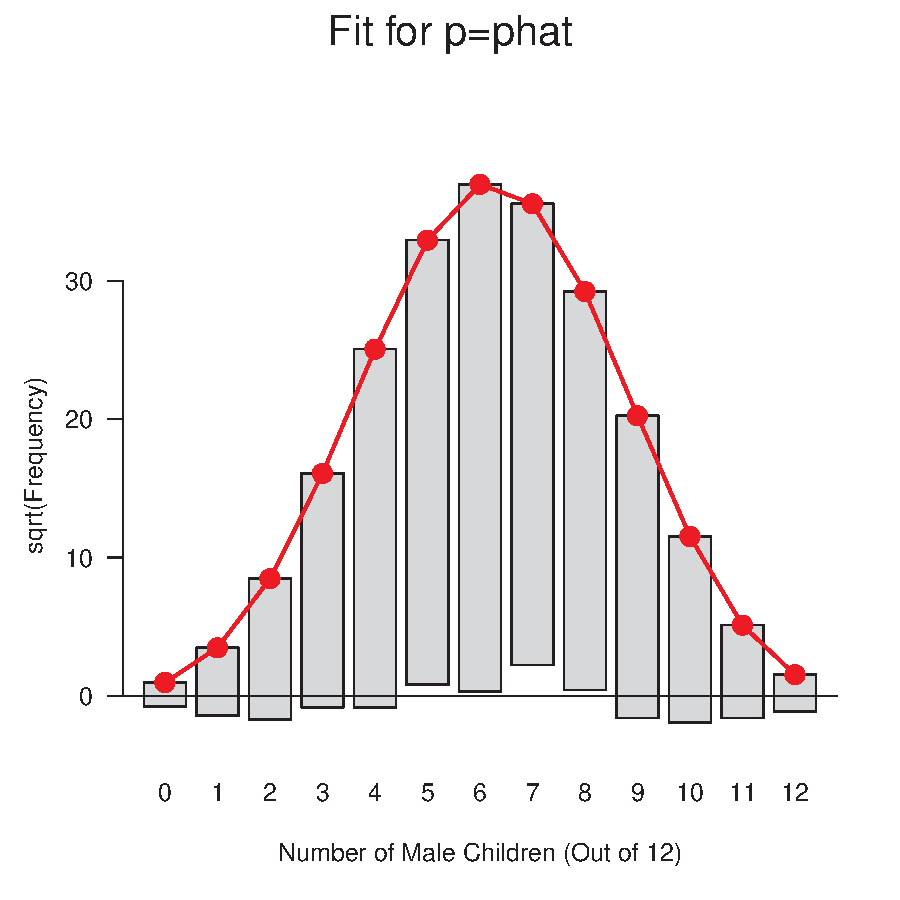
\includegraphics[width=.49\textwidth]{soln/fig/ex3_4c-2} }



\end{knitrout}
    \end{ans}
    
  \end{enumerate*}

  \exercise For the \data{Federalist} data, the examples in \secref{sec:fitdistr} and
  \secref{sec:fitplot} showed the negative binomial to provide an acceptable fit.
  Compare this with the simpler special case of geometric distribution, corresponding
  to $n=1$.
  \begin{enumerate*}
    \item Use \func{goodfit} to fit the geometric distribution. 
    [Hint: use \code{type="nbinomial"}, but specify \code{size=1} as a parameter.]
    \begin{ans}
\begin{knitrout}\footnotesize
\definecolor{shadecolor}{rgb}{0.941, 0.941, 0.941}\color{fgcolor}\begin{kframe}
\begin{alltt}
\hlstd{> }\hlstd{fdfit1} \hlkwb{<-} \hlkwd{goodfit}\hlstd{(Federalist,} \hlkwc{type} \hlstd{=} \hlstr{"binomial"}\hlstd{,} \hlkwc{par} \hlstd{=} \hlkwd{list}\hlstd{(}\hlkwc{size}\hlstd{=}\hlnum{6}\hlstd{))}
\hlstd{> }\hlstd{fdfit1}
\end{alltt}
\begin{verbatim}

Observed and fitted values for binomial distribution
with parameters estimated by `ML' 

 count observed     fitted pearson residual
     0      156 1.3072e+02          2.21074
     1       63 9.6362e+01         -3.39860
     2       29 2.9597e+01         -0.10972
     3        8 4.8483e+00          1.43139
     4        4 4.4673e-01          5.31624
     5        1 2.1954e-02          6.60094
     6        1 4.4953e-04         47.14399
\end{verbatim}
\begin{alltt}
\hlstd{> }\hlstd{fdfit2} \hlkwb{<-} \hlkwd{goodfit}\hlstd{(Federalist,} \hlkwc{type} \hlstd{=} \hlstr{"nbinomial"}\hlstd{,} \hlkwc{par} \hlstd{=} \hlkwd{list}\hlstd{(}\hlkwc{size}\hlstd{=}\hlnum{1}\hlstd{))}
\hlstd{> }\hlstd{fdfit2}
\end{alltt}
\begin{verbatim}

Observed and fitted values for nbinomial distribution
with parameters estimated by `ML with size fixed' 

 count observed    fitted pearson residual
     0      156 158.16590        -0.172219
     1       63  62.68326         0.040006
     2       29  24.84221         0.834194
     3        8   9.84530        -0.588102
     4        4   3.90182         0.049702
     5        1   1.54635        -0.439353
     6        1   0.61284        -0.015044
\end{verbatim}
\end{kframe}
\end{knitrout}
    \end{ans}
    
    \item Compare the negative binomial and the geometric models statistically,
    by a \LR test of the difference between these two models.
    \begin{ans}
\begin{knitrout}\footnotesize
\definecolor{shadecolor}{rgb}{0.941, 0.941, 0.941}\color{fgcolor}\begin{kframe}
\begin{alltt}
\hlstd{> }\hlkwd{summary}\hlstd{(fdfit1)}
\end{alltt}
\begin{verbatim}

	 Goodness-of-fit test for binomial distribution

                    X^2 df   P(> X^2)
Likelihood Ratio 49.026  5 2.1927e-09
\end{verbatim}
\begin{alltt}
\hlstd{> }\hlkwd{summary}\hlstd{(fdfit2)}
\end{alltt}
\begin{verbatim}

	 Goodness-of-fit test for nbinomial distribution

                    X^2 df P(> X^2)
Likelihood Ratio 2.2941  5  0.80713
\end{verbatim}
\end{kframe}
\end{knitrout}
    \end{ans}
    
%\TODO{PC: correct me if I'm wrong, but aren't there models not nested? Wouldn't information criteria therefore be more appropriate?}
    \item Compare the negative binomial and the geometric models visually
    by hanging rootograms or other methods.
    \begin{ans}
    Hanging rootograms:
\begin{knitrout}\footnotesize
\definecolor{shadecolor}{rgb}{0.941, 0.941, 0.941}\color{fgcolor}\begin{kframe}
\begin{alltt}
\hlstd{> }\hlkwd{plot}\hlstd{(fdfit1)}
\hlstd{> }\hlkwd{plot}\hlstd{(fdfit2)}
\end{alltt}
\end{kframe}

\centerline{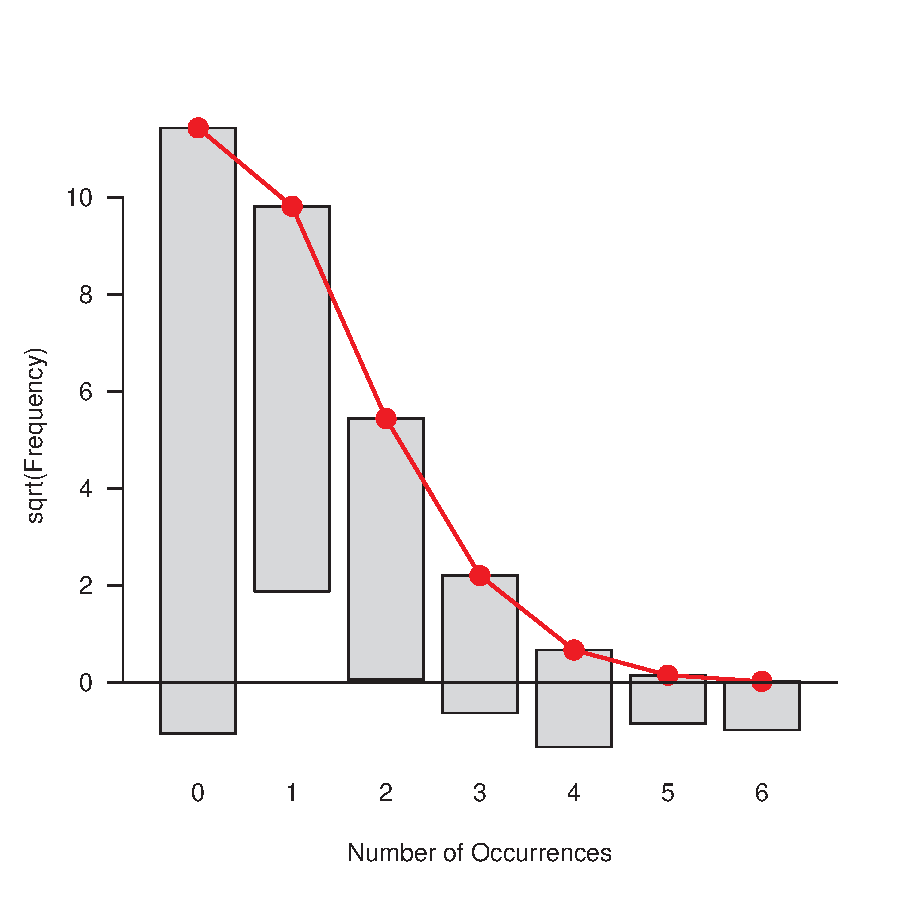
\includegraphics[width=.49\textwidth]{soln/fig/ex3_5c1-1} 
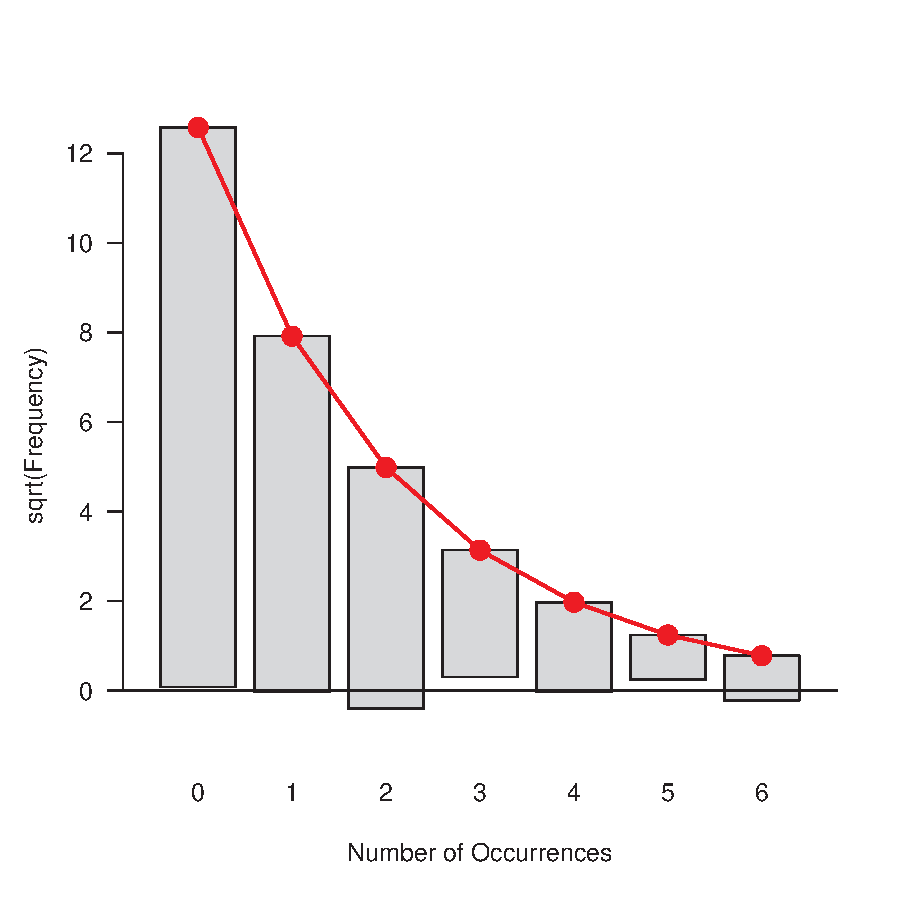
\includegraphics[width=.49\textwidth]{soln/fig/ex3_5c1-2} }



\end{knitrout}
    Distribution-ness plots:
\begin{knitrout}\footnotesize
\definecolor{shadecolor}{rgb}{0.941, 0.941, 0.941}\color{fgcolor}\begin{kframe}
\begin{alltt}
\hlstd{> }\hlkwd{distplot}\hlstd{(Federalist,} \hlkwc{type} \hlstd{=} \hlstr{"binomial"}\hlstd{,} \hlkwc{size}\hlstd{=}\hlnum{6}\hlstd{,} \hlkwc{xlab} \hlstd{=} \hlstr{"Word Count"}\hlstd{)}
\hlstd{> }\hlkwd{distplot}\hlstd{(Federalist,} \hlkwc{type} \hlstd{=} \hlstr{"nbinomial"}\hlstd{,} \hlkwc{size}\hlstd{=}\hlnum{6}\hlstd{,} \hlkwc{xlab} \hlstd{=} \hlstr{"Word Count"}\hlstd{)}
\end{alltt}
\end{kframe}

\centerline{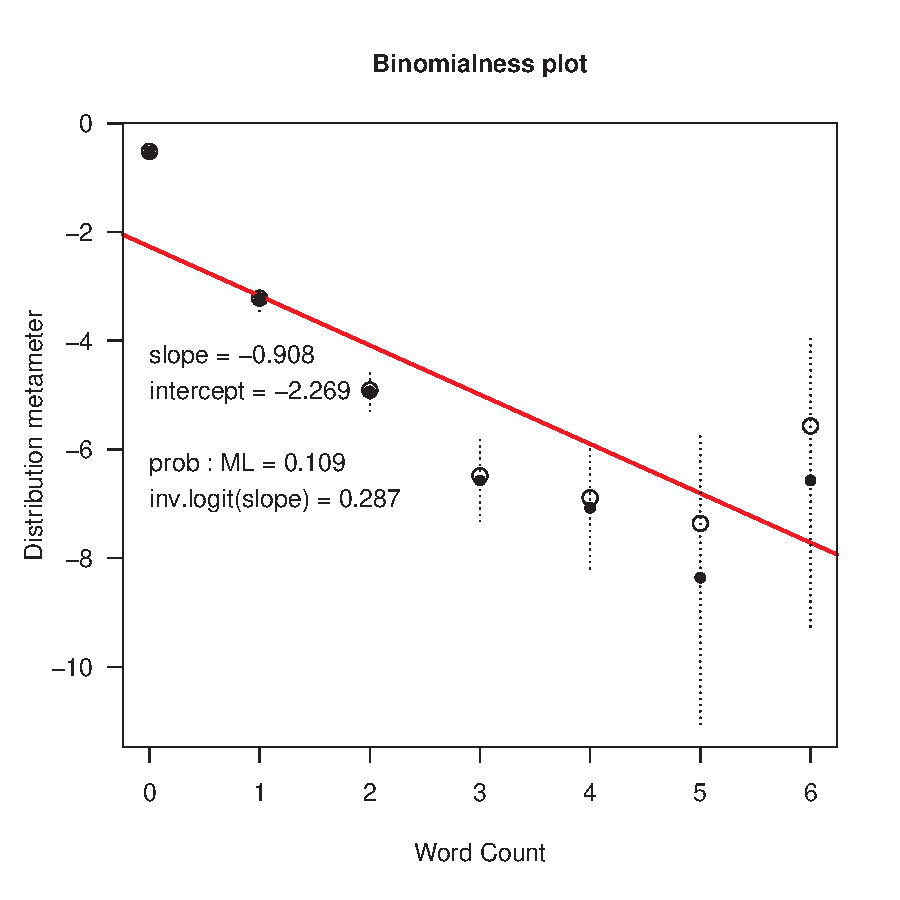
\includegraphics[width=.49\textwidth]{soln/fig/ex3_5c2-1} 
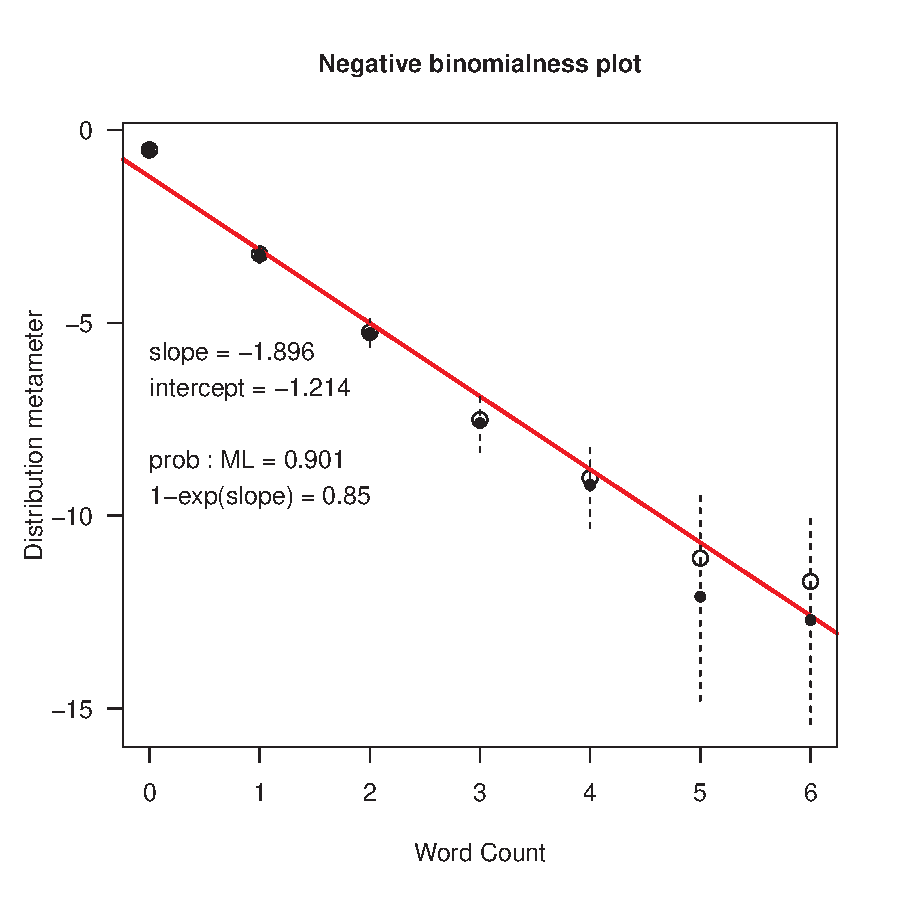
\includegraphics[width=.49\textwidth]{soln/fig/ex3_5c2-2} }



\end{knitrout}
    \end{ans}
    
  \end{enumerate*}

  \exercise \citet[Table 2.4]{MostellerWallace:63} give the frequencies, $n_k$,
  of counts $k = 0, 1, \dots$ of other selected marker words in 247 blocks
  of text known to have been written by Alexander Hamilton.  The data below
  show the occurrences of the word \emph{upon}, that Hamilton used much more than
  did James Madison.
\begin{knitrout}\footnotesize
\definecolor{shadecolor}{rgb}{0.941, 0.941, 0.941}\color{fgcolor}\begin{kframe}
\begin{alltt}
\hlstd{> }\hlstd{count} \hlkwb{<-} \hlnum{0} \hlopt{:} \hlnum{5}
\hlstd{> }\hlstd{Freq} \hlkwb{<-} \hlkwd{c}\hlstd{(}\hlnum{129}\hlstd{,} \hlnum{83}\hlstd{,} \hlnum{20}\hlstd{,} \hlnum{9}\hlstd{,} \hlnum{5}\hlstd{,} \hlnum{1}\hlstd{)}
\end{alltt}
\end{kframe}
\end{knitrout}
  \begin{enumerate*}
    \item Read these data into \R and construct a one-way table of frequencies of counts
    or a matrix or data frame with frequencies in the first column and the corresponding counts in the second column, 
    suitable for use with \func{goodfit}.
    \begin{ans}
    \texttt{goodfit()} requires its first argument to be either a one-way table (from \texttt{xtabs()}),
    or a data.frame with frequencies in the \emph{first} column and the corresponding counts in the second column.  
    Both of the following forms will work.
\begin{knitrout}\footnotesize
\definecolor{shadecolor}{rgb}{0.941, 0.941, 0.941}\color{fgcolor}\begin{kframe}
\begin{alltt}
\hlstd{> }\hlstd{count} \hlkwb{<-} \hlnum{0}\hlopt{:}\hlnum{5}
\hlstd{> }\hlstd{Freq} \hlkwb{<-} \hlkwd{c}\hlstd{(}\hlnum{129}\hlstd{,} \hlnum{83}\hlstd{,} \hlnum{20}\hlstd{,} \hlnum{9}\hlstd{,} \hlnum{5}\hlstd{,} \hlnum{1}\hlstd{)}
\hlstd{> }\hlkwd{sum}\hlstd{(Freq)}  \hlcom{# check N}
\end{alltt}
\begin{verbatim}
[1] 247
\end{verbatim}
\begin{alltt}
\hlstd{> }\hlstd{(Upon} \hlkwb{<-} \hlkwd{data.frame}\hlstd{(Freq, count))}             \hlcom{# as a data.frame}
\end{alltt}
\begin{verbatim}
  Freq count
1  129     0
2   83     1
3   20     2
4    9     3
5    5     4
6    1     5
\end{verbatim}
\begin{alltt}
\hlstd{> }\hlstd{(Upon.tab} \hlkwb{<-} \hlkwd{xtabs}\hlstd{(Freq} \hlopt{~} \hlstd{count,} \hlkwc{data}\hlstd{=Upon))}  \hlcom{# one-way table}
\end{alltt}
\begin{verbatim}
count
  0   1   2   3   4   5 
129  83  20   9   5   1 
\end{verbatim}
\end{kframe}
\end{knitrout}
    \end{ans}
    
    \item Fit and plot the Poisson model for these frequencies.
    \begin{ans}
\begin{knitrout}\footnotesize
\definecolor{shadecolor}{rgb}{0.941, 0.941, 0.941}\color{fgcolor}\begin{kframe}
\begin{alltt}
\hlstd{> }\hlstd{(up0} \hlkwb{<-} \hlkwd{goodfit}\hlstd{(Upon,} \hlkwc{type}\hlstd{=}\hlstr{"poisson"}\hlstd{))}
\end{alltt}
\begin{verbatim}

Observed and fitted values for poisson distribution
with parameters estimated by `ML' 

 count observed    fitted pearson residual
     0      129 121.61816          0.66937
     1       83  86.16671         -0.34115
     2       20  30.52465         -1.90494
     3        9   7.20892          0.66708
     4        5   1.27688          3.29481
     5        1   0.18094          1.75800
\end{verbatim}
\begin{alltt}
\hlstd{> }\hlkwd{summary}\hlstd{(up0)}
\end{alltt}
\begin{verbatim}

	 Goodness-of-fit test for poisson distribution

                    X^2 df P(> X^2)
Likelihood Ratio 13.139  4 0.010617
\end{verbatim}
\begin{alltt}
\hlstd{> }\hlkwd{plot}\hlstd{(up0)}
\end{alltt}
\end{kframe}

\centerline{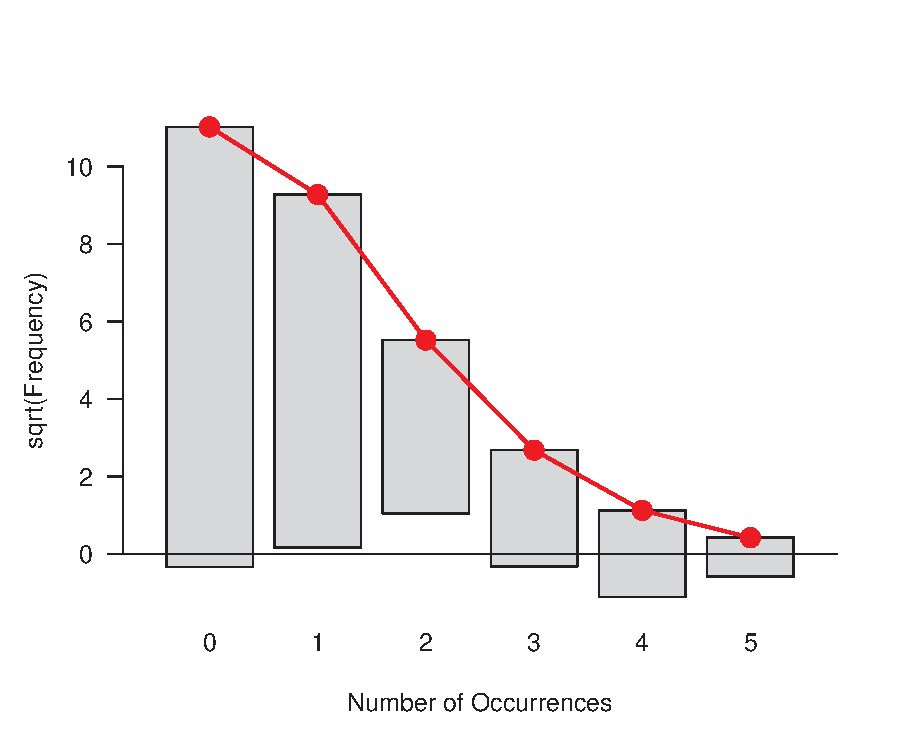
\includegraphics[width=.5\textwidth]{soln/fig/ex3_6b-1} }



\end{knitrout}
    \end{ans}
    
    \item Fit and plot the negative binomial model for these frequencies.
    \begin{ans}
\begin{knitrout}\footnotesize
\definecolor{shadecolor}{rgb}{0.941, 0.941, 0.941}\color{fgcolor}\begin{kframe}
\begin{alltt}
\hlstd{> }\hlstd{(up1} \hlkwb{<-} \hlkwd{goodfit}\hlstd{(Upon,} \hlkwc{type}\hlstd{=}\hlstr{"nbinomial"}\hlstd{))}
\end{alltt}
\begin{verbatim}

Observed and fitted values for nbinomial distribution
with parameters estimated by `ML' 

 count observed    fitted pearson residual
     0      129 131.65936        -0.231767
     1       83  73.89421         1.059285
     2       20  28.41547        -1.578705
     3        9   9.25319        -0.083233
     4        5   2.74068         1.364738
     5        1   0.76332        -0.036432
\end{verbatim}
\begin{alltt}
\hlstd{> }\hlkwd{summary}\hlstd{(up1)}
\end{alltt}
\begin{verbatim}

	 Goodness-of-fit test for nbinomial distribution

                    X^2 df P(> X^2)
Likelihood Ratio 6.0306  3  0.11013
\end{verbatim}
\begin{alltt}
\hlstd{> }\hlkwd{plot}\hlstd{(up1)}
\end{alltt}
\end{kframe}

\centerline{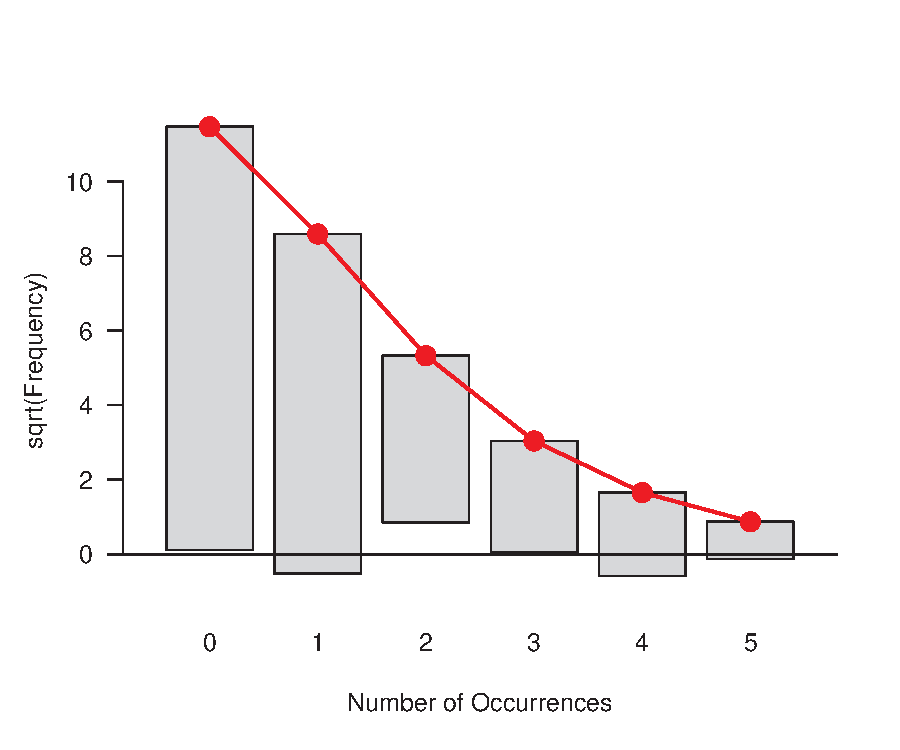
\includegraphics[width=.5\textwidth]{soln/fig/ex3_6c-1} }



\end{knitrout}
    \end{ans}
    
    \item What do you conclude?
    \begin{ans}
    The negative binomial model fits better than the Poisson.
    \end{ans}
    
  \end{enumerate*}

  \exercise The data frame \data{Geissler} in the \Rpackage{vcdExtra} contains the complete data from Geissler's \citeyearpar{Geissler:1889} tabulation of family sex composition in Saxony.  The table below gives the number of boys in families of size 11.

% latex table generated in R 3.0.1 by xtable 1.7-2 package
% Tue Dec 17 10:15:54 2013
%\begin{table}[ht]
%\centering
\begin{tabular}{r|rrrrrrrrrrrr}
%  \hline
% & 1 & 2 & 3 & 4 & 5 & 6 & 7 & 8 & 9 & 10 & 11 & 12 \\
  \hline
boys &   0 &   1 &   2 &   3 &   4 &   5 &   6 &   7 &   8 &   9 &  10 &  11 \\
  Freq &   8 &  72 & 275 & 837 & 1,540 & 2,161 & 2,310 & 1,801 & 1,077 & 492 &  93 &  24 \\
   \hline
\end{tabular}
%\end{table}
% the table is better

  \begin{enumerate*}
    \item Read these data into \R.
    \begin{ans}
    See Exercise 2.6, which calculates \texttt{sax11} in the form of a data frame.
    \end{ans}

    \item Following \exref{ex:saxfit}, use \func{goodfit} to fit the binomial model and plot the
    results.  Is there an indication that the binomial does not fit these data?
    \begin{ans}
    The binomial distribution fits badly, where the extremes are under-fitted, and the middle
    values are over-fitted.
\begin{knitrout}\footnotesize
\definecolor{shadecolor}{rgb}{0.941, 0.941, 0.941}\color{fgcolor}\begin{kframe}
\begin{alltt}
\hlstd{> }\hlstd{sax11.tab} \hlkwb{<-} \hlkwd{xtabs}\hlstd{(Freq} \hlopt{~} \hlstd{boys,} \hlkwc{data}\hlstd{=sax11)}
\hlstd{> }\hlkwd{goodfit}\hlstd{(sax11.tab,} \hlkwc{type}\hlstd{=}\hlstr{"binomial"}\hlstd{,} \hlkwc{par}\hlstd{=}\hlkwd{list}\hlstd{(}\hlkwc{size}\hlstd{=}\hlnum{11}\hlstd{))}
\end{alltt}
\begin{verbatim}

Observed and fitted values for binomial distribution
with parameters estimated by `ML' 

 count observed    fitted pearson residual
     0        8    3.5616           2.3518
     1       72   41.9479           4.6400
     2      275  224.5724           3.3650
     3      837  721.3629           4.3055
     4     1540 1544.7559          -0.1210
     5     2161 2315.6023          -3.2128
     6     2310 2479.3627          -3.4013
     7     1801 1896.2173          -2.1866
     8     1077 1015.1593           1.9409
     9      492  362.3173           6.8130
    10       93   77.5881           1.7497
    11       24    7.5523           5.9850
\end{verbatim}
\begin{alltt}
\hlstd{> }\hlkwd{summary}\hlstd{(}\hlkwd{goodfit}\hlstd{(sax11.tab,} \hlkwc{type}\hlstd{=}\hlstr{"binomial"}\hlstd{,} \hlkwc{par}\hlstd{=}\hlkwd{list}\hlstd{(}\hlkwc{size}\hlstd{=}\hlnum{11}\hlstd{)))}
\end{alltt}
\begin{verbatim}

	 Goodness-of-fit test for binomial distribution

                    X^2 df   P(> X^2)
Likelihood Ratio 148.09 10 9.2126e-27
\end{verbatim}
\end{kframe}
\end{knitrout}
    \end{ans}
    
    \item Diagnose the form of the distribution using the methods described in \secref{sec:discrete-ord}.
    \begin{ans}
    The Ord plot indicates that the closest distribution according to its heuristics is the binomial;
    the binomialness distribution plot, however, shows this is not an acceptable model, as was also
    seen in the text for families of size 12.
\begin{knitrout}\footnotesize
\definecolor{shadecolor}{rgb}{0.941, 0.941, 0.941}\color{fgcolor}\begin{kframe}
\begin{alltt}
\hlstd{> }\hlkwd{Ord_plot}\hlstd{(sax11.tab)}
\hlstd{> }\hlkwd{distplot}\hlstd{(sax11.tab,} \hlkwc{type}\hlstd{=}\hlstr{"binomial"}\hlstd{,} \hlkwc{size}\hlstd{=}\hlnum{11}\hlstd{)}
\end{alltt}
\end{kframe}

\centerline{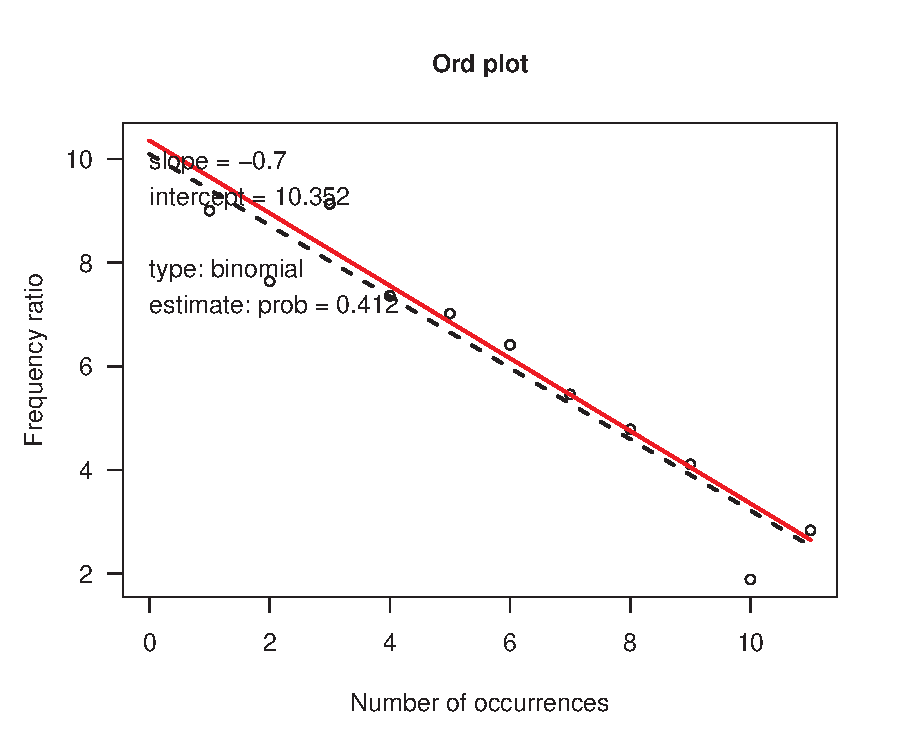
\includegraphics[width=.5\textwidth]{soln/fig/ex3_7c-1} 
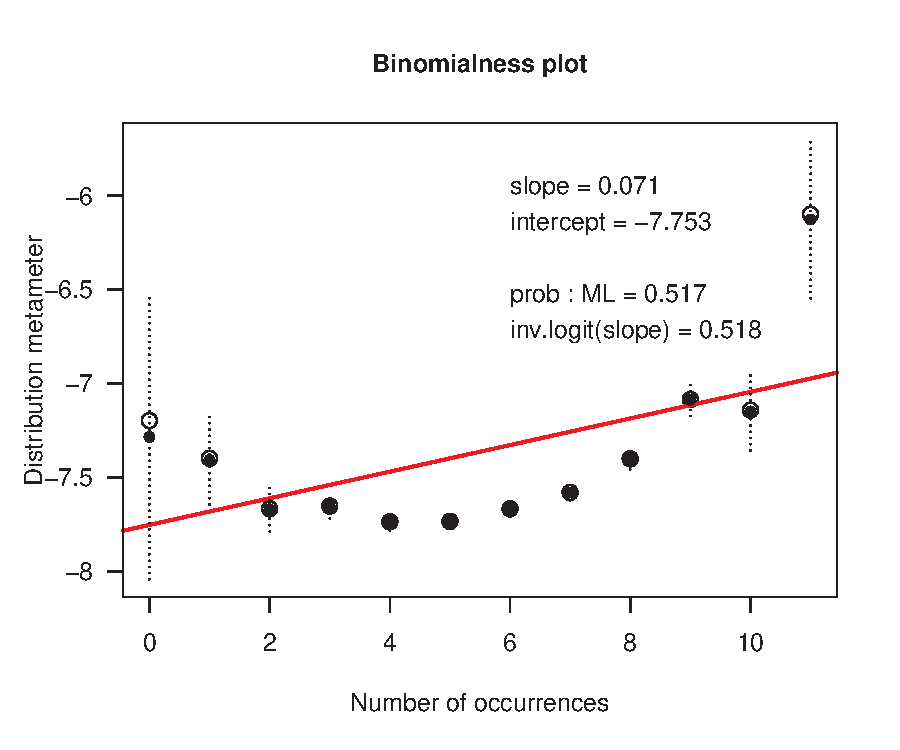
\includegraphics[width=.5\textwidth]{soln/fig/ex3_7c-2} }



\end{knitrout}
    \end{ans}
    
    \item Try fitting the negative binomial distribution, and use \func{distplot} to diagnose
    whether the negative binomial is a reasonable fit. \TODO{Something wrong here.}
    \begin{ans}
\begin{knitrout}\footnotesize
\definecolor{shadecolor}{rgb}{0.941, 0.941, 0.941}\color{fgcolor}\begin{kframe}
\begin{alltt}
\hlstd{> }\hlkwd{goodfit}\hlstd{(sax11.tab,} \hlkwc{type}\hlstd{=}\hlstr{"nbinomial"}\hlstd{,} \hlkwc{par}\hlstd{=}\hlkwd{list}\hlstd{(}\hlkwc{size}\hlstd{=}\hlnum{11}\hlstd{))}
\end{alltt}
\begin{verbatim}

Observed and fitted values for nbinomial distribution
with parameters estimated by `ML with size fixed' 

 count observed  fitted pearson residual
     0        8  109.12          -9.6801
     1       72  409.11         -16.6667
     2      275  836.63         -19.4171
     3      837 1235.67         -11.3414
     4     1540 1474.07           1.7171
     5     2161 1507.26          16.8389
     6     2310 1369.95          25.3981
     7     1801 1133.97          19.8082
     8     1077  869.62           7.0323
     9      492  625.73          -5.3462
    10       93  426.55         -16.1500
    11       24  277.55         -25.3999
\end{verbatim}
\end{kframe}
\end{knitrout}
    \end{ans}
    
  \end{enumerate*}

  \exercise The data frame \data{Bundesliga} gives a similar data set to that for UK soccer scores
  (\data{UKSoccer})
  examined in \exref{ex:soccer}, but over a wide range of years.  The following lines calculate
  a two-way table, \code{BL1995}, of home-team and away-team goals
  for the 306 games in the year 1995.
\begin{knitrout}\footnotesize
\definecolor{shadecolor}{rgb}{0.941, 0.941, 0.941}\color{fgcolor}\begin{kframe}
\begin{alltt}
\hlstd{> }\hlkwd{data}\hlstd{(}\hlstr{"Bundesliga"}\hlstd{,} \hlkwc{package} \hlstd{=} \hlstr{"vcd"}\hlstd{)}
\hlstd{> }\hlstd{BL1995} \hlkwb{<-} \hlkwd{xtabs}\hlstd{(}\hlopt{~} \hlstd{HomeGoals} \hlopt{+} \hlstd{AwayGoals,} \hlkwc{data} \hlstd{= Bundesliga,}
\hlstd{+ }                \hlkwc{subset} \hlstd{= (Year} \hlopt{==} \hlnum{1995}\hlstd{))}
\hlstd{> }\hlstd{BL1995}
\end{alltt}
\begin{verbatim}
         AwayGoals
HomeGoals  0  1  2  3  4  5  6
        0 26 16 13  5  0  1  0
        1 19 58 20  5  4  0  1
        2 27 23 20  5  1  1  1
        3 14 11 10  4  2  0  0
        4  3  5  3  0  0  0  0
        5  4  1  0  1  0  0  0
        6  1  0  0  1  0  0  0
\end{verbatim}
\end{kframe}
\end{knitrout}
  \begin{enumerate*}
    \item As in , find the one-way distributions of \code{HomeGoals},
    \code{AwayGoals}, and \code{TotalGoals = HomeGoals + AwayGoals}.
    \begin{ans}
    There are several ways to do this, but as illustrated in the text for \exref{ex:soccer}, 
    create the one-way variables in a \code{data.frame}, and then use \func{xtabs}
    to get their marginal distributions.
\begin{knitrout}\footnotesize
\definecolor{shadecolor}{rgb}{0.941, 0.941, 0.941}\color{fgcolor}\begin{kframe}
\begin{alltt}
\hlstd{> }\hlstd{BL.df} \hlkwb{<-} \hlkwd{as.data.frame}\hlstd{(BL1995,} \hlkwc{stringsASFactors}\hlstd{=}\hlnum{FALSE}\hlstd{)}
\hlstd{> }\hlstd{BL.df} \hlkwb{<-} \hlkwd{within}\hlstd{(BL.df, \{}
\hlstd{+ }  \hlstd{HomeGoals} \hlkwb{<-} \hlkwd{as.numeric}\hlstd{(HomeGoals)}
\hlstd{+ }  \hlstd{AwayGoals} \hlkwb{<-} \hlkwd{as.numeric}\hlstd{(AwayGoals)}
\hlstd{+ }  \hlstd{TotalGoals} \hlkwb{<-} \hlstd{HomeGoals} \hlopt{+} \hlstd{AwayGoals}
\hlstd{+ }  \hlstd{\})}
\hlstd{> }   \hlcom{# marginal distributions}
\hlstd{> }\hlstd{(BL.home} \hlkwb{<-} \hlkwd{xtabs}\hlstd{(Freq} \hlopt{~} \hlstd{HomeGoals,} \hlkwc{data}\hlstd{=BL.df))}
\end{alltt}
\begin{verbatim}
HomeGoals
  1   2   3   4   5   6   7 
 61 107  78  41  11   6   2 
\end{verbatim}
\begin{alltt}
\hlstd{> }\hlstd{(BL.away} \hlkwb{<-} \hlkwd{xtabs}\hlstd{(Freq} \hlopt{~} \hlstd{AwayGoals,} \hlkwc{data}\hlstd{=BL.df))}
\end{alltt}
\begin{verbatim}
AwayGoals
  1   2   3   4   5   6   7 
 94 114  66  21   7   2   2 
\end{verbatim}
\begin{alltt}
\hlstd{> }\hlstd{(BL.total} \hlkwb{<-} \hlkwd{xtabs}\hlstd{(Freq} \hlopt{~} \hlstd{TotalGoals,} \hlkwc{data}\hlstd{=BL.df))}
\end{alltt}
\begin{verbatim}
TotalGoals
 2  3  4  5  6  7  8  9 10 11 12 13 14 
26 35 98 62 39 29 10  4  2  1  0  0  0 
\end{verbatim}
\end{kframe}
\end{knitrout}
    \end{ans}
    
    \item Use \func{goodfit} to fit and plot the Poisson distribution to each of these.  Does the
    Poisson seem to provide a reasonable fit?
    \begin{ans}
    The Poisson distribution has a bad fit for all of these.
\begin{knitrout}\footnotesize
\definecolor{shadecolor}{rgb}{0.941, 0.941, 0.941}\color{fgcolor}\begin{kframe}
\begin{alltt}
\hlstd{> }\hlkwd{summary}\hlstd{(}\hlkwd{goodfit}\hlstd{(BL.home))}
\end{alltt}
\begin{verbatim}

	 Goodness-of-fit test for poisson distribution

                    X^2 df   P(> X^2)
Likelihood Ratio 70.722  5 7.2516e-14
\end{verbatim}
\begin{alltt}
\hlstd{> }\hlkwd{summary}\hlstd{(}\hlkwd{goodfit}\hlstd{(BL.away))}
\end{alltt}
\begin{verbatim}

	 Goodness-of-fit test for poisson distribution

                    X^2 df   P(> X^2)
Likelihood Ratio 97.973  5 1.4131e-19
\end{verbatim}
\begin{alltt}
\hlstd{> }\hlkwd{summary}\hlstd{(}\hlkwd{goodfit}\hlstd{(BL.total))}
\end{alltt}
\begin{verbatim}

	 Goodness-of-fit test for poisson distribution

                    X^2 df   P(> X^2)
Likelihood Ratio 72.558  8 1.5185e-12
\end{verbatim}
\end{kframe}
\end{knitrout}
    \end{ans}
    
    \item Use \func{distplot} to assess fit of the Poisson distribution.
    \begin{ans}
    The distribution plots for home goals looks better than that for away goals, which shows
    a systematic departure from the red line.
\begin{knitrout}\footnotesize
\definecolor{shadecolor}{rgb}{0.941, 0.941, 0.941}\color{fgcolor}\begin{kframe}
\begin{alltt}
\hlstd{> }\hlkwd{distplot}\hlstd{(BL.home,} \hlkwc{xlab}\hlstd{=}\hlstr{"Number of home goals"}\hlstd{)}
\hlstd{> }\hlkwd{distplot}\hlstd{(BL.away,} \hlkwc{xlab}\hlstd{=}\hlstr{"Number of away goals"}\hlstd{)}
\end{alltt}
\end{kframe}

\centerline{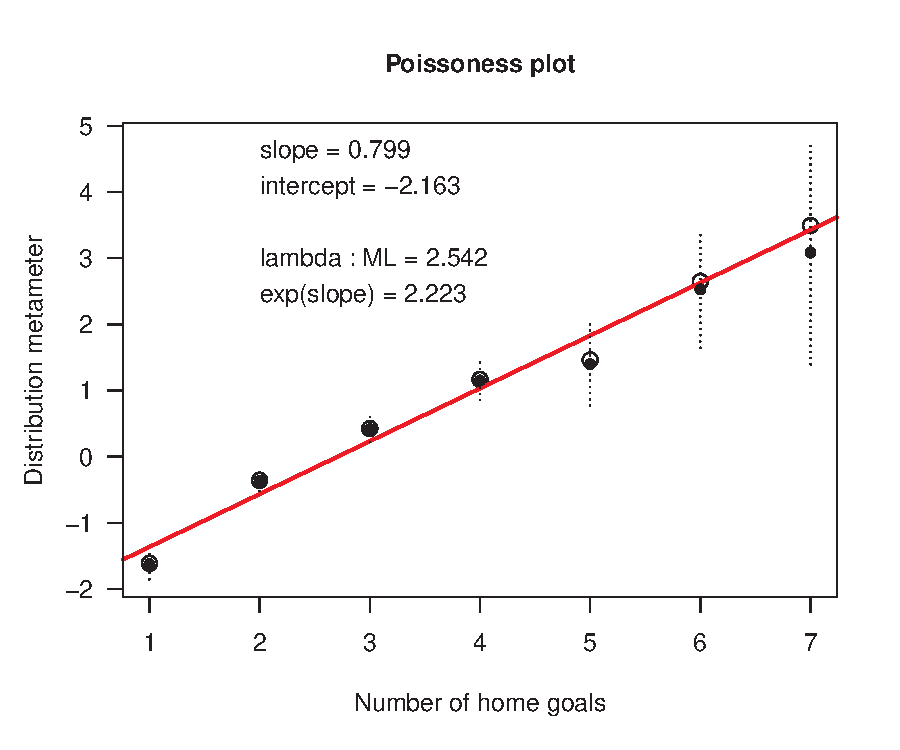
\includegraphics[width=.5\textwidth]{soln/fig/ex3_8c-1} 
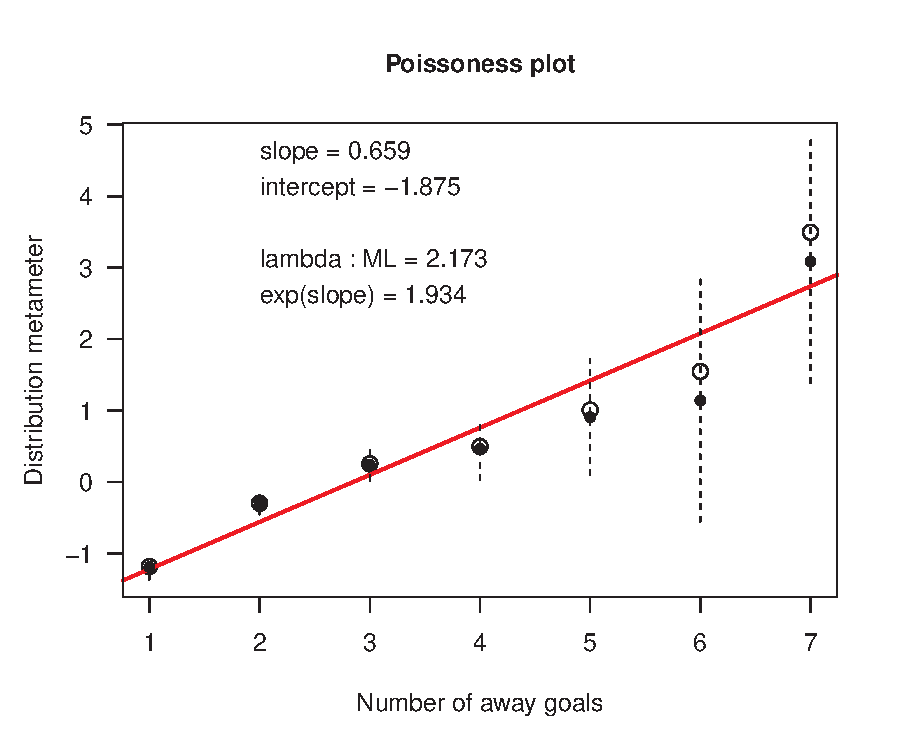
\includegraphics[width=.5\textwidth]{soln/fig/ex3_8c-2} }



\end{knitrout}
    \end{ans}
    
    \item What circumstances of scoring goals in soccer might cause these distributions to
    deviate from Poisson distributions?
    \begin{ans}
    The Poisson distribution relies on (a) independent events with (b) constant probabilities. The probability of scoring a goal 
    is almost certainly not constant over all pairs of teams.
    \end{ans}
    
  \end{enumerate*}

  \exercise\exhard
  Repeat the exercise above, this time using the data for all years in which there was
  the standard number (306) of games, that is for \code{Year>1965}, tabulated as shown below.
\begin{knitrout}\footnotesize
\definecolor{shadecolor}{rgb}{0.941, 0.941, 0.941}\color{fgcolor}\begin{kframe}
\begin{alltt}
\hlstd{> }\hlstd{BL} \hlkwb{<-} \hlkwd{xtabs}\hlstd{(}\hlopt{~} \hlstd{HomeGoals} \hlopt{+} \hlstd{AwayGoals,} \hlkwc{data} \hlstd{= Bundesliga,}
\hlstd{+ }            \hlkwc{subset} \hlstd{= (Year} \hlopt{>} \hlnum{1965}\hlstd{))}
\hlstd{> }\hlstd{BL}
\end{alltt}
\begin{verbatim}
         AwayGoals
HomeGoals    0    1    2    3    4    5    6    7    8    9
       0   868  590  458  206   88   22   12    2    0    0
       1  1049 1550  589  360  121   34    8    6    1    1
       2  1039 1144  810  228   95   26   10    2    1    0
       3   712  793  392  187   43    8    5    2    0    0
       4   346  388  245   73   26    2    3    0    0    0
       5   128  164  106   34    2    2    1    0    0    0
       6    61   63   38   10    0    2    0    0    0    0
       7    20   16   12    4    3    0    0    0    0    0
       8     2    4    3    0    1    0    0    0    0    0
       9     2    2    1    0    0    0    0    0    0    0
       10    2    0    0    0    0    0    0    0    0    0
       11    1    2    0    0    0    0    0    0    0    0
       12    1    0    0    0    0    0    0    0    0    0
\end{verbatim}
\end{kframe}
\end{knitrout}
    \begin{ans}
    The steps are similar to those in the previous problem, but now there are more years, and the
    range of both home goals and away goals is larger.
    \end{ans}


\exercise Using the data \data{CyclingDeaths} introduced in \exref{ex:cyclists1}
and the one-way frequency table \code{CyclingDeaths.tab = table(CyclingDeaths$deaths)}, %$
  \begin{enumerate*}
    \item Make a sensible plot of the number of deaths over time. For extra credit,
    add a smoothed curve (e.g., using \code{lines(lowess(...))}).
    \begin{ans}
    The number of deaths in a given fortnight are discrete, taking values \code{0:3}.
    A barplot, using \code{plot(deaths ~ date, type="h", data=CyclingDeaths)} is one
    option.  Perhaps slightly better is to jitter the number of deaths.
\begin{knitrout}\footnotesize
\definecolor{shadecolor}{rgb}{0.941, 0.941, 0.941}\color{fgcolor}\begin{kframe}
\begin{alltt}
\hlstd{> }\hlkwd{data}\hlstd{(}\hlstr{"CyclingDeaths"}\hlstd{,} \hlkwc{package}\hlstd{=}\hlstr{"vcdExtra"}\hlstd{)}
\hlstd{> }\hlstd{CyclingDeaths.tab} \hlkwb{<-} \hlkwd{table}\hlstd{(CyclingDeaths}\hlopt{$}\hlstd{deaths)}
\hlstd{> }\hlkwd{plot}\hlstd{(}\hlkwd{jitter}\hlstd{(deaths)} \hlopt{~} \hlstd{date,} \hlkwc{data}\hlstd{=CyclingDeaths)}
\hlstd{> }\hlkwd{with}\hlstd{(CyclingDeaths, \{}\hlkwd{lines}\hlstd{(}\hlkwd{lowess}\hlstd{(date, deaths),} \hlkwc{lwd}\hlstd{=}\hlnum{3}\hlstd{,} \hlkwc{col}\hlstd{=}\hlstr{"blue"}\hlstd{)\})}
\end{alltt}
\end{kframe}

\centerline{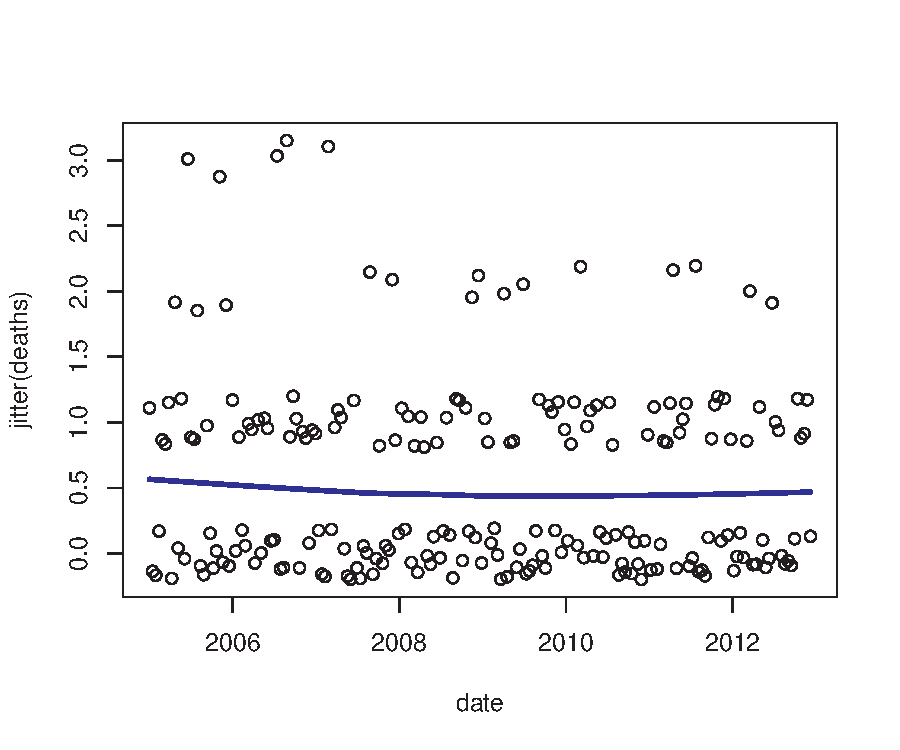
\includegraphics[width=.5\textwidth]{soln/fig/ex3_10a-1} }



\end{knitrout}
    \end{ans}
    
    \item Test the goodness of fit of the table \code{CyclingDeaths.tab} to
    a Poisson distribution statistically using \func{goodfit}.
    \begin{ans}
\begin{knitrout}\footnotesize
\definecolor{shadecolor}{rgb}{0.941, 0.941, 0.941}\color{fgcolor}\begin{kframe}
\begin{alltt}
\hlstd{> }\hlstd{gf} \hlkwb{<-} \hlkwd{goodfit}\hlstd{(CyclingDeaths.tab)}
\hlstd{> }\hlstd{gf}
\end{alltt}
\begin{verbatim}

Observed and fitted values for poisson distribution
with parameters estimated by `ML' 

 count observed   fitted pearson residual
     0      114 117.9464         -0.36338
     1       75  66.9119          0.98877
     2       14  18.9798         -1.14306
     3        5   3.5891          0.41084
\end{verbatim}
\begin{alltt}
\hlstd{> }\hlkwd{summary}\hlstd{(gf)}
\end{alltt}
\begin{verbatim}

	 Goodness-of-fit test for poisson distribution

                    X^2 df P(> X^2)
Likelihood Ratio 4.1517  2  0.12545
\end{verbatim}
\end{kframe}
\end{knitrout}
    \end{ans}
    
    \item Continue this analysis using a \func{rootogram} and \func{distplot}.
    \begin{ans}
\begin{knitrout}\footnotesize
\definecolor{shadecolor}{rgb}{0.941, 0.941, 0.941}\color{fgcolor}\begin{kframe}
\begin{alltt}
\hlstd{> }\hlkwd{plot}\hlstd{(gf,} \hlkwc{xlab}\hlstd{=}\hlstr{"Number of Deaths"}\hlstd{)}
\hlstd{> }\hlkwd{distplot}\hlstd{(CyclingDeaths.tab)}
\end{alltt}
\end{kframe}

\centerline{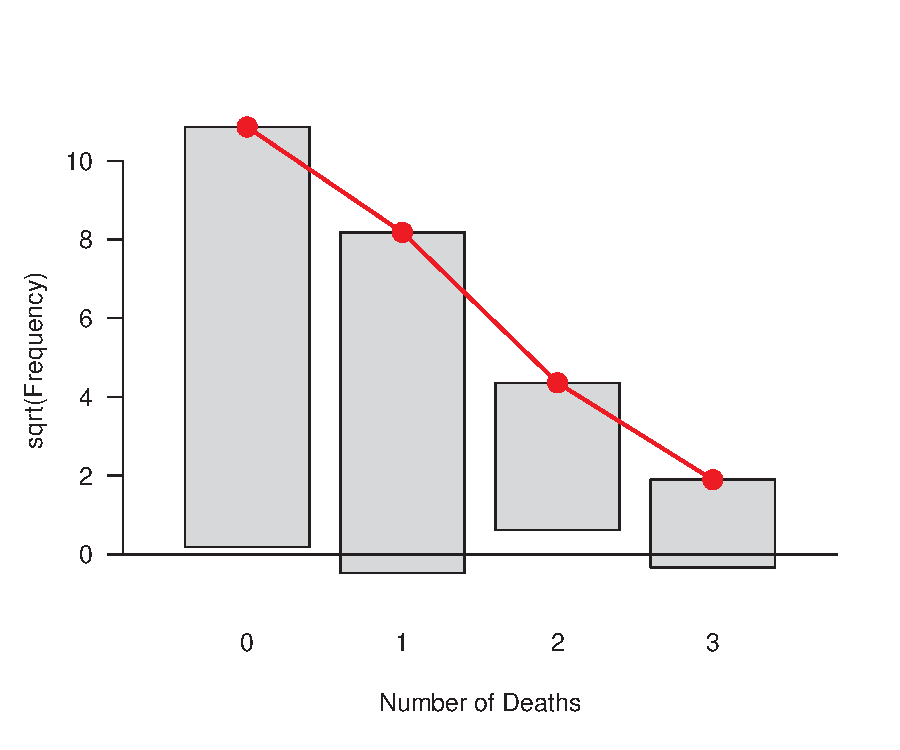
\includegraphics[width=.5\textwidth]{soln/fig/ex3_10c-1} 
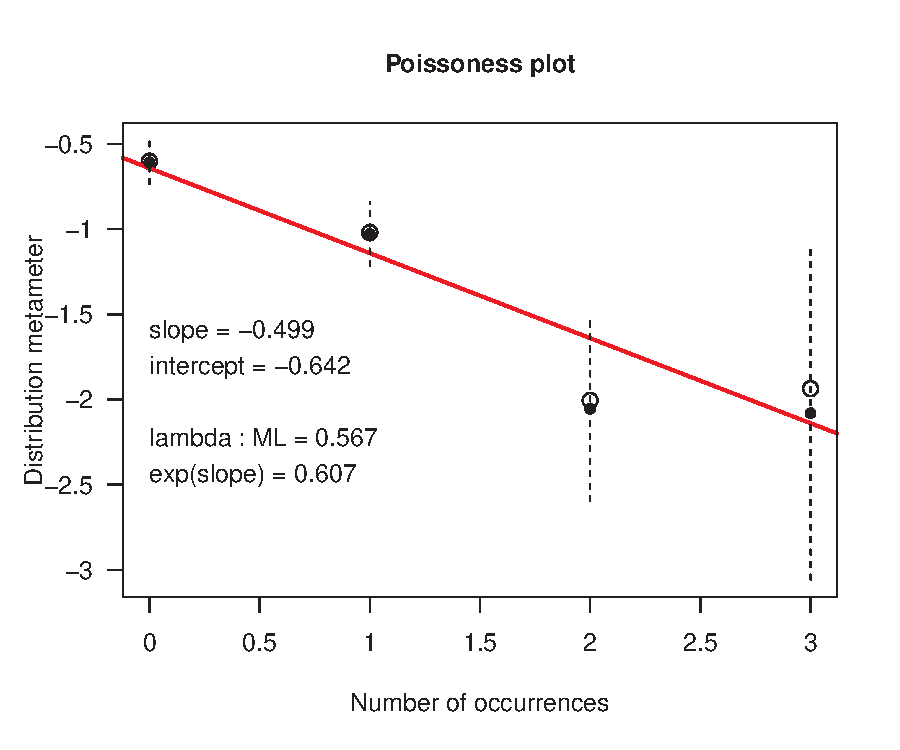
\includegraphics[width=.5\textwidth]{soln/fig/ex3_10c-2} }



\end{knitrout}
    \end{ans}
    
    \item Write a one-paragraph summary of the results of these analyses and your
    conclusions.
    \begin{ans}
    \end{ans}
    
  \end{enumerate*}


\exercise\exhard
  The one-way table, \data{Depends}, in \pkg{vcdExtra} and shown below gives the frequency
  distribution of the number of dependencies declared in $4,983$ \R packages
  maintained on the CRAN distribution network on January 17, 2014. That is, there were 986
  packages that had no dependencies, $1,347$ packages that depended on one other package, $\dots$
  up to 2 packages that depended on 14 other packages.

% \TODO{Perhaps promote this table to an introductory
% example, leaving analysis to this exercise.}
% latex table generated in R 3.0.1 by xtable 1.7-1 package
% Fri Jan 17 09:50:19 2014
\begin{table}[ht]
\centering
\begin{tabular}{r|rrrrrrrrrrrrrrr}
  \hline
Depends & 0 & 1 & 2 & 3 & 4 & 5 & 6 & 7 & 8 & 9 & 10 & 11 & 12 & 13 & 14 \\
  \hline
\# Pkgs & 986 & 1,347 & 993 & 685 & 375 & 298 & 155 &  65 &  32 &  19 &   9 &   4 &   9 &   4 &   2 \\
   \hline
\end{tabular}
\end{table}

    \begin{enumerate*}
      \item Make a bar plot of this distribution.
      \begin{ans}
\begin{knitrout}\footnotesize
\definecolor{shadecolor}{rgb}{0.941, 0.941, 0.941}\color{fgcolor}\begin{kframe}
\begin{alltt}
\hlstd{> }\hlkwd{data}\hlstd{(}\hlstr{"Depends"}\hlstd{,} \hlkwc{package}\hlstd{=}\hlstr{"vcdExtra"}\hlstd{)}
\hlstd{> }\hlkwd{plot}\hlstd{(Depends,} \hlkwc{xlab}\hlstd{=}\hlstr{"Number of Dependencies"}\hlstd{,} \hlkwc{ylab}\hlstd{=}\hlstr{"Number of R Packages"}\hlstd{,} \hlkwc{lwd}\hlstd{=}\hlnum{8}\hlstd{)}
\end{alltt}
\end{kframe}

\centerline{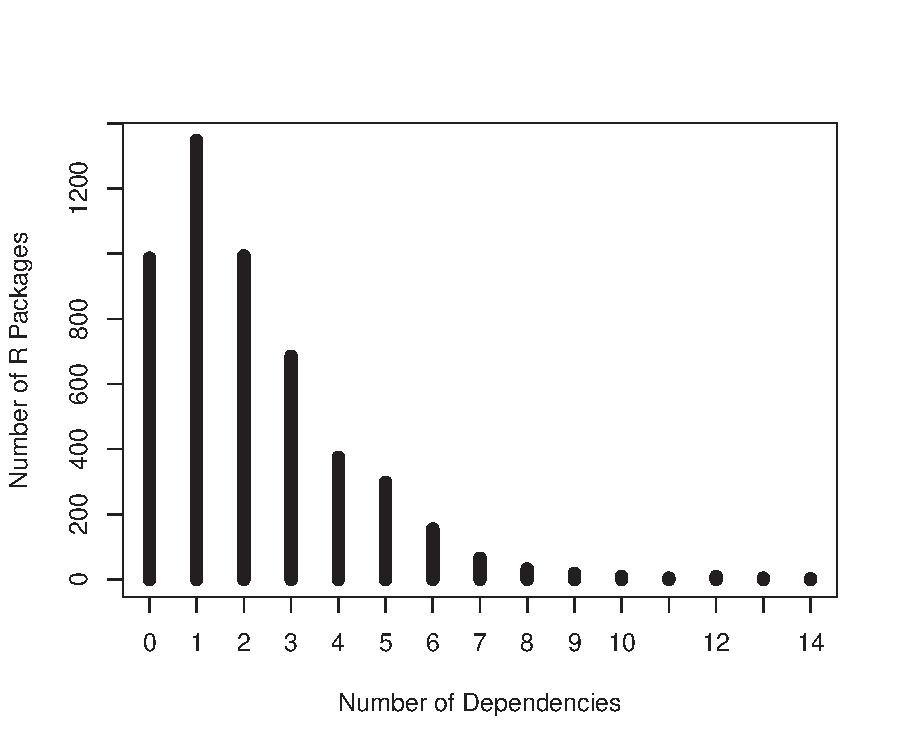
\includegraphics[width=.5\textwidth]{soln/fig/ex3_11a-1} }



\end{knitrout}
      \end{ans}
      
      \item Use \func{Ord\_plot} to see if this method can diagnose the form of the distribution.
      \begin{ans}
      This turns out to be a case where the Ord plot method, as implemented in
      \func{Ord\_plot} does not determine the form of the distribution.  According to 
      \tabref{tab:ordparm}, the log series distribution is the only one with positive
      slope $b$ and negative intercept $a$, but this requires $a = -b$. 
      %\TODO{Is this a bug in Ord\_plot?}
\begin{knitrout}\footnotesize
\definecolor{shadecolor}{rgb}{0.941, 0.941, 0.941}\color{fgcolor}\begin{kframe}
\begin{alltt}
\hlstd{> }\hlkwd{Ord_plot}\hlstd{(Depends)}
\end{alltt}
\end{kframe}

\centerline{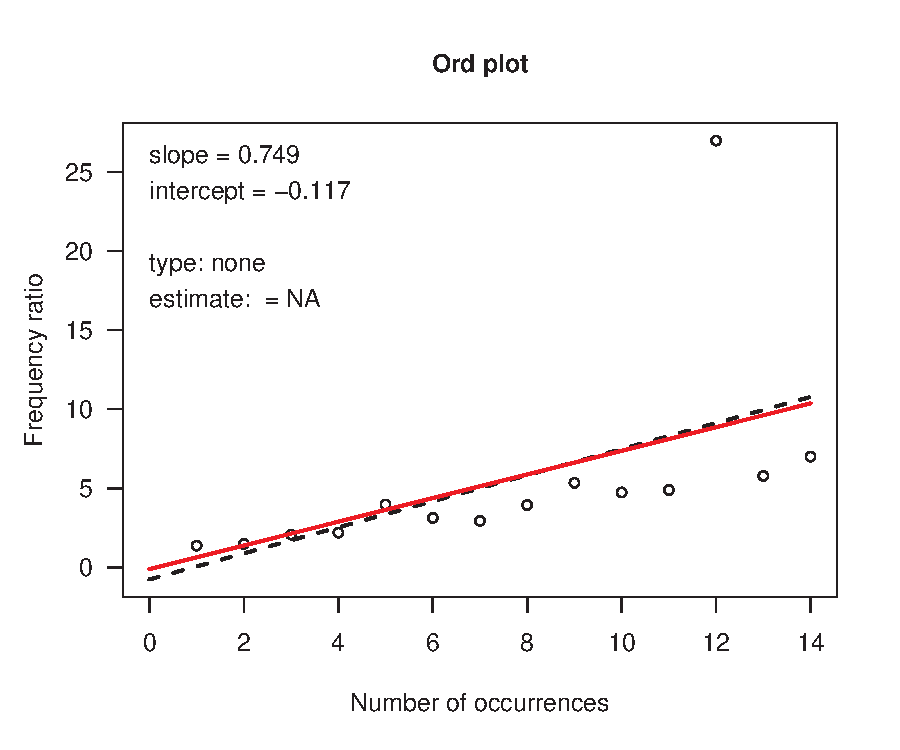
\includegraphics[width=.5\textwidth]{soln/fig/ex3_11b-1} }



\end{knitrout}
      \end{ans}
      
      \item Try to fit a reasonable distribution to describe dependencies among \R packages.
      \begin{ans}
      Among the distributions described in Chapter 3 and implemented in the \pkg{vcd} package
      the negative binomial may be the best to try.
\begin{knitrout}\footnotesize
\definecolor{shadecolor}{rgb}{0.941, 0.941, 0.941}\color{fgcolor}\begin{kframe}
\begin{alltt}
\hlstd{> }\hlstd{dep.gf} \hlkwb{<-} \hlkwd{goodfit}\hlstd{(Depends,} \hlkwc{type}\hlstd{=}\hlstr{"nbinomial"}\hlstd{)}
\hlstd{> }\hlkwd{summary}\hlstd{(dep.gf)}
\end{alltt}
\begin{verbatim}

	 Goodness-of-fit test for nbinomial distribution

                    X^2 df   P(> X^2)
Likelihood Ratio 49.081 12 2.0243e-06
\end{verbatim}
\begin{alltt}
\hlstd{> }\hlkwd{plot}\hlstd{(dep.gf,} \hlkwc{xlab}\hlstd{=}\hlstr{"Number of dependencies"}\hlstd{)}
\hlstd{> }\hlkwd{distplot}\hlstd{(Depends,} \hlkwc{type}\hlstd{=}\hlstr{"nbinomial"}\hlstd{)}
\end{alltt}
\end{kframe}

\centerline{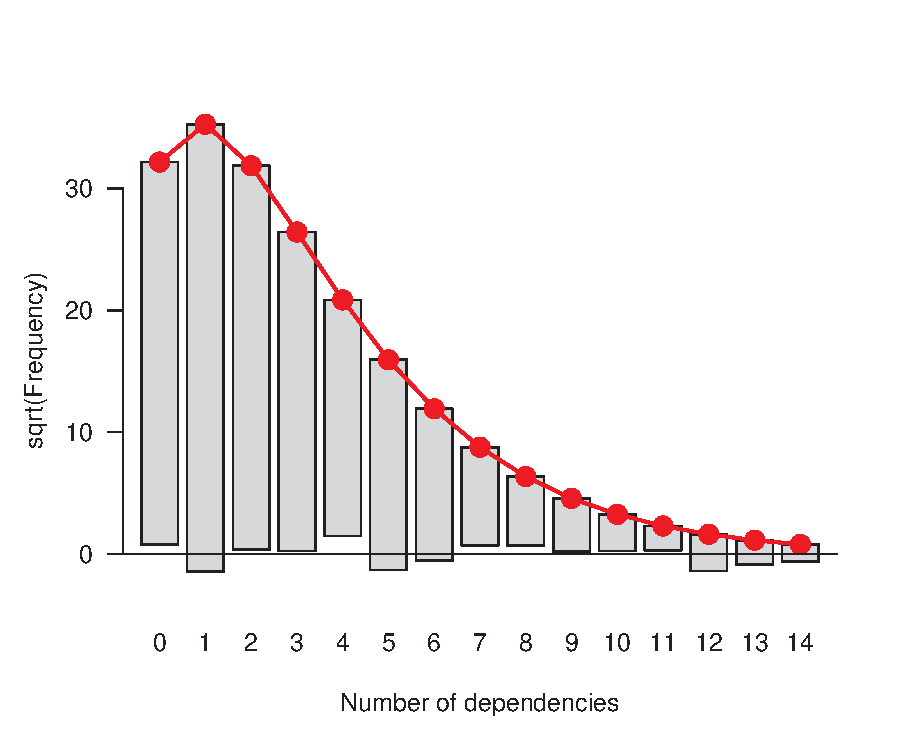
\includegraphics[width=.5\textwidth]{soln/fig/ex3_11c-1} 
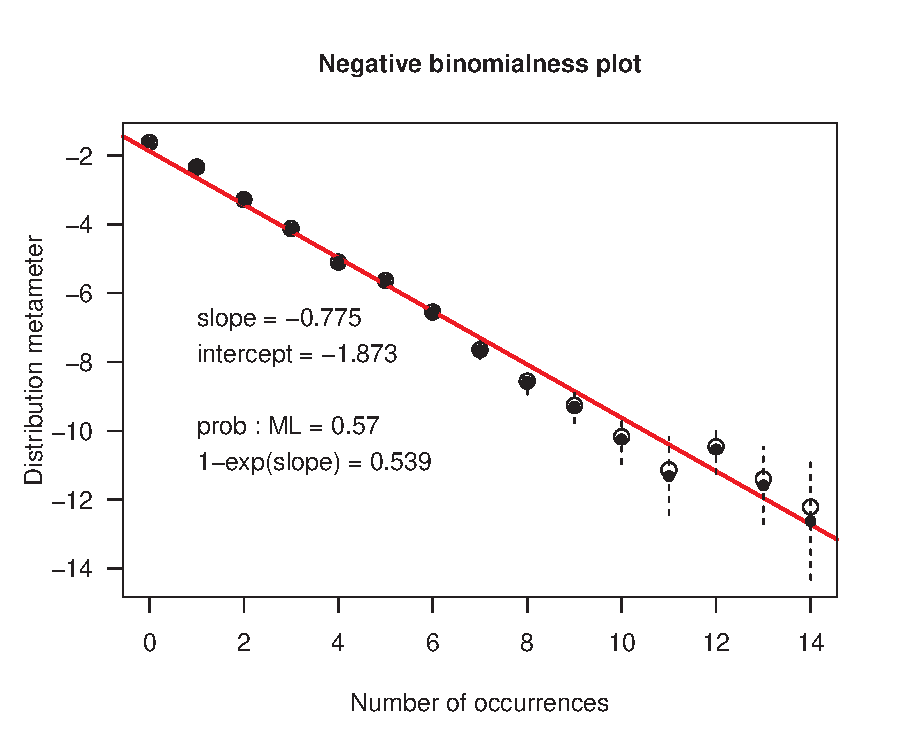
\includegraphics[width=.5\textwidth]{soln/fig/ex3_11c-2} }



\end{knitrout}
      So, this does not fit well, particularly for the packages with many dependencies, but
      it is not altogether terrible.
      The remaining differences come from further heterogeneity for which we haven't got any covariates in the data set. 
      For example, the age of the package would seem like a natural candidate: older packages probably have fewer dependencies.
      \end{ans}
      
    \end{enumerate*}

\exercise\exhard How many years does it take to get into the baseball Hall of Fame?
  The \Rpackage{Lahman} provides a complete record of historical baseball statistics from 1871 to
  the present.  One table, \data{HallOfFame}, records the history of players nominated to
  the Baseball Hall of Fame, and those eventually inducted.  The table below, calculated
  in \help{HallOfFame, package="Lahman"}, records the distribution of the number of years
  taken (from first nomination)
  for the 109 players in the Hall of Fame to be inducted (1936--present).
  Note that \code{years==0} does not, and cannot, occur in this table, so the distribution
  is restricted to positive counts.  Such distributions are called \term{zero-truncated distribution}s.
  Such distributions are like the ordinary ones, but with the probability of zero being zero.
  Thus the other probabilities are scaled up (i.e., divided by $1-\Pr(Y=0)$) so they sum to 1.

% latex table generated in R 3.0.3 by xtable 1.7-3 package
% Sun Sep 14 12:03:39 2014
\begin{tabular}{r|rrrrrrrrrrrrrrr}
  \hline
years    & 1 & 2 & 3 & 4 & 5 & 6 & 7 & 8 & 9 & 10 & 11 & 12 & 13 & 14 & 15 \\
%  \hline
inducted &  46 &  10 &   8 &   7 &   8 &   4 &   2 &   4 &   6 &   3 &   3 &   1 &   4 &   1 &   2 \\
   \hline
\end{tabular}

    \begin{enumerate*}
      \item For the Poisson distribution, show that the zero-truncated probability function can be expressed in the
      form
			\begin{equation*}
			\Pr \{ X = k \given k>0\} =
			  \frac{1}{1-e^{-\lambda}} \times
			  \frac{ e^{ - \lambda } \:  \lambda^k } { k ! }
			  \quad\quad k = 1, 2, \dots
			\end{equation*}
			\begin{ans}
			The standard Poisson distribution has the probability mass function 
			$$
			\Pr \{ X = k \} =  \frac{ e^{ - \lambda } \:  \lambda^k } { k ! } \quad k = 1, 2, \dots \period
			$$
			For this, $\Pr \{ X = 0 \} =  e^{ - \lambda }$. 
			The formula given in the problem
			scales the standard probability to account for zero-truncation, i.e., by the factor
			$\frac{1}{1-\Pr \{ X = 0 \}}$.
			\end{ans}
			

      \item Show that the mean is $\lambda/(1-\exp(-\lambda))$.
      \begin{ans}
      \end{ans}
      
      \item Enter these data into \R as a one-way table, and use \func{goodfit} to fit the standard
      Poisson distribution, as if you hadn't encountered the problem of zero truncation.
      \begin{ans}
      The rootogram below shows why zero truncation needs to be taken into account.
\begin{knitrout}\footnotesize
\definecolor{shadecolor}{rgb}{0.941, 0.941, 0.941}\color{fgcolor}\begin{kframe}
\begin{alltt}
\hlstd{> }\hlstd{years} \hlkwb{<-} \hlnum{1}\hlopt{:}\hlnum{15}
\hlstd{> }\hlstd{inducted} \hlkwb{<-} \hlkwd{c}\hlstd{(}\hlnum{46}\hlstd{,} \hlnum{10}\hlstd{,}  \hlnum{8}\hlstd{,}  \hlnum{7}\hlstd{,}  \hlnum{8}\hlstd{,}  \hlnum{4}\hlstd{,}  \hlnum{2}\hlstd{,}  \hlnum{4}\hlstd{,}  \hlnum{6}\hlstd{,}  \hlnum{3}\hlstd{,}  \hlnum{3}\hlstd{,}  \hlnum{1}\hlstd{,}  \hlnum{4}\hlstd{,}  \hlnum{1}\hlstd{,}  \hlnum{2}\hlstd{)}
\hlstd{> }\hlstd{HOF.df} \hlkwb{<-} \hlkwd{data.frame}\hlstd{(years, inducted)}
\hlstd{> }\hlstd{HOF.tab} \hlkwb{<-} \hlkwd{xtabs}\hlstd{(inducted} \hlopt{~} \hlstd{years,} \hlkwc{data}\hlstd{=HOF.df)}
\hlstd{> }\hlkwd{goodfit}\hlstd{(HOF.tab)}
\end{alltt}
\begin{verbatim}

Observed and fitted values for poisson distribution
with parameters estimated by `ML' 

 count observed     fitted pearson residual
     0        0  1.7081050         -1.30694
     1       46  7.0988218         14.60056
     2       10 14.7512214         -1.23706
     3        8 20.4351783         -2.75082
     4        7 21.2319627         -3.08866
     5        8 17.6478516         -2.29660
     6        4 12.2239706         -2.35221
     7        2  7.2574819         -1.95157
     8        4  3.7702285          0.11833
     9        6  1.7409924          3.22782
    10        3  0.7235500          2.67623
    11        3  0.2733679          5.21498
    12        1  0.0946756          2.94229
    13        4  0.0302668         22.81803
    14        1  0.0089848         10.45503
    15        2  0.0024894         34.54549
\end{verbatim}
\begin{alltt}
\hlstd{> }\hlkwd{summary}\hlstd{(HOF.tab)}
\end{alltt}
\begin{verbatim}
Number of cases in table: 109 
Number of factors: 1 
\end{verbatim}
\begin{alltt}
\hlstd{> }\hlkwd{plot}\hlstd{(}\hlkwd{goodfit}\hlstd{(HOF.tab),} \hlkwc{xlab}\hlstd{=}\hlstr{'Number of years to HOF election'}\hlstd{)}
\end{alltt}
\end{kframe}

\centerline{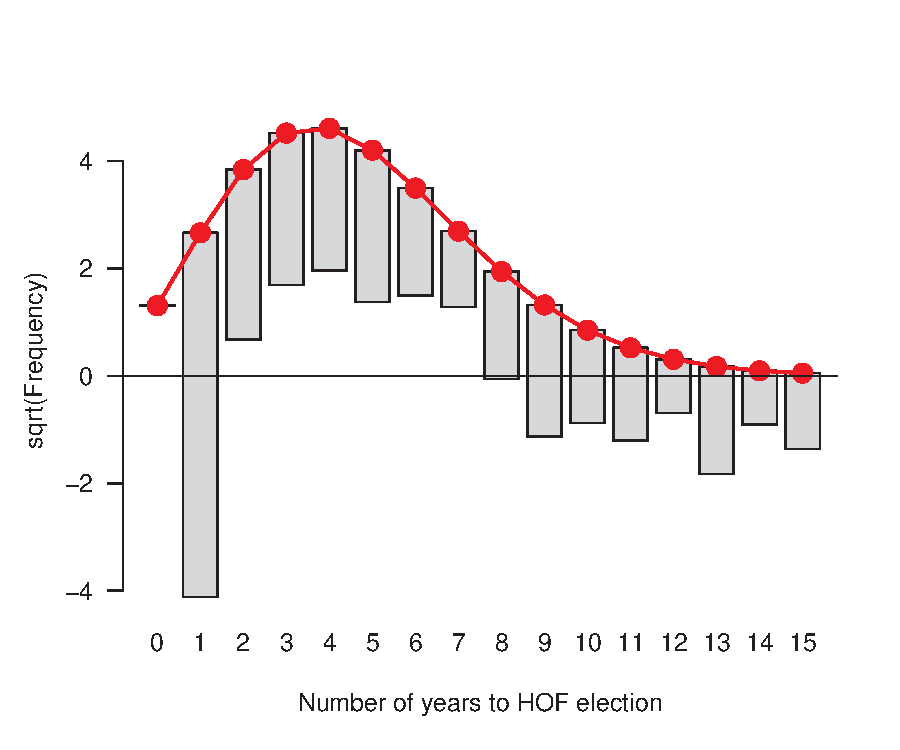
\includegraphics[width=.5\textwidth]{soln/fig/ex3_12c-1} }



\end{knitrout}
      Though not asked in the problem, the zero-truncated Poisson distribution can be fit using \func{vglm}
      in the \Rpackage{VGAM}. %\TODO{One of these is not right.}
\begin{knitrout}\footnotesize
\definecolor{shadecolor}{rgb}{0.941, 0.941, 0.941}\color{fgcolor}\begin{kframe}
\begin{alltt}
\hlstd{> }\hlkwd{library}\hlstd{(VGAM)}
\hlstd{> }\hlstd{hof.tpois0} \hlkwb{<-} \hlkwd{vglm}\hlstd{(years} \hlopt{~} \hlnum{1}\hlstd{,} \hlkwc{family}\hlstd{=pospoisson,} \hlkwc{data}\hlstd{=HOF.df,} \hlkwc{weights}\hlstd{=inducted)}
\hlstd{> }\hlstd{hof.tpois0}
\end{alltt}
\begin{verbatim}
Call:
vglm(formula = years ~ 1, family = pospoisson, data = HOF.df, 
    weights = inducted)

Coefficients:
(Intercept) 
     1.4076 

Degrees of Freedom: 15 Total; 14 Residual
Log-likelihood: -339.31 
\end{verbatim}
\end{kframe}
\end{knitrout}
      Models for count data, taking account of excess zeros or zero truncation are examined in more detail
      in Chapter 11.  There, we use the \Rpackage{countreg}, that provides a \func{zerotrunc} function for these
      problems.  The zero truncated negative binomial provides a better fit than the zero truncated Poisson,
      but that is not great either.
\begin{knitrout}\footnotesize
\definecolor{shadecolor}{rgb}{0.941, 0.941, 0.941}\color{fgcolor}\begin{kframe}
\begin{alltt}
\hlstd{> }\hlkwd{library}\hlstd{(countreg)}
\hlstd{> }\hlstd{hof.zerot0} \hlkwb{<-} \hlkwd{zerotrunc}\hlstd{(years} \hlopt{~} \hlnum{1}\hlstd{,} \hlkwc{weights} \hlstd{= inducted,} \hlkwc{data}\hlstd{=HOF.df)}
\hlstd{> }\hlstd{hof.zerot1} \hlkwb{<-} \hlkwd{zerotrunc}\hlstd{(years} \hlopt{~} \hlnum{1}\hlstd{,} \hlkwc{weights} \hlstd{= inducted,} \hlkwc{dist}\hlstd{=}\hlstr{"negbin"}\hlstd{)}
\hlstd{> }\hlstd{countreg}\hlopt{::}\hlkwd{rootogram}\hlstd{(hof.zerot0)}
\hlstd{> }\hlstd{countreg}\hlopt{::}\hlkwd{rootogram}\hlstd{(hof.zerot1)}
\end{alltt}
\end{kframe}

\centerline{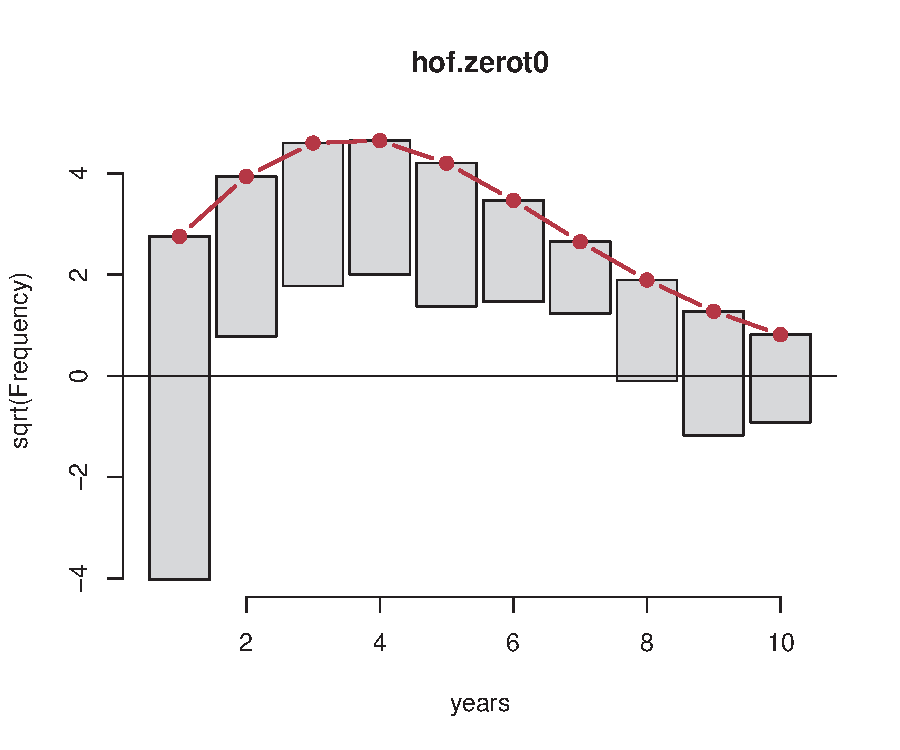
\includegraphics[width=.5\textwidth]{soln/fig/ex3_12d-1} 
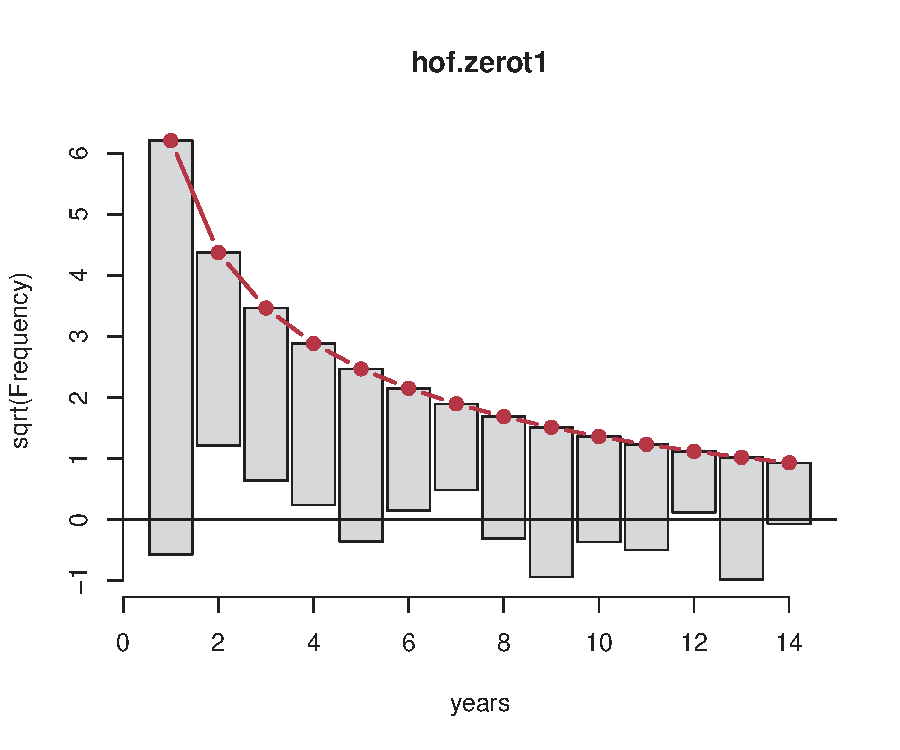
\includegraphics[width=.5\textwidth]{soln/fig/ex3_12d-2} }



\end{knitrout}

      \end{ans}
      

    \end{enumerate*}


\end{Exercises}


\clearpage
\chapter{Two-Way Contingency Tables}\label{ch:twoway}

%\section{Lab exercises}\label{sec:twoway-lab}

\begin{Exercises}

  \exercise The data set \code{fat}, created below, gives a $2 \times 2$ table recording the level of
  cholesterol in diet and the presence of symptoms of heart disease for a sample of
  23 people.

\begin{knitrout}\footnotesize
\definecolor{shadecolor}{rgb}{0.941, 0.941, 0.941}\color{fgcolor}\begin{kframe}
\begin{alltt}
\hlstd{> }\hlstd{fat} \hlkwb{<-} \hlkwd{matrix}\hlstd{(}\hlkwd{c}\hlstd{(}\hlnum{6}\hlstd{,} \hlnum{4}\hlstd{,} \hlnum{2}\hlstd{,} \hlnum{11}\hlstd{),} \hlnum{2}\hlstd{,} \hlnum{2}\hlstd{)}
\hlstd{> }\hlkwd{dimnames}\hlstd{(fat)} \hlkwb{<-} \hlkwd{list}\hlstd{(}\hlkwc{diet} \hlstd{=} \hlkwd{c}\hlstd{(}\hlstr{"LoChol"}\hlstd{,} \hlstr{"HiChol"}\hlstd{),}
\hlstd{+ }                      \hlkwc{disease} \hlstd{=} \hlkwd{c}\hlstd{(}\hlstr{"No"}\hlstd{,} \hlstr{"Yes"}\hlstd{))}
\end{alltt}
\end{kframe}
\end{knitrout}

  \begin{enumerate*}
    \item Use \code{chisq.test(fat)} to test for association between diet and disease.
    Is there any indication that this test may not be appropriate here?
    \begin{ans}
    \end{ans}
    
    
    \item Use a fourfold display to test this association visually.  Experiment with    
    the different options for standardizing the margins, using the \code{margin}
    argument to \func{fourfold}. What evidence is shown in different displays regarding
    whether the odds ratio differs significantly from 1?
    \begin{ans}
    \end{ans}
    
    \item \code{oddsratio(fat, log = FALSE)} will give you a numerical answer.  How does
    this compare to your visual impression from fourfold displays?
    \begin{ans}
    \end{ans}
    
    \item With such a small sample, Fisher's exact test may be more reliable for statistical
    inference.  Use \code{fisher.test(fat)}, and compare these results to what you have
    observed before.
    \begin{ans}
    \end{ans}
    
    \item Write a one-paragraph summary of your findings and conclusions for this data set.
    \begin{ans}
    \end{ans}
    
  \end{enumerate*}

  \exercise The data set \data{Abortion} in \pkg{vcdExtra} gives a $2 \times 2 \times 2$
  table of opinions regarding abortion in relation to sex and status of the
  respondent. This table has the following structure:
\begin{knitrout}\footnotesize
\definecolor{shadecolor}{rgb}{0.941, 0.941, 0.941}\color{fgcolor}\begin{kframe}
\begin{alltt}
\hlstd{> }\hlkwd{data}\hlstd{(}\hlstr{"Abortion"}\hlstd{,} \hlkwc{package} \hlstd{=} \hlstr{"vcdExtra"}\hlstd{)}
\hlstd{> }\hlkwd{str}\hlstd{(Abortion)}
\end{alltt}
\begin{verbatim}
 table [1:2, 1:2, 1:2] 171 152 138 167 79 148 112 133
 - attr(*, "dimnames")=List of 3
  ..$ Sex             : chr [1:2] "Female" "Male"
  ..$ Status          : chr [1:2] "Lo" "Hi"
  ..$ Support_Abortion: chr [1:2] "Yes" "No"
\end{verbatim}
\end{kframe}
\end{knitrout}
  \begin{enumerate*}
    \item Taking support for abortion as the outcome variable, produce fourfold displays   
    showing the association with sex, stratified by status.
    \begin{ans}
\begin{knitrout}\footnotesize
\definecolor{shadecolor}{rgb}{0.941, 0.941, 0.941}\color{fgcolor}\begin{kframe}
\begin{alltt}
\hlstd{> }\hlkwd{data}\hlstd{(}\hlstr{"Abortion"}\hlstd{,} \hlkwc{package}\hlstd{=}\hlstr{"vcdExtra"}\hlstd{)}
\hlstd{> }\hlkwd{structable}\hlstd{(Abortion)}
\end{alltt}
\begin{verbatim}
                        Status  Lo  Hi
Sex    Support_Abortion               
Female Yes                     171 138
       No                       79 112
Male   Yes                     152 167
       No                      148 133
\end{verbatim}
\begin{alltt}
\hlstd{> }\hlstd{Abortion2}\hlkwb{<-}\hlkwd{aperm}\hlstd{(Abortion,} \hlkwd{c}\hlstd{(}\hlnum{1}\hlstd{,}\hlnum{3}\hlstd{,}\hlnum{2}\hlstd{))}
\hlstd{> }\hlkwd{fourfold}\hlstd{(Abortion2)}
\end{alltt}
\end{kframe}

\centerline{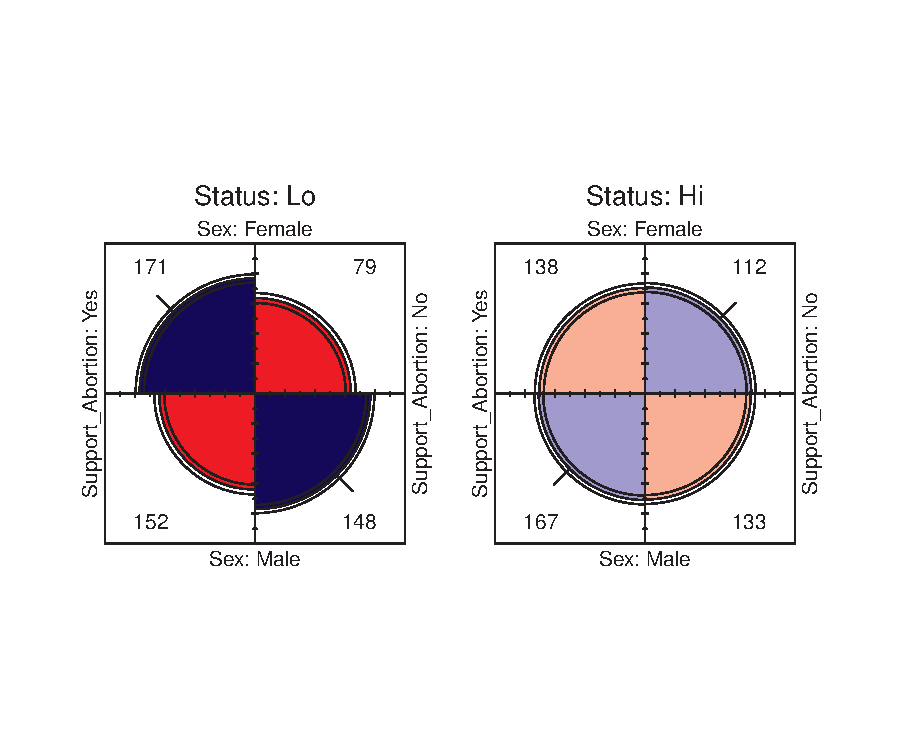
\includegraphics[width=.5\textwidth]{soln/fig/ex4_2a-1} }



\end{knitrout}
    \end{ans}
    
    \item Do the same for the association of support for abortion with status, stratified
    by sex.
    \begin{ans}
\begin{knitrout}\footnotesize
\definecolor{shadecolor}{rgb}{0.941, 0.941, 0.941}\color{fgcolor}\begin{kframe}
\begin{alltt}
\hlstd{> }\hlstd{Abortion3}\hlkwb{<-}\hlkwd{aperm}\hlstd{(Abortion,} \hlkwd{c}\hlstd{(}\hlnum{2}\hlstd{,}\hlnum{3}\hlstd{,}\hlnum{1}\hlstd{))}
\hlstd{> }\hlkwd{fourfold}\hlstd{(Abortion3)}
\end{alltt}
\end{kframe}

\centerline{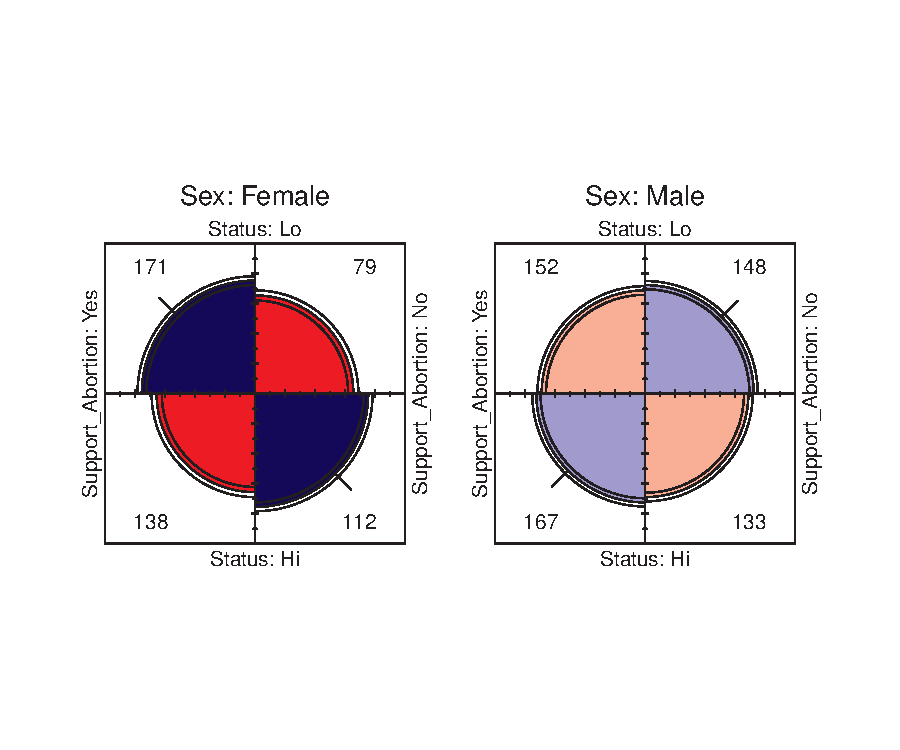
\includegraphics[width=.5\textwidth]{soln/fig/ex4_2b-1} }



\end{knitrout}
    \end{ans}
    
    \item For each of the problems above, use \func{oddsratio} to calculate the numerical
    values of the odds ratio, as stratified in the question.
    \begin{ans}
\begin{knitrout}\footnotesize
\definecolor{shadecolor}{rgb}{0.941, 0.941, 0.941}\color{fgcolor}\begin{kframe}
\begin{alltt}
\hlstd{> }     \hlcom{# Sex by support for abortion, stratified by status}
\hlstd{> }\hlkwd{summary}\hlstd{(}\hlkwd{oddsratio}\hlstd{(Abortion2))}
\end{alltt}
\begin{verbatim}

z test of coefficients:

                      Estimate Std. Error z value Pr(>|z|)    
Female:Male/Yes:No|Lo   0.7455     0.1784    4.18  2.9e-05 ***
Female:Male/Yes:No|Hi  -0.0189     0.1723   -0.11     0.91    
---
Signif. codes:  0 '***' 0.001 '**' 0.01 '*' 0.05 '.' 0.1 ' ' 1
\end{verbatim}
\begin{alltt}
\hlstd{> }     \hlcom{# Status by support for abortion, stratified by sex}
\hlstd{> }\hlkwd{summary}\hlstd{(}\hlkwd{oddsratio}\hlstd{(Abortion3))}
\end{alltt}
\begin{verbatim}

z test of coefficients:

                    Estimate Std. Error z value Pr(>|z|)   
Lo:Hi/Yes:No|Female    0.563      0.186    3.03   0.0025 **
Lo:Hi/Yes:No|Male     -0.201      0.164   -1.23   0.2199   
---
Signif. codes:  0 '***' 0.001 '**' 0.01 '*' 0.05 '.' 0.1 ' ' 1
\end{verbatim}
\end{kframe}
\end{knitrout}
    \end{ans}
    
    \item Write a brief summary of how support for abortion depends on sex and status.
    \begin{ans}
    Regardless of status, more women say no to abortion and more men say yes. 
    Regardless of gender, more low status say no and more high status say yes.
    \end{ans}
    
  \end{enumerate*}

  \exercise The \data{JobSat} table on income and job satisfaction
  created in \exref{ex:jobsat1} is contained in the
  \Rpackage{vcdExtra}.
  \begin{enumerate*}
    \item Carry out a standard $\chi^2$ test for association between income and job satisfaction.
    Is there any indication that this test might not be appropriate?
      Repeat this test using \code{simulate.p.value = TRUE} to obtain a Monte Carlo
      test that does not depend on large sample size.  Does this change your
      conclusion?
    \begin{ans}
    \end{ans}
    
    \item Both variables are ordinal, so CMH tests may be more powerful here.
    Carry out that analysis.  What do you conclude?
    \begin{ans}
    \end{ans}
    
  \end{enumerate*}

  \exercise The \data{Hospital} data in \pkg{vcd} gives a $3 \times 3$ table
  relating the length of stay (in years) of 132 long-term schizophrenic patients in two London mental hospitals with the frequency of visits
  by family and friends.
    \begin{enumerate*}
      \item Carry out a  $\chi^2$ test for association between the two
      variables.
      \begin{ans}
\begin{knitrout}\footnotesize
\definecolor{shadecolor}{rgb}{0.941, 0.941, 0.941}\color{fgcolor}\begin{kframe}
\begin{alltt}
\hlstd{> }\hlkwd{data}\hlstd{(}\hlstr{"Hospital"}\hlstd{,} \hlkwc{package}\hlstd{=}\hlstr{"vcd"}\hlstd{)}
\hlstd{> }\hlkwd{chisq.test}\hlstd{(Hospital)}
\end{alltt}
\begin{verbatim}

	Pearson's Chi-squared test

data:  Hospital
X-squared = 35.2, df = 4, p-value = 4.3e-07
\end{verbatim}
\end{kframe}
\end{knitrout}
      \end{ans}
      
      \item Use \func{assocstats} to compute association statistics.
      How would you describe the strength of association here?
      \begin{ans}
\begin{knitrout}\footnotesize
\definecolor{shadecolor}{rgb}{0.941, 0.941, 0.941}\color{fgcolor}\begin{kframe}
\begin{alltt}
\hlstd{> }\hlkwd{assocstats}\hlstd{(Hospital)}
\end{alltt}
\begin{verbatim}
                    X^2 df   P(> X^2)
Likelihood Ratio 38.353  4 9.4755e-08
Pearson          35.171  4 4.2842e-07

Phi-Coefficient   : NA 
Contingency Coeff.: 0.459 
Cramer's V        : 0.365 
\end{verbatim}
\end{kframe}
\end{knitrout}
      By the contingency coefficient, there is moderately strong association between the length
      of stay long-term schizophrenic patients and the frequency of visits by family and friends.
      \end{ans}
      
      \item Produce an association plot for these data, with
      visit frequency as the vertical variable.  Describe the
      pattern of the relation you see here.
      \begin{ans}
\begin{knitrout}\footnotesize
\definecolor{shadecolor}{rgb}{0.941, 0.941, 0.941}\color{fgcolor}\begin{kframe}
\begin{alltt}
\hlstd{> }\hlkwd{assoc}\hlstd{(Hospital,} \hlkwc{shade}\hlstd{=}\hlnum{TRUE}\hlstd{)}
\end{alltt}
\end{kframe}

\centerline{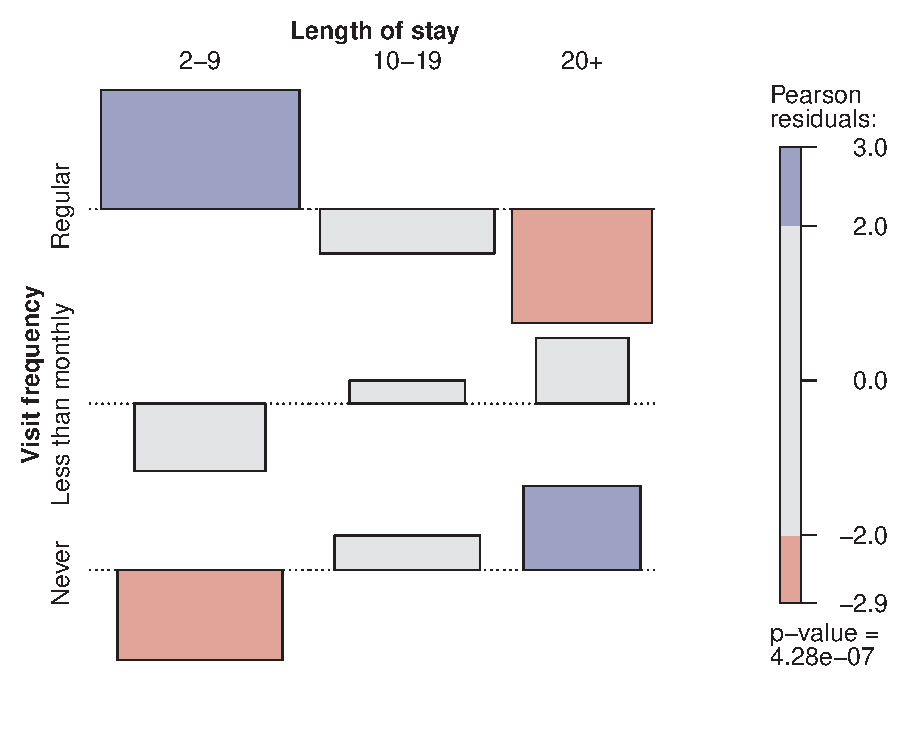
\includegraphics[width=.5\textwidth]{soln/fig/ex4_4c-1} }



\end{knitrout}
      \end{ans}
      
      \item Both variables can be considered ordinal, so
      \func{CMHtest} may be useful here.  Carry out that
      analysis.  Do any of the tests lead to different conclusions?
      \begin{ans}
\begin{knitrout}\footnotesize
\definecolor{shadecolor}{rgb}{0.941, 0.941, 0.941}\color{fgcolor}\begin{kframe}
\begin{alltt}
\hlstd{> }\hlkwd{CMHtest}\hlstd{(Hospital)}
\end{alltt}
\begin{verbatim}
Cochran-Mantel-Haenszel Statistics for Visit frequency by Length of stay 

                 AltHypothesis Chisq Df     Prob
cor        Nonzero correlation  29.1  1 6.74e-08
rmeans  Row mean scores differ  34.4  2 3.40e-08
cmeans  Col mean scores differ  29.6  2 3.72e-07
general    General association  34.9  4 4.86e-07
\end{verbatim}
\end{kframe}
\end{knitrout}
      The results of all four tests lead to the same conclusion that there is a
      significant association between the visit frequency and the length of stay.
      The test for non-zero correlation, trteating both variables as ordinal, has the
      largest ratio of $\chi^2 /df$.
      \end{ans}
      
    \end{enumerate*}

  \exercise Continuing with the \data{Hospital} data:
    \begin{enumerate*}
      \item Try one or more of the following other functions for visualizing two-way contingency tables with this data: 
      \func{plot}, \func{tile}, \func{mosaic}, and \func{spineplot}.  
      [For all except \func{spineplot}, it is useful to include the argument \code{shade=TRUE}].
      \begin{ans}
\begin{knitrout}\footnotesize
\definecolor{shadecolor}{rgb}{0.941, 0.941, 0.941}\color{fgcolor}\begin{kframe}
\begin{alltt}
\hlstd{> }\hlkwd{plot}\hlstd{(Hospital,} \hlkwc{shade}\hlstd{=}\hlnum{TRUE}\hlstd{)}
\hlstd{> }\hlkwd{tile}\hlstd{(Hospital,} \hlkwc{shade}\hlstd{=}\hlnum{TRUE}\hlstd{)}
\end{alltt}
\end{kframe}

\centerline{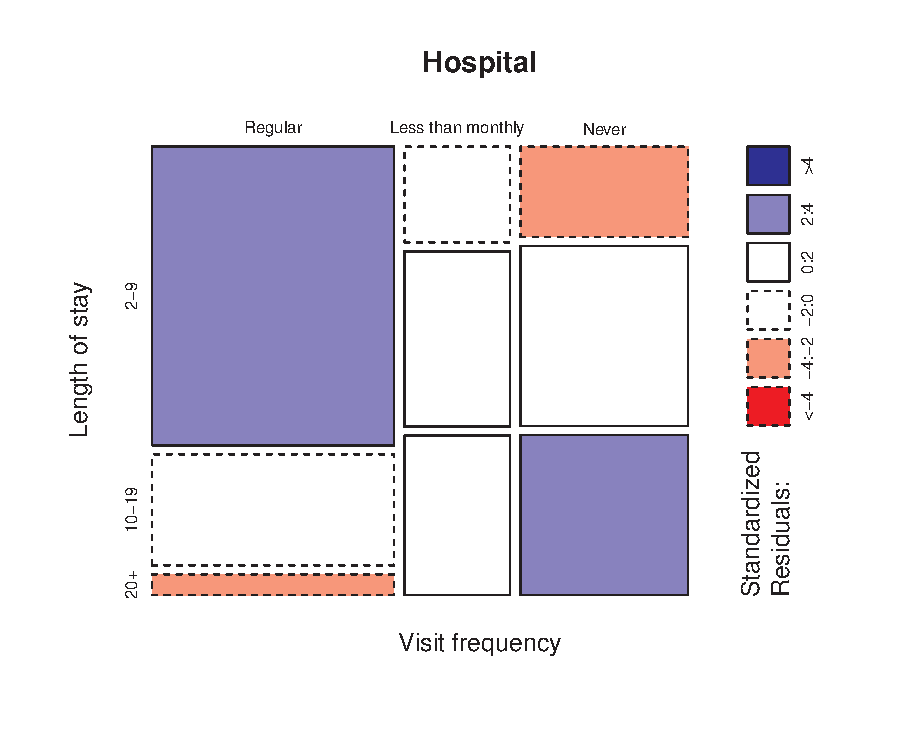
\includegraphics[width=.5\textwidth]{soln/fig/ex4_5a1-1} 
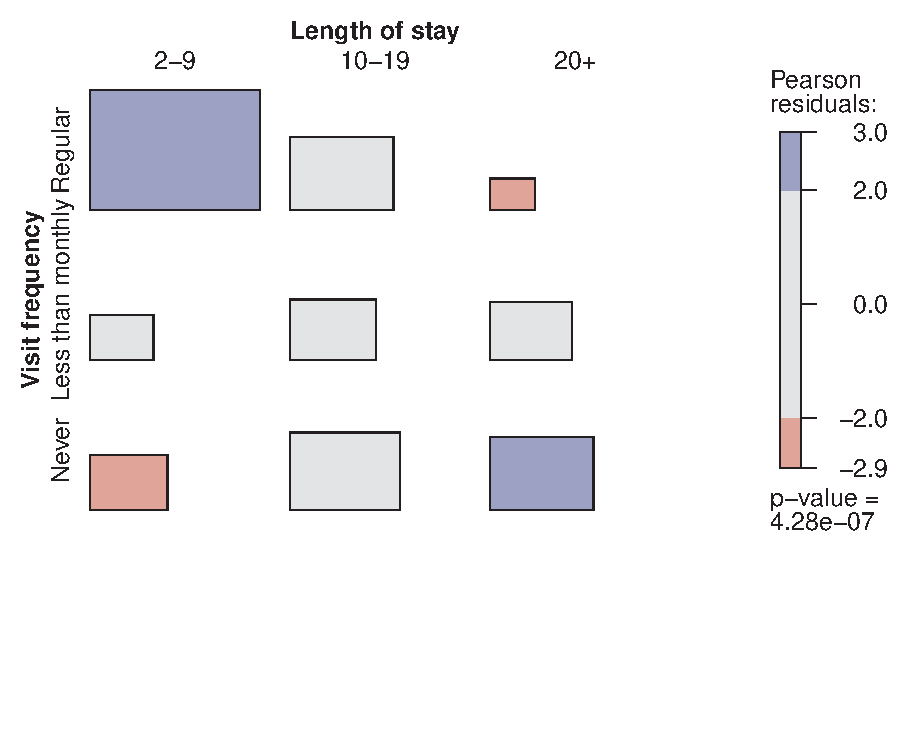
\includegraphics[width=.5\textwidth]{soln/fig/ex4_5a1-2} }



\end{knitrout}
      \end{ans}
      \begin{ans}
\begin{knitrout}\footnotesize
\definecolor{shadecolor}{rgb}{0.941, 0.941, 0.941}\color{fgcolor}\begin{kframe}
\begin{alltt}
\hlstd{> }\hlkwd{mosaic}\hlstd{(Hospital,} \hlkwc{shade}\hlstd{=}\hlnum{TRUE}\hlstd{)}
\hlstd{> }\hlkwd{spineplot}\hlstd{(Hospital)}
\end{alltt}
\end{kframe}

\centerline{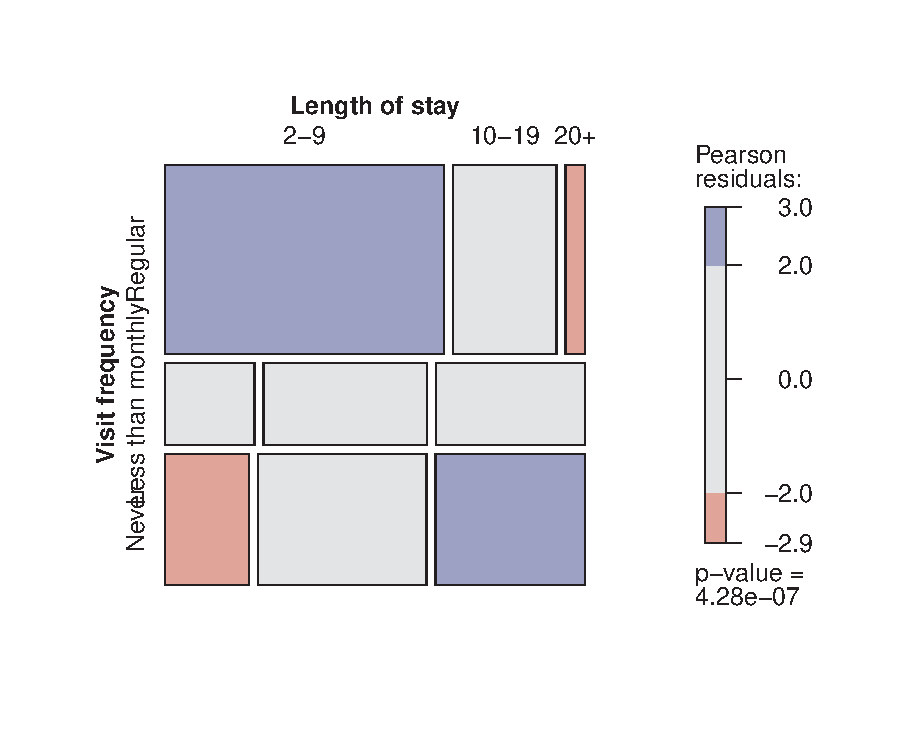
\includegraphics[width=.5\textwidth]{soln/fig/ex4_5a2-1} 
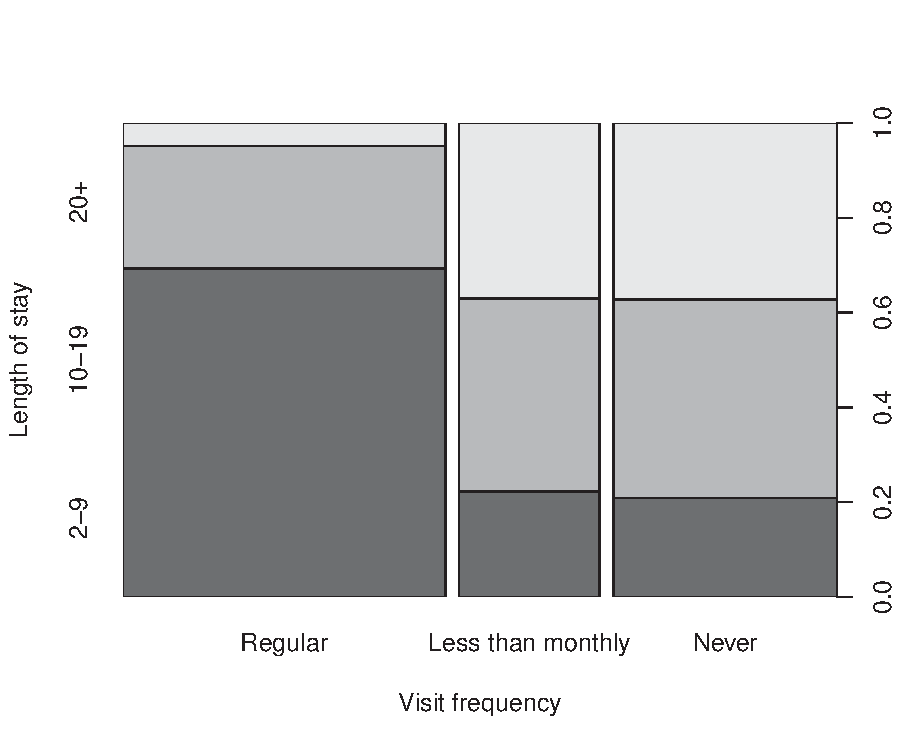
\includegraphics[width=.5\textwidth]{soln/fig/ex4_5a2-2} }



\end{knitrout}
      \end{ans}
      
      \item Comment on the differences among these displays for understanding the relation between 
      visits and length of stay.
      \begin{ans}
      \end{ans}
      
    \end{enumerate*}
  
  \exercise The two-way table \data{Mammograms} in \pkg{vcdExtra} gives ratings
  on the severity of diagnosis of 110 mammograms by two raters.
    \begin{enumerate*}
      \item Assess the strength of agreement between the raters using Cohen's
      $\kappa$, both unweighted and weighted.
      \begin{ans}
      Both unweighted and weighted $\kappa$ indicate substantial agreement.
      Fleiss-Cohen weights give greater weight to the ``near-misses,'' so gives
      a larger value.
\begin{knitrout}\footnotesize
\definecolor{shadecolor}{rgb}{0.941, 0.941, 0.941}\color{fgcolor}\begin{kframe}
\begin{alltt}
\hlstd{> }\hlkwd{Kappa}\hlstd{(Mammograms)}
\end{alltt}
\begin{verbatim}
           value    ASE     z Pr(>|z|)
Unweighted 0.371 0.0603  6.15 7.56e-10
Weighted   0.596 0.0492 12.11 8.90e-34
\end{verbatim}
\begin{alltt}
\hlstd{> }\hlkwd{Kappa}\hlstd{(Mammograms,} \hlkwc{weights}\hlstd{=} \hlstr{"Fleiss-Cohen"}\hlstd{)}
\end{alltt}
\begin{verbatim}
           value    ASE     z Pr(>|z|)
Unweighted 0.371 0.0603  6.15 7.56e-10
Weighted   0.764 0.0400 19.12 1.67e-81
\end{verbatim}
\end{kframe}
\end{knitrout}

      \end{ans}
      
      \item Use \func{agreementplot} for a graphical display of agreement here.
      \begin{ans}
      The default for \func{agreementplot} shows the weighted display, so you can use \code{weights=1}
      for the unweighted version.
\begin{knitrout}\footnotesize
\definecolor{shadecolor}{rgb}{0.941, 0.941, 0.941}\color{fgcolor}\begin{kframe}
\begin{alltt}
\hlstd{> }\hlkwd{agreementplot}\hlstd{(Mammograms,} \hlkwc{main}\hlstd{=}\hlstr{"Unweighted"}\hlstd{,} \hlkwc{weights}\hlstd{=}\hlnum{1}\hlstd{)}
\hlstd{> }\hlkwd{agreementplot}\hlstd{(Mammograms,} \hlkwc{main}\hlstd{=}\hlstr{"Weighted"}\hlstd{)}
\end{alltt}
\end{kframe}

\centerline{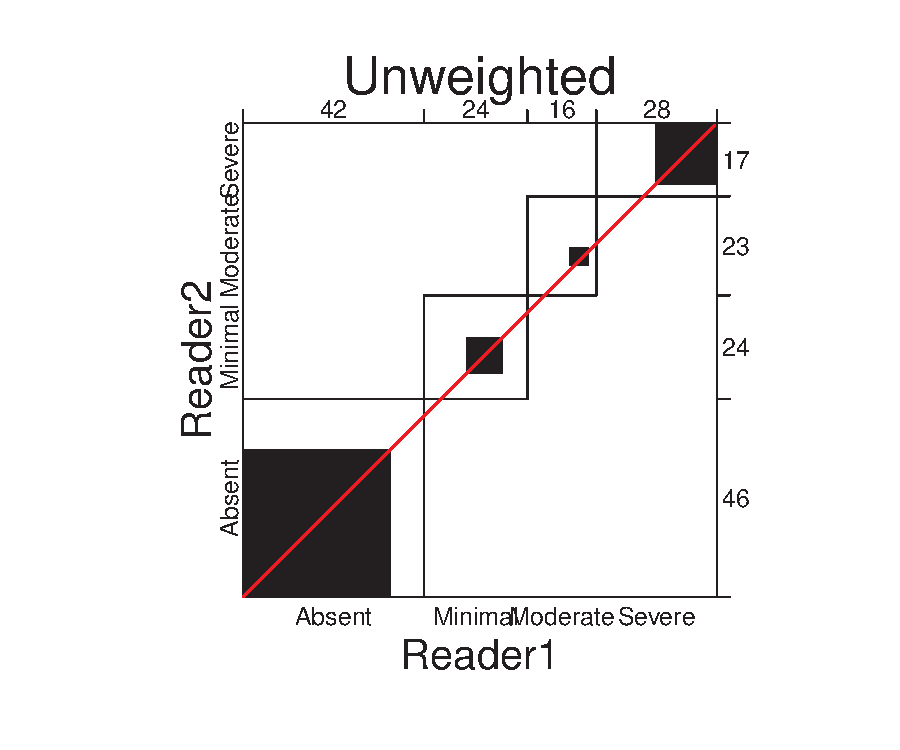
\includegraphics[width=.5\textwidth]{soln/fig/ex4_6b-1} 
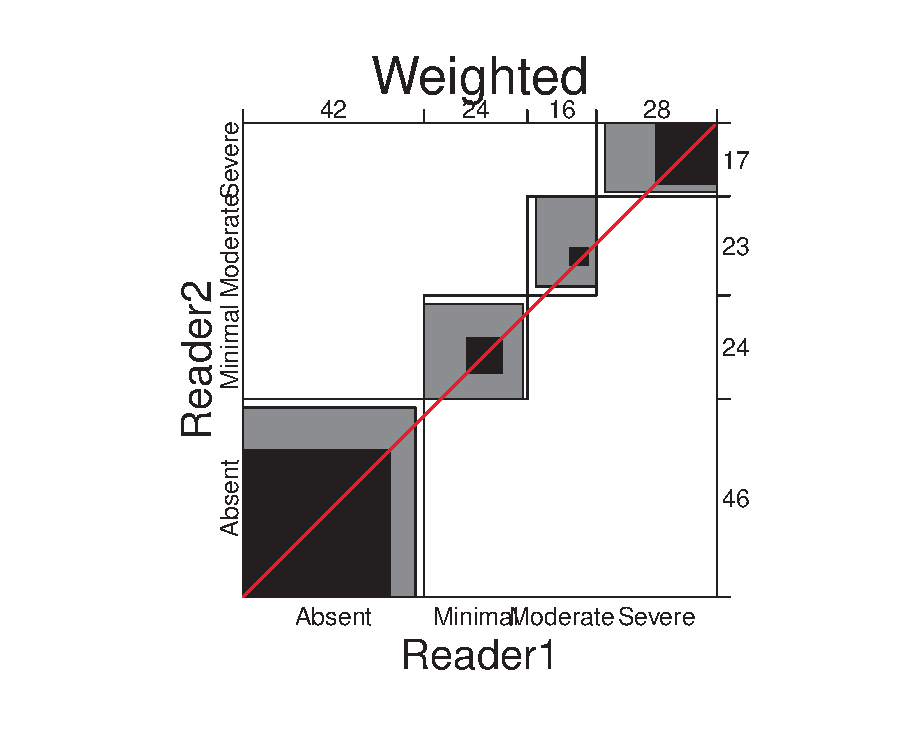
\includegraphics[width=.5\textwidth]{soln/fig/ex4_6b-2} }



\end{knitrout}
      \end{ans}
      
      \item Compare the Kappa measures with the results from \func{assocstats}. 
      What is a reasonable interpretation of each of these measures?
      \begin{ans}
      The contingency coefficient and Cramer's V assess only association, so these could be large when
      there is little agreement. The values of these statistics are not directly comparable. 
\begin{knitrout}\footnotesize
\definecolor{shadecolor}{rgb}{0.941, 0.941, 0.941}\color{fgcolor}\begin{kframe}
\begin{alltt}
\hlstd{> }\hlkwd{assocstats}\hlstd{(Mammograms)}
\end{alltt}
\begin{verbatim}
                    X^2 df   P(> X^2)
Likelihood Ratio 92.619  9 4.4409e-16
Pearson          83.516  9 3.2307e-14

Phi-Coefficient   : NA 
Contingency Coeff.: 0.657 
Cramer's V        : 0.503 
\end{verbatim}
\end{kframe}
\end{knitrout}
      \end{ans}
      
    \end{enumerate*}

  \exercise \citet{AgrestiWinner:1997} gave the data in \tabref{tab:siskel-ebert} on the
  ratings of 160 movies by the reviewers Gene Siskel and Roger Ebert for the period
  from April 1995 through September 1996. The rating categories were Con (``thumbs down''),
  Mixed, and Pro (``thumbs up'').
  \begin{table}[!htb]
\centering
\caption{Movie ratings by Siskel \& Ebert, April 1995--September 1996. \emph{Source}: \citet{AgrestiWinner:1997}}\label{tab:siskel-ebert}
\begin{tabular}{rr|lll|l}
        &       &  \multicolumn{3}{|c|}{Ebert} \\
        &       & Con & Mixed & Pro & Total \\ \hline
        & Con   &  24 &   8   &  13 &  45   \\
 Siskel & Mixed &   8 &  13   &  11 &  32   \\
        & Pro   &  10 &   9   &  64 &  83   \\ \hline
        & Total &  42 &  30   &  88 & 160   \\
\end{tabular}
\end{table}
  \begin{enumerate*}
     \item Assess the strength of agreement between the raters using Cohen's
       $\kappa$, both unweighted and weighted.
       \begin{ans}
\begin{knitrout}\footnotesize
\definecolor{shadecolor}{rgb}{0.941, 0.941, 0.941}\color{fgcolor}\begin{kframe}
\begin{alltt}
\hlstd{> }\hlstd{ratings} \hlkwb{<-} \hlkwd{matrix}\hlstd{(}
\hlstd{+ }\hlkwd{c}\hlstd{(}
\hlstd{+ }  \hlnum{24}\hlstd{,}  \hlnum{8}\hlstd{,} \hlnum{13}\hlstd{,}
\hlstd{+ }   \hlnum{8}\hlstd{,} \hlnum{13}\hlstd{,} \hlnum{11}\hlstd{,}
\hlstd{+ }  \hlnum{10}\hlstd{,}  \hlnum{9}\hlstd{,} \hlnum{64}
\hlstd{+ } \hlstd{),} \hlnum{3}\hlstd{,} \hlnum{3}\hlstd{,} \hlkwc{byrow}\hlstd{=}\hlnum{TRUE}\hlstd{)}
\hlstd{> }\hlkwd{dimnames}\hlstd{(ratings)} \hlkwb{<-} \hlkwd{list}\hlstd{(}\hlkwc{Siskal}\hlstd{=}\hlkwd{c}\hlstd{(}\hlstr{"Con"}\hlstd{,} \hlstr{"Mixed"}\hlstd{,} \hlstr{"Pro"}\hlstd{),}
\hlstd{+ }                          \hlkwc{Ebert} \hlstd{=}\hlkwd{c}\hlstd{(}\hlstr{"Con"}\hlstd{,} \hlstr{"Mixed"}\hlstd{,} \hlstr{"Pro"}\hlstd{))}
\hlstd{> }\hlkwd{Kappa}\hlstd{(ratings)}
\end{alltt}
\begin{verbatim}
           value    ASE    z Pr(>|z|)
Unweighted 0.389 0.0598 6.50 7.87e-11
Weighted   0.427 0.0635 6.72 1.78e-11
\end{verbatim}
\end{kframe}
\end{knitrout}
       \end{ans}
       
     \item Use \func{agreementplot} for a graphical display of agreement here.
     \begin{ans}
     The agreement plot shows that both Siskal and Ebert most commonly gave
     ``thumbs up'' ratings where they largely agreed.  Their ratings differed
     most when one of them gave a Mixed rating.
\begin{knitrout}\footnotesize
\definecolor{shadecolor}{rgb}{0.941, 0.941, 0.941}\color{fgcolor}\begin{kframe}
\begin{alltt}
\hlstd{> }\hlkwd{agreementplot}\hlstd{(ratings)}
\end{alltt}
\end{kframe}

\centerline{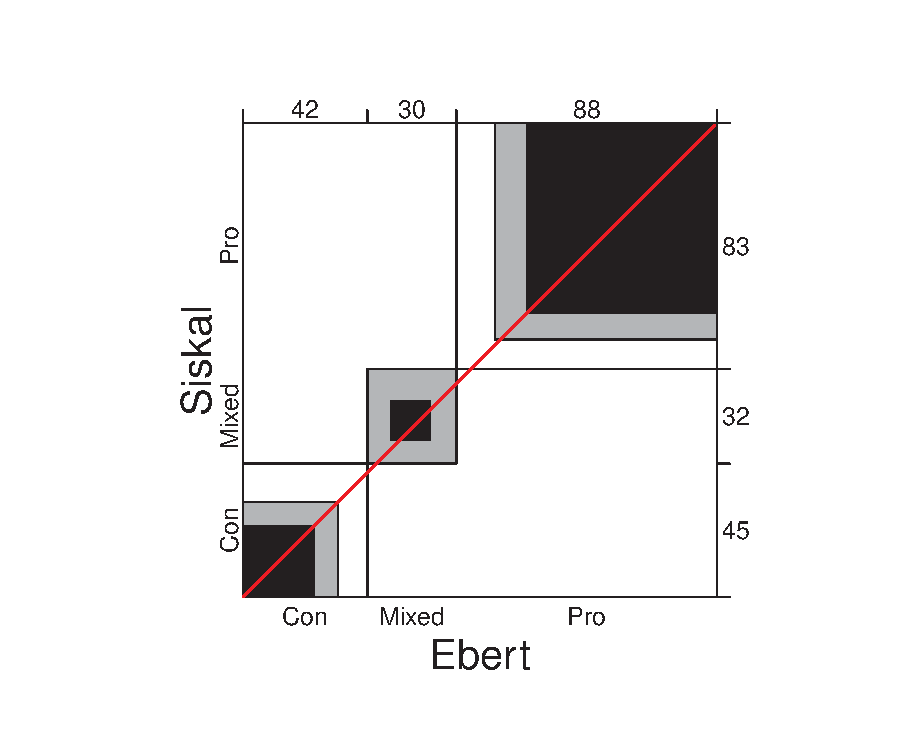
\includegraphics[width=.5\textwidth]{soln/fig/ex4_8b-1} }



\end{knitrout}
     \end{ans}
     
     \item Assess the hypothesis that the ratings are \emph{symmetric} around the
       main diagonal, using an appropriate $\chi^2$ test.
       \emph{Hint}:  Symmetry for a square table $\mat{T}$ means that $t_{ij} = t_{ji}$
       for $i \ne j$.  The expected frequencies under the hypothesis of symmetry
       are the average of the off-diagonal cells,
       $\mat{E} = (\mat{T} + \mat{T}\trans) / 2$.
     \begin{ans}
\begin{knitrout}\footnotesize
\definecolor{shadecolor}{rgb}{0.941, 0.941, 0.941}\color{fgcolor}\begin{kframe}
\begin{alltt}
\hlstd{> }\hlstd{T} \hlkwb{<-} \hlstd{(ratings} \hlopt{+} \hlkwd{t}\hlstd{(ratings))}\hlopt{/}\hlnum{2}
\hlstd{> }\hlstd{(Chisq} \hlkwb{<-} \hlkwd{sum}\hlstd{((ratings} \hlopt{-} \hlstd{T)}\hlopt{^}\hlnum{2} \hlopt{/} \hlstd{T))}
\end{alltt}
\begin{verbatim}
[1] 0.5913
\end{verbatim}
\begin{alltt}
\hlstd{> }\hlstd{df} \hlkwb{<-} \hlkwd{nrow}\hlstd{(T)} \hlopt{*} \hlstd{(}\hlkwd{nrow}\hlstd{(T)}\hlopt{-}\hlnum{1}\hlstd{)} \hlopt{/}\hlnum{2}
\hlstd{> }\hlkwd{pchisq}\hlstd{(Chisq,df,} \hlkwc{lower.tail} \hlstd{=} \hlnum{FALSE}\hlstd{)}
\end{alltt}
\begin{verbatim}
[1] 0.89842
\end{verbatim}
\end{kframe}
\end{knitrout}

     \end{ans}
     
     \item Compare the results with the output of \func{mcnemar.test}.
     \begin{ans}
\begin{knitrout}\footnotesize
\definecolor{shadecolor}{rgb}{0.941, 0.941, 0.941}\color{fgcolor}\begin{kframe}
\begin{alltt}
\hlstd{> }\hlkwd{mcnemar.test}\hlstd{(ratings)}
\end{alltt}
\begin{verbatim}

	McNemar's Chi-squared test

data:  ratings
McNemar's chi-squared = 0.591, df = 3, p-value = 0.9
\end{verbatim}
\end{kframe}
\end{knitrout}
     \end{ans}
     
     \end{enumerate*}

  \exercise For the \data{VisualAcuity} data set:
    \begin{enumerate*}
      \item Use the code shown in the text to create the table form, \code{VA.tab}.
      \begin{ans}
\begin{knitrout}\footnotesize
\definecolor{shadecolor}{rgb}{0.941, 0.941, 0.941}\color{fgcolor}\begin{kframe}
\begin{alltt}
\hlstd{> }\hlkwd{data}\hlstd{(}\hlstr{"VisualAcuity"}\hlstd{,} \hlkwc{package} \hlstd{=} \hlstr{"vcd"}\hlstd{)}
\hlstd{> }\hlstd{VA} \hlkwb{<-} \hlkwd{xtabs}\hlstd{(Freq} \hlopt{~} \hlstd{right} \hlopt{+} \hlstd{left} \hlopt{+} \hlstd{gender,} \hlkwc{data} \hlstd{= VisualAcuity)}
\hlstd{> }\hlkwd{dimnames}\hlstd{(VA)[}\hlnum{1}\hlopt{:}\hlnum{2}\hlstd{]} \hlkwb{<-} \hlkwd{list}\hlstd{(}\hlkwd{c}\hlstd{(}\hlstr{"high"}\hlstd{,} \hlnum{2}\hlstd{,} \hlnum{3}\hlstd{,} \hlstr{"low"}\hlstd{))}
\hlstd{> }\hlkwd{names}\hlstd{(}\hlkwd{dimnames}\hlstd{(VA))[}\hlnum{1}\hlopt{:}\hlnum{2}\hlstd{]} \hlkwb{<-} \hlkwd{paste}\hlstd{(}\hlkwd{c}\hlstd{(}\hlstr{"Right"}\hlstd{,} \hlstr{"Left"}\hlstd{),} \hlstr{"eye grade"}\hlstd{)}
\end{alltt}
\end{kframe}
\end{knitrout}
      \end{ans}
      
      \item Perform the CMH tests for this table.
      \begin{ans}
\begin{knitrout}\footnotesize
\definecolor{shadecolor}{rgb}{0.941, 0.941, 0.941}\color{fgcolor}\begin{kframe}
\begin{alltt}
\hlstd{> }\hlkwd{CMHtest}\hlstd{(VA)}
\end{alltt}
\begin{verbatim}
$`gender:male`
Cochran-Mantel-Haenszel Statistics for Right eye grade by Left eye grade 
	in stratum gender:male 

                 AltHypothesis Chisq Df Prob
cor        Nonzero correlation  1555  1    0
rmeans  Row mean scores differ  1556  3    0
cmeans  Col mean scores differ  1557  3    0
general    General association  3303  9    0


$`gender:female`
Cochran-Mantel-Haenszel Statistics for Right eye grade by Left eye grade 
	in stratum gender:female 

                 AltHypothesis Chisq Df Prob
cor        Nonzero correlation  3691  1    0
rmeans  Row mean scores differ  3709  3    0
cmeans  Col mean scores differ  3724  3    0
general    General association  8096  9    0
\end{verbatim}
\end{kframe}
\end{knitrout}

      \end{ans}
      
      \item Use the \func{woolf\_test} described in \secref{sec:twoway-homog} to
      test whether the association between left and right eye acuity can be
      considered the same for men and women.
      \begin{ans}
      The Woolf test gives no evidence that the association differs for men and women.
\begin{knitrout}\footnotesize
\definecolor{shadecolor}{rgb}{0.941, 0.941, 0.941}\color{fgcolor}\begin{kframe}
\begin{alltt}
\hlstd{> }\hlkwd{woolf_test}\hlstd{(VA)}
\end{alltt}
\begin{verbatim}

	Woolf-test on Homogeneity of Odds Ratios (no 3-Way assoc.)

data:  VA
X-squared = 0.0892, df = 1, p-value = 0.77
\end{verbatim}
\end{kframe}
\end{knitrout}
      \end{ans}
      
    \end{enumerate*}

  \exercise The graph in \figref{fig:lifeboats2} may be misleading, in that it doesn't
  take into account of the differing capacities of the 18 life boats on the
  \emph{Titanic}, given in the variable \var{cap} in the \data{Lifeboats} data.
    \begin{enumerate*}
      \item Calculate a new variable, \code{pctloaded}, as the percentage
      loaded relative to the boat capacity.
      \begin{ans}
\begin{knitrout}\footnotesize
\definecolor{shadecolor}{rgb}{0.941, 0.941, 0.941}\color{fgcolor}\begin{kframe}
\begin{alltt}
\hlstd{> }\hlstd{Lifeboats}\hlopt{$}\hlstd{pctloaded} \hlkwb{<-} \hlkwd{with}\hlstd{(Lifeboats,} \hlnum{100}\hlopt{*}\hlstd{total}\hlopt{/}\hlstd{cap)}
\end{alltt}
\end{kframe}
\end{knitrout}
      \end{ans}
      
      \item Produce a plot similar to \figref{fig:lifeboats2}, showing the
      changes over time in this measure.
      \begin{ans}
      Boats on the port side began loading earlier, but were initally less than
      half full.  Boats launched from the starbord side were more consistent over time.
      With percent loaded (0--100) as the response, a linear model is only
      a rough approximation.
\begin{knitrout}\footnotesize
\definecolor{shadecolor}{rgb}{0.941, 0.941, 0.941}\color{fgcolor}\begin{kframe}
\begin{alltt}
\hlstd{> }\hlkwd{library}\hlstd{(ggplot2)}
\hlstd{> }\hlstd{AES} \hlkwb{<-} \hlkwd{aes}\hlstd{(}\hlkwc{x} \hlstd{= launch,} \hlkwc{y} \hlstd{= pctloaded,} \hlkwc{colour} \hlstd{= side,} \hlkwc{label} \hlstd{= boat)}
\hlstd{> }\hlkwd{ggplot}\hlstd{(}\hlkwc{data} \hlstd{= Lifeboats,} \hlkwc{mapping} \hlstd{= AES)} \hlopt{+}
\hlstd{+ }     \hlkwd{geom_text}\hlstd{()} \hlopt{+}
\hlstd{+ }     \hlkwd{geom_smooth}\hlstd{(}\hlkwc{method} \hlstd{=} \hlstr{"lm"}\hlstd{,} \hlkwd{aes}\hlstd{(}\hlkwc{fill} \hlstd{= side),} \hlkwc{size} \hlstd{=} \hlnum{1.5}\hlstd{)} \hlopt{+}
\hlstd{+ }     \hlkwd{geom_smooth}\hlstd{(}\hlkwc{method} \hlstd{=} \hlstr{"loess"}\hlstd{,} \hlkwd{aes}\hlstd{(}\hlkwc{fill} \hlstd{= side),} \hlkwc{se} \hlstd{=} \hlnum{FALSE}\hlstd{,}
\hlstd{+ }                 \hlkwc{size} \hlstd{=} \hlnum{1.2}\hlstd{)}
\end{alltt}
\end{kframe}

\centerline{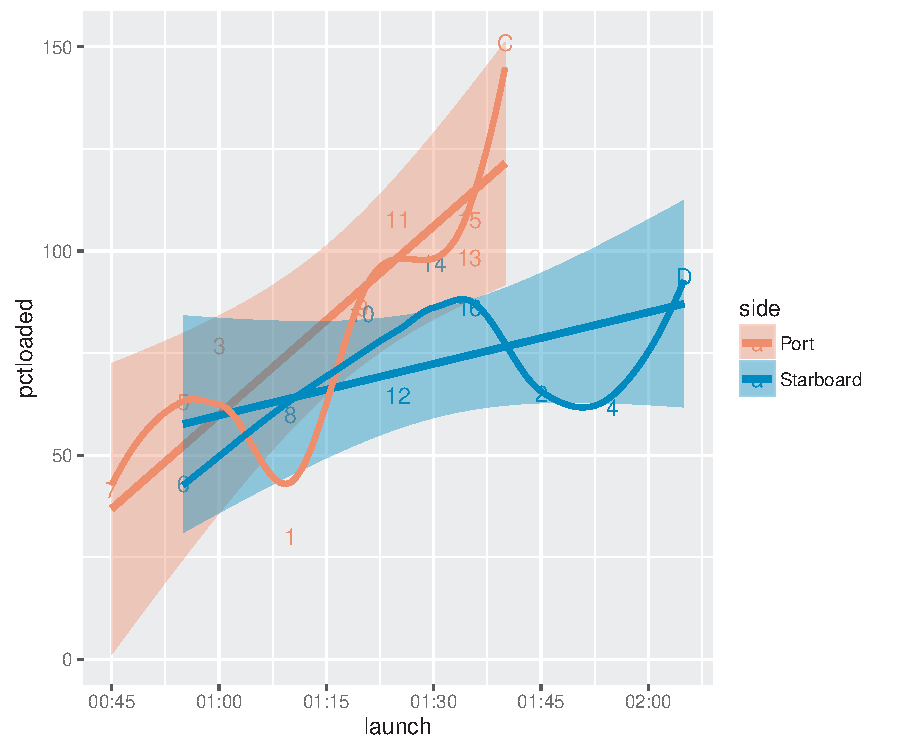
\includegraphics[width=.5\textwidth]{soln/fig/ex4_9b-1} }



\end{knitrout}
      Test a model allowing different slopes and intercepts for port and starboard sides:
\begin{knitrout}\footnotesize
\definecolor{shadecolor}{rgb}{0.941, 0.941, 0.941}\color{fgcolor}\begin{kframe}
\begin{alltt}
\hlstd{> }\hlkwd{summary}\hlstd{(}\hlkwd{lm}\hlstd{(pctloaded} \hlopt{~} \hlstd{side} \hlopt{*} \hlkwd{as.numeric}\hlstd{(launch),} \hlkwc{data}\hlstd{=Lifeboats))}
\end{alltt}
\begin{verbatim}

Call:
lm(formula = pctloaded ~ side * as.numeric(launch), data = Lifeboats)

Residuals:
   Min     1Q Median     3Q    Max 
-45.34 -11.78   0.34  11.46  29.61 

Coefficients:
                                  Estimate Std. Error t value Pr(>|t|)    
(Intercept)                       4.67e+07   1.10e+07    4.24  0.00083 ***
sideStarboard                    -3.39e+07   1.48e+07   -2.29  0.03800 *  
as.numeric(launch)                2.56e-02   6.05e-03    4.24  0.00083 ***
sideStarboard:as.numeric(launch) -1.86e-02   8.12e-03   -2.29  0.03800 *  
---
Signif. codes:  0 '***' 0.001 '**' 0.01 '*' 0.05 '.' 0.1 ' ' 1

Residual standard error: 20.2 on 14 degrees of freedom
Multiple R-squared:  0.602,	Adjusted R-squared:  0.517 
F-statistic: 7.06 on 3 and 14 DF,  p-value: 0.004
\end{verbatim}
\end{kframe}
\end{knitrout}
      \end{ans}
      
    \end{enumerate*}

\end{Exercises}

\clearpage
\chapter[Mosaic Displays for n-Way Tables]{Mosaic Displays for n-Way \mbox{Tables}}\label{ch:mosaic}


\begin{Exercises}

\exercise\label{lab:mosaic-criminal} The data set \data{criminal} in the package \pkg{logmult} gives the
$4 \times 5$ table below of the
number of men aged 15--19 charged with a criminal case for whom charges were dropped
in Denmark from 1955--1958.
\begin{knitrout}\footnotesize
\definecolor{shadecolor}{rgb}{0.941, 0.941, 0.941}\color{fgcolor}\begin{kframe}
\begin{alltt}
\hlstd{> }\hlkwd{data}\hlstd{(}\hlstr{"criminal"}\hlstd{,} \hlkwc{package} \hlstd{=} \hlstr{"logmult"}\hlstd{)}
\hlstd{> }\hlstd{criminal}
\end{alltt}
\begin{verbatim}
      Age
Year    15  16  17  18  19
  1955 141 285 320 441 427
  1956 144 292 342 441 396
  1957 196 380 424 462 427
  1958 212 424 399 442 430
\end{verbatim}
\end{kframe}
\end{knitrout}
  \begin{enumerate*}
    \item Use \func{loglm} to test whether there is an association between \var{Year}
    and \var{Age}.  Is there evidence that dropping of charges in relation to
    age changed over the years recorded here?
    \begin{ans}
    There is a significant association between \var{Year} and \var{Age}, so
    the row profiles of proportions differ over year.
\begin{knitrout}\footnotesize
\definecolor{shadecolor}{rgb}{0.941, 0.941, 0.941}\color{fgcolor}\begin{kframe}
\begin{alltt}
\hlstd{> }\hlkwd{loglm}\hlstd{(}\hlopt{~}\hlstd{Year} \hlopt{+} \hlstd{Age,} \hlkwc{data}\hlstd{=criminal)}
\end{alltt}
\begin{verbatim}
Call:
loglm(formula = ~Year + Age, data = criminal)

Statistics:
                    X^2 df   P(> X^2)
Likelihood Ratio 38.245 12 0.00014004
Pearson          38.410 12 0.00013155
\end{verbatim}
\end{kframe}
\end{knitrout}

    \end{ans}
    
    \item Use \func{mosaic} with the option \code{shade=TRUE} to display the
    pattern of signs and magnitudes of the residuals.  Compare this with the
    result of \func{mosaic} using ``Friendly shading,'' from
    the option \code{gp=shading\_Friendly}.  Describe verbally what you see
    in each regarding the pattern of association in this table.
    \begin{ans}
    It is helpful here to display all the residual contributions to association
    in the mosaic display using \code{labeling=labeling_residuals}.
\begin{knitrout}\footnotesize
\definecolor{shadecolor}{rgb}{0.941, 0.941, 0.941}\color{fgcolor}\begin{kframe}
\begin{alltt}
\hlstd{> }\hlkwd{mosaic}\hlstd{(criminal,} \hlkwc{shade}\hlstd{=}\hlnum{TRUE}\hlstd{,}
\hlstd{+ }       \hlkwc{labeling}\hlstd{=labeling_residuals,} \hlkwc{suppress}\hlstd{=}\hlnum{0}\hlstd{)}
\hlstd{> }\hlkwd{mosaic}\hlstd{(criminal,} \hlkwc{gp}\hlstd{=shading_Friendly,}
\hlstd{+ }       \hlkwc{labeling}\hlstd{=labeling_residuals,} \hlkwc{suppress}\hlstd{=}\hlnum{0}\hlstd{)}
\end{alltt}
\end{kframe}

\centerline{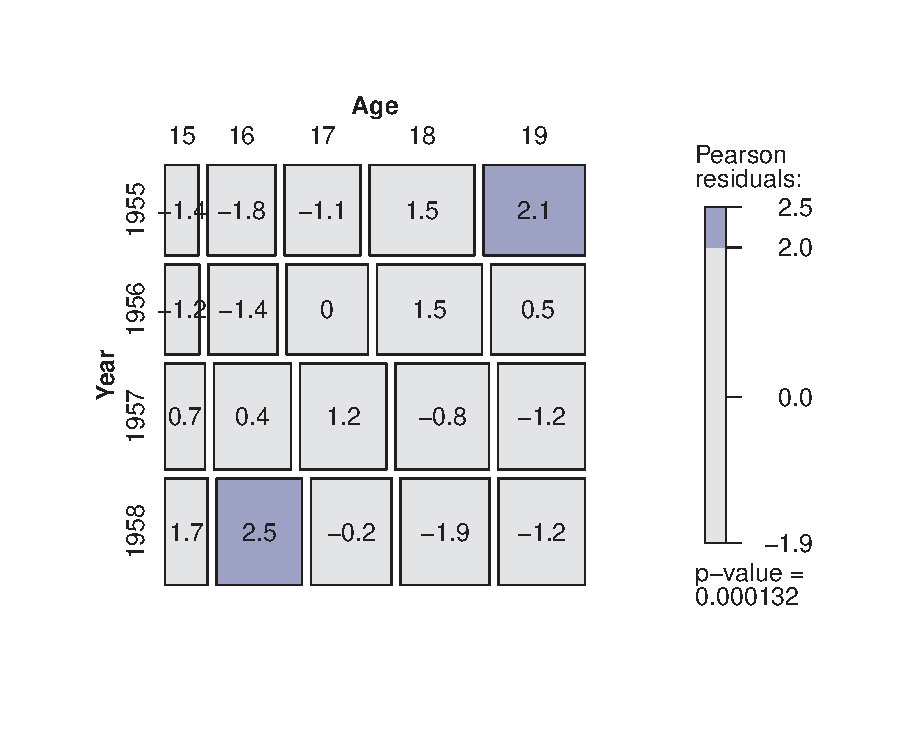
\includegraphics[width=.5\textwidth]{soln/fig/ex5_1b-1} 
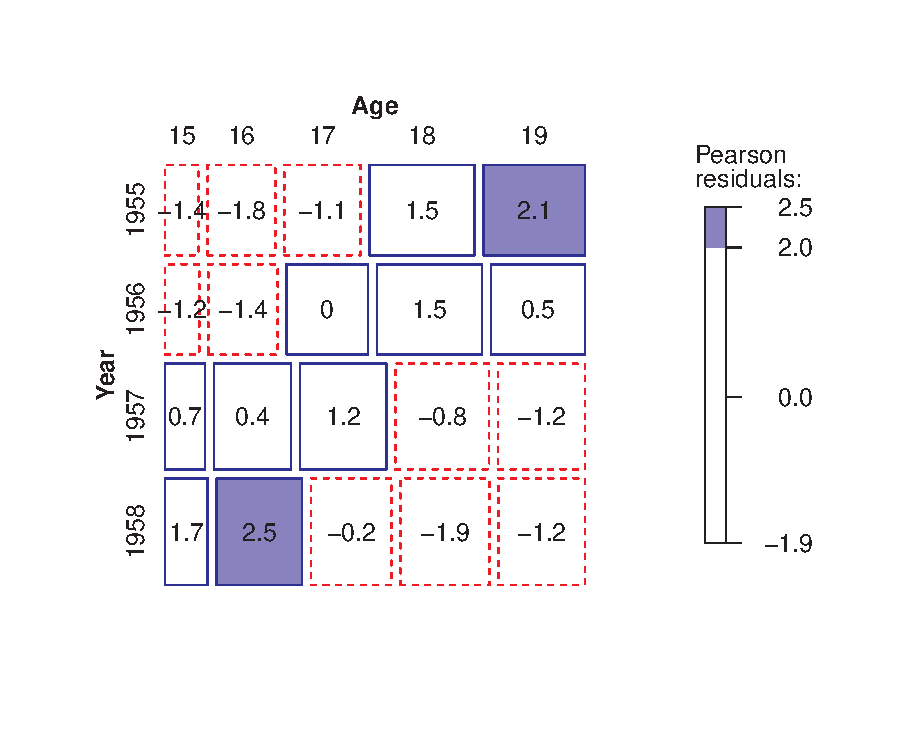
\includegraphics[width=.5\textwidth]{soln/fig/ex5_1b-2} }



\end{knitrout}
    Although only two residuals exceed the default $\vert r_{ij} \vert > 2$
    threshold for shading, there is clearly a systematic association between
    year and age shown by the signs of the residuals.
    
    The Friendly shading option here gives a better picture of the pattern of
    associations, showing positive and negative residuals in the diagonally
    opposite corners of the plot.  See \labref{lab:ca-criminal} for further
    analysis of this data.
    \end{ans}
    
  \end{enumerate*}

\exercise\label{lab:mosaic-crash} The data set \data{AirCrash} in \pkg{vcdExtra} gives a database of all crashes of commercial airplanes
between 1993--2015, classified by \var{Phase} of the flight and \var{Cause} of the crash.  How can you best show is the nature of the
association between these variables in a mosaic plot?  Start by making a frequency table, \code{aircrash.tab}:
\begin{knitrout}\footnotesize
\definecolor{shadecolor}{rgb}{0.941, 0.941, 0.941}\color{fgcolor}\begin{kframe}
\begin{alltt}
\hlstd{> }\hlkwd{data}\hlstd{(}\hlstr{"AirCrash"}\hlstd{,} \hlkwc{package} \hlstd{=} \hlstr{"vcdExtra"}\hlstd{)}
\hlstd{> }\hlstd{aircrash.tab} \hlkwb{<-} \hlkwd{xtabs}\hlstd{(}\hlopt{~} \hlstd{Phase} \hlopt{+} \hlstd{Cause,} \hlkwc{data} \hlstd{= AirCrash)}
\end{alltt}
\end{kframe}
\end{knitrout}
  \begin{enumerate*}
    \item Make a default mosaic display of the data with \code{shade=TRUE} and interpret the pattern of the high-frequency cells.
    \begin{ans}
\begin{knitrout}\footnotesize
\definecolor{shadecolor}{rgb}{0.941, 0.941, 0.941}\color{fgcolor}\begin{kframe}
\begin{alltt}
\hlstd{> } \hlkwd{mosaic}\hlstd{(aircrash.tab,} \hlkwc{shade}\hlstd{=}\hlnum{TRUE}\hlstd{)}
\end{alltt}
\end{kframe}

\centerline{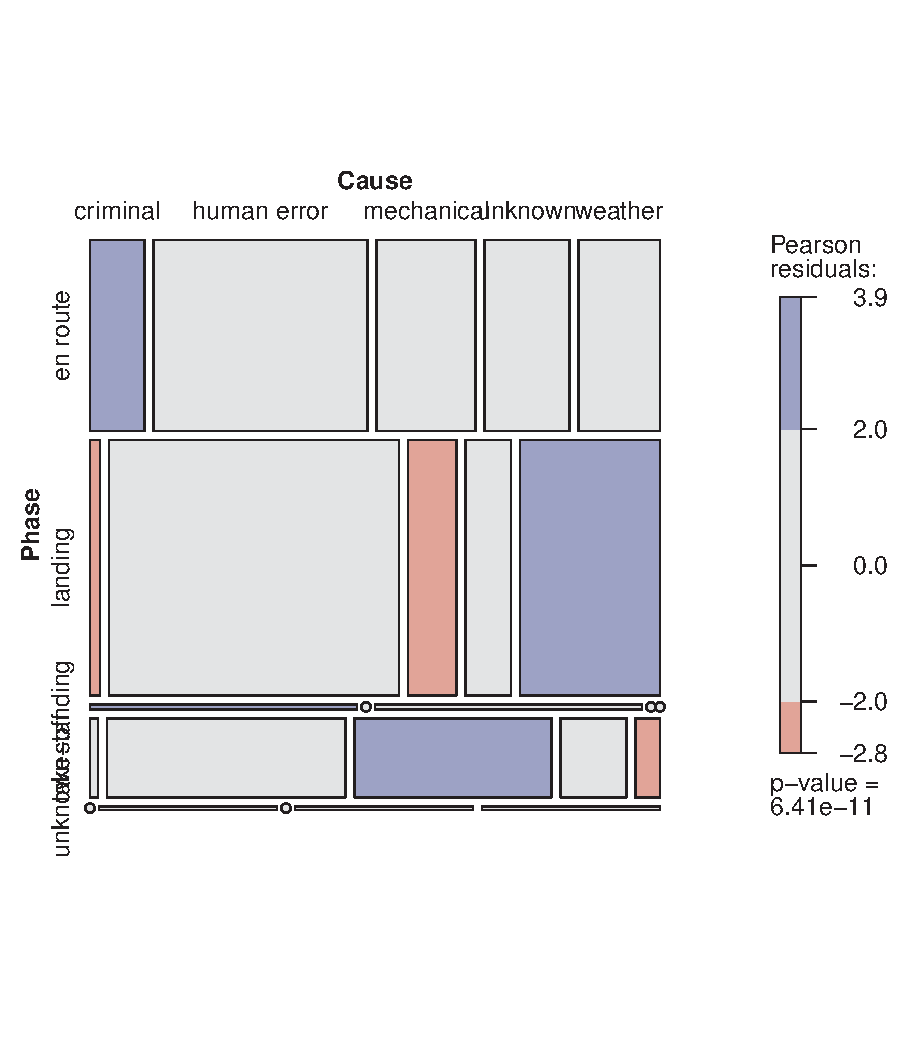
\includegraphics[width=0.5\textwidth]{soln/fig/ex5_2a-1} }



\end{knitrout}
    Four cells stand out as having greater than expected frequencies, if Phase and Cause were independent. 
    Both take-off and en-route are positively associated with criminal activities.
    Crashes in landing are more associated with weather.  It is difficult to interpret the unknown cells.
    \end{ans}
    
    
    \item The default plot has overlapping labels due to the uneven marginal frequencies relative to the lengths of the category
    labels.  Experiment with some of the \code{labeling\_args} options (\code{abbreviate}, \code{rot\_labels}, etc.)
    to see if you can make the plot more readable. \emph{Hint}: a variety of these are illustrated in \S 4.1 of \code{vignette("strucplot")}
    \begin{ans}
    Here are two alternatives that reduce the overplotting of labels:
\begin{knitrout}\footnotesize
\definecolor{shadecolor}{rgb}{0.941, 0.941, 0.941}\color{fgcolor}\begin{kframe}
\begin{alltt}
\hlstd{> }\hlkwd{mosaic}\hlstd{(aircrash.tab,} \hlkwc{shade}\hlstd{=}\hlnum{TRUE}\hlstd{,} \hlkwc{rot_labels}\hlstd{=}\hlkwd{c}\hlstd{(}\hlnum{20}\hlstd{,}\hlnum{90}\hlstd{,}\hlnum{0}\hlstd{,}\hlnum{70}\hlstd{),} \hlkwc{legend}\hlstd{=}\hlnum{FALSE}\hlstd{)}
\hlstd{> }\hlkwd{mosaic}\hlstd{(aircrash.tab,} \hlkwc{shade}\hlstd{=}\hlnum{TRUE}\hlstd{,} \hlkwc{alternate_labels}\hlstd{=}\hlnum{TRUE}\hlstd{,} \hlkwc{legend}\hlstd{=}\hlnum{FALSE}\hlstd{)}
\end{alltt}
\end{kframe}

\centerline{\includegraphics[width=.5\textwidth]{soln/fig/ex5_2b-1} 
\includegraphics[width=.5\textwidth]{soln/fig/ex5_2b-2} }



\end{knitrout}
    \end{ans}
    
    \item The levels of \var{Phase} and \var{Cause} are ordered alphabetically (because they are factors).  Experiment with 
    other orderings of the rows/columns to make interpretation clearer, e.g., ordering \var{Phase} temporally or ordering
    both factors by their marginal frequency.
    \begin{ans}
    Ordering by \var{Phase} is slightly easier to interpret.  Ordering both variables by marginal frequencies is
    also slightly better than the default, except that it leads to more overplotting of the labels.
\begin{knitrout}\footnotesize
\definecolor{shadecolor}{rgb}{0.941, 0.941, 0.941}\color{fgcolor}\begin{kframe}
\begin{alltt}
\hlstd{> }\hlcom{# reorder Phase temporarally}
\hlstd{> }\hlstd{roworder} \hlkwb{<-} \hlkwd{c}\hlstd{(}\hlnum{3}\hlstd{,} \hlnum{4}\hlstd{,} \hlnum{1}\hlstd{,} \hlnum{2}\hlstd{,} \hlnum{5}\hlstd{)}
\hlstd{> }\hlkwd{mosaic}\hlstd{(aircrash.tab[roworder,],} \hlkwc{shade}\hlstd{=}\hlnum{TRUE}\hlstd{,} \hlkwc{rot_labels}\hlstd{=}\hlkwd{c}\hlstd{(}\hlnum{20}\hlstd{,}\hlnum{90}\hlstd{,}\hlnum{0}\hlstd{,}\hlnum{70}\hlstd{),} \hlkwc{legend}\hlstd{=}\hlnum{FALSE}\hlstd{)}
\hlstd{> }
\hlstd{> }\hlcom{# marginal frequencies}
\hlstd{> }\hlstd{roworder} \hlkwb{<-} \hlkwd{order}\hlstd{(}\hlkwd{rowSums}\hlstd{(aircrash.tab))}
\hlstd{> }\hlstd{colorder} \hlkwb{<-} \hlkwd{order}\hlstd{(}\hlkwd{colSums}\hlstd{(aircrash.tab))}
\hlstd{> }\hlkwd{mosaic}\hlstd{(aircrash.tab[roworder, colorder],} \hlkwc{shade}\hlstd{=}\hlnum{TRUE}\hlstd{,} \hlkwc{rot_labels}\hlstd{=}\hlkwd{c}\hlstd{(}\hlnum{20}\hlstd{,}\hlnum{90}\hlstd{,}\hlnum{0}\hlstd{,}\hlnum{70}\hlstd{),} \hlkwc{legend}\hlstd{=}\hlnum{FALSE}\hlstd{)}
\end{alltt}
\end{kframe}

\centerline{\includegraphics[width=.5\textwidth]{soln/fig/ex5_2c-1} 
\includegraphics[width=.5\textwidth]{soln/fig/ex5_2c-2} }



\end{knitrout}
    The best general approach, as was illustrated in \figref{fig:glass-mosaic}, uses \term{effect ordering}
    to order the factors according to their associations.  One easy method for this \citep{FriendlyKwan:02:effect}
    is to order the factor levels according to their scores on the first dimension of a \ca solution
    as illustrated below.  This maximizes an opposite corner pattern of the residuals.
    
\begin{knitrout}\footnotesize
\definecolor{shadecolor}{rgb}{0.941, 0.941, 0.941}\color{fgcolor}\begin{kframe}
\begin{alltt}
\hlstd{> }\hlkwd{library}\hlstd{(ca)}
\hlstd{> }\hlstd{aircrash.ca} \hlkwb{<-} \hlkwd{ca}\hlstd{(aircrash.tab)}
\hlstd{> }\hlkwd{summary}\hlstd{(aircrash.ca,} \hlkwc{rows}\hlstd{=}\hlnum{FALSE}\hlstd{,} \hlkwc{columns}\hlstd{=}\hlnum{FALSE}\hlstd{)}
\end{alltt}
\begin{verbatim}

Principal inertias (eigenvalues):

 dim    value      %   cum%   scree plot               
 1      0.123002  65.6  65.6  ****************         
 2      0.051548  27.5  93.1  *******                  
 3      0.012340   6.6  99.7  **                       
 4      0.000562   0.3 100.0                           
        -------- -----                                 
 Total: 0.187452 100.0                                 
\end{verbatim}
\begin{alltt}
\hlstd{> }\hlcom{# reorder by CA coordinates on Dim 1}
\hlstd{> }\hlstd{roworder} \hlkwb{<-} \hlkwd{order}\hlstd{(aircrash.ca}\hlopt{$}\hlstd{rowcoord[,}\hlstr{"Dim1"}\hlstd{])}
\hlstd{> }\hlstd{colorder} \hlkwb{<-} \hlkwd{order}\hlstd{(aircrash.ca}\hlopt{$}\hlstd{colcoord[,}\hlstr{"Dim1"}\hlstd{])}
\hlstd{> }\hlstd{aircrash.tab[roworder, colorder]}
\end{alltt}
\begin{verbatim}
          Cause
Phase      criminal mechanical unknown human error weather
  standing        2          2       0           0       0
  take-off        1         24       8          29       3
  en route       16         29      25          63      24
  landing         4         19      18         114      55
  unknown         0          0       1           1       1
\end{verbatim}
\begin{alltt}
\hlstd{> }\hlkwd{mosaic}\hlstd{(aircrash.tab[roworder, colorder],} \hlkwc{shade}\hlstd{=}\hlnum{TRUE}\hlstd{,} \hlkwc{rot_labels}\hlstd{=}\hlkwd{c}\hlstd{(}\hlnum{20}\hlstd{,}\hlnum{90}\hlstd{,}\hlnum{0}\hlstd{,}\hlnum{70}\hlstd{))}
\end{alltt}
\end{kframe}

\centerline{\includegraphics[width=.5\textwidth]{soln/fig/ex5_2c2-1} }



\end{knitrout}
    
    \end{ans}
    
  \end{enumerate*}

\exercise The \Rpackage{Lahman} contains comprehensive data on baseball statistics for Major League Baseball from 1871 through 2012.  
For all players, the \data{Master} table records the handedness of players, in terms of
throwing (L, R) and batting (B, L, R), where B indicates ``both.''
The table below was generated using the following code:
\begin{knitrout}\footnotesize
\definecolor{shadecolor}{rgb}{0.941, 0.941, 0.941}\color{fgcolor}\begin{kframe}
\begin{alltt}
\hlstd{> }\hlkwd{library}\hlstd{(Lahman)}
\hlstd{> }\hlkwd{data}\hlstd{(}\hlstr{"Master"}\hlstd{,} \hlkwc{package} \hlstd{=} \hlstr{"Lahman"}\hlstd{)}
\hlstd{> }\hlstd{basehands} \hlkwb{<-} \hlkwd{with}\hlstd{(Master,} \hlkwd{table}\hlstd{(throws, bats))}
\end{alltt}
\end{kframe}
\end{knitrout}


% latex table generated in R 3.0.1 by xtable 1.7-1 package
% Thu Feb 27 12:56:12 2014
\begin{table}[ht]
\centering
\begin{tabular}{r|rrr}
  \hline
       & \multicolumn{3}{c}{Bats} \\
Throws & B & L & R \\ 
  \hline
  L & 177 & 2640 & 527 \\ 
  R & 924 & 1962 & 10442 \\ 
   \hline
\end{tabular}
\end{table}
  \begin{itemize*}
    \item Use the code above, or else enter these data into a frequency table in \R.
    \begin{ans}
    These notes use a later version of the Lahman package (v. 4.0-1) with the code above, so the numbers used in the plots
    don't correspond to those in the table.  The current version of the table is shown below.
\begin{knitrout}\footnotesize
\definecolor{shadecolor}{rgb}{0.941, 0.941, 0.941}\color{fgcolor}\begin{kframe}
\begin{alltt}
\hlstd{> }\hlstd{basehands}
\end{alltt}
\begin{verbatim}
      bats
throws     B     L     R
     L   182  2742   550
     R   956  2031 10814
\end{verbatim}
\end{kframe}
\end{knitrout}
    \end{ans}
    
    \item Construct mosaic displays showing the relation of batting and throwing handedness, split first by batting and then by throwing.
    \begin{ans}
    By default, a two-way \ctab is split first by the row variable, then by the column variable. 
    So, to split the other way, you can use \func{t} on the table argument.
\begin{knitrout}\footnotesize
\definecolor{shadecolor}{rgb}{0.941, 0.941, 0.941}\color{fgcolor}\begin{kframe}
\begin{alltt}
\hlstd{> }\hlkwd{mosaic}\hlstd{(basehands,} \hlkwc{shade}\hlstd{=}\hlnum{TRUE}\hlstd{,} \hlkwc{labeling}\hlstd{=}\hlkwd{labeling_residuals}\hlstd{(),} \hlkwc{legend}\hlstd{=}\hlnum{FALSE}\hlstd{)}
\hlstd{> }\hlkwd{mosaic}\hlstd{(}\hlkwd{t}\hlstd{(basehands),} \hlkwc{direction}\hlstd{=}\hlkwd{c}\hlstd{(}\hlstr{"h"}\hlstd{,} \hlstr{"v"}\hlstd{),} \hlkwc{shade}\hlstd{=}\hlnum{TRUE}\hlstd{,} \hlkwc{legend}\hlstd{=}\hlnum{FALSE}\hlstd{)}
\end{alltt}
\end{kframe}

\centerline{\includegraphics[width=.5\textwidth]{soln/fig/ex5_3b-1} 
\includegraphics[width=.5\textwidth]{soln/fig/ex5_3b-2} }



\end{knitrout}
    \end{ans}
    
    \item From these displays, what can be said about players who throw with their left
    or right hands in terms of their batting handedness?
    \begin{ans}
    Players who throw with their left or right hands are most likely to bat in the same way.
    From the values of the cell residuals, left handers are more likely to be uni-handers than
    righties.
    \end{ans}
    
  \end{itemize*}

\exercise\hard A related analysis concerns differences in throwing handedness among baseball players
according to the fielding position they play.  The following code calculates
such a frequency table.

\begin{knitrout}\footnotesize
\definecolor{shadecolor}{rgb}{0.941, 0.941, 0.941}\color{fgcolor}\begin{kframe}
\begin{alltt}
\hlstd{> }\hlkwd{library}\hlstd{(Lahman)}
\hlstd{> }\hlstd{MasterFielding} \hlkwb{<-} \hlkwd{data.frame}\hlstd{(}\hlkwd{merge}\hlstd{(Master, Fielding,} \hlkwc{by} \hlstd{=} \hlstr{"playerID"}\hlstd{))}
\hlstd{> }\hlstd{throwPOS} \hlkwb{<-} \hlkwd{with}\hlstd{(MasterFielding,} \hlkwd{table}\hlstd{(POS, throws))}
\end{alltt}
\end{kframe}
\end{knitrout}
  \begin{enumerate*}
    \item Make a mosaic display of throwing hand vs. fielding position.
    \begin{ans}
    There is clearly a very strong association between throwing hand and fielding position.
    A peculiarity of the data is that designated hitters (DH) do not 
    play a fielding position, but instead fill in for the pitcher in the batting order, so throwing
    hand is not really relevant here.  This position might arguably be deleted from this analysis.
\begin{knitrout}\footnotesize
\definecolor{shadecolor}{rgb}{0.941, 0.941, 0.941}\color{fgcolor}\begin{kframe}
\begin{alltt}
\hlstd{> }\hlkwd{mosaic}\hlstd{(throwPOS,} \hlkwc{shade}\hlstd{=}\hlnum{TRUE}\hlstd{,} \hlkwc{legend}\hlstd{=}\hlnum{FALSE}\hlstd{)}
\end{alltt}
\end{kframe}

\centerline{\includegraphics[width=.5\textwidth]{soln/fig/ex5_4a-1} }



\end{knitrout}
    \end{ans}
    
    \item Calculate the percentage of players throwing left-handed by position.
    Make a sensible graph of this data.
    \begin{ans}
    A barplot is simple and reasonable here. However, the levels of fielding position are
    ordered alphabetically, which makes interpretation harder. Sorting by \code{pctLeft}
    is better.
\begin{knitrout}\footnotesize
\definecolor{shadecolor}{rgb}{0.941, 0.941, 0.941}\color{fgcolor}\begin{kframe}
\begin{alltt}
\hlstd{> }\hlstd{pctLeft} \hlkwb{<-} \hlnum{100} \hlopt{*} \hlstd{throwPOS[,}\hlnum{1}\hlstd{]} \hlopt{/} \hlkwd{rowSums}\hlstd{(throwPOS)}
\hlstd{> }\hlstd{pctLeft}
\end{alltt}
\begin{verbatim}
    1B     2B     3B      C     CF     DH     LF     OF      P     RF     SS 
26.100  0.955  0.650  0.952 26.284 17.449 22.419 21.385 27.984 23.571  0.818 
\end{verbatim}
\begin{alltt}
\hlstd{> }\hlstd{ord} \hlkwb{<-} \hlkwd{order}\hlstd{(pctLeft)}
\hlstd{> }\hlkwd{barplot}\hlstd{(pctLeft,} \hlkwc{xlab}\hlstd{=}\hlstr{"Position"}\hlstd{,} \hlkwc{ylab}\hlstd{=}\hlstr{"Percent Left-handed"}\hlstd{)}
\hlstd{> }\hlkwd{barplot}\hlstd{(pctLeft[ord],} \hlkwc{xlab}\hlstd{=}\hlstr{"Position"}\hlstd{,} \hlkwc{ylab}\hlstd{=}\hlstr{"Percent Left-handed"}\hlstd{,} \hlkwc{col}\hlstd{=}\hlstr{"lightblue"}\hlstd{)}
\end{alltt}
\end{kframe}

\centerline{\includegraphics[width=.5\textwidth]{soln/fig/ex5_4b-1} 
\includegraphics[width=.5\textwidth]{soln/fig/ex5_4b-2} }



\end{knitrout}

    \end{ans}
    
    \item Re-do the mosaic display with the positions sorted by percentage of left-handers.
    \begin{ans}
\begin{knitrout}\footnotesize
\definecolor{shadecolor}{rgb}{0.941, 0.941, 0.941}\color{fgcolor}\begin{kframe}
\begin{alltt}
\hlstd{> }\hlkwd{mosaic}\hlstd{(throwPOS[ord,],} \hlkwc{shade}\hlstd{=}\hlnum{TRUE}\hlstd{,} \hlkwc{legend}\hlstd{=}\hlnum{FALSE}\hlstd{)}
\end{alltt}
\end{kframe}

\centerline{\includegraphics[width=.5\textwidth]{soln/fig/ex5_4c-1} }



\end{knitrout}
    \end{ans}
    
    \item Is there anything you can say about positions that have very few left-handed
    players?
    \begin{ans}
    All infield positions except for 1$^{st}$ base have a very small percentage of
    players who throw left-handed. Given the marginal distributions of handeness and
    position, outfielders, pitchers and 1$^{st}$ basemen are more likely to throw
    left-handed than if these variables were independent.
    \end{ans}
    
  \end{enumerate*}


\exercise For the \data{Bartlett} data described in \exref{ex:bartlett}, fit the model of no three-way
association, $H_4$ in \tabref{tab:hyp3way}. 
  \begin{enumerate*}
  
  \item Summarize the goodness of fit for this model, and compare to simpler models that
  omit one or more of the two-way terms.
  \begin{ans}
  \end{ans}
  
  
  \item Use a mosaic-like display to show the lack of fit for this model.
  \begin{ans}
  \end{ans}
  
  \end{enumerate*}

\exercise Red core disease, caused by a fungus, is not something you want if you are a strawberry.
The data set \data{jansen.strawberry} from the \Rpackage{agridat} gives a frequency data
frame of counts of damage from this fungus from a field experiment reported by
\cite{Jansen:1990}. See the help file for details.  The following lines create a
$3 \times 4 \times 3$ table of crossings of 3 male parents with 4 (different)
female parents, recording the number of plants in four blocks of 9 or 10 plants
each showing red core disease in three ordered categories, C1, C2, or C3.
\begin{knitrout}\footnotesize
\definecolor{shadecolor}{rgb}{0.941, 0.941, 0.941}\color{fgcolor}\begin{kframe}
\begin{alltt}
\hlstd{> }\hlkwd{data}\hlstd{(}\hlstr{"jansen.strawberry"}\hlstd{,} \hlkwc{package} \hlstd{=} \hlstr{"agridat"}\hlstd{)}
\hlstd{> }
\hlstd{> }\hlstd{dat} \hlkwb{<-} \hlstd{jansen.strawberry}
\hlstd{> }\hlstd{dat} \hlkwb{<-} \hlkwd{transform}\hlstd{(dat,} \hlkwc{category} \hlstd{=} \hlkwd{ordered}\hlstd{(category,}
\hlstd{+ }                                         \hlkwc{levels} \hlstd{=} \hlkwd{c}\hlstd{(}\hlstr{'C1'}\hlstd{,}\hlstr{'C2'}\hlstd{,}\hlstr{'C3'}\hlstd{)))}
\hlstd{> }\hlkwd{levels}\hlstd{(dat}\hlopt{$}\hlstd{male)} \hlkwb{<-} \hlkwd{paste0}\hlstd{(}\hlstr{"M"}\hlstd{,} \hlnum{1}\hlopt{:}\hlnum{3}\hlstd{)}
\hlstd{> }\hlkwd{levels}\hlstd{(dat}\hlopt{$}\hlstd{female)} \hlkwb{<-} \hlkwd{paste0}\hlstd{(}\hlstr{"F"}\hlstd{,} \hlnum{1}\hlopt{:}\hlnum{4}\hlstd{)}
\hlstd{> }
\hlstd{> }\hlstd{jansen.tab} \hlkwb{<-} \hlkwd{xtabs}\hlstd{(count} \hlopt{~} \hlstd{male} \hlopt{+} \hlstd{female} \hlopt{+} \hlstd{category,} \hlkwc{data} \hlstd{= dat)}
\hlstd{> }\hlkwd{names}\hlstd{(}\hlkwd{dimnames}\hlstd{(jansen.tab))} \hlkwb{<-} \hlkwd{c}\hlstd{(}\hlstr{"Male parent"}\hlstd{,} \hlstr{"Female parent"}\hlstd{,}
\hlstd{+ }                                 \hlstr{"Disease category"}\hlstd{)}
\hlstd{> }\hlkwd{ftable}\hlstd{(jansen.tab)}
\end{alltt}
\begin{verbatim}
                          Disease category C1 C2 C3
Male parent Female parent                          
M1          F1                              6 13 20
            F2                              8 15 17
            F3                             13 10 16
            F4                              8 21 11
M2          F1                              5 13 21
            F2                              9 16 14
            F3                             16  9 15
            F4                             12 13 14
M3          F1                              5 10 24
            F2                             13 12 15
            F3                              3 14 22
            F4                             18  9 13
\end{verbatim}
\end{kframe}
\end{knitrout}
  \begin{enumerate*}
    \item Use \code{pairs(jansen.tab, shade=TRUE)} to display the pairwise associations
    among the three variables.  Describe how disease category appears to vary with male
    and female parent. Why is there no apparent association between male and female parent?
    \begin{ans}
    This was a designed experiment, with male and female parents completely crossed
    to create 12 populations.
    Disease categories seem to be associated with female parents, with more serious
    disease (C3) more prevalent in parent F4.
\begin{knitrout}\footnotesize
\definecolor{shadecolor}{rgb}{0.941, 0.941, 0.941}\color{fgcolor}\begin{kframe}
\begin{alltt}
\hlstd{> }\hlkwd{library}\hlstd{(vcd)}
\hlstd{> }\hlkwd{pairs}\hlstd{(jansen.tab,} \hlkwc{shade}\hlstd{=}\hlnum{TRUE}\hlstd{)}
\end{alltt}
\end{kframe}

\centerline{\includegraphics[width=.6\textwidth]{soln/fig/ex5_6a-1} }



\end{knitrout}
    \end{ans}
    
    \item As illustrated in \figref{fig:HE-fill}, use \func{mosaic} to prepare a 3-way mosaic
    plot with the tiles colored in increasing shades of some color according to
    disease category.  Describe the pattern of category C3 in relation to male and
    female parent.  (Hint: the \code{highlighting} arguments are useful here.)
    \begin{ans}
\begin{knitrout}\footnotesize
\definecolor{shadecolor}{rgb}{0.941, 0.941, 0.941}\color{fgcolor}\begin{kframe}
\begin{alltt}
\hlstd{> }\hlstd{cols} \hlkwb{<-} \hlkwd{c}\hlstd{(}\hlstr{"moccasin"}\hlstd{,}\hlstr{"lightsalmon1"}\hlstd{,}\hlstr{"indianred"}\hlstd{)}
\hlstd{> }\hlkwd{mosaic}\hlstd{(jansen.tab,} \hlkwc{highlighting}\hlstd{=}\hlnum{3}\hlstd{,} \hlkwc{highlighting_fill}\hlstd{=cols)}
\end{alltt}
\end{kframe}

\centerline{\includegraphics[width=.5\textwidth]{soln/fig/ex5_6b-1} }



\end{knitrout}
    \end{ans}
    
    \item With \code{category} as the response variable, the minimal model for
    association is \LLM{MF,C}, or \verb|~ 1*2 + 3|.
    Fit this model using \func{loglm} and display the residuals from this model
    with \func{mosaic}. Describe the pattern of lack of fit of this model.
    \begin{ans}
\begin{knitrout}\footnotesize
\definecolor{shadecolor}{rgb}{0.941, 0.941, 0.941}\color{fgcolor}\begin{kframe}
\begin{alltt}
\hlstd{> }\hlcom{# baseline model}
\hlstd{> }\hlkwd{library}\hlstd{(MASS)}
\hlstd{> }\hlkwd{loglm}\hlstd{(}\hlopt{~}\hlnum{1}\hlopt{*}\hlnum{2}\hlopt{+}\hlnum{3}\hlstd{,}\hlkwc{data}\hlstd{=jansen.tab)}
\end{alltt}
\begin{verbatim}
Call:
loglm(formula = ~1 * 2 + 3, data = jansen.tab)

Statistics:
                   X^2 df  P(> X^2)
Likelihood Ratio 45.63 22 0.0022062
Pearson          45.65 22 0.0021927
\end{verbatim}
\begin{alltt}
\hlstd{> }\hlkwd{mosaic}\hlstd{(jansen.tab,} \hlkwc{expected} \hlstd{=} \hlopt{~} \hlnum{1}\hlopt{*}\hlnum{2}\hlopt{+}\hlnum{3}\hlstd{)}
\end{alltt}
\end{kframe}

\centerline{\includegraphics[width=.5\textwidth]{soln/fig/ex5_6c-1} }



\end{knitrout}

    \end{ans}
    
  \end{enumerate*}

  \exercise The data set \data{caith} in \pkg{MASS} gives another
  classic $4 \times 5$ table 
  tabulating hair color and eye color, this for  
  people in Caithness, Scotland, originally from
  \citet{Fisher:1940}.  The data is stored as a data frame of cell frequencies, whose rows are eye colors
  and whose columns are hair colors.
\begin{knitrout}\footnotesize
\definecolor{shadecolor}{rgb}{0.941, 0.941, 0.941}\color{fgcolor}\begin{kframe}
\begin{alltt}
\hlstd{> }\hlkwd{data}\hlstd{(}\hlstr{"caith"}\hlstd{,} \hlkwc{package} \hlstd{=} \hlstr{"MASS"}\hlstd{)}
\hlstd{> }\hlstd{caith}
\end{alltt}
\begin{verbatim}
       fair red medium dark black
blue    326  38    241  110     3
light   688 116    584  188     4
medium  343  84    909  412    26
dark     98  48    403  681    85
\end{verbatim}
\end{kframe}
\end{knitrout}

  \begin{enumerate*}
    \item The \func{loglm} and \func{mosaic} functions don't understand data in this format, 
    so use \code{Caith <- as.matrix(caith)} 
    to convert to array form.  Examine the result, and use \code{names(dimnames(Caith))<-c()} to %%isolated newline hack
    assign appropriate names to the row and column dimensions.
    \begin{ans}
\begin{knitrout}\footnotesize
\definecolor{shadecolor}{rgb}{0.941, 0.941, 0.941}\color{fgcolor}\begin{kframe}
\begin{alltt}
\hlstd{> }\hlstd{Caith} \hlkwb{<-} \hlkwd{as.matrix}\hlstd{(caith)}
\hlstd{> }\hlkwd{dimnames}\hlstd{(Caith)}
\end{alltt}
\begin{verbatim}
[[1]]
[1] "blue"   "light"  "medium" "dark"  

[[2]]
[1] "fair"   "red"    "medium" "dark"   "black" 
\end{verbatim}
\begin{alltt}
\hlstd{> }\hlkwd{names}\hlstd{(}\hlkwd{dimnames}\hlstd{(Caith))} \hlkwb{<-} \hlkwd{c}\hlstd{(}\hlstr{"Eye"}\hlstd{,} \hlstr{"Hair"}\hlstd{)}
\end{alltt}
\end{kframe}
\end{knitrout}
    \end{ans}
    
    \item Fit the model of independence to the resulting matrix using \func{loglm}.
    \begin{ans}
\begin{knitrout}\footnotesize
\definecolor{shadecolor}{rgb}{0.941, 0.941, 0.941}\color{fgcolor}\begin{kframe}
\begin{alltt}
\hlstd{> }\hlstd{(caith.mod} \hlkwb{<-} \hlkwd{loglm}\hlstd{(}\hlopt{~}\hlstd{Hair}\hlopt{+}\hlstd{Eye,} \hlkwc{data}\hlstd{=Caith,} \hlkwc{fitted}\hlstd{=}\hlnum{TRUE}\hlstd{))}
\end{alltt}
\begin{verbatim}
Call:
loglm(formula = ~Hair + Eye, data = Caith, fitted = TRUE)

Statistics:
                    X^2 df P(> X^2)
Likelihood Ratio 1218.3 12        0
Pearson          1240.0 12        0
\end{verbatim}
\end{kframe}
\end{knitrout}
    \end{ans}
    
    
    \item Calculate and display the residuals for this model.
    \begin{ans}
\begin{knitrout}\footnotesize
\definecolor{shadecolor}{rgb}{0.941, 0.941, 0.941}\color{fgcolor}\begin{kframe}
\begin{alltt}
\hlstd{> }\hlkwd{residuals}\hlstd{(caith.mod)}
\end{alltt}
\begin{verbatim}
        Hair
Eye        fair     red medium   dark black
  blue     8.63 -0.0193  -2.67  -6.00 -3.94
  light   11.60  3.3125  -1.73 -12.19 -6.63
  medium  -6.56 -1.0691   7.40  -2.19 -2.20
  dark   -16.19 -2.7683  -5.41  16.28  8.46
\end{verbatim}
\end{kframe}
\end{knitrout}
    \end{ans}
    
    \item Create a mosaic display for this data.
    \begin{ans}
\begin{knitrout}\footnotesize
\definecolor{shadecolor}{rgb}{0.941, 0.941, 0.941}\color{fgcolor}\begin{kframe}
\begin{alltt}
\hlstd{> }\hlkwd{mosaic}\hlstd{(Caith,} \hlkwc{shade}\hlstd{=}\hlnum{TRUE}\hlstd{)}
\end{alltt}
\end{kframe}

\centerline{\includegraphics[width=.6\textwidth]{soln/fig/ex5_7d-1} }



\end{knitrout}

    \end{ans}
    
  \end{enumerate*}
  
%\TODO{Add exercise using \code{vcd::HairEyePlace}}

  \exercise The \data{HairEyePlace} data in \pkg{vcdExtra} gives similar data on hair color and eye color, for both
  Caithness and Aberdeen as a $4 \times 5 \times 2$ table.
  \begin{enumerate*}
    \item Prepare separate mosaic displays, one for each of Caithness and Aberdeen.  Comment on any difference in
    the pattern of residuals.
    \begin{ans}
    \end{ans}
    
    \item Construct conditional mosaic plots, using the formula
      \verb/~ Hair + Eye | Place/ and both \func{mosaic} and
    \func{cotabplot}. It is probably more useful here to suppress the legend in these plots.  Comment on the
    difference in what is shown in the two displays.
    \begin{ans}
    \end{ans}
    
  \end{enumerate*}
  

  \exercise\label{lab:mosaic-accident} \citet[pp. 30--31]{Bertin:83} used a 4-way table of frequencies of traffic accident victims in France in 1958
  to illustrate his scheme for classifying data sets by numerous variables, each of which could have various types
  and could be assigned to various visual attributes. His data are contained in \data{Accident} in \pkg{vcdExtra},
  a frequency data frame representing his $5 \times 2 \times 4 \times 2$ table of the variables
  \var{age}, \var{result} (died or injured), \var{mode} of transportation, and \var{gender}.
\begin{knitrout}\footnotesize
\definecolor{shadecolor}{rgb}{0.941, 0.941, 0.941}\color{fgcolor}\begin{kframe}
\begin{alltt}
\hlstd{> }\hlkwd{data}\hlstd{(}\hlstr{"Accident"}\hlstd{,} \hlkwc{package} \hlstd{=} \hlstr{"vcdExtra"}\hlstd{)}
\hlstd{> }\hlkwd{str}\hlstd{(Accident,} \hlkwc{vec.len}\hlstd{=}\hlnum{2}\hlstd{)}
\end{alltt}
\begin{verbatim}
'data.frame':	80 obs. of  5 variables:
 $ age   : Ord.factor w/ 5 levels "0-9"<"10-19"<..: 5 5 5 5 5 ...
 $ result: Factor w/ 2 levels "Died","Injured": 1 1 1 1 1 ...
 $ mode  : Factor w/ 4 levels "4-Wheeled","Bicycle",..: 4 4 2 2 3 ...
 $ gender: Factor w/ 2 levels "Female","Male": 2 1 2 1 2 ...
 $ Freq  : int  704 378 396 56 742 ...
\end{verbatim}
\end{kframe}
\end{knitrout}
    \begin{enumerate*}
    
      \item Use \func{loglm} to fit the model of mutual independence, \verb|Freq ~ age+mode+gender+result| to
      this data set.
      \begin{ans}
      You can use \func{loglm} directly on the frequency data frame, with \code{Freq} as the response:
\begin{knitrout}\footnotesize
\definecolor{shadecolor}{rgb}{0.941, 0.941, 0.941}\color{fgcolor}\begin{kframe}
\begin{alltt}
\hlstd{> }\hlkwd{library}\hlstd{(MASS)}
\hlstd{> }\hlkwd{loglm}\hlstd{(Freq} \hlopt{~} \hlstd{age} \hlopt{+} \hlstd{mode} \hlopt{+} \hlstd{gender} \hlopt{+} \hlstd{result,} \hlkwc{data} \hlstd{= Accident)}
\end{alltt}
\begin{verbatim}
Call:
loglm(formula = Freq ~ age + mode + gender + result, data = Accident)

Statistics:
                   X^2 df P(> X^2)
Likelihood Ratio 60320 70        0
Pearson          76865 70        0
\end{verbatim}
\end{kframe}
\end{knitrout}
      Or, convert to an array first with \func{xtabs}
\begin{knitrout}\footnotesize
\definecolor{shadecolor}{rgb}{0.941, 0.941, 0.941}\color{fgcolor}\begin{kframe}
\begin{alltt}
\hlstd{> }\hlstd{accident.tab} \hlkwb{<-} \hlkwd{xtabs}\hlstd{(Freq} \hlopt{~} \hlstd{age} \hlopt{+} \hlstd{mode} \hlopt{+} \hlstd{gender} \hlopt{+} \hlstd{result,} \hlkwc{data} \hlstd{= Accident)}
\hlstd{> }\hlkwd{loglm}\hlstd{(}\hlopt{~} \hlstd{age} \hlopt{+} \hlstd{mode} \hlopt{+} \hlstd{gender} \hlopt{+} \hlstd{result,} \hlkwc{data} \hlstd{= accident.tab)}
\end{alltt}
\begin{verbatim}
Call:
loglm(formula = ~age + mode + gender + result, data = accident.tab)

Statistics:
                   X^2 df P(> X^2)
Likelihood Ratio 60320 70        0
Pearson          76865 70        0
\end{verbatim}
\end{kframe}
\end{knitrout}
      \end{ans}
      
      \item Use \func{mosaic} to produce an interpretable mosaic plot of the associations among all variables under the
      model of mutual independence.  Try different orders of the variables in the mosaic.  (\emph{Hint}: the 
      \code{abbreviate} component of the 
      \code{labeling\_args} argument to \func{mosaic} will be useful to avoid some overlap of the category labels.)
      \begin{ans}
      In this data set, \code{mode} is arguably an ordered factor, and better results will come from reordering
      its levels, from Pedestrian to 4-Wheeled vehicle.
      The order of variables given in \func{xtabs} gives a reasonable result.  The label overlap can be avoided
      by rotating the labels for \code{mode}.
\begin{knitrout}\footnotesize
\definecolor{shadecolor}{rgb}{0.941, 0.941, 0.941}\color{fgcolor}\begin{kframe}
\begin{alltt}
\hlstd{> }\hlstd{Accident}\hlopt{$}\hlstd{mode} \hlkwb{<-} \hlkwd{ordered}\hlstd{(Accident}\hlopt{$}\hlstd{mode,}
\hlstd{+ }   \hlkwc{levels}\hlstd{=}\hlkwd{levels}\hlstd{(Accident}\hlopt{$}\hlstd{mode)[}\hlkwd{c}\hlstd{(}\hlnum{4}\hlstd{,}\hlnum{2}\hlstd{,}\hlnum{3}\hlstd{,}\hlnum{1}\hlstd{)])}
\hlstd{> }\hlkwd{mosaic}\hlstd{(accident.tab,} \hlkwc{shade}\hlstd{=}\hlnum{TRUE}\hlstd{,} \hlkwc{rot_labels} \hlstd{=} \hlkwd{c}\hlstd{(}\hlnum{20}\hlstd{,} \hlnum{90}\hlstd{,} \hlnum{00}\hlstd{,} \hlnum{90}\hlstd{))}
\end{alltt}
\end{kframe}

\centerline{\includegraphics[width=.6\textwidth]{soln/fig/ex5_9b-1} }



\end{knitrout}
      \end{ans}
      
      \item Treat \var{result} (\code{"Died"} vs. \code{"Injured"}) as the response variable, and fit the model \newline
      \verb|Freq ~ age*mode*gender + result| that asserts independence of \var{result} from all others jointly.
      \begin{ans}
      This fits much better than the mutual independence model, but still has a terrible fit.
      There still remain important associations between \code{result} and the other variables
\begin{knitrout}\footnotesize
\definecolor{shadecolor}{rgb}{0.941, 0.941, 0.941}\color{fgcolor}\begin{kframe}
\begin{alltt}
\hlstd{> }\hlkwd{loglm}\hlstd{(Freq} \hlopt{~} \hlstd{age} \hlopt{*} \hlstd{mode} \hlopt{*} \hlstd{gender} \hlopt{+} \hlstd{result,} \hlkwc{data} \hlstd{= Accident)}
\end{alltt}
\begin{verbatim}
Call:
loglm(formula = Freq ~ age * mode * gender + result, data = Accident)

Statistics:
                    X^2 df P(> X^2)
Likelihood Ratio 2217.7 39        0
Pearson          2347.6 39        0
\end{verbatim}
\end{kframe}
\end{knitrout}
      \end{ans}
      
      \item Construct a mosaic display for the residual associations in this model.  Which combinations of the
      predictor factors are more likely to result in death?
      \begin{ans}
      The largest postive residuals appear in the 50+ age group, where males are more likely to have died,
      regardless of \code{mode}.  It can also be seen that in the 30--49 age group, more males die
      in bicycle and motorcycle accidents.  Other permutations of the table variables or
      other displays like doubledecker plots can highlight other features.
\begin{knitrout}\footnotesize
\definecolor{shadecolor}{rgb}{0.941, 0.941, 0.941}\color{fgcolor}\begin{kframe}
\begin{alltt}
\hlstd{> }\hlkwd{mosaic}\hlstd{(accident.tab,} \hlkwc{expected} \hlstd{=} \hlopt{~}\hlstd{age} \hlopt{*} \hlstd{mode} \hlopt{*} \hlstd{gender} \hlopt{+} \hlstd{result,}
\hlstd{+ }       \hlkwc{shade}\hlstd{=}\hlnum{TRUE}\hlstd{,} \hlkwc{rot_labels} \hlstd{=} \hlkwd{c}\hlstd{(}\hlnum{20}\hlstd{,} \hlnum{90}\hlstd{,} \hlnum{00}\hlstd{,} \hlnum{90}\hlstd{),}
\hlstd{+ }       \hlkwc{gp_args}\hlstd{=}\hlkwd{list}\hlstd{(}\hlkwc{interpolate}\hlstd{=}\hlkwd{c}\hlstd{(}\hlnum{1}\hlstd{,}\hlnum{2}\hlstd{,}\hlnum{4}\hlstd{,}\hlnum{8}\hlstd{)))}
\end{alltt}
\end{kframe}

\centerline{\includegraphics[width=.6\textwidth]{soln/fig/ex5_9d-1} }



\end{knitrout}
      \end{ans}
      
    \end{enumerate*}

  \exercise\label{lab:mosaic-vietnam}The data set \data{Vietnam} in \pkg{vcdExtra} gives a $2 \times 5 \times 4$ contingency table in frequency form reflecting a survey of student opinion on the Vietnam War at the University of North Carolina in May 1967.  
  The table variables are sex, year in school, and response, which has categories: (A) Defeat North Vietnam by widespread bombing and land invasion; (B) Maintain the present policy; (C) De-escalate military activity, stop bombing and begin negotiations; (D) Withdraw military forces immediately.  How does the chosen response vary with sex and year?
\begin{knitrout}\footnotesize
\definecolor{shadecolor}{rgb}{0.941, 0.941, 0.941}\color{fgcolor}\begin{kframe}
\begin{alltt}
\hlstd{> }\hlkwd{data}\hlstd{(}\hlstr{"Vietnam"}\hlstd{,} \hlkwc{package} \hlstd{=} \hlstr{"vcdExtra"}\hlstd{)}
\hlstd{> }\hlkwd{str}\hlstd{(Vietnam)}
\end{alltt}
\begin{verbatim}
'data.frame':	40 obs. of  4 variables:
 $ sex     : Factor w/ 2 levels "Female","Male": 1 1 1 1 1 1 1 1 1 1 ...
 $ year    : int  1 1 1 1 2 2 2 2 3 3 ...
 $ response: Factor w/ 4 levels "A","B","C","D": 1 2 3 4 1 2 3 4 1 2 ...
 $ Freq    : int  13 19 40 5 5 9 33 3 22 29 ...
\end{verbatim}
\end{kframe}
\end{knitrout}
    \begin{enumerate*}
      \item With \var{response} (R) as the outcome variable and \var{year} (Y) and \var{sex} (S) as predictors, the minimal
      baseline \loglin model is the model of joint independence, \LLM{R,YS}.  Fit this model, and display it in
      a mosaic plot.
      \begin{ans}
      The baseline model does not fit well, so \var{response} is associated with either \var{year} or \var{sex}
      or both.  Note that when fitting with \func{loglm} (or \func{glm}), both \code{mosaic(mod)} and \code{plot(mod)}
      give the corresponding mosaic plot for a model object, \code{mod}.
\begin{knitrout}\footnotesize
\definecolor{shadecolor}{rgb}{0.941, 0.941, 0.941}\color{fgcolor}\begin{kframe}
\begin{alltt}
\hlstd{> }\hlkwd{library}\hlstd{(MASS)}
\hlstd{> }\hlkwd{library}\hlstd{(vcdExtra)}
\hlstd{> }\hlstd{(viet.mod} \hlkwb{<-} \hlkwd{loglm}\hlstd{(Freq} \hlopt{~} \hlstd{sex} \hlopt{*} \hlstd{year} \hlopt{+} \hlstd{response,} \hlkwc{data}\hlstd{=Vietnam))}
\end{alltt}
\begin{verbatim}
Call:
loglm(formula = Freq ~ sex * year + response, data = Vietnam)

Statistics:
                    X^2 df P(> X^2)
Likelihood Ratio 361.72 27        0
Pearson          366.36 27        0
\end{verbatim}
\begin{alltt}
\hlstd{> }\hlkwd{mosaic}\hlstd{(viet.mod)}
\hlstd{> }\hlcom{# plot(viet.mod)     # same}
\end{alltt}
\end{kframe}

\centerline{\includegraphics[width=.5\textwidth]{soln/fig/ex5_10a-1} }



\end{knitrout}

      \end{ans}
      
      \item Construct conditional mosaic plots of the \var{response} versus \var{year} separately for males and females.
      Describe the associations seen here.
      \begin{ans}
      We use \func{cotabplot} here, with the formula \verb|~ response + year | sex| to condition on sex.
      For males, there is a clear association between response and year, with 1$^{st}$ year students prefering
      the more military response A, and later-year students tending toward the more peaceful response D.
      For females, the association between response and year is weak, and does not show a coherent pattern.
\begin{knitrout}\footnotesize
\definecolor{shadecolor}{rgb}{0.941, 0.941, 0.941}\color{fgcolor}\begin{kframe}
\begin{alltt}
\hlstd{> }\hlkwd{cotabplot}\hlstd{(}\hlopt{~} \hlstd{response} \hlopt{+} \hlstd{year} \hlopt{|} \hlstd{sex,} \hlkwc{data}\hlstd{=vietnam.tab,}
\hlstd{+ }                                  \hlkwc{gp}\hlstd{=shading_Friendly,} \hlkwc{gp_args}\hlstd{=}\hlkwd{list}\hlstd{(}\hlkwc{interpolate}\hlstd{=}\hlnum{1}\hlopt{:}\hlnum{4}\hlstd{),} \hlkwc{legend}\hlstd{=}\hlnum{FALSE}\hlstd{)}
\end{alltt}
\end{kframe}

\centerline{\includegraphics[width=.8\textwidth]{soln/fig/ex5_10b-1} }



\end{knitrout}

      \end{ans}
      
      \item Follow the methods shown in \exref{ex:employ} to fit separate models of independence for the levels of \var{sex},
      and the model of conditional independence, $R \perp Y \given S$.
      Verify that the decomposition of $\GSQ$ in \eqref{eq:partial1} holds for these models.
      \begin{ans}
      Splitting the data by sex, using \func{apply} shows that the association between response and year is
      strongly significant for males, but not for females. 
\begin{knitrout}\footnotesize
\definecolor{shadecolor}{rgb}{0.941, 0.941, 0.941}\color{fgcolor}\begin{kframe}
\begin{alltt}
\hlstd{> }\hlstd{mods.list} \hlkwb{<-}
\hlstd{+ }        \hlkwd{apply}\hlstd{(vietnam.tab,} \hlstr{"sex"}\hlstd{,}
\hlstd{+ }              \hlkwa{function}\hlstd{(}\hlkwc{x}\hlstd{)} \hlkwd{loglm}\hlstd{(}\hlopt{~} \hlstd{response} \hlopt{+} \hlstd{year,} \hlkwc{data}\hlstd{=x))}
\hlstd{> }\hlstd{mods.list}
\end{alltt}
\begin{verbatim}
$Female
Call:
loglm(formula = ~response + year, data = x)

Statistics:
                    X^2 df P(> X^2)
Likelihood Ratio 13.263 12  0.35022
Pearson          13.294 12  0.34803

$Male
Call:
loglm(formula = ~response + year, data = x)

Statistics:
                    X^2 df P(> X^2)
Likelihood Ratio 203.05 12        0
Pearson          198.50 12        0
\end{verbatim}
\end{kframe}
\end{knitrout}
      \end{ans}
      
      \item Construct a useful 3-way mosaic plot of the data for the model of conditional independence.
      \begin{ans}
      \end{ans}
      
    \end{enumerate*}

\exercise Consider the models for 4-way tables shown in \tabref{tab:seqmodels}. 
  \begin{enumerate*}
    \item For each model, give an independence interpretation.  For example, the model of mutual
    independence corresponds to $A \perp B \perp C \perp D$.
    \begin{ans}
    The basic idea of the notation is that terms in separate []s are said to be independent
    under a given model. Variables within a [] term are allowed to be associated
    \begin{itemize*}
      \item mutual: [A]  [B]  [C]  [D] $\leftrightarrow A \perp B \perp C \perp D$
      \item joint: [ABC]  [D] $\leftrightarrow (ABC) \perp D$
      \item conditional: [AD]  [BD]  [CD] $\leftrightarrow (AD) \perp (BD) \perp (CD)$
      \item markov (order 1): [AB]  [BC]  [CD] $\leftrightarrow (AB) \perp (BC) \perp (CD)$
      \item markov (order 2): [ABC]  [BCD] $\leftrightarrow (ABC) \perp (BCD)$
      \item saturated: no independence relationship
    \end{itemize*}
    \end{ans}
    
    \item Use the functions shown in the table together with \func{loglin2formula} to print the
    corresponding model formulas for each.
    \begin{ans}
    The model generating functions, \func{mutual}, \func{joint}, etc. provide a simple way to
    specify loglinear models for \func{loglm} and \func{mosaic}.  
\begin{knitrout}\footnotesize
\definecolor{shadecolor}{rgb}{0.941, 0.941, 0.941}\color{fgcolor}\begin{kframe}
\begin{alltt}
\hlstd{> }\hlkwd{loglin2formula}\hlstd{(}\hlkwd{mutual}\hlstd{(}\hlnum{4}\hlstd{,} \hlkwc{factors}\hlstd{=LETTERS[}\hlnum{1}\hlopt{:}\hlnum{4}\hlstd{]))}
\end{alltt}
\begin{verbatim}
~A + B + C + D
\end{verbatim}
\begin{alltt}
\hlstd{> }\hlkwd{loglin2formula}\hlstd{(}\hlkwd{joint}\hlstd{(}\hlnum{4}\hlstd{,} \hlkwc{factors}\hlstd{=LETTERS[}\hlnum{1}\hlopt{:}\hlnum{4}\hlstd{]))}
\end{alltt}
\begin{verbatim}
~A:B:C + D
\end{verbatim}
\begin{alltt}
\hlstd{> }\hlkwd{loglin2formula}\hlstd{(}\hlkwd{joint}\hlstd{(}\hlnum{4}\hlstd{,} \hlkwc{factors}\hlstd{=LETTERS[}\hlnum{1}\hlopt{:}\hlnum{4}\hlstd{],} \hlkwc{with}\hlstd{=}\hlnum{1}\hlstd{))}
\end{alltt}
\begin{verbatim}
~B:C:D + A
\end{verbatim}
\begin{alltt}
\hlstd{> }\hlkwd{loglin2formula}\hlstd{(}\hlkwd{conditional}\hlstd{(}\hlnum{4}\hlstd{,} \hlkwc{factors}\hlstd{=LETTERS[}\hlnum{1}\hlopt{:}\hlnum{4}\hlstd{]))}
\end{alltt}
\begin{verbatim}
~A:D + B:D + C:D
\end{verbatim}
\begin{alltt}
\hlstd{> }\hlkwd{loglin2formula}\hlstd{(}\hlkwd{conditional}\hlstd{(}\hlnum{4}\hlstd{,} \hlkwc{factors}\hlstd{=LETTERS[}\hlnum{1}\hlopt{:}\hlnum{4}\hlstd{],} \hlkwc{with}\hlstd{=}\hlnum{1}\hlstd{))}
\end{alltt}
\begin{verbatim}
~B:A + C:A + D:A
\end{verbatim}
\begin{alltt}
\hlstd{> }\hlkwd{loglin2formula}\hlstd{(}\hlkwd{markov}\hlstd{(}\hlnum{4}\hlstd{,} \hlkwc{factors}\hlstd{=LETTERS[}\hlnum{1}\hlopt{:}\hlnum{4}\hlstd{]))}
\end{alltt}
\begin{verbatim}
~A:B + B:C + C:D
\end{verbatim}
\begin{alltt}
\hlstd{> }\hlkwd{loglin2formula}\hlstd{(}\hlkwd{markov}\hlstd{(}\hlnum{4}\hlstd{,} \hlkwc{factors}\hlstd{=LETTERS[}\hlnum{1}\hlopt{:}\hlnum{4}\hlstd{],} \hlkwc{order}\hlstd{=}\hlnum{2}\hlstd{))}
\end{alltt}
\begin{verbatim}
~A:B:C + B:C:D
\end{verbatim}
\begin{alltt}
\hlstd{> }\hlkwd{loglin2formula}\hlstd{(}\hlkwd{saturated}\hlstd{(}\hlnum{4}\hlstd{,} \hlkwc{factors}\hlstd{=LETTERS[}\hlnum{1}\hlopt{:}\hlnum{4}\hlstd{]))}
\end{alltt}
\begin{verbatim}
~A:B:C:D
\end{verbatim}
\end{kframe}
\end{knitrout}
    \end{ans}
    
  \end{enumerate*}
  
  \exercise\label{lab:mosaic-titanic} The dataset \data{Titanic} classifies the 2,201 pasengers and crew of the \emph{Titanic}
  by \var{Class} (1st, 2nd, 3rd, Crew), \var{Sex}, \var{Age}, and \var{Survived}. Treating \var{Survived} as the response variable,
    \begin{enumerate*}
      \item Fit and display a mosaic plot for the baseline model of joint independence, \LLM{CGA,S}. 
      Describe the remaining pattern of associations.
      \begin{ans}
\begin{knitrout}\footnotesize
\definecolor{shadecolor}{rgb}{0.941, 0.941, 0.941}\color{fgcolor}\begin{kframe}
\begin{alltt}
\hlstd{> }\hlcom{# what is the formula for the joint independence here?}
\hlstd{> }\hlstd{form1} \hlkwb{<-} \hlkwd{loglin2formula}\hlstd{(}\hlkwd{joint}\hlstd{(}\hlnum{4}\hlstd{,} \hlkwc{factors}\hlstd{=}\hlkwd{names}\hlstd{(}\hlkwd{dimnames}\hlstd{(Titanic))))}
\hlstd{> }\hlstd{form1}
\end{alltt}
\begin{verbatim}
~Class:Sex:Age + Survived
\end{verbatim}
\begin{alltt}
\hlstd{> }\hlkwd{library}\hlstd{(MASS)}
\hlstd{> }\hlstd{mod1} \hlkwb{<-} \hlkwd{loglm}\hlstd{(}\hlkwc{formula}\hlstd{=}\hlopt{~}\hlstd{Class}\hlopt{:}\hlstd{Sex}\hlopt{:}\hlstd{Age} \hlopt{+} \hlstd{Survived,} \hlkwc{data}\hlstd{=Titanic)}
\hlstd{> }\hlstd{mod1}
\end{alltt}
\begin{verbatim}
Call:
loglm(formula = ~Class:Sex:Age + Survived, data = Titanic)

Statistics:
                    X^2 df P(> X^2)
Likelihood Ratio 671.96 15        0
Pearson             NaN 15      NaN
\end{verbatim}
\begin{alltt}
\hlstd{> }\hlkwd{mosaic}\hlstd{(Titanic,} \hlkwc{expected}\hlstd{=}\hlopt{~}\hlstd{Class}\hlopt{:}\hlstd{Sex}\hlopt{:}\hlstd{Age} \hlopt{+} \hlstd{Survived,} \hlkwc{shade}\hlstd{=}\hlnum{TRUE}\hlstd{)}
\end{alltt}
\end{kframe}

\centerline{\includegraphics[width=.6\textwidth]{soln/fig/ex5_12a-1} }



\end{knitrout}
      \end{ans}
      
      \item Do the same for a ``main effects'' model that allows two-way associations between each of C, G, 
      and A with S.
      \begin{ans}

      \end{ans}
      
      \item What three-way association term should be added to this model to allow for greater survival among women and children?
      Does this give an acceptable fit?
      \begin{ans}
      \end{ans}
      
      \item Test and display models that allow additional three-way associations until you obtain 
      a reasonable fit.
      \begin{ans}
      \end{ans}
      
    \end{enumerate*}
  
\end{Exercises}


\clearpage
\chapter{Correspondence Analysis}\label{ch:corresp}

These solutions use an updated version of the \texttt{ca} package, v. 0.64 or greater. In particular,
MCA plots are now simpler, using a new \func{mcaplot} function, and lines can be added to
MCA plots using \func{multilines}.


\begin{Exercises}

  \exercise The \data{JobSat} data in \pkg{vcdExtra} gives a $4 \times 4$ table recording job satisfaction
  in relation to income.
  \begin{enumerate*}
    \item  Carry out a simple \ca on this table.  How much of the inertia is accounted for by a
    one-dimensional solution?  How much by a two-dimensional solution?
    \begin{ans}
The 1D solution accounts for 76.4%, the 2D solution accounts for 96.1%.
\begin{knitrout}\footnotesize
\definecolor{shadecolor}{rgb}{0.941, 0.941, 0.941}\color{fgcolor}\begin{kframe}
\begin{alltt}
\hlstd{> }\hlkwd{data}\hlstd{(}\hlstr{"JobSat"}\hlstd{,} \hlkwc{package}\hlstd{=}\hlstr{"vcdExtra"}\hlstd{)}
\hlstd{> }\hlkwd{library}\hlstd{(ca)}
\hlstd{> }\hlstd{jobsat.ca} \hlkwb{<-} \hlkwd{ca}\hlstd{(JobSat)}
\hlstd{> }    \hlcom{# just show the scree plot}
\hlstd{> }\hlkwd{summary}\hlstd{(jobsat.ca,} \hlkwc{rows}\hlstd{=}\hlnum{FALSE}\hlstd{,} \hlkwc{columns}\hlstd{=}\hlnum{FALSE}\hlstd{)}
\end{alltt}
\begin{verbatim}

Principal inertias (eigenvalues):

 dim    value      %   cum%   scree plot               
 1      0.047496  76.4  76.4  *******************      
 2      0.012248  19.7  96.1  *****                    
 3      0.002397   3.9 100.0  *                        
        -------- -----                                 
 Total: 0.062141 100.0                                 
\end{verbatim}
\end{kframe}
\end{knitrout}
    \end{ans}
    
    \item Plot the 2D CA solution.  To what extent can you consider the association between
    job satisfaction and income ``explained'' by the ordinal nature of these variables?
    \begin{ans}
\begin{knitrout}\footnotesize
\definecolor{shadecolor}{rgb}{0.941, 0.941, 0.941}\color{fgcolor}\begin{kframe}
\begin{alltt}
\hlstd{> }\hlkwd{plot}\hlstd{(jobsat.ca)}
\end{alltt}
\end{kframe}

\centerline{\includegraphics[width=.5\textwidth]{soln/fig/ex6_1b-1} }



\end{knitrout}
    Job \texttt{satisfaction} is ordered as expected by its ordinal levels along Dimension 1. The levels of \texttt{income}
    in this plot do not appear to be ordered according to the quantitative levels they represent.
    \end{ans}
    
  \end{enumerate*}
  
  \exercise\label{lab:ca-criminal} Refer to \labref{lab:mosaic-criminal} in \chref{ch:mosaic}.  Carry out a simple \ca on the
  $4 \times 5$ table \data{criminal} from the \Rpackage{logmult}.
  \begin{enumerate*}
    \item What percentages of the Pearson \chisq for association are explained
    by the various dimensions?
    \begin{ans}
\begin{knitrout}\footnotesize
\definecolor{shadecolor}{rgb}{0.941, 0.941, 0.941}\color{fgcolor}\begin{kframe}
\begin{alltt}
\hlstd{> }\hlkwd{data}\hlstd{(}\hlstr{"criminal"}\hlstd{,} \hlkwc{package} \hlstd{=} \hlstr{"logmult"}\hlstd{)}
\hlstd{> }\hlstd{criminal.ca} \hlkwb{<-} \hlkwd{ca}\hlstd{(criminal)}
\hlstd{> }     \hlcom{# just show the scree plot}
\hlstd{> }\hlkwd{summary}\hlstd{(criminal.ca,} \hlkwc{rows}\hlstd{=}\hlnum{FALSE}\hlstd{,} \hlkwc{columns}\hlstd{=}\hlnum{FALSE}\hlstd{)}
\end{alltt}
\begin{verbatim}

Principal inertias (eigenvalues):

 dim    value      %   cum%   scree plot               
 1      0.004939  90.3  90.3  ***********************  
 2      0.000491   9.0  99.3  **                       
 3      3.8e-050   0.7 100.0                           
        -------- -----                                 
 Total: 0.005468 100.0                                 
\end{verbatim}
\end{kframe}
\end{knitrout}
    \end{ans}
    
    \item Plot the 2D \ca solution. Describe the pattern of association between
    year and age.
    \begin{ans}
\begin{knitrout}\footnotesize
\definecolor{shadecolor}{rgb}{0.941, 0.941, 0.941}\color{fgcolor}\begin{kframe}
\begin{alltt}
\hlstd{> }\hlkwd{plot}\hlstd{(criminal.ca,} \hlkwc{lines}\hlstd{=}\hlnum{TRUE}\hlstd{)}
\end{alltt}
\end{kframe}

\centerline{\includegraphics[width=.5\textwidth]{soln/fig/ex6_2b-1} }



\end{knitrout}
      The category points for both year and age vary systematically over Dimension 1.  There were more younger men in later
      years, and more older in earlier years.
    \end{ans}
    
  \end{enumerate*}
  
  \exercise\label{lab:ca-crash} Refer to \labref{lab:mosaic-crash} for a description of the \data{AirCrash} data from the \Rpackage{vcdExtra}.
  Carry out a simple \ca on the $5 \times 5$ table of \var{Phase} of the flight and \var{Cause} of the crash.
  \begin{enumerate*}
    \item What percentages of the Pearson \chisq for association are explained
    by the various dimensions?
    \begin{ans}
\texttt{aircrash.tab} was calculated in Exercise 5.2.
\begin{knitrout}\footnotesize
\definecolor{shadecolor}{rgb}{0.941, 0.941, 0.941}\color{fgcolor}\begin{kframe}
\begin{alltt}
\hlstd{> }\hlstd{aircrash.tab}
\end{alltt}
\begin{verbatim}
          Cause
Phase      criminal human error mechanical unknown weather
  en route       16          63         29      25      24
  landing         4         114         19      18      55
  standing        2           0          2       0       0
  take-off        1          29         24       8       3
  unknown         0           1          0       1       1
\end{verbatim}
\begin{alltt}
\hlstd{> }\hlstd{aircrash.ca} \hlkwb{<-} \hlkwd{ca}\hlstd{(aircrash.tab)}
\hlstd{> }     \hlcom{# just show the scree plot}
\hlstd{> }\hlkwd{summary}\hlstd{(aircrash.ca,} \hlkwc{rows}\hlstd{=}\hlnum{FALSE}\hlstd{,} \hlkwc{columns}\hlstd{=}\hlnum{FALSE}\hlstd{)}
\end{alltt}
\begin{verbatim}

Principal inertias (eigenvalues):

 dim    value      %   cum%   scree plot               
 1      0.123002  65.6  65.6  ****************         
 2      0.051548  27.5  93.1  *******                  
 3      0.012340   6.6  99.7  **                       
 4      0.000562   0.3 100.0                           
        -------- -----                                 
 Total: 0.187452 100.0                                 
\end{verbatim}
\end{kframe}
\end{knitrout}
    \end{ans}
    
    \item Plot the 2D \ca solution. Describe the pattern of association between
    phase and cause.  How would you interpret the dimensions?
    \begin{ans}
\begin{knitrout}\footnotesize
\definecolor{shadecolor}{rgb}{0.941, 0.941, 0.941}\color{fgcolor}\begin{kframe}
\begin{alltt}
\hlstd{> }\hlkwd{plot}\hlstd{(aircrash.ca)}
\end{alltt}
\end{kframe}

\centerline{\includegraphics[width=.5\textwidth]{soln/fig/ex6_3b-1} }



\end{knitrout}
Dimension 1 largely distinguishes standing from landing, where the main causes are human error and weather problems.
Dimension 2 largely distinguishes standing from take-off, where mechanical problems are more prevalent.
    \end{ans}
    
    \item The default plot method uses \code{map="symmetric"} with points for both rows and columns.
    Try using \code{map="symbiplot"} with vectors (\code{arrows=}) for either rows or columns.
    (Read \help{plot.ca} for a description of these options.)
    \begin{ans}
\begin{knitrout}\footnotesize
\definecolor{shadecolor}{rgb}{0.941, 0.941, 0.941}\color{fgcolor}\begin{kframe}
\begin{alltt}
\hlstd{> }\hlkwd{plot}\hlstd{(aircrash.ca,} \hlkwc{map}\hlstd{=}\hlstr{"symbiplot"}\hlstd{,} \hlkwc{arrows}\hlstd{=}\hlkwd{c}\hlstd{(}\hlnum{FALSE}\hlstd{,} \hlnum{TRUE}\hlstd{))}
\end{alltt}
\end{kframe}

\centerline{\includegraphics[width=.5\textwidth]{soln/fig/ex6_3c-1} }



\end{knitrout}
    \end{ans}
    
  \end{enumerate*}
  
  \exercise The data set \data{caith} in \pkg{MASS} gives a classic table 
  tabulating hair color and eye color 
  of people in Caithness, Scotland, originally from
  \citet{Fisher:1940}.
  \begin{enumerate*}
    \item Carry out a simple \ca on this table.  How many dimensions
    seem necessary to account for most of the association in the table?
    \begin{ans}
\begin{knitrout}\footnotesize
\definecolor{shadecolor}{rgb}{0.941, 0.941, 0.941}\color{fgcolor}\begin{kframe}
\begin{alltt}
\hlstd{> }\hlkwd{data}\hlstd{(}\hlstr{"caith"}\hlstd{,} \hlkwc{package}\hlstd{=}\hlstr{"MASS"}\hlstd{)}
\hlstd{> }\hlstd{caith.ca} \hlkwb{<-} \hlkwd{ca}\hlstd{(caith)}
\hlstd{> }\hlkwd{summary}\hlstd{(caith.ca,} \hlkwc{rows}\hlstd{=}\hlnum{FALSE}\hlstd{,} \hlkwc{columns}\hlstd{=}\hlnum{FALSE}\hlstd{)}
\end{alltt}
\begin{verbatim}

Principal inertias (eigenvalues):

 dim    value      %   cum%   scree plot               
 1      0.199245  86.6  86.6  **********************   
 2      0.030087  13.1  99.6  ***                      
 3      0.000859   0.4 100.0                           
        -------- -----                                 
 Total: 0.230191 100.0                                 
\end{verbatim}
\end{kframe}
\end{knitrout}
One could argue that a 1D solution is adequate here.  The 2D solution is essentially complete.

    \end{ans}
    
    \item Plot the 2D solution. The interpretation of the first dimension
    should be obvious; is there any interpretation for the second dimension?
    \begin{ans}
\begin{knitrout}\footnotesize
\definecolor{shadecolor}{rgb}{0.941, 0.941, 0.941}\color{fgcolor}\begin{kframe}
\begin{alltt}
\hlstd{> }\hlkwd{plot}\hlstd{(caith.ca,} \hlkwc{lines}\hlstd{=}\hlnum{TRUE}\hlstd{)}
\end{alltt}
\end{kframe}

\centerline{\includegraphics[width=.5\textwidth]{soln/fig/ex6_4b-1} }



\end{knitrout}

Dimension 1 is the obvious light--dark dimension for hair color and eye color (but not that blue and light eyes have quite 
similar positions).  Dimension 2 could be called "extremes vs. middle", but in CA results with largely 1D association,
this effect is common, often called the "horseshoe" or "arch" effect.
    \end{ans}
    
  \end{enumerate*}
  
  \exercise The same data, plus a similar table for Aberdeen, are given as a
  three-way table as \data{HairEyePlace} in \pkg{vcdExtra}.
  \begin{enumerate*}
    \item Carry out a similar \ca  to the last exercise 
    for the data from Aberdeen.  
    Comment on any differences in the
    placement of the category points.
    \begin{ans}
    \end{ans}
    
    \item Analyze the three-way table, stacked to code hair color and
    place interactively, i.e., for the \loglin model \LLM{Hair Place, Eye}.
    What does this show?
    \begin{ans}
    \end{ans}
    
  \end{enumerate*}
  
  \exercise\label{lab:ca-gilby} The data set \data{Gilby} in \pkg{vcdExtra} gives a classic (but now politically incorrect)
  $6 \times 4$ table of English
  schoolboys classified according to their clothing and their teacher's rating of ``dullness'' (lack of intelligence).
  \begin{enumerate*}
    \item Compute and plot a \ca for this data.  Write a brief description and interpretation of these results.
    \begin{ans}
\begin{knitrout}\footnotesize
\definecolor{shadecolor}{rgb}{0.941, 0.941, 0.941}\color{fgcolor}\begin{kframe}
\begin{alltt}
\hlstd{> }\hlkwd{data}\hlstd{(}\hlstr{"Gilby"}\hlstd{,} \hlkwc{package}\hlstd{=}\hlstr{"vcdExtra"}\hlstd{)}
\hlstd{> }\hlstd{gilby.ca} \hlkwb{<-} \hlkwd{ca}\hlstd{(Gilby)}
\hlstd{> }\hlkwd{summary}\hlstd{(gilby.ca)}
\end{alltt}
\begin{verbatim}

Principal inertias (eigenvalues):

 dim    value      %   cum%   scree plot               
 1      0.079346  78.3  78.3  ********************     
 2      0.020118  19.9  98.1  *****                    
 3      0.001881   1.9 100.0                           
        -------- -----                                 
 Total: 0.101346 100.0                                 


Rows:
    name   mass  qlt  inr    k=1 cor ctr    k=2 cor ctr  
1 | Mntd |   75  996  292 | -527 707 264 |  337 289 426 |
2 | Slow |  127  943  187 | -374 936 223 |  -32   7   7 |
3 | SlwI |  236  938   85 | -159 691  75 |  -95 247 106 |
4 | FrlI |  310  999   88 |  131 601  67 | -107 398 176 |
5 | Cpbl |  217 1000  223 |  304 885 253 |  109 115 129 |
6 | VAbl |   34  990  125 |  524 740 118 |  304 250 157 |

Columns:
    name   mass  qlt  inr    k=1 cor ctr    k=2 cor ctr  
1 | VWll |  369 1000  366 |  299 886 414 |  107 113 208 |
2 | Wllc |  435  989  106 |  -37  56   8 | -151 934 496 |
3 | Pssb |  154  976  317 | -445 946 383 |   79  30  47 |
4 | Insf |   42  955  212 | -605 722 195 |  344 233 248 |
\end{verbatim}
\begin{alltt}
\hlstd{> }\hlkwd{plot}\hlstd{(gilby.ca,} \hlkwc{lines}\hlstd{=}\hlstr{"TRUE"}\hlstd{,} \hlkwc{lwd}\hlstd{=}\hlnum{2}\hlstd{)}
\end{alltt}
\end{kframe}

\centerline{\includegraphics[width=.5\textwidth]{soln/fig/ex6_6a-1} }



\end{knitrout}
    The association between clothing and dullness is largely one dimensional, but there is a moderately
    large horseshoe effect.  On Dimension 1, the categories of both variables are approximately equally
    spaced.
    \end{ans}
    
    \item Make an analogous mosaic plot of this table.  Interpret this in relation to the \ca plot.
    \begin{ans}
\begin{knitrout}\footnotesize
\definecolor{shadecolor}{rgb}{0.941, 0.941, 0.941}\color{fgcolor}\begin{kframe}
\begin{alltt}
\hlstd{> }\hlkwd{mosaic}\hlstd{(Gilby,} \hlkwc{shade}\hlstd{=}\hlnum{TRUE}\hlstd{,} \hlkwc{labeling}\hlstd{=labeling_residuals)}
\end{alltt}
\end{kframe}

\centerline{\includegraphics[width=.5\textwidth]{soln/fig/ex6_6b-1} }



\end{knitrout}
    The mosaic nearly shows the opposite corner pattern associated with a unidimensional
    association of two ordered variables, but the largest residuals are not
    systematically confined to the diagonally opposite cells.
    The mosaic shows the marginal frequencies of dullness and the cell frequencies
    by the area of the tiles, while this information is not available in the CA
    plot.
    \end{ans}
    
  \end{enumerate*}
  
  \exercise For the mental health data analyzed in \exref{ex:mental3}, construct a shaded sieve diagram
  and mosaic plot. Compare these with the \ca plot shown in \figref{fig:ca-mental-plot}.  What features of
  the data and the association between SES and mental health status are shown in each?
  \begin{ans}
  \end{ans}
  
  
  \exercise Simulated data are often useful to help understand the connections between data, analysis
  methods, and associated graphic displays.
  \secref{sec:ca-interactiveR} illustrated interactive coding in \R, using a simulated 4-way table
  of counts of pets, classified by age, color, and sex, but with no associations because the counts had
  a constant Poisson mean, $\lambda=15$. 
  \begin{enumerate*}
    \item Re-do this example, but in the call to \func{rpois}, specify
    a non-negative vector of Poisson means to create some associations among the table factors.
    \begin{ans}
    First, create a data.frame of the factor levels.  Then you can use these
    variables to create the Poisson means in a way that varies across some of
    the category combinations to create associations.  Here we try to creates
    associations between Pet and Color (more black dogs than other combinations)
    and between Age and Sex (more young male pets).  These cell means are
    then used in the call to \func{rpois}.
\begin{knitrout}\footnotesize
\definecolor{shadecolor}{rgb}{0.941, 0.941, 0.941}\color{fgcolor}\begin{kframe}
\begin{alltt}
\hlstd{> }\hlstd{dim} \hlkwb{<-} \hlkwd{c}\hlstd{(}\hlnum{3}\hlstd{,} \hlnum{2}\hlstd{,} \hlnum{2}\hlstd{,} \hlnum{2}\hlstd{)}
\hlstd{> }\hlstd{factors} \hlkwb{<-} \hlkwd{expand.grid}\hlstd{(}\hlkwc{Pet}\hlstd{=}\hlkwd{c}\hlstd{(}\hlstr{"dog"}\hlstd{,}\hlstr{"cat"}\hlstd{,}\hlstr{"bird"}\hlstd{),}
\hlstd{+ }                      \hlkwc{Age}\hlstd{=}\hlkwd{c}\hlstd{(}\hlstr{"young"}\hlstd{,}\hlstr{"old"}\hlstd{),}
\hlstd{+ }                      \hlkwc{Color}\hlstd{=}\hlkwd{c}\hlstd{(}\hlstr{"black"}\hlstd{,} \hlstr{"white"}\hlstd{),}
\hlstd{+ }                      \hlkwc{Sex}\hlstd{=}\hlkwd{c}\hlstd{(}\hlstr{"male"}\hlstd{,} \hlstr{"female"}\hlstd{))}
\hlstd{> }\hlstd{means} \hlkwb{<-}
\hlstd{+ }\hlkwd{with}\hlstd{(factors, \{}
\hlstd{+ }       \hlnum{20} \hlopt{+}
\hlstd{+ }       \hlkwd{ifelse}\hlstd{(Pet}\hlopt{==}\hlstr{"dog"}\hlstd{,} \hlnum{10}\hlstd{,} \hlnum{0}\hlstd{)} \hlopt{+}
\hlstd{+ }       \hlkwd{ifelse}\hlstd{((Pet}\hlopt{==}\hlstr{"dog"} \hlopt{&} \hlstd{Color}\hlopt{==}\hlstr{"black"}\hlstd{),} \hlnum{10}\hlstd{,} \hlopt{-}\hlnum{10}\hlstd{)} \hlopt{+}
\hlstd{+ }       \hlkwd{ifelse}\hlstd{((Age}\hlopt{==}\hlstr{"young"} \hlopt{&} \hlstd{Sex}\hlopt{==}\hlstr{"male"}\hlstd{),} \hlnum{5}\hlstd{,} \hlopt{-}\hlnum{5}\hlstd{)}
\hlstd{+ }       \hlstd{\})}
\hlstd{> }                 
\hlstd{> }\hlkwd{set.seed}\hlstd{(}\hlnum{1234}\hlstd{)}
\hlstd{> }\hlstd{tab} \hlkwb{<-} \hlkwd{array}\hlstd{(}\hlkwd{rpois}\hlstd{(}\hlkwd{prod}\hlstd{(dim), means),} \hlkwc{dim}\hlstd{=dim)}
\hlstd{> }\hlkwd{dimnames}\hlstd{(tab)} \hlkwb{<-} \hlkwd{list}\hlstd{(}\hlkwc{Pet}\hlstd{=}\hlkwd{c}\hlstd{(}\hlstr{"dog"}\hlstd{,}\hlstr{"cat"}\hlstd{,}\hlstr{"bird"}\hlstd{),}
\hlstd{+ }                      \hlkwc{Age}\hlstd{=}\hlkwd{c}\hlstd{(}\hlstr{"young"}\hlstd{,}\hlstr{"old"}\hlstd{),}
\hlstd{+ }                      \hlkwc{Color}\hlstd{=}\hlkwd{c}\hlstd{(}\hlstr{"black"}\hlstd{,} \hlstr{"white"}\hlstd{),}
\hlstd{+ }                      \hlkwc{Sex}\hlstd{=}\hlkwd{c}\hlstd{(}\hlstr{"male"}\hlstd{,} \hlstr{"female"}\hlstd{))}
\hlstd{> }\hlcom{# stack }
\hlstd{> }\hlkwd{as.matrix}\hlstd{(}\hlkwd{ftable}\hlstd{(Pet} \hlopt{+} \hlstd{Age} \hlopt{~} \hlstd{Color} \hlopt{+} \hlstd{Sex, tab))}
\end{alltt}
\begin{verbatim}
              Pet_Age
Color_Sex      dog_young dog_old cat_young cat_old bird_young bird_old
  black_male          36      30        16       6         16        5
  black_female        30      25         8       4          7        5
  white_male          22      13        18       3         12        1
  white_female        11      18         3       6         11        4
\end{verbatim}
\end{kframe}
\end{knitrout}
    \end{ans}
    
    \item Use CA methods to determine if and how the structure you created in the data appears in
    the results.
    \begin{ans}
\begin{knitrout}\footnotesize
\definecolor{shadecolor}{rgb}{0.941, 0.941, 0.941}\color{fgcolor}\begin{kframe}
\begin{alltt}
\hlstd{> }\hlkwd{library}\hlstd{(ca)}
\hlstd{> }\hlstd{pets.ca} \hlkwb{<-} \hlkwd{ca}\hlstd{(}\hlkwd{as.matrix}\hlstd{(}\hlkwd{ftable}\hlstd{(Pet} \hlopt{+} \hlstd{Age} \hlopt{~} \hlstd{Color} \hlopt{+} \hlstd{Sex, tab)))}
\hlstd{> }\hlkwd{plot}\hlstd{(pets.ca,} \hlkwc{lines}\hlstd{=}\hlnum{TRUE}\hlstd{)}
\end{alltt}
\end{kframe}

\centerline{\includegraphics[width=.5\textwidth]{soln/fig/ex6_8b-1} }



\end{knitrout}
    \end{ans}
    
  \end{enumerate*}
  
  \exercise\label{lab:TV3} The \data{TV} data was analyzed using CA in \exref{ex:TV2}, ignoring the variable
  \var{Time}.  Carry out analyses of the 3-way table, reducing the number of levels of \var{Time}
  to three hourly intervals as shown below.
\begin{knitrout}\footnotesize
\definecolor{shadecolor}{rgb}{0.941, 0.941, 0.941}\color{fgcolor}\begin{kframe}
\begin{alltt}
\hlstd{> }\hlkwd{data}\hlstd{(}\hlstr{"TV"}\hlstd{,} \hlkwc{package}\hlstd{=}\hlstr{"vcdExtra"}\hlstd{)}
\hlstd{> }\hlcom{# reduce number of levels of Time}
\hlstd{> }\hlstd{TV.df} \hlkwb{<-} \hlkwd{as.data.frame.table}\hlstd{(TV)}
\hlstd{> }\hlkwd{levels}\hlstd{(TV.df}\hlopt{$}\hlstd{Time)} \hlkwb{<-} \hlkwd{rep}\hlstd{(}\hlkwd{c}\hlstd{(}\hlstr{"8"}\hlstd{,} \hlstr{"9"}\hlstd{,} \hlstr{"10"}\hlstd{),} \hlkwd{c}\hlstd{(}\hlnum{4}\hlstd{,} \hlnum{4}\hlstd{,} \hlnum{3}\hlstd{))}
\hlstd{> }\hlstd{TV3} \hlkwb{<-} \hlkwd{xtabs}\hlstd{(Freq} \hlopt{~} \hlstd{Day} \hlopt{+} \hlstd{Time} \hlopt{+} \hlstd{Network, TV.df)}
\hlstd{> }\hlkwd{structable}\hlstd{(Day} \hlopt{~} \hlstd{Network} \hlopt{+} \hlstd{Time, TV3)}
\end{alltt}
\begin{verbatim}
             Day Monday Tuesday Wednesday Thursday Friday
Network Time                                             
ABC     8           536     861       744      735   1119
        9          1401    1205      1022      682    907
        10          910    1044       668      349    711
CBS     8          1167     646       550      680    509
        9           967     959       409      385    544
        10          789     798       324      270    426
NBC     8           858    1090       512     1927    823
        9           946     890       831     1858    590
        10          825     588       869     2101    585
\end{verbatim}
\end{kframe}
\end{knitrout}
  \begin{enumerate*}
    \item Use the stacking approach (\secref{sec:ca-multiway}) to perform a CA of the table with
    \var{Network} and \var{Time} coded interactively. You can create this using the \func{as.matrix}
    method for a \class{structable} object.
\begin{knitrout}\footnotesize
\definecolor{shadecolor}{rgb}{0.941, 0.941, 0.941}\color{fgcolor}\begin{kframe}
\begin{alltt}
\hlstd{> }\hlstd{TV3S} \hlkwb{<-} \hlkwd{as.matrix}\hlstd{(}\hlkwd{structable}\hlstd{(Day} \hlopt{~} \hlstd{Network} \hlopt{+} \hlstd{Time, TV3),} \hlkwc{sep}\hlstd{=}\hlstr{":"}\hlstd{)}
\end{alltt}
\end{kframe}
\end{knitrout}
		\begin{ans}
\begin{knitrout}\footnotesize
\definecolor{shadecolor}{rgb}{0.941, 0.941, 0.941}\color{fgcolor}\begin{kframe}
\begin{alltt}
\hlstd{> }\hlstd{TV3S.ca} \hlkwb{<-}\hlkwd{ca}\hlstd{(TV3S)}
\hlstd{> }\hlkwd{summary}\hlstd{(TV3S.ca,} \hlkwc{rows}\hlstd{=}\hlnum{FALSE}\hlstd{,} \hlkwc{columns}\hlstd{=}\hlnum{FALSE}\hlstd{)}
\end{alltt}
\begin{verbatim}

Principal inertias (eigenvalues):

 dim    value      %   cum%   scree plot               
 1      0.089629  75.2  75.2  *******************      
 2      0.018576  15.6  90.8  ****                     
 3      0.008992   7.5  98.3  **                       
 4      0.002001   1.7 100.0                           
        -------- -----                                 
 Total: 0.119198 100.0                                 
\end{verbatim}
\end{kframe}
\end{knitrout}
		\end{ans}

    \item What \loglin model is analyzed by this approach?
    \begin{ans}
    The model is the joint independence model, [Day][Network Time], asserting that 
    the frequencies of watching the combinations of networks in different time
    slots do not vary with day of the week.
    \end{ans}
    
    \item Plot the 2D solution.  Compare this to the CA plot of the two-way table in \figref{fig:TV-mosaic-ca}.
    \begin{ans}
\begin{knitrout}\footnotesize
\definecolor{shadecolor}{rgb}{0.941, 0.941, 0.941}\color{fgcolor}\begin{kframe}
\begin{alltt}
\hlstd{> }\hlkwd{plot}\hlstd{(TV3S.ca,} \hlkwc{lines}\hlstd{=}\hlkwd{c}\hlstd{(}\hlnum{FALSE}\hlstd{,} \hlnum{TRUE}\hlstd{))}
\end{alltt}
\end{kframe}

\centerline{\includegraphics[width=.5\textwidth]{soln/fig/ex6_9b-1} }



\end{knitrout}
    Overall, the plot is somewhat similar to that of \figref{fig:TV-mosaic-ca} except for the (arbitrary) reversal
    of Dimension 1. The category points for NBC cluster near Thursday, while those for ABC and CBS
    are at the other end of that dimension and Dimension 2 is related to the difference in viewership
    to those channels.
    \end{ans}
    
    \item Carry out an MCA analysis using \func{mjca} of the three-way table \code{TV3}.  Plot the 2D solution,
    and compare this with both the CA plot and the solution for the stacked three-way table.
    \begin{ans}
    The MCA analysis differs in that it includes all pairwise associations of Day, Time and Network
    rather than just the joint independence model analyzed by the stacking approach.
\begin{knitrout}\footnotesize
\definecolor{shadecolor}{rgb}{0.941, 0.941, 0.941}\color{fgcolor}\begin{kframe}
\begin{alltt}
\hlstd{> }\hlstd{TV3.mca} \hlkwb{<-} \hlkwd{mjca}\hlstd{(TV3)}
\hlstd{> }\hlkwd{plot}\hlstd{(TV3.mca,} \hlkwc{collabels}\hlstd{=}\hlstr{"level"}\hlstd{)}
\end{alltt}
\end{kframe}

\centerline{\includegraphics[width=.5\textwidth]{soln/fig/ex6_9c-1} }



\end{knitrout}
    The default plot is somewhat difficult to read because the factor points s aren't distinguished 
    by color or shape. A customized plot can be constructed as follows (as illustrated in the text, e.g.,
    for Figure 6.10).  
    % (The \func{multilines} function is new in the \Rpackage{ca}, v. 0.64.)
\begin{knitrout}\footnotesize
\definecolor{shadecolor}{rgb}{0.941, 0.941, 0.941}\color{fgcolor}\begin{kframe}
\begin{alltt}
\hlstd{> }\hlstd{res} \hlkwb{<-} \hlkwd{plot}\hlstd{(TV3.mca,} \hlkwc{labels}\hlstd{=}\hlnum{0}\hlstd{,} \hlkwc{pch}\hlstd{=}\hlstr{'.'}\hlstd{,} \hlkwc{cex.lab}\hlstd{=}\hlnum{1.2}\hlstd{)}
\hlstd{> }\hlstd{coords} \hlkwb{<-} \hlkwd{data.frame}\hlstd{(res}\hlopt{$}\hlstd{cols, TV3.mca}\hlopt{$}\hlstd{factors)}
\hlstd{> }\hlstd{nlev} \hlkwb{<-} \hlkwd{rle}\hlstd{(}\hlkwd{as.character}\hlstd{(coords}\hlopt{$}\hlstd{factor))}\hlopt{$}\hlstd{lengths}
\hlstd{> }\hlstd{fact} \hlkwb{<-} \hlkwd{unique}\hlstd{(}\hlkwd{as.character}\hlstd{(coords}\hlopt{$}\hlstd{factor))}
\hlstd{> }
\hlstd{> }\hlstd{cols} \hlkwb{<-} \hlkwd{c}\hlstd{(}\hlstr{"blue"}\hlstd{,} \hlstr{"red"}\hlstd{,} \hlstr{"brown"}\hlstd{)}
\hlstd{> }\hlstd{lwd} \hlkwb{<-} \hlnum{2}
\hlstd{> }\hlkwd{plot}\hlstd{(Dim2} \hlopt{~} \hlstd{Dim1,} \hlkwc{type}\hlstd{=}\hlstr{'n'}\hlstd{,} \hlkwc{data}\hlstd{=coords,} \hlkwc{asp}\hlstd{=}\hlnum{1}\hlstd{)}
\hlstd{> }\hlkwd{points}\hlstd{(coords[,}\hlnum{1}\hlopt{:}\hlnum{2}\hlstd{],} \hlkwc{pch}\hlstd{=}\hlkwd{rep}\hlstd{(}\hlnum{16}\hlopt{:}\hlnum{18}\hlstd{, nlev),} \hlkwc{col}\hlstd{=}\hlkwd{rep}\hlstd{(cols, nlev),} \hlkwc{cex}\hlstd{=}\hlnum{1.2}\hlstd{)}
\hlstd{> }\hlkwd{text}\hlstd{(coords[,}\hlnum{1}\hlopt{:}\hlnum{2}\hlstd{],} \hlkwc{labels}\hlstd{=coords}\hlopt{$}\hlstd{level,} \hlkwc{col}\hlstd{=}\hlkwd{rep}\hlstd{(cols, nlev),} \hlkwc{pos}\hlstd{=}\hlnum{3}\hlstd{,} \hlkwc{cex}\hlstd{=}\hlnum{1.2}\hlstd{,} \hlkwc{xpd}\hlstd{=}\hlnum{TRUE}\hlstd{)}
\hlstd{> }\hlkwd{multilines}\hlstd{(coords[,} \hlkwd{c}\hlstd{(}\hlstr{"Dim1"}\hlstd{,} \hlstr{"Dim2"}\hlstd{)],} \hlkwc{group}\hlstd{=coords}\hlopt{$}\hlstd{factor,} \hlkwc{col}\hlstd{=cols,} \hlkwc{lwd}\hlstd{=lwd)}
\end{alltt}
\end{kframe}

\centerline{\includegraphics[width=.5\textwidth]{soln/fig/ex6_9c2-1} }



\end{knitrout}
    \end{ans}
    A similar plot can now be produced more simply using:
\begin{knitrout}\footnotesize
\definecolor{shadecolor}{rgb}{0.941, 0.941, 0.941}\color{fgcolor}\begin{kframe}
\begin{alltt}
\hlstd{> }\hlkwd{mcaplot}\hlstd{(TV3.mca,} \hlkwc{legend}\hlstd{=}\hlnum{TRUE}\hlstd{)}
\end{alltt}
\end{kframe}

\centerline{\includegraphics[width=.5\textwidth]{soln/fig/ex6_9c3-1} }



\end{knitrout}
    
      
  \end{enumerate*}

 \exercise\label{lab:presex} Refer to the MCA analysis of the \data{PreSex} data in \exref{ex:marital3}.
   	  Use the stacking approach to analyze the stacked table with the combinations of 
  	  premarital and extramarital sex in the rows and the combinations of gender and marital status
  	  in the columns.  As suggested in the exercise above, you can use 
  	  \code{as.matrix(structable())} to create the stacked table.
  	  
\begin{knitrout}\footnotesize
\definecolor{shadecolor}{rgb}{0.941, 0.941, 0.941}\color{fgcolor}\begin{kframe}
\begin{alltt}
\hlstd{> }\hlstd{presexS}\hlkwb{<-} \hlkwd{as.matrix}\hlstd{(}\hlkwd{structable}\hlstd{(PremaritalSex} \hlopt{+} \hlstd{ExtramaritalSex} \hlopt{~} \hlstd{Gender} \hlopt{+} \hlstd{Marital, PreSex),} \hlkwc{sep}\hlstd{=}\hlstr{":"}\hlstd{)}
\hlstd{> }\hlstd{presexS}
\end{alltt}
\begin{verbatim}
                    PremaritalSex:ExtramaritalSex
Gender:MaritalStatus Yes:Yes Yes:No No:Yes No:No
      Women:Divorced      17     54     36   214
      Women:Married        4     25      4   322
      Men:Divorced        28     60     17    68
      Men:Married         11     42      4   130
\end{verbatim}
\end{kframe}
\end{knitrout}

  \begin{enumerate*}
  	  \item What \loglin model is analyzed by this approach? Which associations are included and
  	  which are excluded in this analysis?
  	  \begin{ans}
  	  The model is that of independence between the combinations of the row variables and the
  	  column variables, i.e., [Pre Extra][Gender Marital].
  	  The associations that remain indicate how the combinations of pre- and extra-marital sex
  	  are related to the the combinations of gender and marital status.  
  	  The association between pre-marital sex and extra-marital sex is excluded, as is the
  	  association between gender and marital status.
  	  \end{ans}
  	  
  	  \item Plot the 2D CA solution for this analysis.  You might want to draw lines connecting
  	  some of the row points or column points to aid in interpretation.
  	  \begin{ans}
  	  The 2D solution accounts for 99.1\% of association between these sets of variables.
\begin{knitrout}\footnotesize
\definecolor{shadecolor}{rgb}{0.941, 0.941, 0.941}\color{fgcolor}\begin{kframe}
\begin{alltt}
\hlstd{> }\hlstd{presexS.ca} \hlkwb{<-} \hlkwd{ca}\hlstd{(presexS)}
\hlstd{> }\hlkwd{summary}\hlstd{(presexS.ca)}
\end{alltt}
\begin{verbatim}

Principal inertias (eigenvalues):

 dim    value      %   cum%   scree plot               
 1      0.153126  86.7  86.7  **********************   
 2      0.021929  12.4  99.1  ***                      
 3      0.001552   0.9 100.0                           
        -------- -----                                 
 Total: 0.176606 100.0                                 


Rows:
    name   mass  qlt  inr    k=1 cor ctr    k=2 cor ctr  
1 | WmnD |  310  995   90 |   84 138  14 |  210 857 622 |
2 | WmnM |  343  995  376 | -437 984 427 |  -46  11  34 |
3 | MnDv |  167  996  494 |  715 978 558 |  -97  18  72 |
4 | MnMr |  181  878   39 |   24  15   1 | -182 863 273 |

Columns:
    name   mass  qlt  inr    k=1  cor ctr    k=2 cor ctr  
1 | YsYs |   58  979  250 |  850  948 274 | -152  30  61 |
2 | YesN |  175  989  296 |  530  937 320 | -124  51 122 |
3 | NoYs |   59 1000  209 |  567  514 124 |  552 486 817 |
4 | NoNo |  708 1000  245 | -247 1000 283 |   -3   0   0 |
\end{verbatim}
\end{kframe}
\end{knitrout}
      Here is one version of a plot, drawing lines connecting the pairs of Gender and Marital
      status.
      
\begin{knitrout}\footnotesize
\definecolor{shadecolor}{rgb}{0.941, 0.941, 0.941}\color{fgcolor}\begin{kframe}
\begin{alltt}
\hlstd{> }\hlstd{res} \hlkwb{<-} \hlkwd{plot}\hlstd{(presexS.ca)}
\hlstd{> }\hlcom{# join pairs of column points}
\hlstd{> }\hlkwd{lines}\hlstd{(res}\hlopt{$}\hlstd{cols[}\hlnum{1}\hlopt{:}\hlnum{2}\hlstd{,],} \hlkwc{col}\hlstd{=}\hlstr{"red"}\hlstd{)}
\hlstd{> }\hlkwd{lines}\hlstd{(res}\hlopt{$}\hlstd{cols[}\hlnum{3}\hlopt{:}\hlnum{4}\hlstd{,],} \hlkwc{col}\hlstd{=}\hlstr{"red"}\hlstd{)}
\hlstd{> }\hlkwd{lines}\hlstd{(res}\hlopt{$}\hlstd{cols[}\hlkwd{c}\hlstd{(}\hlnum{1}\hlstd{,}\hlnum{3}\hlstd{),],} \hlkwc{col}\hlstd{=}\hlstr{"red"}\hlstd{)}
\hlstd{> }\hlkwd{lines}\hlstd{(res}\hlopt{$}\hlstd{cols[}\hlkwd{c}\hlstd{(}\hlnum{2}\hlstd{,}\hlnum{4}\hlstd{),],} \hlkwc{col}\hlstd{=}\hlstr{"red"}\hlstd{)}
\end{alltt}
\end{kframe}

\centerline{\includegraphics[width=.5\textwidth]{soln/fig/ex6_10a2-1} }



\end{knitrout}
  	  \end{ans}
  	  
  	  \item How does this analysis differ from the MCA analysis shown in \figref{fig:presex-mca-plot}?
  	  \begin{ans}
  	  The MCA analysis treats all four factors individually, analyzing all bivariate associations.
  	  The stacked approach here treats them in two sets, analyzing only the associations \emph{between}
  	  sets.
  	  \end{ans}
  	   
  \end{enumerate*}

\exercise\label{lab:ca-vietnam} Refer to \labref{lab:mosaic-vietnam} for a description of the \data{Vietnam} data set
  in \pkg{vcdExtra}. 
  \begin{enumerate*}
    \item Using the stacking approach, carry out a \ca corresponding to the \loglin model \LLM{R,YS}, which asserts
    that the response is independent of the combinations of year and sex.  
    \begin{ans}
    Two dimensions account for 97.5\% of the association between response and the combinations of year and sex.
\begin{knitrout}\footnotesize
\definecolor{shadecolor}{rgb}{0.941, 0.941, 0.941}\color{fgcolor}\begin{kframe}
\begin{alltt}
\hlstd{> }\hlkwd{data}\hlstd{(Vietnam,} \hlkwc{package}\hlstd{=}\hlstr{"vcdExtra"}\hlstd{)}
\hlstd{> }\hlstd{vietnam.tab} \hlkwb{<-} \hlkwd{xtabs}\hlstd{(Freq} \hlopt{~} \hlstd{sex} \hlopt{+} \hlstd{year} \hlopt{+} \hlstd{response,} \hlkwc{data}\hlstd{=Vietnam)}
\hlstd{> }\hlstd{vietnam.stacked} \hlkwb{<-} \hlkwd{as.matrix}\hlstd{(}\hlkwd{structable}\hlstd{(response} \hlopt{~} \hlstd{sex} \hlopt{+} \hlstd{year, vietnam.tab),} \hlkwc{sep}\hlstd{=}\hlstr{":"}\hlstd{)}
\hlstd{> }
\hlstd{> }\hlstd{vietnam.ca} \hlkwb{<-} \hlkwd{ca}\hlstd{(vietnam.stacked)}
\hlstd{> }\hlkwd{summary}\hlstd{(vietnam.ca,} \hlkwc{rows}\hlstd{=}\hlnum{FALSE}\hlstd{,} \hlkwc{columns}\hlstd{=}\hlnum{FALSE}\hlstd{)}
\end{alltt}
\begin{verbatim}

Principal inertias (eigenvalues):

 dim    value      %   cum%   scree plot               
 1      0.085680  73.6  73.6  ******************       
 2      0.027881  23.9  97.5  ******                   
 3      0.002854   2.5 100.0  *                        
        -------- -----                                 
 Total: 0.116415 100.0                                 
\end{verbatim}
\end{kframe}
\end{knitrout}

    \end{ans}
    
    \item Construct an informative 2D plot of the solution, and interpret in terms of how the response varies 
    with year for males and females.
    \begin{ans}
\begin{knitrout}\footnotesize
\definecolor{shadecolor}{rgb}{0.941, 0.941, 0.941}\color{fgcolor}\begin{kframe}
\begin{alltt}
\hlstd{> }\hlkwd{plot}\hlstd{(vietnam.ca,} \hlkwc{cex.lab}\hlstd{=}\hlnum{1.3}\hlstd{,} \hlkwc{lines}\hlstd{=}\hlkwd{c}\hlstd{(}\hlnum{FALSE}\hlstd{,} \hlnum{TRUE}\hlstd{),} \hlkwc{lwd}\hlstd{=}\hlnum{2}\hlstd{)}
\end{alltt}
\end{kframe}

\centerline{\includegraphics[width=.5\textwidth]{soln/fig/ex6_11b-1} }



\end{knitrout}
    Dimension 1 corresponds to the ordering of the response categories, from the ``dove'' response
    D (``Withdraw military forces immediately'') to the ``hawk'' response A 
    (``Defeat North Vietnam by widespread bombing ...'').
    Males are ordered progressively from hawk to dove by their years in schools, with a big gap
    between year 4 and 5 (graduate students).
    Females cluster around response C (``De-escalate military activity ...'') with no obvious
    trend over year in school.
    \end{ans}
    
    \item Use \func{mjca} to carry out an MCA on the three-way table.  Make a useful plot of the solution and interpret
    in terms of the relationship of the response to year and sex.
    \begin{ans}
    The MCA solution only accounts for 82.3\% of the bivariate associations in 2D, and not
    much better in 3D.  
\begin{knitrout}\footnotesize
\definecolor{shadecolor}{rgb}{0.941, 0.941, 0.941}\color{fgcolor}\begin{kframe}
\begin{alltt}
\hlstd{> }\hlstd{vietnam.mca} \hlkwb{<-} \hlkwd{mjca}\hlstd{(vietnam.tab)}
\hlstd{> }\hlkwd{summary}\hlstd{(vietnam.mca,} \hlkwc{rows}\hlstd{=}\hlnum{FALSE}\hlstd{,} \hlkwc{columns}\hlstd{=}\hlnum{FALSE}\hlstd{)}
\end{alltt}
\begin{verbatim}

Principal inertias (eigenvalues):

 dim    value      %   cum%   scree plot               
 1      0.028219  65.1  65.1  ********************     
 2      0.007445  17.2  82.3  *****                    
 3      0.000380   0.9  83.2                           
 4      1e-06000   0.0  83.2                           
        -------- -----                                 
 Total: 0.043317                                       
\end{verbatim}
\begin{alltt}
\hlstd{> }\hlkwd{mcaplot}\hlstd{(vietnam.mca,} \hlkwc{legend}\hlstd{=}\hlnum{TRUE}\hlstd{)}
\end{alltt}
\end{kframe}

\centerline{\includegraphics[width=.5\textwidth]{soln/fig/ex6_11c-1} }



\end{knitrout}
    The plot of the MCA solution is somewhat difficult to interpret, because
    neither the response categories nor year are ordered as one would expect.
    This turns out to be an example where MCA is not that useful, because the association
    of response and year is different for males and females--- i.e., there is a three-way 
    association in this table. MCA, however, only accounts for pairwise associations among the
    table variables.
    \end{ans}
    
  \end{enumerate*}

\exercise\label{lab:ca-accident} Refer to \labref{lab:mosaic-accident} for a description of the \data{Accident} data set
  in \pkg{vcdExtra}. The data set is in the form of a frequency data frame, so first convert to table form.
\begin{knitrout}\footnotesize
\definecolor{shadecolor}{rgb}{0.941, 0.941, 0.941}\color{fgcolor}\begin{kframe}
\begin{alltt}
\hlstd{> }\hlstd{accident.tab} \hlkwb{<-} \hlkwd{xtabs}\hlstd{(Freq} \hlopt{~} \hlstd{age} \hlopt{+} \hlstd{result} \hlopt{+} \hlstd{mode} \hlopt{+} \hlstd{gender,} \hlkwc{data}\hlstd{=Accident)}
\end{alltt}
\end{kframe}
\end{knitrout}

  \begin{enumerate*}
    \item Use \func{mjca} to carry out an MCA on the four-way table \code{accident.tab}.
    \begin{ans}
    %TODO{This example gives an out-of-memory error with \pkg{ca} v.0.64, Rev 30}
\begin{knitrout}\footnotesize
\definecolor{shadecolor}{rgb}{0.941, 0.941, 0.941}\color{fgcolor}\begin{kframe}
\begin{alltt}
\hlstd{> }\hlstd{accident.mca} \hlkwb{<-} \hlkwd{mjca}\hlstd{(accident.tab)}
\hlstd{> }\hlkwd{summary}\hlstd{(accident.mca)}
\end{alltt}
\begin{verbatim}

Principal inertias (eigenvalues):

 dim    value      %   cum%   scree plot               
 1      0.025429  46.5  46.5  ****************         
 2      0.011848  21.7  68.1  *******                  
 3      0.001889   3.5  71.6  *                        
 4      0.000491   0.9  72.5                           
        -------- -----                                 
 Total: 0.054700                                       


Columns:
                name   mass  qlt  inr    k=1 cor ctr    k=2 cor ctr  
1  |         age:0-9 |   13  672  107 |  551 561 152 | -246 111  65 |
2  |       age:10-19 |   49  678   91 |   40  13   3 |  292 665 354 |
3  |       age:20-29 |   56  784   85 | -215 747 102 |  -48  37  11 |
4  |       age:30-49 |   76  546   75 | -103 396  32 |  -63 149  26 |
5  |         age:50+ |   56  687   85 |  196 616  84 |  -67  72  21 |
6  |     result:Died |   11  515  100 |   90  92   3 | -192 422  34 |
7  |  result:Injured |  239  515    5 |   -4  92   0 |    9 422   2 |
8  |  mode:4-Wheeled |   81  230   73 |    8   2   0 |  -80 228  43 |
9  |    mode:Bicycle |   31  762   98 |  156 127  30 |  349 635 320 |
10 | mode:Motorcycle |   99  686   70 | -209 684 170 |   11   2   1 |
11 | mode:Pedestrian |   38  677  100 |  401 600 241 | -144  77  66 |
12 |   gender:Female |   77  788   77 |  203 686 126 |   78 101  40 |
13 |     gender:Male |  173  788   35 |  -91 686  56 |  -35 101  18 |
\end{verbatim}
\end{kframe}
\end{knitrout}
    The adjusted inertias indicate that a 2D solution accounts for only 68.1\% of
    the pairwise associations. The qualities (\code{qlt}) of the factor levels indicate
    that the categories are only moderately well-represented in a 2D plot.
    \end{ans}
    
    \item Construct an informative 2D plot of the solution, and interpret in terms of how the variable 
    \code{result} varies in relation to the other factors.
    \begin{ans}
%     Mode of accident is essentially ordered left to right from motorcycle to pedestrian, where 
%     death is more likely and there is a greater prevalence of both young and old victims.
\begin{knitrout}\footnotesize
\definecolor{shadecolor}{rgb}{0.941, 0.941, 0.941}\color{fgcolor}\begin{kframe}
\begin{alltt}
\hlstd{> }\hlstd{res} \hlkwb{<-} \hlkwd{plot}\hlstd{(accident.mca,} \hlkwc{labels}\hlstd{=}\hlnum{0}\hlstd{,} \hlkwc{pch}\hlstd{=}\hlstr{'.'}\hlstd{,} \hlkwc{cex.lab}\hlstd{=}\hlnum{1.2}\hlstd{)}
\hlstd{> }\hlstd{coords} \hlkwb{<-} \hlkwd{data.frame}\hlstd{(res}\hlopt{$}\hlstd{cols, accident.mca}\hlopt{$}\hlstd{factors)}
\hlstd{> }\hlstd{cols} \hlkwb{<-} \hlkwd{c}\hlstd{(}\hlstr{"blue"}\hlstd{,} \hlstr{"red"}\hlstd{,} \hlstr{"brown"}\hlstd{,} \hlstr{"black"}\hlstd{)}
\hlstd{> }\hlstd{nlev} \hlkwb{<-} \hlstd{accident.mca}\hlopt{$}\hlstd{levels.n}
\hlstd{> }
\hlstd{> }\hlkwd{points}\hlstd{(coords[,}\hlnum{1}\hlopt{:}\hlnum{2}\hlstd{],} \hlkwc{pch}\hlstd{=}\hlkwd{rep}\hlstd{(}\hlnum{16}\hlopt{:}\hlnum{19}\hlstd{, nlev),} \hlkwc{col}\hlstd{=}\hlkwd{rep}\hlstd{(cols, nlev),} \hlkwc{cex}\hlstd{=}\hlnum{1.2}\hlstd{)}
\hlstd{> }\hlkwd{text}\hlstd{(coords[,}\hlnum{1}\hlopt{:}\hlnum{2}\hlstd{],} \hlkwc{label}\hlstd{=coords}\hlopt{$}\hlstd{level,} \hlkwc{col}\hlstd{=}\hlkwd{rep}\hlstd{(cols, nlev),} \hlkwc{pos}\hlstd{=}\hlnum{3}\hlstd{,} \hlkwc{cex}\hlstd{=}\hlnum{1.2}\hlstd{,} \hlkwc{xpd}\hlstd{=}\hlnum{TRUE}\hlstd{)}
\hlstd{> }\hlkwd{lines}\hlstd{(Dim2} \hlopt{~} \hlstd{Dim1,} \hlkwc{data}\hlstd{=coords,} \hlkwc{subset}\hlstd{=factor}\hlopt{==}\hlstr{"gender"}\hlstd{,} \hlkwc{lty}\hlstd{=}\hlnum{1}\hlstd{,} \hlkwc{lwd}\hlstd{=}\hlnum{2}\hlstd{,} \hlkwc{col}\hlstd{=}\hlstr{"brown"}\hlstd{)}
\hlstd{> }\hlkwd{lines}\hlstd{(Dim2} \hlopt{~} \hlstd{Dim1,} \hlkwc{data}\hlstd{=coords,} \hlkwc{subset}\hlstd{=factor}\hlopt{==}\hlstr{"result"}\hlstd{,} \hlkwc{lty}\hlstd{=}\hlnum{1}\hlstd{,} \hlkwc{lwd}\hlstd{=}\hlnum{3}\hlstd{,} \hlkwc{col}\hlstd{=}\hlstr{"black"}\hlstd{)}
\hlstd{> }
\hlstd{> }\hlkwd{legend}\hlstd{(}\hlstr{"topright"}\hlstd{,} \hlkwc{legend}\hlstd{=}\hlkwd{c}\hlstd{(}\hlstr{"Age"}\hlstd{,} \hlstr{"Mode"}\hlstd{,} \hlstr{"Gender"}\hlstd{,} \hlstr{"Result"}\hlstd{),}
\hlstd{+ }        \hlkwc{title}\hlstd{=}\hlstr{"Factor"}\hlstd{,} \hlkwc{title.col}\hlstd{=}\hlstr{"black"}\hlstd{,}
\hlstd{+ }        \hlkwc{col}\hlstd{=cols,} \hlkwc{text.col}\hlstd{=cols,} \hlkwc{pch}\hlstd{=}\hlnum{16}\hlopt{:}\hlnum{19}\hlstd{,}
\hlstd{+ }        \hlkwc{bg}\hlstd{=}\hlstr{"gray95"}\hlstd{,} \hlkwc{cex}\hlstd{=}\hlnum{1.2}\hlstd{)}
\end{alltt}
\end{kframe}

\centerline{\includegraphics[width=.5\textwidth]{soln/fig/ex6_12b-1} }



\end{knitrout}
    In the figure above, one interpretation of the dimensions is in terms of the age categories:
    Dimension 1 for young adults vs. old and young, Dimension 2 for teenage vs. the rest.
    In these terms, 
    Dimension 1 shows associations among males, aged 20--49, 
    riding a motorcycle or 4-wheeled vehicle and more likely to be injured,
    vs.\ females, either old or very young, as pedestrians and more likely to have died.
    Dimension 2 contrasts bicycle accidents involving youth aged 10--19 
    who are more likely to be just injured against the other categories.
    \end{ans}
    
  \end{enumerate*}

\exercise The \data{UCBAdmissions} data was featured in numerous examples in \chref{ch:twoway}
(e.g., \exref{ex:berkeley2}, \exref{ex:berkeley3})
and \chref{ch:mosaic} (e.g., \exref{ex:berkeley4}, \exref{ex:berkeley-ddecker}).
  \begin{enumerate*}
    \item Use \func{mjca} to carry out an MCA on the three-way table \code{UCBAdmissions}.
    \begin{ans}
\begin{knitrout}\footnotesize
\definecolor{shadecolor}{rgb}{0.941, 0.941, 0.941}\color{fgcolor}\begin{kframe}
\begin{alltt}
\hlstd{> }\hlstd{ucb.mca} \hlkwb{<-} \hlkwd{mjca}\hlstd{(UCBAdmissions)}
\hlstd{> }\hlkwd{summary}\hlstd{(ucb.mca)}
\end{alltt}
\begin{verbatim}

Principal inertias (eigenvalues):

 dim    value      %   cum%   scree plot               
 1      0.114945  80.5  80.5  ************************ 
 2      0.005694   4.0  84.5  *                        
 3      00000000   0.0  84.5                           
 4      00000000   0.0  84.5                           
 5      00000000   0.0  84.5                           
        -------- -----                                 
 Total: 0.142840                                       


Columns:
               name   mass  qlt  inr    k=1 cor ctr    k=2 cor ctr  
1  | Admit:Admitted |  129  911   93 |  365 875 150 |   74  36 123 |
2  | Admit:Rejected |  204  911   59 | -231 875  95 |  -47  36  78 |
3  |  Gender:Female |  135  863   95 | -399 845 187 |   59  19  84 |
4  |    Gender:Male |  198  863   65 |  272 845 127 |  -40  19  57 |
5  |         Dept:A |   69  838  117 |  512 837 156 |   13   1   2 |
6  |         Dept:B |   43  829  124 |  573 824 123 |  -45   5  15 |
7  |         Dept:C |   68  731  108 | -270 594  43 |  130 137 199 |
8  |         Dept:D |   58  832  106 | -110 828   6 |    7   3   0 |
9  |         Dept:E |   43  812  117 | -384 787  55 |   69  25  35 |
10 |         Dept:F |   53  737  116 | -355 547  58 | -210 190 406 |
\end{verbatim}
\end{kframe}
\end{knitrout}

    \end{ans}
    
    \item Plot the 2D MCA solution in a style similar to that shown in \figref{fig:presex-mca-plot}
    and \figref{fig:titanic-mca-plot}.
    \begin{ans}
\begin{knitrout}\footnotesize
\definecolor{shadecolor}{rgb}{0.941, 0.941, 0.941}\color{fgcolor}\begin{kframe}
\begin{alltt}
\hlstd{> }\hlstd{op} \hlkwb{<-} \hlkwd{par}\hlstd{(}\hlkwc{mar}\hlstd{=}\hlkwd{c}\hlstd{(}\hlnum{5}\hlstd{,}\hlnum{4}\hlstd{,}\hlnum{1}\hlstd{,}\hlnum{1}\hlstd{)}\hlopt{+}\hlnum{.1}\hlstd{)}
\hlstd{> }\hlstd{res} \hlkwb{<-} \hlkwd{plot}\hlstd{(ucb.mca,} \hlkwc{labels}\hlstd{=}\hlnum{0}\hlstd{,} \hlkwc{pch}\hlstd{=}\hlstr{'.'}\hlstd{,} \hlkwc{cex.lab}\hlstd{=}\hlnum{1.2}\hlstd{)}
\hlstd{> }
\hlstd{> }\hlstd{coords} \hlkwb{<-} \hlkwd{data.frame}\hlstd{(res}\hlopt{$}\hlstd{cols, ucb.mca}\hlopt{$}\hlstd{factors)}
\hlstd{> }\hlstd{cols} \hlkwb{<-} \hlkwd{c}\hlstd{(}\hlstr{"blue"}\hlstd{,} \hlstr{"red"}\hlstd{,} \hlstr{"black"}\hlstd{)}
\hlstd{> }\hlstd{nlev} \hlkwb{<-} \hlstd{ucb.mca}\hlopt{$}\hlstd{levels.n}
\hlstd{> }\hlstd{pos} \hlkwb{<-} \hlkwd{rep}\hlstd{(}\hlnum{3}\hlstd{,} \hlkwd{nrow}\hlstd{(coords)); pos[}\hlnum{9}\hlstd{]}\hlkwb{<-}\hlnum{1}
\hlstd{> }
\hlstd{> }\hlkwd{points}\hlstd{(coords[,}\hlnum{1}\hlopt{:}\hlnum{2}\hlstd{],} \hlkwc{pch}\hlstd{=}\hlkwd{rep}\hlstd{(}\hlnum{16}\hlopt{:}\hlnum{18}\hlstd{, nlev),} \hlkwc{col}\hlstd{=}\hlkwd{rep}\hlstd{(cols, nlev),} \hlkwc{cex}\hlstd{=}\hlnum{1.2}\hlstd{)}
\hlstd{> }\hlkwd{text}\hlstd{(coords[,}\hlnum{1}\hlopt{:}\hlnum{2}\hlstd{],} \hlkwc{labels}\hlstd{=coords}\hlopt{$}\hlstd{level,} \hlkwc{col}\hlstd{=}\hlkwd{rep}\hlstd{(cols, nlev),} \hlkwc{pos}\hlstd{=pos,} \hlkwc{cex}\hlstd{=}\hlnum{1.2}\hlstd{,} \hlkwc{xpd}\hlstd{=}\hlnum{TRUE}\hlstd{)}
\hlstd{> }
\hlstd{> }\hlkwd{lines}\hlstd{(Dim2} \hlopt{~} \hlstd{Dim1,} \hlkwc{data}\hlstd{=coords,} \hlkwc{subset}\hlstd{=factor}\hlopt{==}\hlstr{"Admit"}\hlstd{,} \hlkwc{lty}\hlstd{=}\hlnum{1}\hlstd{,} \hlkwc{lwd}\hlstd{=}\hlnum{2}\hlstd{,} \hlkwc{col}\hlstd{=cols[}\hlnum{1}\hlstd{])}
\hlstd{> }\hlkwd{lines}\hlstd{(Dim2} \hlopt{~} \hlstd{Dim1,} \hlkwc{data}\hlstd{=coords,} \hlkwc{subset}\hlstd{=factor}\hlopt{==}\hlstr{"Gender"}\hlstd{,}  \hlkwc{lty}\hlstd{=}\hlnum{1}\hlstd{,} \hlkwc{lwd}\hlstd{=}\hlnum{2}\hlstd{,} \hlkwc{col}\hlstd{=cols[}\hlnum{2}\hlstd{])}
\hlstd{> }
\hlstd{> }\hlkwd{legend}\hlstd{(}\hlstr{"bottomright"}\hlstd{,} \hlkwc{legend}\hlstd{=}\hlkwd{c}\hlstd{(}\hlstr{"Admit"}\hlstd{,} \hlstr{"Gender"}\hlstd{,} \hlstr{"Dept"}\hlstd{),}
\hlstd{+ }        \hlkwc{title}\hlstd{=}\hlstr{"Factor"}\hlstd{,} \hlkwc{title.col}\hlstd{=}\hlstr{"black"}\hlstd{,}
\hlstd{+ }        \hlkwc{col}\hlstd{=cols,} \hlkwc{text.col}\hlstd{=cols,} \hlkwc{pch}\hlstd{=}\hlnum{16}\hlopt{:}\hlnum{18}\hlstd{,}
\hlstd{+ }        \hlkwc{bg}\hlstd{=}\hlstr{"gray95"}\hlstd{,} \hlkwc{cex}\hlstd{=}\hlnum{1.2}\hlstd{)}
\hlstd{> }\hlkwd{par}\hlstd{(op)}
\end{alltt}
\end{kframe}

\centerline{\includegraphics[width=.5\textwidth]{soln/fig/ex6_13b-1} }



\end{knitrout}
    \end{ans}
    
    \item Interpret the plot.  Is there some interpretation for the first dimension?
    What does the plot show about the relation of admission to the other factors?
    \begin{ans}
    The first dimension largely corresponds to Admission, showing the overall association
    of Males more likely to be admitted, Females more likely to be rejected.
    Note that the departments, labeled A--F, were actually ordered by overall
    rate of admission, but this ordering does not appear along Dimension 1
    in the plot.
    \end{ans}
    
  \end{enumerate*}

\end{Exercises}


\clearpage
\chapter{Logistic Regression Models}\label{ch:logistic}

\begin{Exercises}

 \exercise Arbuthnot's data on the sex ratio of births in London was examined
 in \exref{ex:arbuthnot1}.  Use a binomial logistic regression model to
 assess whether the proportion of male births varied with the variables
 \code{Year}, \code{Plague}, and \code{Mortality} in the \data{Arbuthnot}
 data set.  Produce effect plots for the terms in this model. What do you
 conclude?
	\begin{ans}
	  For the binomial logistic model, use \code{cbind(Males, Females)} for
	  the response variable in the model.
\begin{knitrout}\footnotesize
\definecolor{shadecolor}{rgb}{0.941, 0.941, 0.941}\color{fgcolor}\begin{kframe}
\begin{alltt}
\hlstd{> }\hlkwd{data}\hlstd{(Arbuthnot,} \hlkwc{package}\hlstd{=}\hlstr{"HistData"}\hlstd{)}
\hlstd{> }\hlstd{arbuth.mod} \hlkwb{<-} \hlkwd{glm}\hlstd{(}\hlkwd{cbind}\hlstd{(Males, Females)} \hlopt{~} \hlstd{Year} \hlopt{+} \hlstd{Plague} \hlopt{+} \hlstd{Mortality,}
\hlstd{+ }                  \hlkwc{data}\hlstd{=Arbuthnot,} \hlkwc{family}\hlstd{=binomial)}
\hlstd{> }\hlkwd{summary}\hlstd{(arbuth.mod)}
\end{alltt}
\begin{verbatim}

Call:
glm(formula = cbind(Males, Females) ~ Year + Plague + Mortality, 
    family = binomial, data = Arbuthnot)

Deviance Residuals: 
   Min      1Q  Median      3Q     Max  
-3.184  -0.996  -0.005   0.850   3.714  

Coefficients:
             Estimate Std. Error z value Pr(>|z|)  
(Intercept) -4.07e-02   3.09e-01   -0.13    0.895  
Year         8.28e-05   1.93e-04    0.43    0.668  
Plague       1.91e-06   1.13e-06    1.68    0.093 .
Mortality   -1.86e-06   9.26e-07   -2.01    0.045 *
---
Signif. codes:  0 '***' 0.001 '**' 0.01 '*' 0.05 '.' 0.1 ' ' 1

(Dispersion parameter for binomial family taken to be 1)

    Null deviance: 169.74  on 81  degrees of freedom
Residual deviance: 156.31  on 78  degrees of freedom
AIC: 963.8

Number of Fisher Scoring iterations: 3
\end{verbatim}
\begin{alltt}
\hlstd{> }\hlkwd{LRstats}\hlstd{(arbuth.mod)}
\end{alltt}
\begin{verbatim}
Likelihood summary table:
           AIC BIC LR Chisq Df Pr(>Chisq)    
arbuth.mod 964 973      156 78    3.6e-07 ***
---
Signif. codes:  0 '***' 0.001 '**' 0.01 '*' 0.05 '.' 0.1 ' ' 1
\end{verbatim}
\end{kframe}
\end{knitrout}
    The effects of \texttt{Year} and \texttt{Plague} are small and non-significant.
    The Male/Female proportion appears to decrease with increasing \texttt{Mortality}.

\begin{knitrout}\footnotesize
\definecolor{shadecolor}{rgb}{0.941, 0.941, 0.941}\color{fgcolor}\begin{kframe}
\begin{alltt}
\hlstd{> }\hlkwd{library}\hlstd{(effects)}
\hlstd{> }\hlstd{arbuth.eff} \hlkwb{<-} \hlkwd{allEffects}\hlstd{(arbuth.mod)}
\hlstd{> }\hlkwd{plot}\hlstd{(arbuth.eff,} \hlkwc{ylab}\hlstd{=}\hlstr{"Males/Females"}\hlstd{,} \hlkwc{rows}\hlstd{=}\hlnum{1}\hlstd{,} \hlkwc{cols}\hlstd{=}\hlnum{3}\hlstd{)}
\end{alltt}
\end{kframe}

\centerline{\includegraphics[width=\textwidth]{soln/fig/ex7_1b-1} }



\end{knitrout}
    In the plots for \texttt{Plague} and \texttt{Mortality}, it is apparent that both are extremely
    skewed.  One alternative is to represent these as \texttt{log(Plague+1)} and
    \texttt{log(Mortality)} in the model.  Overall, these effects are quite small, 
    but the main effects model \texttt{arbuth.mod} is better than the null model.
    
\begin{knitrout}\footnotesize
\definecolor{shadecolor}{rgb}{0.941, 0.941, 0.941}\color{fgcolor}\begin{kframe}
\begin{alltt}
\hlstd{> }  \hlcom{# compare with null model}
\hlstd{> }\hlstd{arbuth.mod0} \hlkwb{<-} \hlkwd{glm}\hlstd{(}\hlkwd{cbind}\hlstd{(Males, Females)} \hlopt{~} \hlnum{1}\hlstd{,}
\hlstd{+ }                   \hlkwc{data}\hlstd{=Arbuthnot,} \hlkwc{family}\hlstd{=binomial)}
\hlstd{> }\hlkwd{anova}\hlstd{(arbuth.mod0, arbuth.mod,} \hlkwc{test}\hlstd{=}\hlstr{"Chisq"}\hlstd{)}
\end{alltt}
\begin{verbatim}
Analysis of Deviance Table

Model 1: cbind(Males, Females) ~ 1
Model 2: cbind(Males, Females) ~ Year + Plague + Mortality
  Resid. Df Resid. Dev Df Deviance Pr(>Chi)   
1        81        170                        
2        78        156  3     13.4   0.0038 **
---
Signif. codes:  0 '***' 0.001 '**' 0.01 '*' 0.05 '.' 0.1 ' ' 1
\end{verbatim}
\end{kframe}
\end{knitrout}
	\end{ans}

 \exercise For the Donner Party data in \data{Donner},
 examine Grayson's \citeyear{Grayson:1990} claim that survival in the
 Donner Party was also mediated by the size of the family unit.
 This takes some care, because the \var{family} variable in the
 \data{Donner} data is a simplified grouping based on the person's name
 and known alliances among families from the historical record.
 Use the following code to compute a \code{family.size variable}
 from each individual's last name:

\begin{knitrout}\footnotesize
\definecolor{shadecolor}{rgb}{0.941, 0.941, 0.941}\color{fgcolor}\begin{kframe}
\begin{alltt}
\hlstd{> }\hlkwd{data}\hlstd{(}\hlstr{"Donner"}\hlstd{,} \hlkwc{package}\hlstd{=}\hlstr{"vcdExtra"}\hlstd{)}
\hlstd{> }\hlstd{Donner}\hlopt{$}\hlstd{survived} \hlkwb{<-}\hlkwd{factor}\hlstd{(Donner}\hlopt{$}\hlstd{survived,} \hlkwc{labels}\hlstd{=}\hlkwd{c}\hlstd{(}\hlstr{"no"}\hlstd{,} \hlstr{"yes"}\hlstd{))}
\hlstd{> }\hlcom{# use last name for family }
\hlstd{> }\hlstd{lname} \hlkwb{<-}\hlkwd{strsplit}\hlstd{(}\hlkwd{rownames}\hlstd{(Donner),} \hlstr{","}\hlstd{)}
\hlstd{> }\hlstd{lname} \hlkwb{<-}\hlkwd{sapply}\hlstd{(lname,} \hlkwa{function}\hlstd{(}\hlkwc{x}\hlstd{) x[[}\hlnum{1}\hlstd{]])}
\hlstd{> }\hlstd{Donner}\hlopt{$}\hlstd{family.size} \hlkwb{<-}\hlkwd{as.vector}\hlstd{(}\hlkwd{table}\hlstd{(lname)[lname])}
\end{alltt}
\end{kframe}
\end{knitrout}

  \begin{enumerate*}
    \item Choose one of the models (\code{donner.mod4}, \code{donner.mod6})
    from \exref{ex:donner1} that include the interaction of age and sex
    and nonlinear terms in age.  Fit a new model that adds a main effect
    of \code{family.size}.  What do you conclude about Grayson's claim?
    \begin{ans}
\begin{knitrout}\footnotesize
\definecolor{shadecolor}{rgb}{0.941, 0.941, 0.941}\color{fgcolor}\begin{kframe}
\begin{alltt}
\hlstd{> }\hlkwd{library}\hlstd{(car)}
\hlstd{> }\hlstd{donner.mod4a} \hlkwb{<-} \hlkwd{glm}\hlstd{(survived} \hlopt{~} \hlkwd{poly}\hlstd{(age,}\hlnum{2}\hlstd{)} \hlopt{*} \hlstd{sex} \hlopt{+} \hlstd{family.size,}
\hlstd{+ }                    \hlkwc{data}\hlstd{=Donner,} \hlkwc{family}\hlstd{=binomial)}
\hlstd{> }\hlkwd{Anova}\hlstd{(donner.mod4a)}
\end{alltt}
\begin{verbatim}
Analysis of Deviance Table (Type II tests)

Response: survived
                 LR Chisq Df Pr(>Chisq)    
poly(age, 2)        14.94  2    0.00057 ***
sex                  4.24  1    0.03944 *  
family.size         11.54  1    0.00068 ***
poly(age, 2):sex    12.24  2    0.00220 ** 
---
Signif. codes:  0 '***' 0.001 '**' 0.01 '*' 0.05 '.' 0.1 ' ' 1
\end{verbatim}
\end{kframe}
\end{knitrout}
    Family size seems to have an effect on survival.
    \end{ans}
    
    \item Produce an effect plot for this model.
    \begin{ans}
\begin{knitrout}\footnotesize
\definecolor{shadecolor}{rgb}{0.941, 0.941, 0.941}\color{fgcolor}\begin{kframe}
\begin{alltt}
\hlstd{> }\hlkwd{library}\hlstd{(effects)}
\hlstd{> }\hlstd{donner.eff4a} \hlkwb{<-} \hlkwd{allEffects}\hlstd{(donner.mod4a,} \hlkwc{xlevels}\hlstd{=}\hlkwd{list}\hlstd{(}\hlkwc{age}\hlstd{=}\hlkwd{seq}\hlstd{(}\hlnum{0}\hlstd{,}\hlnum{50}\hlstd{,}\hlnum{5}\hlstd{)))}
\hlstd{> }\hlkwd{plot}\hlstd{(donner.eff4a,} \hlkwc{ticks}\hlstd{=}\hlkwd{list}\hlstd{(}\hlkwc{n}\hlstd{=}\hlnum{8}\hlstd{))}
\end{alltt}
\end{kframe}

\centerline{\includegraphics[width=.75\textwidth]{soln/fig/ex7_2b-1} }



\end{knitrout}
    \end{ans}
    
    \item Continue, by examining whether the effect of family size
    can be taken as linear, or whether a nonlinear term should be
    added.
    \begin{ans}
\begin{knitrout}\footnotesize
\definecolor{shadecolor}{rgb}{0.941, 0.941, 0.941}\color{fgcolor}\begin{kframe}
\begin{alltt}
\hlstd{> }\hlstd{donner.mod4b} \hlkwb{<-} \hlkwd{glm}\hlstd{(survived} \hlopt{~} \hlkwd{poly}\hlstd{(age,}\hlnum{2}\hlstd{)} \hlopt{*} \hlstd{sex} \hlopt{+} \hlkwd{poly}\hlstd{(family.size,} \hlnum{2}\hlstd{),}
\hlstd{+ }                    \hlkwc{data}\hlstd{=Donner,} \hlkwc{family}\hlstd{=binomial)}
\hlstd{> }\hlkwd{Anova}\hlstd{(donner.mod4b)}
\end{alltt}
\begin{verbatim}
Analysis of Deviance Table (Type II tests)

Response: survived
                     LR Chisq Df Pr(>Chisq)    
poly(age, 2)            17.64  2    0.00015 ***
sex                      2.33  1    0.12688    
poly(family.size, 2)    24.81  2    4.1e-06 ***
poly(age, 2):sex        12.25  2    0.00219 ** 
---
Signif. codes:  0 '***' 0.001 '**' 0.01 '*' 0.05 '.' 0.1 ' ' 1
\end{verbatim}
\begin{alltt}
\hlstd{> }\hlstd{donner.eff4b} \hlkwb{<-} \hlkwd{allEffects}\hlstd{(donner.mod4b,} \hlkwc{xlevels}\hlstd{=}\hlkwd{list}\hlstd{(}\hlkwc{age}\hlstd{=}\hlkwd{seq}\hlstd{(}\hlnum{0}\hlstd{,}\hlnum{50}\hlstd{,}\hlnum{5}\hlstd{)))}
\hlstd{> }\hlkwd{plot}\hlstd{(donner.eff4b,} \hlkwc{ticks}\hlstd{=}\hlkwd{list}\hlstd{(}\hlkwc{n}\hlstd{=}\hlnum{8}\hlstd{))}
\end{alltt}
\end{kframe}

\centerline{\includegraphics[width=.75\textwidth]{soln/fig/ex7_2c-1} }



\end{knitrout}
    \end{ans}
    
  \end{enumerate*}

\exercise Use component+residual plots (\secref{sec:logist-partial}) to examine the additive model for the \data{ICU} data
given by
\begin{knitrout}\footnotesize
\definecolor{shadecolor}{rgb}{0.941, 0.941, 0.941}\color{fgcolor}\begin{kframe}
\begin{alltt}
\hlstd{> }\hlstd{icu.glm2} \hlkwb{<-} \hlkwd{glm}\hlstd{(died} \hlopt{~} \hlstd{age} \hlopt{+} \hlstd{cancer}  \hlopt{+} \hlstd{admit} \hlopt{+} \hlstd{uncons,}
\hlstd{+ }                \hlkwc{data}\hlstd{=ICU,} \hlkwc{family}\hlstd{=binomial)}
\end{alltt}
\end{kframe}
\end{knitrout}
  \begin{enumerate*} 
    \item What do you conclude about the linearity of the 
    (partial) relationship between age and death in this model?
    \begin{ans}
    \end{ans}
    
    \item An alternative strategy is to allow some nonlinear relation for
    age in the model using a quadratic (or cubic) term like \code{poly(age, 2)} 
    (or \code{poly(age, 3)}) in the
    model formula. Do these models provide evidence for a nonlinear effect of age
    on death in the ICU?
    \begin{ans}
    \end{ans}
    
  \end{enumerate*}
  

\exercise Explore the use of other marginal and conditional plots to display the relationships
among the variables predicting death in the ICU in the model \code{icu.glm2}.
For example, you might begin with a marginal \func{gpairs} plot showing all bivariate
marginal relations, something like this:
\begin{knitrout}\footnotesize
\definecolor{shadecolor}{rgb}{0.941, 0.941, 0.941}\color{fgcolor}\begin{kframe}
\begin{alltt}
\hlstd{> }\hlkwd{library}\hlstd{(gpairs)}
\hlstd{> }\hlkwd{gpairs}\hlstd{(ICU[,}\hlkwd{c}\hlstd{(}\hlstr{"died"}\hlstd{,} \hlstr{"age"}\hlstd{,} \hlstr{"cancer"}\hlstd{,} \hlstr{"admit"}\hlstd{,} \hlstr{"uncons"}\hlstd{)],}
\hlstd{+ }  \hlkwc{diag.pars}\hlstd{=}\hlkwd{list}\hlstd{(}\hlkwc{fontsize}\hlstd{=}\hlnum{16}\hlstd{,} \hlkwc{hist.color}\hlstd{=}\hlstr{"lightgray"}\hlstd{),}
\hlstd{+ }  \hlkwc{mosaic.pars}\hlstd{=}\hlkwd{list}\hlstd{(}\hlkwc{gp}\hlstd{=shading_Friendly,}
\hlstd{+ }                   \hlkwc{gp_args}\hlstd{=}\hlkwd{list}\hlstd{(}\hlkwc{interpolate}\hlstd{=}\hlnum{1}\hlopt{:}\hlnum{4}\hlstd{)))}
\end{alltt}
\end{kframe}
\end{knitrout}
	\begin{ans}
  First, begin with the \func{gpairs} plot:
\begin{knitrout}\footnotesize
\definecolor{shadecolor}{rgb}{0.941, 0.941, 0.941}\color{fgcolor}\begin{kframe}
\begin{alltt}
\hlstd{> }\hlkwd{library}\hlstd{(gpairs)}
\hlstd{> }\hlkwd{gpairs}\hlstd{(ICU[,}\hlkwd{c}\hlstd{(}\hlstr{"died"}\hlstd{,} \hlstr{"age"}\hlstd{,} \hlstr{"cancer"}\hlstd{,} \hlstr{"admit"}\hlstd{,} \hlstr{"uncons"}\hlstd{)],}
\hlstd{+ }  \hlkwc{diag.pars}\hlstd{=}\hlkwd{list}\hlstd{(}\hlkwc{fontsize}\hlstd{=}\hlnum{16}\hlstd{,} \hlkwc{hist.color}\hlstd{=}\hlstr{"lightgray"}\hlstd{),}
\hlstd{+ }  \hlkwc{mosaic.pars}\hlstd{=}\hlkwd{list}\hlstd{(}\hlkwc{gp}\hlstd{=shading_Friendly,}
\hlstd{+ }                   \hlkwc{gp_args}\hlstd{=}\hlkwd{list}\hlstd{(}\hlkwc{interpolate}\hlstd{=}\hlnum{1}\hlopt{:}\hlnum{4}\hlstd{)))}
\end{alltt}
\end{kframe}

\centerline{\includegraphics[width=.75\textwidth]{soln/fig/ex7_4a-1} }



\end{knitrout}
	\end{ans}


% \exercise For the women's labor force participation data (\data{Womenlf})
%   the response variable, \code{partic}, can be treated as ordinal by
%   using
% <<wlf-ordered1, eval=FALSE>>=
% Womenlf$partic <- ordered(Womenlf$partic,
%                           levels=c('not.work', 'parttime', 'fulltime'))
% @
%   Use the methods in \secref{sec:ordinal} to test whether the proportional
%   odds model holds for these data.

  \exercise\label{lab:caesar-logist} The data set \data{Caesar} in \pkg{vcdExtra} gives a $3 \times 2^3$ 
  frequency table
  classifying 251 women who gave birth by Caesarian section by \var{Infection} (three levels: none, Type 1, Type2)
  and \var{Risk}, whether \var{Antibiotics} were used,  and whether the Caesarian section was \var{Planned}
  or not. \var{Infection} is a natural response variable.  In this exercise, consider only the
  binary outcome of infection vs.\ no infection. 
\begin{knitrout}\footnotesize
\definecolor{shadecolor}{rgb}{0.941, 0.941, 0.941}\color{fgcolor}\begin{kframe}
\begin{alltt}
\hlstd{> }\hlkwd{data}\hlstd{(}\hlstr{"Caesar"}\hlstd{,} \hlkwc{package}\hlstd{=}\hlstr{"vcdExtra"}\hlstd{)}
\hlstd{> }\hlstd{Caesar.df} \hlkwb{<-} \hlkwd{as.data.frame}\hlstd{(Caesar)}
\hlstd{> }\hlstd{Caesar.df}\hlopt{$}\hlstd{Infect} \hlkwb{<-} \hlkwd{as.numeric}\hlstd{(Caesar.df}\hlopt{$}\hlstd{Infection} \hlopt
\hlstd{+ }                                 \hlkwd{c}\hlstd{(}\hlstr{"Type 1"}\hlstd{,} \hlstr{"Type 2"}\hlstd{))}
\end{alltt}
\end{kframe}
\end{knitrout}
  \begin{enumerate*}
    \item Fit the main-effects logit model for the binary response \var{Infect}.  Note that with
    the data in the form of a frequency data frame you will need to use \code{weights=Freq} in the
    call to \func{glm}. (It might also be convenient to reorder the levels of the factors so that
    \code{"No"} is the baseline level for each.)
    \begin{ans}
\begin{knitrout}\footnotesize
\definecolor{shadecolor}{rgb}{0.941, 0.941, 0.941}\color{fgcolor}\begin{kframe}
\begin{alltt}
\hlstd{> }  \hlcom{# reorder levels}
\hlstd{> }\hlstd{Caesar.df}\hlopt{$}\hlstd{Infection} \hlkwb{<-} \hlkwd{factor}\hlstd{(Caesar.df}\hlopt{$}\hlstd{Infection,} \hlkwc{levels}\hlstd{=}\hlkwd{c}\hlstd{(}\hlstr{"None"}\hlstd{,} \hlstr{"Type 1"}\hlstd{,} \hlstr{"Type 2"}\hlstd{))}
\hlstd{> }\hlstd{Caesar.df}\hlopt{$}\hlstd{Risk} \hlkwb{<-} \hlkwd{factor}\hlstd{(Caesar.df}\hlopt{$}\hlstd{Risk,} \hlkwc{levels}\hlstd{=}\hlkwd{c}\hlstd{(}\hlstr{"No"}\hlstd{,} \hlstr{"Yes"}\hlstd{))}
\hlstd{> }\hlstd{Caesar.df}\hlopt{$}\hlstd{Antibiotics} \hlkwb{<-} \hlkwd{factor}\hlstd{(Caesar.df}\hlopt{$}\hlstd{Antibiotics,} \hlkwc{levels}\hlstd{=}\hlkwd{c}\hlstd{(}\hlstr{"No"}\hlstd{,} \hlstr{"Yes"}\hlstd{))}
\hlstd{> }\hlstd{Caesar.df}\hlopt{$}\hlstd{Planned} \hlkwb{<-} \hlkwd{factor}\hlstd{(Caesar.df}\hlopt{$}\hlstd{Planned,} \hlkwc{levels}\hlstd{=}\hlkwd{c}\hlstd{(}\hlstr{"No"}\hlstd{,} \hlstr{"Yes"}\hlstd{))}
\hlstd{> }  \hlcom{# Logistic regression : None vs (Type 1, Type 2)}
\hlstd{> }\hlstd{caesar.glm} \hlkwb{<-} \hlkwd{glm}\hlstd{(Infect} \hlopt{~} \hlstd{Risk} \hlopt{+} \hlstd{Antibiotics} \hlopt{+} \hlstd{Planned,} \hlkwc{weights} \hlstd{= Freq,}
\hlstd{+ }                  \hlkwc{data}\hlstd{=Caesar.df,} \hlkwc{family}\hlstd{=binomial)}
\hlstd{> }\hlstd{caesar.glm}
\end{alltt}
\begin{verbatim}

Call:  glm(formula = Infect ~ Risk + Antibiotics + Planned, family = binomial, 
    data = Caesar.df, weights = Freq)

Coefficients:
   (Intercept)         RiskYes  AntibioticsYes      PlannedYes  
        -0.793           1.827          -3.001          -0.906  

Degrees of Freedom: 16 Total (i.e. Null);  13 Residual
Null Deviance:	    301 
Residual Deviance: 236 	AIC: 244
\end{verbatim}
\end{kframe}
\end{knitrout}

    \end{ans}
    
    \item Use \func{summary} or \pkg{car}::\func{Anova} to test the terms in this model.
    \begin{ans}
    By both the Wald tests from \func{summary} and the Type II LR tests from \code{car::Anova}
    all three factors have significant effects on the probability of infection.
\begin{knitrout}\footnotesize
\definecolor{shadecolor}{rgb}{0.941, 0.941, 0.941}\color{fgcolor}\begin{kframe}
\begin{alltt}
\hlstd{> }\hlkwd{library}\hlstd{(car)}
\hlstd{> }\hlkwd{summary}\hlstd{(caesar.glm)}
\end{alltt}
\begin{verbatim}

Call:
glm(formula = Infect ~ Risk + Antibiotics + Planned, family = binomial, 
    data = Caesar.df, weights = Freq)

Deviance Residuals: 
   Min      1Q  Median      3Q     Max  
-6.747  -0.443   0.000   3.234   5.420  

Coefficients:
               Estimate Std. Error z value Pr(>|z|)    
(Intercept)      -0.793      0.478   -1.66    0.097 .  
RiskYes           1.827      0.436    4.19  2.8e-05 ***
AntibioticsYes   -3.001      0.459   -6.53  6.4e-11 ***
PlannedYes       -0.906      0.408   -2.22    0.026 *  
---
Signif. codes:  0 '***' 0.001 '**' 0.01 '*' 0.05 '.' 0.1 ' ' 1

(Dispersion parameter for binomial family taken to be 1)

    Null deviance: 300.85  on 16  degrees of freedom
Residual deviance: 236.36  on 13  degrees of freedom
AIC: 244.4

Number of Fisher Scoring iterations: 6
\end{verbatim}
\begin{alltt}
\hlstd{> }\hlkwd{Anova}\hlstd{(caesar.glm)}
\end{alltt}
\begin{verbatim}
Analysis of Deviance Table (Type II tests)

Response: Infect
            LR Chisq Df Pr(>Chisq)    
Risk            20.6  1    5.8e-06 ***
Antibiotics     56.5  1    5.7e-14 ***
Planned          5.2  1      0.022 *  
---
Signif. codes:  0 '***' 0.001 '**' 0.01 '*' 0.05 '.' 0.1 ' ' 1
\end{verbatim}
\end{kframe}
\end{knitrout}

    \end{ans}
    
    \item Interpret the coefficients in the fitted model in terms of their effect on the odds
    of infection. 
    \begin{ans}
    From the coefficients in the model given above, Risk factors increase the log odds of
    infection by 1.83; treatment with Antibiotics decreases the log odds by 3.0;
    a planned C-section descreases the log odds of infection by 0.91.
    
    These effects can perhaps be more easily interpreted in terms of the odds ratios
    calculated below, that give the multiple of the odds for the Yes group compared
    to the No group.  For example, Risk can be said to multiply the odds by 6.22;
    Antibiotics multiplies the odds by 0.05, or a decrease of 95\%; a planned
    C-section multiplies the odds of infection by 0.40, a decrease of 60\%.
\begin{knitrout}\footnotesize
\definecolor{shadecolor}{rgb}{0.941, 0.941, 0.941}\color{fgcolor}\begin{kframe}
\begin{alltt}
\hlstd{> }\hlkwd{exp}\hlstd{(}\hlkwd{cbind}\hlstd{(}\hlkwc{OddsRatio}\hlstd{=}\hlkwd{coef}\hlstd{(caesar.glm),}
\hlstd{+ }          \hlkwd{confint}\hlstd{(caesar.glm)))}
\end{alltt}
\begin{verbatim}
               OddsRatio    2.5 %   97.5 %
(Intercept)     0.452263 0.170362  1.13401
RiskYes         6.215158 2.736586 15.35990
AntibioticsYes  0.049734 0.019257  0.11742
PlannedYes      0.403978 0.176257  0.88092
\end{verbatim}
\end{kframe}
\end{knitrout}

    \end{ans}

    \item Make one or more effects plots for this model, showing separate terms, or their
    combinations.
    \begin{ans}
    Two kinds of effect plots are useful here: \code{allEffects()}, that gives plots for each of
    the (main effect) terms in the model, and a full-model plot, showing predicted log odds
    of infection for all combinations of Risk, Antibiotics and Planned.
\begin{knitrout}\footnotesize
\definecolor{shadecolor}{rgb}{0.941, 0.941, 0.941}\color{fgcolor}\begin{kframe}
\begin{alltt}
\hlstd{> }\hlkwd{library}\hlstd{(effects)}
\hlstd{> }\hlkwd{plot}\hlstd{(}\hlkwd{allEffects}\hlstd{(caesar.glm),} \hlkwc{rows}\hlstd{=}\hlnum{1}\hlstd{,} \hlkwc{cols}\hlstd{=}\hlnum{3}\hlstd{)}
\end{alltt}
\end{kframe}

\centerline{\includegraphics[width=\textwidth]{soln/fig/ex7_5d1-1} }



\end{knitrout}
    Full-model plot:
\begin{knitrout}\footnotesize
\definecolor{shadecolor}{rgb}{0.941, 0.941, 0.941}\color{fgcolor}\begin{kframe}
\begin{alltt}
\hlstd{> }\hlkwd{plot}\hlstd{(}\hlkwd{Effect}\hlstd{(}\hlkwd{c}\hlstd{(}\hlstr{"Risk"}\hlstd{,} \hlstr{"Antibiotics"}\hlstd{,} \hlstr{"Planned"}\hlstd{), caesar.glm),} \hlkwc{layout}\hlstd{=}\hlkwd{c}\hlstd{(}\hlnum{2}\hlstd{,}\hlnum{2}\hlstd{))}
\end{alltt}
\end{kframe}

\centerline{\includegraphics[width=.6\textwidth]{soln/fig/ex7_5d2-1} }



\end{knitrout}
    \end{ans}
    
  \end{enumerate*}

\exercise The data set \data{birthwt} in the MASS package gives data on 189 babies born at Baystate Medical Center, Springfield, MA during 1986. The quantitative response is \var{bwt} (birth weight in grams), and this is also recorded as \var{low}, a binary variable corresponding to 
\code{bwt < 2500} (2.5 Kg).  The goal is to study how this varies with the available predictor variables.  
The variables are all recorded as numeric, so in \R it may be helpful to convert some of these into factors and possibly collapse some low frequency categories.  The code below is just an example of how you might do this for some variables.
\begin{knitrout}\footnotesize
\definecolor{shadecolor}{rgb}{0.941, 0.941, 0.941}\color{fgcolor}\begin{kframe}
\begin{alltt}
\hlstd{> }\hlkwd{data}\hlstd{(}\hlstr{"birthwt"}\hlstd{,} \hlkwc{package}\hlstd{=}\hlstr{"MASS"}\hlstd{)}
\hlstd{> }\hlstd{birthwt} \hlkwb{<-} \hlkwd{within}\hlstd{(birthwt, \{}
\hlstd{+ }  \hlstd{low} \hlkwb{<-} \hlkwd{factor}\hlstd{(low)}
\hlstd{+ }  \hlstd{race} \hlkwb{<-} \hlkwd{factor}\hlstd{(race,} \hlkwc{labels} \hlstd{=} \hlkwd{c}\hlstd{(}\hlstr{"white"}\hlstd{,} \hlstr{"black"}\hlstd{,} \hlstr{"other"}\hlstd{))}
\hlstd{+ }  \hlstd{ptd} \hlkwb{<-} \hlkwd{factor}\hlstd{(ptl} \hlopt{>} \hlnum{0}\hlstd{)}  \hlcom{# premature labors}
\hlstd{+ }  \hlstd{ftv} \hlkwb{<-} \hlkwd{factor}\hlstd{(ftv)}      \hlcom{# physician visits}
\hlstd{+ }  \hlkwd{levels}\hlstd{(ftv)[}\hlopt{-}\hlstd{(}\hlnum{1}\hlopt{:}\hlnum{2}\hlstd{)]} \hlkwb{<-} \hlstr{"2+"}
\hlstd{+ }  \hlstd{smoke} \hlkwb{<-} \hlkwd{factor}\hlstd{(smoke}\hlopt{>}\hlnum{0}\hlstd{)}
\hlstd{+ }  \hlstd{ht} \hlkwb{<-} \hlkwd{factor}\hlstd{(ht}\hlopt{>}\hlnum{0}\hlstd{)}
\hlstd{+ }  \hlstd{ui} \hlkwb{<-} \hlkwd{factor}\hlstd{(ui}\hlopt{>}\hlnum{0}\hlstd{)}
\hlstd{+ }  \hlstd{\})}
\end{alltt}
\end{kframe}
\end{knitrout}

  \begin{enumerate*}
  
    \item Make some exploratory plots showing how low birth weight varies with each of the available predictors.  
    In some cases, it will probably be helpful to add some sort of smoothed summary curves or lines.
    \begin{ans}
    There are a wide variety of plots one could make for this data set.  It is not unreasonable to start with a \func{gpairs}
    plot for an overview. The first row and column shows the relations of low birth weight to the predictors.
    From this we can see that low birth weight (\code{low==1}) is associated with lower age, lower mother's weight
    (\code{lwt}), \code{race=="black"}, and previous premature labors (\code{ptd}).
\begin{knitrout}\footnotesize
\definecolor{shadecolor}{rgb}{0.941, 0.941, 0.941}\color{fgcolor}\begin{kframe}
\begin{alltt}
\hlstd{> }\hlkwd{library}\hlstd{(gpairs)}
\hlstd{> }\hlstd{vars} \hlkwb{<-} \hlkwd{c}\hlstd{(}\hlstr{"low"}\hlstd{,} \hlstr{"age"}\hlstd{,} \hlstr{"lwt"}\hlstd{,} \hlstr{"race"}\hlstd{,} \hlstr{"ptd"}\hlstd{)}
\hlstd{> }\hlkwd{gpairs}\hlstd{(birthwt[,vars],}
\hlstd{+ }  \hlkwc{diag.pars}\hlstd{=}\hlkwd{list}\hlstd{(}\hlkwc{fontsize}\hlstd{=}\hlnum{16}\hlstd{,} \hlkwc{hist.color}\hlstd{=}\hlstr{"lightgray"}\hlstd{),}
\hlstd{+ }  \hlkwc{lower.pars} \hlstd{=} \hlkwd{list}\hlstd{(}\hlkwc{scatter}\hlstd{=}\hlstr{"lm"}\hlstd{),}
\hlstd{+ }  \hlkwc{upper.pars} \hlstd{=} \hlkwd{list}\hlstd{(}\hlkwc{scatter}\hlstd{=}\hlstr{"lm"}\hlstd{),}
\hlstd{+ }  \hlkwc{mosaic.pars}\hlstd{=}\hlkwd{list}\hlstd{(}\hlkwc{gp}\hlstd{=shading_Friendly,}
\hlstd{+ }                   \hlkwc{gp_args}\hlstd{=}\hlkwd{list}\hlstd{(}\hlkwc{interpolate}\hlstd{=}\hlnum{1}\hlopt{:}\hlnum{4}\hlstd{)))}
\end{alltt}
\end{kframe}

\centerline{\includegraphics[width=.6\textwidth]{soln/fig/ex7_6a1-1} }



\end{knitrout}
    Other plots can explore particular relationships with low birth weight more thoroughly.  Here we just show
    some example plots using \pkg{ggplot2} for the relationship between \code{low} and  mother's weight (\code{lwt})
    conditioned by smoking status.
\begin{knitrout}\footnotesize
\definecolor{shadecolor}{rgb}{0.941, 0.941, 0.941}\color{fgcolor}\begin{kframe}
\begin{alltt}
\hlstd{> }\hlkwd{library}\hlstd{(ggplot2)}
\hlstd{> }\hlstd{gg} \hlkwb{<-} \hlkwd{ggplot}\hlstd{(birthwt,} \hlkwd{aes}\hlstd{(}\hlkwc{x}\hlstd{=lwt,} \hlkwc{y}\hlstd{=}\hlkwd{as.numeric}\hlstd{(low)}\hlopt{-}\hlnum{1}\hlstd{,} \hlkwc{color}\hlstd{=smoke))} \hlopt{+}
\hlstd{+ }        \hlkwd{geom_point}\hlstd{(}\hlkwc{position}\hlstd{=}\hlkwd{position_jitter}\hlstd{(}\hlkwc{height}\hlstd{=}\hlnum{0.05}\hlstd{,} \hlkwc{width}\hlstd{=}\hlnum{0}\hlstd{),} \hlkwc{size}\hlstd{=}\hlnum{2}\hlstd{)} \hlopt{+}
\hlstd{+ }        \hlkwd{ylim}\hlstd{(}\hlopt{-}\hlnum{.1}\hlstd{,} \hlnum{1}\hlstd{)} \hlopt{+} \hlkwd{theme_bw}\hlstd{()} \hlopt{+}
\hlstd{+ }        \hlkwd{xlab}\hlstd{(}\hlstr{"Mother's weight"}\hlstd{)} \hlopt{+} \hlkwd{ylab}\hlstd{(}\hlstr{"Low birth weight"}\hlstd{)}
\hlstd{> }
\hlstd{> }\hlcom{# use lm smoother}
\hlstd{> }        \hlstd{gg} \hlopt{+} \hlkwd{geom_smooth}\hlstd{(}\hlkwc{method}\hlstd{=}\hlstr{"lm"}\hlstd{,} \hlkwd{aes}\hlstd{(}\hlkwc{fill}\hlstd{=smoke),} \hlkwc{alpha}\hlstd{=}\hlnum{0.3}\hlstd{,} \hlkwc{size}\hlstd{=}\hlnum{2}\hlstd{)}
\hlstd{> }\hlcom{# use glm smoother}
\hlstd{> }        \hlstd{gg} \hlopt{+} \hlkwd{geom_smooth}\hlstd{(}\hlkwc{method}\hlstd{=}\hlstr{"glm"}\hlstd{,} \hlkwc{method.args}\hlstd{=}\hlkwd{list}\hlstd{(}\hlkwc{family} \hlstd{= binomial),}
\hlstd{+ }                         \hlkwd{aes}\hlstd{(}\hlkwc{fill}\hlstd{=smoke),} \hlkwc{alpha}\hlstd{=}\hlnum{0.3}\hlstd{,} \hlkwc{size}\hlstd{=}\hlnum{2}\hlstd{)}
\end{alltt}
\end{kframe}

\centerline{\includegraphics[width=.5\textwidth]{soln/fig/ex7_6a2-1} 
\includegraphics[width=.5\textwidth]{soln/fig/ex7_6a2-2} }



\end{knitrout}
    \end{ans}
    
    \item Fit several logistic regression models predicting low birth weight from these predictors, with the goal of explaining this phenomenon adequately, yet simply.
    \begin{ans}
    Here, we just start with the main effects model, then eliminate non-significant terms.
    A more general analysis could use \pkg{MASS}::\func{stepAIC}, test for non-linear relations,
    and the presence of interaction effects.
\begin{knitrout}\footnotesize
\definecolor{shadecolor}{rgb}{0.941, 0.941, 0.941}\color{fgcolor}\begin{kframe}
\begin{alltt}
\hlstd{> }\hlcom{# quick check on important effects}
\hlstd{> }\hlstd{bwt.mod0} \hlkwb{<-} \hlkwd{glm}\hlstd{(low} \hlopt{~} \hlstd{age} \hlopt{+} \hlstd{lwt} \hlopt{+} \hlstd{race} \hlopt{+} \hlstd{smoke} \hlopt{+} \hlstd{ptd} \hlopt{+} \hlstd{ht} \hlopt{+} \hlstd{ui} \hlopt{+} \hlstd{ftv,}
\hlstd{+ }                \hlkwc{data}\hlstd{=birthwt,} \hlkwc{family} \hlstd{= binomial)}
\hlstd{> }\hlkwd{summary}\hlstd{(bwt.mod0)}
\end{alltt}
\begin{verbatim}

Call:
glm(formula = low ~ age + lwt + race + smoke + ptd + ht + ui + 
    ftv, family = binomial, data = birthwt)

Deviance Residuals: 
   Min      1Q  Median      3Q     Max  
-1.704  -0.807  -0.501   0.884   2.215  

Coefficients:
            Estimate Std. Error z value Pr(>|z|)   
(Intercept)  0.82302    1.24471    0.66   0.5085   
age         -0.03723    0.03870   -0.96   0.3360   
lwt         -0.01565    0.00708   -2.21   0.0271 * 
raceblack    1.19241    0.53596    2.22   0.0261 * 
raceother    0.74068    0.46174    1.60   0.1087   
smokeTRUE    0.75553    0.42502    1.78   0.0755 . 
ptdTRUE      1.34376    0.48062    2.80   0.0052 **
htTRUE       1.91317    0.72074    2.65   0.0079 **
uiTRUE       0.68020    0.46434    1.46   0.1430   
ftv1        -0.43638    0.47939   -0.91   0.3627   
ftv2+        0.17901    0.45638    0.39   0.6949   
---
Signif. codes:  0 '***' 0.001 '**' 0.01 '*' 0.05 '.' 0.1 ' ' 1

(Dispersion parameter for binomial family taken to be 1)

    Null deviance: 234.67  on 188  degrees of freedom
Residual deviance: 195.48  on 178  degrees of freedom
AIC: 217.5

Number of Fisher Scoring iterations: 4
\end{verbatim}
\begin{alltt}
\hlstd{> }\hlstd{car}\hlopt{::}\hlkwd{Anova}\hlstd{(bwt.mod0)}
\end{alltt}
\begin{verbatim}
Analysis of Deviance Table (Type II tests)

Response: low
      LR Chisq Df Pr(>Chisq)   
age       0.94  1     0.3318   
lwt       5.47  1     0.0193 * 
race      5.75  2     0.0564 . 
smoke     3.20  1     0.0737 . 
ptd       8.11  1     0.0044 **
ht        7.46  1     0.0063 **
ui        2.11  1     0.1463   
ftv       1.36  2     0.5071   
---
Signif. codes:  0 '***' 0.001 '**' 0.01 '*' 0.05 '.' 0.1 ' ' 1
\end{verbatim}
\begin{alltt}
\hlstd{> }  \hlcom{# remove NS terms}
\hlstd{> }\hlstd{bwt.mod1} \hlkwb{<-} \hlkwd{update}\hlstd{(bwt.mod0, .} \hlopt{~} \hlstd{.} \hlopt{-} \hlstd{ui} \hlopt{-} \hlstd{ftv)}
\hlstd{> }\hlkwd{Anova}\hlstd{(bwt.mod1)}
\end{alltt}
\begin{verbatim}
Analysis of Deviance Table (Type II tests)

Response: low
      LR Chisq Df Pr(>Chisq)   
age       1.33  1     0.2487   
lwt       5.40  1     0.0201 * 
race      6.24  2     0.0441 * 
smoke     4.62  1     0.0316 * 
ptd       8.73  1     0.0031 **
ht        6.46  1     0.0111 * 
---
Signif. codes:  0 '***' 0.001 '**' 0.01 '*' 0.05 '.' 0.1 ' ' 1
\end{verbatim}
\begin{alltt}
\hlstd{> }\hlkwd{anova}\hlstd{(bwt.mod1, bwt.mod0,} \hlkwc{test}\hlstd{=}\hlstr{"Chisq"}\hlstd{)}
\end{alltt}
\begin{verbatim}
Analysis of Deviance Table

Model 1: low ~ age + lwt + race + smoke + ptd + ht
Model 2: low ~ age + lwt + race + smoke + ptd + ht + ui + ftv
  Resid. Df Resid. Dev Df Deviance Pr(>Chi)
1       181        199                     
2       178        196  3     3.68      0.3
\end{verbatim}
\end{kframe}
\end{knitrout}
    \end{ans}
    
    \item Use some graphical displays to convey your findings.
    \begin{ans}
\begin{knitrout}\footnotesize
\definecolor{shadecolor}{rgb}{0.941, 0.941, 0.941}\color{fgcolor}\begin{kframe}
\begin{alltt}
\hlstd{> }\hlkwd{plot}\hlstd{(}\hlkwd{allEffects}\hlstd{(bwt.mod1),} \hlkwc{ci.style}\hlstd{=}\hlstr{"bands"}\hlstd{)}
\end{alltt}
\end{kframe}

\centerline{\includegraphics[width=.7\textwidth]{soln/fig/ex7_6c-1} }



\end{knitrout}
    \end{ans}
    
  \end{enumerate*}

% \exercise The data set \data{housing} in the \Rpackage{MASS} gives a $3 \times 3 \times 4 \times 2$
% table in frequency form relating
% \begin{seriate}
%  \item satisfaction (\code{Sat}) of residents with their housing (High, Medium, Low),
%  \item perceived degree of influence (\code{Infl}) they have on the management of the property (High, Medium, Low),
%  \item \code{Type} of rental (Tower, Atrium, Apartment, Terrace), and
%  \item contact (\code{Cont}) residents have with other residents (Low, High).
% \end{seriate}
% Consider satisfaction as the ordinal response variable.
% 
%   \begin{enumerate*}
% %     \item Use \func{glm} the baseline \loglin model, \verb|Freq ~ Infl*Type*Cont + Sat|
% 
%     \item Fit the proportional odds model with additive (main) effects of housing type,
%     influence in management and contact with neighbors to this data.
%     (Hint: Using \func{polr}, with the data in frequency form, you need to use the
%     \code{weights} argument to supply the \code{Freq} variable.)
%     \item Investigate whether any of the two-factor interactions among \code{Infl},
%     \code{Type} and \code{Cont} add substantially to goodness of fit of this model.
%     (Hint: use \func{stepAIC}, with the scope formula \verb|~ .^2| and \code{direction="forward"}.)
%     \item For your chosen model from the previous step, use the methods of
%     \secref{sec:vis-propodds} to plot the probabilities of the categories of
%     satisfaction.
%     \item Write a brief summary these analyses, interpreting \emph{how} satisfaction
%     with housing depends on the predictor variables.
%   \end{enumerate*}
% 

% \exercise The data \data{TV} on television viewing was analyzed using \ca in \exref{ex:TV2}, ignoring the variable
%   \var{Time} and extended in \labref{lab:TV3}.  Treating \var{Network} as a three-level response variable,
%   fit a generalized logit model (\secref{sec:genlogit}) to  explain the variation in viewing in relation to \var{Day} and \var{Time}.
%   The \data{TV} data is a three-way table, so you will need to convert it to a frequency data frame first.
% <<TV.df>>=
% data("TV", package="vcdExtra")
% TV.df <- as.data.frame.table(TV)
% @
%   \begin{enumerate*}
%     \item Fit the main-effects model, \verb|Network ~ Day + Time| with \func{multinom}.  Note that you will have to
%     supply the \code{weights} argument because each row of \code{TV.df} represents the number of viewers in the
%     \var{Freq} variable.
%     \item Prepare an effects plot for the fitted probabilities in this model.
%     \item Interpret these results in comparison to the \ca analysis in \exref{ex:TV2}.
%   \end{enumerate*}

\exercise Refer to \labref{lab:mosaic-accident} for a description of the \data{Accident} data.  The interest here
is to model the probability that an accident resulted in death rather than injury from the predictors
\var{age}, \var{mode}, and \var{gender}.  With \func{glm}, and the data in the form of a frequency table,
you can use the argument \code{weight=Freq} to take cell frequency into account.
  \begin{enumerate*}
    \begin{sloppypar}
    \item Fit the main effects model, \verb|result=="Died" ~ age + mode + gender|.  Use \pkg{car}::\func{Anova}
    to assess the model terms.
    \end{sloppypar}
    \begin{ans}
    For analysis using \func{glm} it is useful to consider the ordering of factors for the interpretation
    of coefficients, contrasts and plots.  In the \data{Accident} data, \var{mode} is an unordered factor,
    but it is probably more useful to reorder the levels to make Pedestrian the reference level.
\begin{knitrout}\footnotesize
\definecolor{shadecolor}{rgb}{0.941, 0.941, 0.941}\color{fgcolor}\begin{kframe}
\begin{alltt}
\hlstd{> }\hlkwd{levels}\hlstd{(Accident}\hlopt{$}\hlstd{mode)} \hlkwb{<-} \hlkwd{c}\hlstd{(}\hlstr{"Pedestrian"}\hlstd{,} \hlstr{"Bicycle"}\hlstd{,} \hlstr{"4-Wheeled"}\hlstd{,} \hlstr{"Motorcycle"} \hlstd{)}
\hlstd{> }\hlstd{acc.mod1} \hlkwb{<-} \hlkwd{glm}\hlstd{(result}\hlopt{==}\hlstr{"Died"} \hlopt{~} \hlstd{age} \hlopt{+} \hlstd{mode} \hlopt{+} \hlstd{gender,}
\hlstd{+ }                \hlkwc{data}\hlstd{=Accident,} \hlkwc{weight}\hlstd{=Freq,} \hlkwc{family}\hlstd{=binomial)}
\hlstd{> }\hlkwd{Anova}\hlstd{(acc.mod1)}
\end{alltt}
\begin{verbatim}
Analysis of Deviance Table (Type II tests)

Response: result == "Died"
       LR Chisq Df Pr(>Chisq)    
age        1179  4     <2e-16 ***
mode        137  3     <2e-16 ***
gender      468  1     <2e-16 ***
---
Signif. codes:  0 '***' 0.001 '**' 0.01 '*' 0.05 '.' 0.1 ' ' 1
\end{verbatim}
\end{kframe}
\end{knitrout}

    \end{ans}
    
    \item Fit the model that allows all two-way interactions.  Use \func{anova} to test whether this model is
    significantly better than the main effects model.
    \begin{ans}
    In the all two-way model, all terms are significant and the addition of these terms is a significant
    improvement over the main effects model.
\begin{knitrout}\footnotesize
\definecolor{shadecolor}{rgb}{0.941, 0.941, 0.941}\color{fgcolor}\begin{kframe}
\begin{alltt}
\hlstd{> }\hlstd{acc.mod2} \hlkwb{<-} \hlkwd{update}\hlstd{(acc.mod1, .} \hlopt{~} \hlstd{.}\hlopt{^}\hlnum{2}\hlstd{)}
\hlstd{> }\hlkwd{Anova}\hlstd{(acc.mod2)}
\end{alltt}
\begin{verbatim}
Analysis of Deviance Table (Type II tests)

Response: result == "Died"
            LR Chisq Df Pr(>Chisq)    
age             1101  4    < 2e-16 ***
mode             136  3    < 2e-16 ***
gender           419  1    < 2e-16 ***
age:mode         122 12    < 2e-16 ***
age:gender        47  4    1.6e-09 ***
mode:gender       22  3    6.7e-05 ***
---
Signif. codes:  0 '***' 0.001 '**' 0.01 '*' 0.05 '.' 0.1 ' ' 1
\end{verbatim}
\begin{alltt}
\hlstd{> }\hlkwd{anova}\hlstd{(acc.mod1, acc.mod2,} \hlkwc{test}\hlstd{=}\hlstr{"Chisq"}\hlstd{)}
\end{alltt}
\begin{verbatim}
Analysis of Deviance Table

Model 1: result == "Died" ~ age + mode + gender
Model 2: result == "Died" ~ age + mode + gender + age:mode + age:gender + 
    mode:gender
  Resid. Df Resid. Dev Df Deviance Pr(>Chi)    
1        71      64599                         
2        52      64384 19      214   <2e-16 ***
---
Signif. codes:  0 '***' 0.001 '**' 0.01 '*' 0.05 '.' 0.1 ' ' 1
\end{verbatim}
\end{kframe}
\end{knitrout}
    \end{ans}
    
    \item Fit the model that also allows the three-way interaction of all factors.  Does this offer any 
    improvement over the two-way model?
    \begin{ans}
    In the three-way model, the term \code{age:mode:gender} is not significant, and \func{anova}
    shows that it does not improve the two-way model. Using \func{LRstats}, the two-way model
    has the best AIC and BIC.
\begin{knitrout}\footnotesize
\definecolor{shadecolor}{rgb}{0.941, 0.941, 0.941}\color{fgcolor}\begin{kframe}
\begin{alltt}
\hlstd{> }\hlstd{acc.mod3} \hlkwb{<-} \hlkwd{update}\hlstd{(acc.mod1, .} \hlopt{~} \hlstd{.}\hlopt{^}\hlnum{3}\hlstd{)}
\hlstd{> }\hlkwd{Anova}\hlstd{(acc.mod3)}
\end{alltt}
\begin{verbatim}
Analysis of Deviance Table (Type II tests)

Response: result == "Died"
                LR Chisq Df Pr(>Chisq)    
age                 1101  4    < 2e-16 ***
mode                 136  3    < 2e-16 ***
gender               419  1    < 2e-16 ***
age:mode             122 12    < 2e-16 ***
age:gender            47  4    1.6e-09 ***
mode:gender           22  3    6.7e-05 ***
age:mode:gender       13 12       0.37    
---
Signif. codes:  0 '***' 0.001 '**' 0.01 '*' 0.05 '.' 0.1 ' ' 1
\end{verbatim}
\begin{alltt}
\hlstd{> }\hlkwd{anova}\hlstd{(acc.mod1, acc.mod2, acc.mod3,} \hlkwc{test}\hlstd{=}\hlstr{"Chisq"}\hlstd{)}
\end{alltt}
\begin{verbatim}
Analysis of Deviance Table

Model 1: result == "Died" ~ age + mode + gender
Model 2: result == "Died" ~ age + mode + gender + age:mode + age:gender + 
    mode:gender
Model 3: result == "Died" ~ age + mode + gender + age:mode + age:gender + 
    mode:gender + age:mode:gender
  Resid. Df Resid. Dev Df Deviance Pr(>Chi)    
1        71      64599                         
2        52      64384 19      214   <2e-16 ***
3        40      64371 12       13     0.37    
---
Signif. codes:  0 '***' 0.001 '**' 0.01 '*' 0.05 '.' 0.1 ' ' 1
\end{verbatim}
\begin{alltt}
\hlstd{> }\hlkwd{LRstats}\hlstd{(acc.mod1, acc.mod2, acc.mod3)}
\end{alltt}
\begin{verbatim}
Likelihood summary table:
           AIC   BIC LR Chisq Df Pr(>Chisq)    
acc.mod1 64617 64638    64599 71     <2e-16 ***
acc.mod2 64440 64507    64384 52     <2e-16 ***
acc.mod3 64451 64547    64371 40     <2e-16 ***
---
Signif. codes:  0 '***' 0.001 '**' 0.01 '*' 0.05 '.' 0.1 ' ' 1
\end{verbatim}
\end{kframe}
\end{knitrout}

    \end{ans}
    
    \item Interpret the results of the analysis using effect plots for the two-way model, separately for each of
    the model terms. Describe verbally the nature of the \code{age*gender} effect. 
    Which mode of transportation leads to greatest risk of death?
    \begin{ans}
    Controlling for mode, males and females have similar profiles, with the lowest probability
    of death in the 10--19 group, and highest in the 50+ age group.
\begin{knitrout}\footnotesize
\definecolor{shadecolor}{rgb}{0.941, 0.941, 0.941}\color{fgcolor}\begin{kframe}
\begin{alltt}
\hlstd{> }\hlkwd{plot}\hlstd{(}\hlkwd{Effect}\hlstd{(}\hlkwd{c}\hlstd{(}\hlstr{"age"}\hlstd{,} \hlstr{"gender"}\hlstd{), acc.mod2),} \hlkwc{ci.style}\hlstd{=}\hlstr{"bands"}\hlstd{)}
\end{alltt}
\end{kframe}

\centerline{\includegraphics[width=.5\textwidth]{soln/fig/ex7_7d1-1} }



\end{knitrout}
    There are roughly similar profiles across age, with bicycle accidents showing the greatest differences
    among age groups.
\begin{knitrout}\footnotesize
\definecolor{shadecolor}{rgb}{0.941, 0.941, 0.941}\color{fgcolor}\begin{kframe}
\begin{alltt}
\hlstd{> }\hlkwd{plot}\hlstd{(}\hlkwd{Effect}\hlstd{(}\hlkwd{c}\hlstd{(}\hlstr{"age"}\hlstd{,} \hlstr{"mode"}\hlstd{), acc.mod2),} \hlkwc{ci.style}\hlstd{=}\hlstr{"bands"}\hlstd{,} \hlkwc{layout}\hlstd{=}\hlkwd{c}\hlstd{(}\hlnum{4}\hlstd{,}\hlnum{1}\hlstd{))}
\end{alltt}
\end{kframe}

\centerline{\includegraphics[width=.8\textwidth]{soln/fig/ex7_7d2-1} }



\end{knitrout}
\begin{knitrout}\footnotesize
\definecolor{shadecolor}{rgb}{0.941, 0.941, 0.941}\color{fgcolor}\begin{kframe}
\begin{alltt}
\hlstd{> }\hlkwd{plot}\hlstd{(}\hlkwd{Effect}\hlstd{(}\hlkwd{c}\hlstd{(}\hlstr{"gender"}\hlstd{,} \hlstr{"mode"}\hlstd{), acc.mod2),} \hlkwc{ci.style}\hlstd{=}\hlstr{"bands"}\hlstd{)}
\end{alltt}
\end{kframe}

\centerline{\includegraphics[width=.5\textwidth]{soln/fig/ex7_7d3-1} }



\end{knitrout}
    Overall, accidents involving motorcycles have the greatest probability of death, 
    controlling for all other factors.
\begin{knitrout}\footnotesize
\definecolor{shadecolor}{rgb}{0.941, 0.941, 0.941}\color{fgcolor}\begin{kframe}
\begin{alltt}
\hlstd{> }\hlkwd{plot}\hlstd{(}\hlkwd{Effect}\hlstd{(}\hlstr{"mode"}\hlstd{, acc.mod2),} \hlkwc{ci.style}\hlstd{=}\hlstr{"bands"}\hlstd{)}
\end{alltt}
\end{kframe}

\centerline{\includegraphics[width=.5\textwidth]{soln/fig/ex7_7d4-1} }



\end{knitrout}

    \end{ans}
    
  \end{enumerate*}

% \exercise\label{lab:logist-vietnam} Refer to \labref{lab:mosaic-vietnam} for a description of the \data{Vietnam} data set
%   in \pkg{vcdExtra}. The goal here is to fit models for the polytomous \var{response} varialble in relation to \var{year}
%   and \var{sex}.
%   \begin{enumerate*}
%     \item  Fit the proportional odds model to these data, allowing an interaction of \var{year} and \var{sex}.
%     \item Is there evidence that the proportional odds assumption does not hold for this data set? Use the methods
%     described in \secref{sec:ordinal} to assess this.
%     \item  Fit the multinomial logistic model, also allowing an interaction.  Use \pkg{car}::\func{Anova}
%     to assess the model terms.
%     \item Produce an effect plot for this model and describe the nature of the interaction.
%     \item Fit the simpler multinomial model in which there is no effect of year for females and the effect of
%     year is linear for males (on the logit scale).  Test whether this model is significantly worse than the
%     general multinomial model with interaction.
%   \end{enumerate*}
%   

\end{Exercises}


\clearpage
\chapter[Models for Polytomous Responses]{Models for Polytomous \mbox{Responses}}\label{ch:polytomous}

\begin{Exercises}

\exercise For the women's labor force participation data (\data{Womenlf}),
  the response variable, \code{partic}, can be treated as ordinal by
  using
\begin{knitrout}\footnotesize
\definecolor{shadecolor}{rgb}{0.941, 0.941, 0.941}\color{fgcolor}\begin{kframe}
\begin{alltt}
\hlstd{> }\hlstd{Womenlf}\hlopt{$}\hlstd{partic} \hlkwb{<-} \hlkwd{ordered}\hlstd{(Womenlf}\hlopt{$}\hlstd{partic,}
\hlstd{+ }                          \hlkwc{levels}\hlstd{=}\hlkwd{c}\hlstd{(}\hlstr{'not.work'}\hlstd{,} \hlstr{'parttime'}\hlstd{,} \hlstr{'fulltime'}\hlstd{))}
\end{alltt}
\end{kframe}
\end{knitrout}
  Use the methods in \secref{sec:ordinal} to test whether the proportional
  odds model holds for these data.
  \begin{ans}
  \end{ans}
  

\exercise The data set \data{housing} in the \Rpackage{MASS} gives a $3 \times 3 \times 4 \times 2$
table in frequency form relating
\begin{seriate}
 \item satisfaction (\code{Sat}) of residents with their housing (High, Medium, Low), 
 \item perceived degree of influence (\code{Infl}) they have on the management of the property (High, Medium, Low), 
 \item \code{Type} of rental (Tower, Atrium, Apartment, Terrace), and 
 \item contact (\code{Cont}) residents have with other residents (Low, High). 
\end{seriate}
Consider satisfaction as the ordinal response variable.

  \begin{enumerate*}
%     \item Use \func{glm} the baseline \loglin model, \verb|Freq ~ Infl*Type*Cont + Sat|

    \item Fit the proportional odds model with additive (main) effects of housing type,
    influence in management, and contact with neighbors to this data.
    (Hint: Using \func{polr}, with the data in frequency form, you need to use the
    \code{weights} argument to supply the \code{Freq} variable.)
    \begin{ans}
    All three factors have significant effects on satisfaction in this simple model.
\begin{knitrout}\footnotesize
\definecolor{shadecolor}{rgb}{0.941, 0.941, 0.941}\color{fgcolor}\begin{kframe}
\begin{alltt}
\hlstd{> }\hlkwd{data}\hlstd{(}\hlstr{"housing"}\hlstd{,} \hlkwc{package}\hlstd{=}\hlstr{"MASS"}\hlstd{)}
\hlstd{> }\hlkwd{str}\hlstd{(housing)}
\end{alltt}
\begin{verbatim}
'data.frame':	72 obs. of  5 variables:
 $ Sat : Ord.factor w/ 3 levels "Low"<"Medium"<..: 1 2 3 1 2 3 1 2 3 1 ...
 $ Infl: Factor w/ 3 levels "Low","Medium",..: 1 1 1 2 2 2 3 3 3 1 ...
 $ Type: Factor w/ 4 levels "Tower","Apartment",..: 1 1 1 1 1 1 1 1 1 2 ...
 $ Cont: Factor w/ 2 levels "Low","High": 1 1 1 1 1 1 1 1 1 1 ...
 $ Freq: int  21 21 28 34 22 36 10 11 36 61 ...
\end{verbatim}
\begin{alltt}
\hlstd{> }\hlcom{# proportional odds model }
\hlstd{> }\hlkwd{library}\hlstd{(MASS)}
\hlstd{> }\hlstd{PO.mod} \hlkwb{<-} \hlkwd{polr}\hlstd{(Sat} \hlopt{~} \hlstd{Infl} \hlopt{+} \hlstd{Type} \hlopt{+} \hlstd{Cont,} \hlkwc{data}\hlstd{=housing,} \hlkwc{weights}\hlstd{=Freq)}
\hlstd{> }\hlstd{car}\hlopt{::}\hlkwd{Anova}\hlstd{(PO.mod)}
\end{alltt}
\begin{verbatim}
Analysis of Deviance Table (Type II tests)

Response: Sat
     LR Chisq Df Pr(>Chisq)    
Infl    108.2  2    < 2e-16 ***
Type     55.9  3    4.4e-12 ***
Cont     14.3  1    0.00016 ***
---
Signif. codes:  0 '***' 0.001 '**' 0.01 '*' 0.05 '.' 0.1 ' ' 1
\end{verbatim}
\end{kframe}
\end{knitrout}
    Although not asked in the question, it is important to assess whether the proportional
    odds assumption hold statistically (using \pkg{VGAM}),  following the methods described in Section 8.1.3, 
    or graphically (using \pkg{rms}), following Section 8.1.4.  Here, we illustrate the statistical test
    using \func{vglm}.
\begin{knitrout}\footnotesize
\definecolor{shadecolor}{rgb}{0.941, 0.941, 0.941}\color{fgcolor}\begin{kframe}
\begin{alltt}
\hlstd{> }\hlkwd{library}\hlstd{(VGAM)}
\hlstd{> }   \hlcom{# PO model}
\hlstd{> }\hlstd{PO.vglm} \hlkwb{<-} \hlkwd{vglm}\hlstd{(Sat} \hlopt{~} \hlstd{Infl} \hlopt{+} \hlstd{Type} \hlopt{+} \hlstd{Cont,} \hlkwc{data}\hlstd{=housing,}
\hlstd{+ }                \hlkwc{family}\hlstd{=}\hlkwd{cumulative}\hlstd{(}\hlkwc{parallel}\hlstd{=}\hlnum{TRUE}\hlstd{),} \hlkwc{weights}\hlstd{=Freq)}
\hlstd{> }   \hlcom{# NPO model}
\hlstd{> }\hlstd{NPO.vglm} \hlkwb{<-} \hlkwd{vglm}\hlstd{(Sat} \hlopt{~} \hlstd{Infl} \hlopt{+} \hlstd{Type} \hlopt{+} \hlstd{Cont,} \hlkwc{data}\hlstd{=housing,}
\hlstd{+ }                 \hlkwc{family}\hlstd{=}\hlkwd{cumulative}\hlstd{(}\hlkwc{parallel}\hlstd{=}\hlnum{FALSE}\hlstd{),} \hlkwc{weights}\hlstd{=Freq)}
\hlstd{> }   \hlcom{# See if PO assumption holds}
\hlstd{> }\hlkwd{lrtest}\hlstd{(PO.vglm, NPO.vglm)}
\end{alltt}
\begin{verbatim}
Likelihood ratio test

Model 1: Sat ~ Infl + Type + Cont
Model 2: Sat ~ Infl + Type + Cont
  #Df LogLik Df Chisq Pr(>Chisq)
1 136  -1740                    
2 130  -1735 -6  8.57        0.2
\end{verbatim}
\end{kframe}
\end{knitrout}
    
    \end{ans}
    
    \item Investigate whether any of the two-factor interactions among \code{Infl},
    \code{Type}, and \code{Cont} add substantially to goodness of fit of this model.
    (Hint: use \func{stepAIC}, with the scope formula \verb|~ .^2| and \code{direction="forward"}.)
    \begin{ans}
    Forward selection from the main effects model adds the interactions of \code{Infl:Type}
    and \code{Type:Cont}.  That is, the effect of type of dwelling on satisfaction
    varies both with influence and contact with other residents. 
\begin{knitrout}\footnotesize
\definecolor{shadecolor}{rgb}{0.941, 0.941, 0.941}\color{fgcolor}\begin{kframe}
\begin{alltt}
\hlstd{> }\hlstd{house.step} \hlkwb{<-} \hlkwd{stepAIC}\hlstd{(PO.mod,} \hlkwc{scope} \hlstd{=} \hlopt{~}\hlstd{.}\hlopt{^}\hlnum{2}\hlstd{,} \hlkwc{direction} \hlstd{=} \hlstr{"forward"}\hlstd{)}
\end{alltt}
\begin{verbatim}
Start:  AIC=3495.2
Sat ~ Infl + Type + Cont

            Df  AIC
+ Infl:Type  6 3485
+ Type:Cont  3 3492
<none>         3495
+ Infl:Cont  2 3499

Step:  AIC=3484.6
Sat ~ Infl + Type + Cont + Infl:Type

            Df  AIC
+ Type:Cont  3 3483
<none>         3485
+ Infl:Cont  2 3489

Step:  AIC=3482.7
Sat ~ Infl + Type + Cont + Infl:Type + Type:Cont

            Df  AIC
<none>         3483
+ Infl:Cont  2 3487
\end{verbatim}
\end{kframe}
\end{knitrout}
    The result of \func{stepAIC} includes an \code{anova} summary of the steps.
\begin{knitrout}\footnotesize
\definecolor{shadecolor}{rgb}{0.941, 0.941, 0.941}\color{fgcolor}\begin{kframe}
\begin{alltt}
\hlstd{> }\hlstd{house.step}\hlopt{$}\hlstd{anova}
\end{alltt}
\begin{verbatim}
Stepwise Model Path 
Analysis of Deviance Table

Initial Model:
Sat ~ Infl + Type + Cont

Final Model:
Sat ~ Infl + Type + Cont + Infl:Type + Type:Cont


         Step Df Deviance Resid. Df Resid. Dev    AIC
1                              1673     3479.1 3495.1
2 + Infl:Type  6   22.509      1667     3456.6 3484.6
3 + Type:Cont  3    7.945      1664     3448.7 3482.7
\end{verbatim}
\begin{alltt}
\hlstd{> }\hlkwd{Anova}\hlstd{(house.step)}
\end{alltt}
\begin{verbatim}
Analysis of Deviance Table (Type II tests)

Response: Sat
          LR Chisq Df Pr(>Chisq)    
Infl         106.5  2    < 2e-16 ***
Type          55.9  3    4.4e-12 ***
Cont          15.1  1     0.0001 ***
Infl:Type     21.8  6     0.0013 ** 
Type:Cont      7.9  3     0.0472 *  
---
Signif. codes:  0 '***' 0.001 '**' 0.01 '*' 0.05 '.' 0.1 ' ' 1
\end{verbatim}
\end{kframe}
\end{knitrout}
    \end{ans}
    
    \item For your chosen model from the previous step, use the methods of
    \secref{sec:vis-propodds} to plot the probabilities of the categories of
    satisfaction.
    \begin{ans}
    A first step in plotting is to join the data with the predicted values.
\begin{knitrout}\footnotesize
\definecolor{shadecolor}{rgb}{0.941, 0.941, 0.941}\color{fgcolor}\begin{kframe}
\begin{alltt}
\hlstd{> }\hlstd{fit.step} \hlkwb{<-} \hlkwd{cbind}\hlstd{(housing,} \hlkwd{predict}\hlstd{(house.step,} \hlkwc{type}\hlstd{=}\hlstr{"probs"}\hlstd{))}
\hlstd{> }\hlkwd{head}\hlstd{(fit.step)}
\end{alltt}
\begin{verbatim}
     Sat   Infl  Type Cont Freq     Low  Medium    High
1    Low    Low Tower  Low   21 0.30948 0.28988 0.40064
2 Medium    Low Tower  Low   21 0.30948 0.28988 0.40064
3   High    Low Tower  Low   28 0.30948 0.28988 0.40064
4    Low Medium Tower  Low   34 0.33933 0.29227 0.36841
5 Medium Medium Tower  Low   22 0.33933 0.29227 0.36841
6   High Medium Tower  Low   36 0.33933 0.29227 0.36841
\end{verbatim}
\end{kframe}
\end{knitrout}
    Plotting predicted probabilities with \pkg{ggplot2} is quite flexible, but
    requires that the data in \code{fit.step} be reshaped to long format.
\begin{knitrout}\footnotesize
\definecolor{shadecolor}{rgb}{0.941, 0.941, 0.941}\color{fgcolor}\begin{kframe}
\begin{alltt}
\hlstd{> }\hlkwd{library}\hlstd{(reshape2)}
\hlstd{> }\hlstd{plotdat} \hlkwb{<-} \hlkwd{melt}\hlstd{(fit.step,}
\hlstd{+ }                \hlkwc{id.vars} \hlstd{=} \hlkwd{c}\hlstd{(}\hlstr{"Sat"}\hlstd{,} \hlstr{"Infl"}\hlstd{,} \hlstr{"Type"}\hlstd{,} \hlstr{"Cont"}\hlstd{),}
\hlstd{+ }                \hlkwc{measure.vars} \hlstd{=} \hlkwd{c}\hlstd{(}\hlstr{"Low"}\hlstd{,} \hlstr{"Medium"}\hlstd{,} \hlstr{"High"}\hlstd{),}
\hlstd{+ }                \hlkwc{variable.name} \hlstd{=} \hlstr{"Satisfaction"}\hlstd{,}
\hlstd{+ }                \hlkwc{value.name} \hlstd{=} \hlstr{"Probability"}\hlstd{)}
\end{alltt}
\end{kframe}
\end{knitrout}
    Then, we can plot \code{y = Probability} against one factor as \code{x},
    and use \func{facet\_grid} to show panels for the other factors as rows
    and columns.  This gives what we call a ``full-model plot.''
\begin{knitrout}\footnotesize
\definecolor{shadecolor}{rgb}{0.941, 0.941, 0.941}\color{fgcolor}\begin{kframe}
\begin{alltt}
\hlstd{> }\hlkwd{library}\hlstd{(ggplot2)}
\hlstd{> }\hlkwd{ggplot}\hlstd{(plotdat,} \hlkwd{aes}\hlstd{(}\hlkwc{x} \hlstd{=} \hlkwd{as.integer}\hlstd{(Cont),} \hlkwc{y} \hlstd{= Probability,} \hlkwc{color} \hlstd{= Satisfaction))} \hlopt{+}
\hlstd{+ }  \hlkwd{facet_grid}\hlstd{(Infl} \hlopt{~} \hlstd{Type,} \hlkwc{labeller}\hlstd{=label_both)} \hlopt{+}
\hlstd{+ }  \hlkwd{geom_point}\hlstd{(}\hlkwc{size}\hlstd{=}\hlnum{2.5}\hlstd{,} \hlkwc{shape}\hlstd{=}\hlnum{15}\hlstd{)} \hlopt{+}
\hlstd{+ }  \hlkwd{geom_line}\hlstd{(}\hlkwc{size}\hlstd{=}\hlnum{1.5}\hlstd{)} \hlopt{+}
\hlstd{+ }  \hlkwd{xlab}\hlstd{(}\hlstr{"Contact"}\hlstd{)} \hlopt{+}
\hlstd{+ }  \hlkwd{ggtitle}\hlstd{(}\hlstr{"Fitted Probabilities from PO Interaction Model for Satisfaction"}\hlstd{)} \hlopt{+}
\hlstd{+ }  \hlkwd{scale_x_discrete}\hlstd{(}\hlkwc{breaks}\hlstd{=}\hlnum{1}\hlopt{:}\hlnum{2}\hlstd{,} \hlkwc{labels}\hlstd{=}\hlkwd{c}\hlstd{(}\hlstr{"Low"}\hlstd{,}\hlstr{"High"}\hlstd{))} \hlopt{+}
\hlstd{+ }  \hlkwd{theme_bw}\hlstd{()}
\end{alltt}
\end{kframe}

\centerline{\includegraphics[width=.5\textwidth]{soln/fig/ex8_2c3-1} }



\end{knitrout}
    For ease of interpreting the model, effect plots give a more convenient visual summary.
    The model has 5 terms, and it is useful to plot them all;  we only show selected terms here.
    
    Main effects of influence and type:

\begin{knitrout}\footnotesize
\definecolor{shadecolor}{rgb}{0.941, 0.941, 0.941}\color{fgcolor}\begin{kframe}
\begin{alltt}
\hlstd{> }\hlkwd{plot}\hlstd{(}\hlkwd{Effect}\hlstd{(}\hlstr{"Infl"}\hlstd{, PO.mod2),} \hlkwc{main}\hlstd{=}\hlstr{"Main Effect of Influence"}\hlstd{,} \hlkwc{layout}\hlstd{=}\hlkwd{c}\hlstd{(}\hlnum{3}\hlstd{,}\hlnum{1}\hlstd{))}
\end{alltt}


{\ttfamily\noindent\bfseries\color{errorcolor}{Error in plot(Effect("{}Infl"{}, PO.mod2), main = "{}Main Effect of Influence"{}, : error in evaluating the argument 'x' in selecting a method for function 'plot': Error in Effect("{}Infl"{}, PO.mod2) : object 'PO.mod2' not found}}\begin{alltt}
\hlstd{> }\hlkwd{plot}\hlstd{(}\hlkwd{Effect}\hlstd{(}\hlstr{"Type"}\hlstd{, PO.mod2),} \hlkwc{main}\hlstd{=}\hlstr{"Main Effect of Dwelling Type"}\hlstd{,} \hlkwc{layout}\hlstd{=}\hlkwd{c}\hlstd{(}\hlnum{3}\hlstd{,}\hlnum{1}\hlstd{))}
\end{alltt}


{\ttfamily\noindent\bfseries\color{errorcolor}{Error in plot(Effect("{}Type"{}, PO.mod2), main = "{}Main Effect of Dwelling Type"{}, : error in evaluating the argument 'x' in selecting a method for function 'plot': Error in Effect("{}Type"{}, PO.mod2) : object 'PO.mod2' not found}}\end{kframe}
\end{knitrout}
    Interaction of influence and type:
\begin{knitrout}\footnotesize
\definecolor{shadecolor}{rgb}{0.941, 0.941, 0.941}\color{fgcolor}\begin{kframe}
\begin{alltt}
\hlstd{> }\hlkwd{plot}\hlstd{(}\hlkwd{Effect}\hlstd{(}\hlkwd{c}\hlstd{(}\hlstr{"Infl"}\hlstd{,}\hlstr{"Type"}\hlstd{), PO.mod2),} \hlkwc{style}\hlstd{=}\hlstr{"stacked"}\hlstd{)}
\end{alltt}


{\ttfamily\noindent\bfseries\color{errorcolor}{Error in plot(Effect(c("{}Infl"{}, "{}Type"{}), PO.mod2), style = "{}stacked"{}): error in evaluating the argument 'x' in selecting a method for function 'plot': Error in Effect(c("{}Infl"{}, "{}Type"{}), PO.mod2) : object 'PO.mod2' not found}}\end{kframe}
\end{knitrout}

    \end{ans}
    
    \item Write a brief summary of these analyses, interpreting \emph{how} satisfaction
    with housing depends on the predictor variables.
    \begin{ans}
    As Influence increases, high satisfaction also increases, low satisfaction decreases and medium satisfaction remains
    relatively constant. Dwelling type also has opposite effects on high and low satisfaction, with Tower
    dwellers being highest on high satisfaction and Terrace dwellers lowest.
    Again, medium satisfaction seems to be relatively static across dwelling type.
    High satisfaction also increases with high contact.
    \end{ans}
    
  \end{enumerate*}

\exercise The data \data{TV} on television viewing was analyzed using \ca in \exref{ex:TV2}, ignoring the variable
  \var{Time}, and extended in \labref{lab:TV3}.  Treating \var{Network} as a three-level response variable,
  fit a generalized logit model (\secref{sec:genlogit}) to  explain the variation in viewing in relation to \var{Day} and \var{Time}.
  The \data{TV} data is a three-way table, so you will need to convert it to a frequency data frame first.
\begin{knitrout}\footnotesize
\definecolor{shadecolor}{rgb}{0.941, 0.941, 0.941}\color{fgcolor}\begin{kframe}
\begin{alltt}
\hlstd{> }\hlkwd{data}\hlstd{(}\hlstr{"TV"}\hlstd{,} \hlkwc{package}\hlstd{=}\hlstr{"vcdExtra"}\hlstd{)}
\hlstd{> }\hlstd{TV.df} \hlkwb{<-} \hlkwd{as.data.frame.table}\hlstd{(TV)}
\end{alltt}
\end{kframe}
\end{knitrout}
  \begin{enumerate*}
    \item Fit the main-effects model, \verb|Network ~ Day + Time|, with \func{multinom}.  Note that you will have to
    supply the \code{weights} argument because each row of \code{TV.df} represents the number of viewers in the
    \var{Freq} variable.
    \begin{ans}
    \end{ans}
    
    \item Prepare an effects plot for the fitted probabilities in this model.
    \begin{ans}
    \end{ans}
    
    \item Interpret these results in comparison to the \ca  in \exref{ex:TV2}.
    \begin{ans}
    \end{ans}
    
  \end{enumerate*}

\exercise\exhard\label{lab:logist-vietnam} Refer to \labref{lab:mosaic-vietnam} for a description of the \data{Vietnam} data set
  in \pkg{vcdExtra}. The goal here is to fit models for the polytomous \var{response} varialble in relation to \var{year}
  and \var{sex}.
  \begin{enumerate*}
    \item  Fit the proportional odds model to these data, allowing an interaction of \var{year} and \var{sex}.
    \begin{ans}
    \end{ans}
    
    \item Is there evidence that the proportional odds assumption does not hold for this data set? Use the methods
    described in \secref{sec:ordinal} to assess this.
    \begin{ans}
    \end{ans}
    
    \item  Fit the multinomial logistic model, also allowing an interaction.  Use \pkg{car}::\func{Anova}
    to assess the model terms.
    \begin{ans}
    \end{ans}
    
    \item Produce an effect plot for this model and describe the nature of the interaction.
    \begin{ans}
    \end{ans}
    
    \item Fit the simpler multinomial model in which there is no effect of year for females and the effect of
    year is linear for males (on the logit scale).  Test whether this model is significantly worse than the
    general multinomial model with interaction.
    \begin{ans}
    \end{ans}
    
  \end{enumerate*}
  

\end{Exercises}

\chapter{Loglinear and Logit Models for Contingency Tables}\label{ch:loglin}

\begin{Exercises}

  \exercise Consider the data set \data{DaytonSurvey} (described in \exref{ex:dayton1}), giving
  results of a survey of use of alcohol (A), cigarettes (C), and marijuana (M) among high school
  seniors.  For this exercise, ignore the variables \var{sex} and \var{race}, by working with the
  marginal table \code{Dayton.ACM}, a $2 \times 2 \times 2$ table in frequency data frame form.
\begin{knitrout}\footnotesize
\definecolor{shadecolor}{rgb}{0.941, 0.941, 0.941}\color{fgcolor}\begin{kframe}
\begin{alltt}
\hlstd{> }\hlstd{Dayton.ACM} \hlkwb{<-} \hlkwd{aggregate}\hlstd{(Freq} \hlopt{~} \hlstd{cigarette} \hlopt{+} \hlstd{alcohol} \hlopt{+} \hlstd{marijuana,}
\hlstd{+ }                        \hlkwc{data}\hlstd{=DaytonSurvey,} \hlkwc{FUN}\hlstd{=sum)}
\end{alltt}
\end{kframe}
\end{knitrout}
  \begin{enumerate*}
  
    \item Use \func{loglm} to fit the model of mutual independence, \LLM{A,C,M}.
    \begin{ans}
    \end{ans}
    
    \item Prepare mosaic display(s) for associations among these variables.
    Give a verbal description of the association between cigarette and alcohol use.
    \begin{ans}
    \end{ans}
    
    \item Use \func{fourfold} to produce fourfold plots for each pair of variables,
    AC, AM, and CM, stratified by the remaining one.
    Describe these associations verbally.
    \begin{ans}
    \end{ans}
    
  \end{enumerate*}
  
  \exercise Continue the analysis of the \data{DaytonSurvey} data by fitting the following models:
  \begin{enumerate*}
    \item Joint independence, \LLM{AC,M}
    \begin{ans}
    \end{ans}
    
    \item Conditional independence, \LLM{AM,CM}
    \begin{ans}
    \end{ans}
    
    \item Homogeneous association, \LLM{AC,AM,CM}
    \begin{ans}
    \end{ans}
    
    \item Prepare a table giving the goodness-of-fit tests for these models, as well as the
    model of mutual independence, \LLM{A,C,M}, and the saturated model, \LLM{ACM}.
    \emph{Hint}: \func{anova} and \func{LRstats} are useful here.
    Which model appears to give the most reasonable fit?
    \begin{ans}
    \end{ans}
    
  \end{enumerate*}

  \exercise\label{lab:caesar-loglin} The data set \data{Caesar} in \pkg{vcdExtra} gives a $3 \times 2^3$ 
  frequency table
  classifying 251 women who gave birth by Caesarian section by \var{Infection} (three levels: none, Type 1, Type2)
  and \var{Risk}, whether \var{Antibiotics} were used,  and whether the Caesarian section was \var{Planned}
  or not. \var{Infection} is a natural response variable, but the table has quite a few zeros.
  \begin{enumerate*}
    \item Use \func{structable} and \func{mosaic} to see the locations of the zero cells in this table.
    \begin{ans}
    \end{ans}
    
    \item Use \func{loglm} to fit the baseline model \LLM{I, RAP}. Is there any problem due to 
    zero cells indicated in the output?
    \begin{ans}
    \end{ans}
    
    \item For the purpose of this excercise, treat all the zero cells as \emph{sampling zeros}
    by adding 0.5 to all cells, e.g., \code{Caesar1 <- Caesar + 0.5}.
    Refit the baseline model.
    \begin{ans}
    \end{ans}
    
    \item Now fit a ``main effects'' model \LLM{IR, IA, IP, RAP}
    that allows associations of \var{Infection} with each of
    the predictors.
    \begin{ans}
    \end{ans}
     
%     \item Assume that the \emph{structural zeros} in this table are those that occur when there is
%     no risk factor and the Caesarian section unplanned 
  \end{enumerate*}

  \exercise The \data{Detergent} in \pkg{vcdExtra} gives a $2^3 \times 3$ table classifying 
  a sample of 1,008 consumers according to their preference for  
  \begin{seriate}
    \item expressed \var{Preference} for Brand ``X'' or Brand ``M'' in a blind trial,
    \item \var{Temperature} of laundry water used,
    \item previous use (\var{M\_user}) of detergent Brand ``M,'' and
    \item the softness (\var{Water\_softness}) of the laundry water used.
  \end{seriate}
  \begin{enumerate*}
    \item Make some mosaic displays to visualize the associations among the table variables.  
    Try using different orderings of the table variables to make associations related to \var{Preference} more apparent.
    \begin{ans}
    \end{ans}
    
    \item Use a \func{doubledecker} plot to visualize how \var{Preference} relates to the other factors.
    \begin{ans}
    \end{ans}
    
    \item Use \func{loglm} to fit the baseline model \LLM{P,TMW} for \var{Preference} as the response variable.
    Use a mosaic display to visualize the lack of fit for this model.
    \begin{ans}
    \end{ans}
    
  \end{enumerate*}

%\TODO{Add more exercises}

%   \exercise \exref{ex:vision-glm} presented an analysis of the data on visual acuity 
%   for the subset of women in the \data{VisualAcuity} data.  Carry out a parallel
%   analysis of the models fit there for the \code{men} in this data set, given by:
% <<vision-men, eval=FALSE>>=
% data("VisualAcuity", package="vcd")
% men <- subset(VisualAcuity, gender=="male", select=-gender)
% @
% 
% 
%   \exercise \tabref{tab:birthcontrol} gives a $4 \times 4$ table of opinions about
%   premarital sex and whether methods of birth control should be made available
%   to teenagers aged 14--16 from the 1991 General Social Survey
%   \citep[Table 10.3]{Agresti:2013}.  Both variables are ordinal, and their
%   grades are represented by the case of the row and column labels.
% % latex table generated in R 3.0.1 by xtable 1.7-3 package
% Fri May 30 13:50:07 2014
\begin{table}[ht]
\centering
\caption{Opinions about premarital sex and availability of teenage birth control. 
  \emph{Source}: \citet[Table 10.3]{Agresti:2013}}
\label{tab:birthcontrol}
\begin{tabular}{rrrrr}
  \hline
  Premarital sex & \multicolumn{4}{c}{Birth control} \\
                 & DISAGREE & disagree & agree & AGREE \\ 
  \hline
  WRONG & 81 & 68 & 60 & 38 \\ 
  Wrong & 24 & 26 & 29 & 14 \\ 
  wrong & 18 & 41 & 74 & 42 \\ 
  OK & 36 & 57 & 161 & 157 \\ 
   \hline
\end{tabular}
\end{table} 

% 
%   \begin{enumerate*}
%     \item Fit the independence model to these data using \func{loglm} or \func{glm}.
%     \item Make a mosaic display showing departure from independence and describe
%     verbally the pattern of association.
%     \item Treating the categories as equally spaced, fit the $L \times L$ model
%     of uniform association, as in \secref{sec:loglin-ordinal}.  Test the
%     difference against the independence model with a \LR test.
%     \item Fit the RC(1) model with \func{gnm}, and test the difference of
%     this against the model of uniform association.
%     \item Write a brief summary of these results, including plots useful
%     for explaining the relationships in this data set.
%   \end{enumerate*}
%   
%   \exercise The data set \data{gss8590} in \pkg{logmult} gives a $4 \times 5 \times 4$
%   table of education levels and occupational categories for the four combinations
%   of gender and race from the General Social Surveys, 1985--1990 as reported by
%   \citet[Table 2]{Wong:2001}. \citet[Table 2.3B]{Wong:2010} later used the
%   subset pertaining to women to illustrate RC(2) models.  This data is
%   created below as \code{Women.tab}, correcting an inconsistency to conform with
%   the 2010 table.
%   
% 
% <<gss8590-1>>=
% data(gss8590, package="logmult")
% Women.tab <- margin.table(gss8590[,,c("White Women", "Black Women")], 1:2)
% Women.tab[2,4] <- 49
% colnames(Women.tab)[5] <- "Farm"
% @
%   \begin{enumerate*}
%     \item Fit the independence model, and also the RC(1) and RC(2) models using
%     \func{rc} with marginal weights, as illustrated in \exref{ex:mental6}.
%     Summarize these statistical tests in a table.
%     \item Plot the solution for the RC(2) model with 68\% confidence ellipses.
%     What verbal labels would you use for the two dimensions?
%     \item Is there any indication that a simpler model, using integer scores for
%     the row (Education) or column (Occupation) categories or both might suffice?
%     If so, fit the analogous column effects, row effects or $L \times L$ model,
%     and compare with the models fit in part (a).
%   \end{enumerate*}
% 

\end{Exercises}

\chapter{Extending Loglinear Models}\label{ch:loglin2}

\begin{Exercises}

  \exercise \exref{ex:vision-glm} presented an analysis of the data on visual acuity 
  for the subset of women in the \data{VisualAcuity} data.  Carry out a parallel
  analysis of the models fit there for the \code{men} in this data set, given by:
\begin{knitrout}\footnotesize
\definecolor{shadecolor}{rgb}{0.941, 0.941, 0.941}\color{fgcolor}\begin{kframe}
\begin{alltt}
\hlstd{> }\hlkwd{data}\hlstd{(}\hlstr{"VisualAcuity"}\hlstd{,} \hlkwc{package}\hlstd{=}\hlstr{"vcd"}\hlstd{)}
\hlstd{> }\hlstd{men} \hlkwb{<-} \hlkwd{subset}\hlstd{(VisualAcuity, gender}\hlopt{==}\hlstr{"male"}\hlstd{,} \hlkwc{select}\hlstd{=}\hlopt{-}\hlstd{gender)}
\end{alltt}
\end{kframe}
\end{knitrout}
	\begin{ans}
	\end{ans}



  \exercise \tabref{tab:birthcontrol} gives a $4 \times 4$ table of opinions about
  premarital sex and whether methods of birth control should be made available
  to teenagers aged 14--16, from the 1991 General Social Survey
  \citep[Table 10.3]{Agresti:2013}.  Both variables are ordinal, and their
  grades are represented by the case of the row and column labels.
% latex table generated in R 3.0.1 by xtable 1.7-3 package
% Fri May 30 13:50:07 2014
\begin{table}[ht]
\centering
\caption{Opinions about premarital sex and availability of teenage birth control. 
  \emph{Source}: \citet[Table 10.3]{Agresti:2013}}
\label{tab:birthcontrol}
\begin{tabular}{rrrrr}
  \hline
  Premarital sex & \multicolumn{4}{c}{Birth control} \\
                 & DISAGREE & disagree & agree & AGREE \\ 
  \hline
  WRONG & 81 & 68 & 60 & 38 \\ 
  Wrong & 24 & 26 & 29 & 14 \\ 
  wrong & 18 & 41 & 74 & 42 \\ 
  OK & 36 & 57 & 161 & 157 \\ 
   \hline
\end{tabular}
\end{table} 


  \begin{enumerate*}
    \item Fit the independence model to these data using \func{loglm} or \func{glm}.
    \begin{ans}
    \end{ans}
    
    \item Make a mosaic display showing departure from independence and describe
    verbally the pattern of association.
    \begin{ans}
    \end{ans}
    
    \item Treating the categories as equally spaced, fit the $L \times L$ model
    of uniform association, as in \secref{sec:loglin-ordinal}.  Test the
    difference against the independence model with a \LR test.
    \begin{ans}
    \end{ans}
    
    \item Fit the RC(1) model with \func{gnm}, and test the difference of
    this against the model of uniform association.
    \begin{ans}
    \end{ans}
    
    \item Write a brief summary of these results, including plots useful
    for explaining the relationships in this data set.
    \begin{ans}
    \end{ans}
    
  \end{enumerate*}
  
  \exercise For the data on attitudes toward birth control in \tabref{tab:birthcontrol},
  \begin{enumerate*}
    \item Calculate and plot the observed local log odds ratios.
    \begin{ans}
    \end{ans}
    
    \item Also fit the R, C, and R+C models.
    \begin{ans}
    \end{ans}
    
    \item Use the method described in \secref{sec:loglin-visord}
          to visualize the structure of fitted local log odds ratios implied by each of these models,
          together with the RC(1) model. 
    \begin{ans}
    \end{ans}
     
  \end{enumerate*}
  
  
  \exercise The data set \data{gss8590} in \pkg{logmult} gives a $4 \times 5 \times 4$
  table of education levels and occupational categories for the four combinations
  of gender and race from the General Social Surveys, 1985--1990, as reported by
  \citet[Table 2]{Wong:2001}. \citet[Table 2.3B]{Wong:2010} later used the
  subset pertaining to women to illustrate RC(2) models.  This data is
  created below as \code{Women.tab}, correcting an inconsistency to conform with
  the 2010 table.
  
  \begin{ans}
  \end{ans}
  
  

\begin{knitrout}\footnotesize
\definecolor{shadecolor}{rgb}{0.941, 0.941, 0.941}\color{fgcolor}\begin{kframe}
\begin{alltt}
\hlstd{> }\hlkwd{data}\hlstd{(}\hlstr{"gss8590"}\hlstd{,} \hlkwc{package}\hlstd{=}\hlstr{"logmult"}\hlstd{)}
\hlstd{> }\hlstd{Women.tab} \hlkwb{<-} \hlkwd{margin.table}\hlstd{(gss8590[,,}\hlkwd{c}\hlstd{(}\hlstr{"White Women"}\hlstd{,} \hlstr{"Black Women"}\hlstd{)],} \hlnum{1}\hlopt{:}\hlnum{2}\hlstd{)}
\hlstd{> }\hlstd{Women.tab[}\hlnum{2}\hlstd{,}\hlnum{4}\hlstd{]} \hlkwb{<-} \hlnum{49}
\hlstd{> }\hlkwd{colnames}\hlstd{(Women.tab)[}\hlnum{5}\hlstd{]} \hlkwb{<-} \hlstr{"Farm"}
\end{alltt}
\end{kframe}
\end{knitrout}
  \begin{enumerate*}
    \item Fit the independence model, and also the RC(1) and RC(2) models using
    \func{rc} with marginal weights, as illustrated in \exref{ex:mental6}.
    Summarize these statistical tests in a table.
    \begin{ans}
    \end{ans}
    
    \item Plot the solution for the RC(2) model with 68\% confidence ellipses.
    What verbal labels would you use for the two dimensions?
    \begin{ans}
    \end{ans}
    
    \item Is there any indication that a simpler model, using integer scores for
    the row (Education) or column (Occupation) categories, or both, might suffice?
    If so, fit the analogous column effects, row effects, or $L \times L$ model,
    and compare with the models fit in part (a).
    \begin{ans}
    \end{ans}
    
  \end{enumerate*}


\end{Exercises}

\chapter{Generalized Linear Models for Count Data}\label{ch:glm}

\begin{Exercises}

  \exercise \citet{Poole:1989} studied the mating behavior of elephants over 8 years in Amboseli National Park,
  Kenya. A focal aspect of the study concerned the mating success of males in relation to age, since larger
  males tend to be more successful in mating.  Her data were used by \citet[\C 22]{RamseySchafer:2002} 
  as a case study, and are contained in the \Rpackage{Sleuth2} \citep{Sleuth2} as \data{case2201}.

  For convenience, rename this to \code{elephants}, and study the relation between \code{Age} 
  (at the beginning of the study) and number of successful \code{Matings}
  for the 41 adult male elephants observed over the course of this study, ranging in age from 27--52.
\begin{knitrout}\footnotesize
\definecolor{shadecolor}{rgb}{0.941, 0.941, 0.941}\color{fgcolor}\begin{kframe}
\begin{alltt}
\hlstd{> }\hlkwd{data}\hlstd{(}\hlstr{"case2201"}\hlstd{,} \hlkwc{package}\hlstd{=}\hlstr{"Sleuth2"}\hlstd{)}
\hlstd{> }\hlstd{elephants} \hlkwb{<-} \hlstd{case2201}
\hlstd{> }\hlkwd{str}\hlstd{(elephants)}
\end{alltt}
\begin{verbatim}
'data.frame':	41 obs. of  2 variables:
 $ Age    : num  27 28 28 28 28 29 29 29 29 29 ...
 $ Matings: num  0 1 1 1 3 0 0 0 2 2 ...
\end{verbatim}
\end{kframe}
\end{knitrout}
  \begin{enumerate*}
    \item Create some exploratory plots of \code{Matings} against \code{Age} in the styles illustrated in this chapter.
    To do this successfully, you will have to account for the fact that \code{Matings} has a range of only
    0--9, and use some smoothing methods to show the trend.
    \begin{ans}
    \end{ans}
    
    \item Repeat (a) above, but now plotting \code{log(Matings+1)} against \code{Age} to approximate a
    Poisson regression with a log link and avoid problems with the zero counts.
    \begin{ans}
    \end{ans}
    
    \item Fit a linear Poisson regression model for \code{Matings} against \code{Age}.  Interpret the
    fitted model \emph{verbally} from a graph of predicted number of matings and/or from the model
    coefficients. (\emph{Hint}: Using \code{Age-27} will make the intercept directly interpretable.)
    \begin{ans}
    \end{ans}
    
    \item Check for nonlinearity in the relationship by using the term \code{poly(Age,2)} in a new
    model.  What do you conclude?
    \begin{ans}
    \end{ans}
    
    \item Assess whether there is any evidence of overdispersion in these data by fitting analogous
    quasi-Poisson and negative-binomial models.
    \begin{ans}
    \end{ans}
    
  \end{enumerate*}

  
  \exercise The data set \data{quine} in \pkg{MASS} gives data on absenteeism from schools in rural New South Wales, Australia.
   146 children were classified by ethnic background (\var{Eth}), age (\var{Age}, a factor), \var{Sex}, and Learner status (\var{Lrn}),
   and the number of days absent (\var{Days}) from school
   in a particular school year was recorded.
   \begin{enumerate*}
    \item Fit the all main-effects model in the Poisson family and examine the tests of these effects using
    \func{summary} and \pkg{car}::\func{Anova}.  Are there any terms that should be dropped according to these tests?
    \begin{ans}
    \end{ans}
    
    \item Re-fit this model as a quasi-Poisson model.  Is there evidence of overdispersion?
    Test for overdispersion formally, using \func{dispersiontest} from \pkg{AER}.
    \begin{ans}
    \end{ans}
    
    \item Carry out the same significance tests and explain why the results differ from those 
    for the Poisson model.
    \begin{ans}
    \end{ans}
    
   \end{enumerate*}

  \exercise The data set \data{AirCrash} in \pkg{vcdExtra} was analyzed in \labref{lab:mosaic-crash} and \labref{lab:ca-crash}
  in relation to the \var{Phase} of the flight and \var{Cause} of the crash.  Additional variables include the number of 
  \var{Fatalities} and \var{Year}.  How does \var{Fatalities} depend on the other variables?
  \begin{enumerate*}
    \item Use the methods of this chapter to make some exploratory plots relating fatalities to each of the predictors.
    \begin{ans}
    \end{ans}
    
    \item Fit a main effects poisson regression model for \var{Fatalities}, and make effects plots to visualize the model.
    Which phases and causes result in the largest number of fatalities?
    \begin{ans}
    \end{ans}
    
    \item A linear effect of \var{Year} might not be appropriate for these data.  Try using a natural spline term,
    \code{ns(Year, df)} to achieve a better, more adequate model.
    \begin{ans}
    \end{ans}
    
    \item Use a model-building tool like \func{add1} or \pkg{MASS}::\func{stepAIC} to investigate whether there
    are important two-way interactions among the factors and your chosen effect for \var{Year}.
    \begin{ans}
    \end{ans}
    
    \item Visualize and interpret your final model and write a brief summary to answer the 
    question posed.
    \begin{ans}
    \end{ans}
    
  \end{enumerate*}
  
% %% Incorporate this directly into the exercises after getting permission from Meagan to use the data
% <<lab-cormorants, child="ch11/cormorants.Rnw">>=
% @
  \exercise Male double-crested cormorants use advertising behavior to attract females for breeding.
	The \data{Cormorants} data set in \pkg{vcdExtra} gives some results from a study by
	Meagan Mc Rae \citeyearpar{McRae:2015} on counts of advertising males observed two or three times a week
	at six stations in a tree-nesting colony for an entire breeding season.
	The number of advertising birds was counted and these observations were classified
	by characteristics of the trees and nests. The goal was to determine how this behavior varies 
	temporally over the season and spatially over observation stations, as well as with 
	characteristics of nesting sites.
	The response variable is \var{count}
	and other predictors are shown below.  See \help{Cormorants, package="vcdExtra"}
	for further details.
\begin{knitrout}\footnotesize
\definecolor{shadecolor}{rgb}{0.941, 0.941, 0.941}\color{fgcolor}\begin{kframe}
\begin{alltt}
\hlstd{> }\hlkwd{data}\hlstd{(}\hlstr{"Cormorants"}\hlstd{,} \hlkwc{package} \hlstd{=} \hlstr{"vcdExtra"}\hlstd{)}
\hlstd{> }\hlstd{car}\hlopt{::}\hlkwd{some}\hlstd{(Cormorants)}
\end{alltt}
\begin{verbatim}
      category week station    nest height density tree_health count
25         Pre    1      C4      no    mid     few        dead     3
46         Pre    1      B2      no   high     few     healthy     2
47         Pre    1      B2      no   high     few        dead     2
97         Pre    2      B1 partial   high     few        dead     1
152 Incubation    4      C1 partial   high     few     healthy     1
155 Incubation    4      C2      no    mid     few        dead    13
218 Incubation    5      C4 partial    low     few        dead     1
224 Incubation    5      B1      no    mid    high     healthy     1
226 Incubation    5      B1      no   high     few        dead     3
249 Incubation    6      C4      no    mid    high        dead     1
\end{verbatim}
\end{kframe}
\end{knitrout}
	\begin{enumerate*}
		\item Using the methods illustrated in this chapter, make some exploratory plots of the
		number of advertising birds against week in the breeding season, perhaps stratified
		by another predictor, like tree \var{height}, nest condition, or observation
		\var{station}. 
		To see anything reasonable,
		you should plot \var{count} on a log (or square root) scale, jitter the points, and add
		smoothed curves. The variable \var{category} breaks the weeks into portions of the
		breeding season, so adding vertical lines separating those will be helpful for interpretation.
		\begin{ans}
		\end{ans}
		
		\item Fit a main-effects Poisson GLM to these data and test the terms using
		\func{Anova} from the \Rpackage{car}.
		\begin{ans}
		\end{ans}
		
		\item Interpret this model using an effects plot.
		\begin{ans}
		\end{ans}
		
		\item Investigate whether the effect of \var{week} should be treated as linear in the
		model.  You could try using a polynomial term like \code{poly(week, degree)} or
		perhaps better, using a natural spline term like \code{ns(week, df)} from the \basepkg{splines} package.
		\begin{ans}
		\end{ans}
		
    \item 
    \begin{sloppypar} Test this model for overdispersion, using either a \code{quasipoisson} family or
    \func{dispersiontest} in \pkg{AER}. 
    \end{sloppypar}
    \begin{ans}
    \end{ans}
    
	\end{enumerate*}		

  \exercise For the \data{CodParasites} data, recode the \code{area} variable as an ordered factor as suggested in
  footnote \ref{fn:russian}.  Test the hypotheses that prevalence and intensity of cod parasites is linearly
  related to area.
  \begin{ans}
  \end{ans}
  

  \exercise In \exref{ex:cod1}, we ignored other potential predictors in the \data{CodParasites} data:
  \code{depth}, \code{weight}, \code{length}, \code{sex}, \code{stage}, and \code{age}.
  Use some of the graphical methods shown in this case study to assess whether any of these are related
  to prevalence and intensity.
  \begin{ans}
  \end{ans}
  

  \exercise The analysis of the \data{PhdPubs} data in the examples in this chapter were purposely left incomplete,
  going only as far as the negative binomial model.
  \begin{enumerate*}
    \item Fit the zero-inflated and hurdle models to this data set, considering whether the count component should
    be Poisson or negative-binomial, and whether the zero model should use all predictors or only a subset.
    Describe your conclusions from this analysis in a few sentences.
    \begin{ans}
    \end{ans}
    
    \item Using the methods illustrated in this chapter, create some graphs summarizing the predicted counts
    and probabilities of zero counts for one of these models.
    \begin{ans}
    \end{ans}
    
    \item For your chosen model, use some of the diagnostic plots of residuals and other measures shown in
    \secref{sec:glm-diag} to determine if your model solves any of the problems noted in \exref{ex:phdpubs5}
    and \exref{ex:phdpubs6}, and whether there are any problems that remain.
    \begin{ans}
    \end{ans}
    
  \end{enumerate*}

  \exercise In \exref{ex:nmes4} we used a simple analysis of $\log(\vec{y}+1)$ for the multivariate responses
  in the \data{NMES1988} data using a classical MLM (\eqref{eq:mlm})
  as a rough approximation of a multivariate Poisson model.
  The HE plot in \figref{fig:nmes4-hepairs} was given as a visual summary, but did not show the data.
  Examine why the MLM is not appropriate statistically for these data, as follows:
  \begin{enumerate*}
    \item Calculate residuals for the model \code{nmes.mlm} using
\begin{knitrout}\footnotesize
\definecolor{shadecolor}{rgb}{0.941, 0.941, 0.941}\color{fgcolor}\begin{kframe}
\begin{alltt}
\hlstd{> }\hlstd{resids} \hlkwb{<-} \hlkwd{residuals}\hlstd{(nmes.mlm,} \hlkwc{type}\hlstd{=}\hlstr{"deviance"}\hlstd{)}
\end{alltt}
\end{kframe}
\end{knitrout}
		
    \item Make univariate density plots of these residuals to show their univariate distributions.
    These should be approximately normal under the MLM.  What do you conclude?
    \begin{ans}
    \end{ans}
    
    \item Make some bivariate plots of these residuals. Under the MLM, each should be bivariate normal
    with elliptical contours and linear regressions. Add 2D density contours
    (\func{kde2d}, or \func{geom\_density2d} in \pkg{ggplot2}) and some smoothed curve.
     What do you conclude?
     \begin{ans}
     \end{ans}
     

  \end{enumerate*}

\end{Exercises}

\clearpage
\addcontentsline{toc}{chapter}{References}
{\itemsep -2pt
\bibliography{references}
}


\end{document}
